\phantomsection
\chapter*{Nhận xét của giảng viên hướng dẫn}
\addcontentsline{toc}{chapter}{Nhận xét của giảng viên hướng dẫn}
\markboth{Nhận xét của giảng viên hướng dẫn}{Nhận xét của giảng viên hướng dẫn}
\begin{center}{\singlespacing\renewcommand{\arraystretch}{1.25}
\begin{tabular}{|>{\raggedright\arraybackslash}p{\dimexpr\linewidth/2-2\tabcolsep-\arrayrulewidth\relax}|>{\raggedright\arraybackslash}p{\dimexpr\linewidth/2-2\tabcolsep-\arrayrulewidth\relax}|}
\hline
\textbf{TRƯỜNG ĐẠI HỌC XÂY DỰNG HÀ NỘI} \newline \textbf{KHOA CÔNG NGHỆ THÔNG TIN} & \textbf{CỘNG HOÀ XÃ HỘI CHỦ NGHĨA VIỆT NAM} \newline \textbf{Độc lập - Tự do - Hạnh phúc} \\ \hline
\end{tabular}}\end{center}
\textbf{Phiếu nhận xét của giảng viên hướng dẫn}

\textit{(Ban hành kèm theo Quyết định số     /QĐ-ĐHXDHN ngày     tháng     năm 2026 của Hiệu trưởng Trường Đại học Xây dựng Hà Nội)}

\begin{center}{\singlespacing\renewcommand{\arraystretch}{1.25}
\begin{tabular}{|>{\raggedright\arraybackslash}p{\dimexpr\linewidth/2-2\tabcolsep-\arrayrulewidth\relax}|>{\raggedright\arraybackslash}p{\dimexpr\linewidth/2-2\tabcolsep-\arrayrulewidth\relax}|}
\hline
\textbf{Họ và tên SV} & Nguyễn Xuân Thưởng \\ \hline
\textbf{Mã SV} & 0220766 \\ \hline
\textbf{Tên đề tài} & Xây dựng hệ thống quản lý vận hành tòa nhà – TownHub \\ \hline
\textbf{Đợt} & 2026 \\ \hline
\textbf{GV hướng dẫn} & ThS. Hoàng Nam Thắng \\ \hline
\textbf{Đơn vị} & Khoa Công nghệ thông tin \\ \hline
\end{tabular}}\end{center}
\textbf{I. Nội dung nhận xét}

\textbf{II. Kết luận}

$\square$ Đồng ý cho bảo vệ                    $\square$ Không đồng ý cho bảo vệ

Điểm đánh giá của GVHD (nếu có):  \ldots{}\ldots{}\ldots{}\ldots{}\ldots{} /10

\textit{\ldots{}\ldots{}, ngày \ldots{}.. tháng \ldots{}.. năm 2026}

\textbf{Giảng viên hướng dẫn}

\textit{(Ký, ghi rõ họ tên)}

\phantomsection
\chapter*{Nhận xét của giảng viên phản biện}
\addcontentsline{toc}{chapter}{Nhận xét của giảng viên phản biện}
\markboth{Nhận xét của giảng viên phản biện}{Nhận xét của giảng viên phản biện}
\textit{Mẫu ĐATN-05}

\begin{center}{\singlespacing\renewcommand{\arraystretch}{1.25}
\begin{tabular}{|>{\raggedright\arraybackslash}p{\dimexpr\linewidth/2-2\tabcolsep-\arrayrulewidth\relax}|>{\raggedright\arraybackslash}p{\dimexpr\linewidth/2-2\tabcolsep-\arrayrulewidth\relax}|}
\hline
\textbf{TRƯỜNG ĐẠI HỌC XÂY DỰNG HÀ NỘI} \newline \textbf{KHOA CÔNG NGHỆ THÔNG TIN} & \textbf{CỘNG HOÀ XÃ HỘI CHỦ NGHĨA VIỆT NAM} \newline \textbf{Độc lập - Tự do - Hạnh phúc} \\ \hline
\end{tabular}}\end{center}
\textbf{Phiếu phản biện đồ án tốt nghiệp}

\textit{(Ban hành kèm theo Quyết định số     /QĐ-ĐHXDHN ngày     tháng     năm 2026 của Hiệu trưởng Trường Đại học Xây dựng Hà Nội)}

\begin{center}{\singlespacing\renewcommand{\arraystretch}{1.25}
\begin{tabular}{|>{\raggedright\arraybackslash}p{\dimexpr\linewidth/2-2\tabcolsep-\arrayrulewidth\relax}|>{\raggedright\arraybackslash}p{\dimexpr\linewidth/2-2\tabcolsep-\arrayrulewidth\relax}|}
\hline
\textbf{Họ và tên SV} & Nguyễn Xuân Thưởng \\ \hline
\textbf{Mã SV} & 0220766 \\ \hline
\textbf{Tên đề tài} & Xây dựng hệ thống quản lý vận hành tòa nhà – TownHub \\ \hline
\textbf{Đợt} & 2026 \\ \hline
\textbf{Người phản biện} & \ldots{}\ldots{}\ldots{}\ldots{}\ldots{}\ldots{}\ldots{}\ldots{}\ldots{}\ldots{}\ldots{}\ldots{}\ldots{} \\ \hline
\textbf{Đơn vị} & \ldots{}\ldots{}\ldots{}\ldots{}\ldots{}\ldots{}\ldots{}\ldots{}\ldots{}\ldots{}\ldots{}\ldots{}\ldots{} \\ \hline
\textbf{Ngày phản biện} & \ldots{}\ldots{}/\ldots{}\ldots{}/2026 \\ \hline
\end{tabular}}\end{center}
\textbf{I. Nhận xét chung}

\textbf{II. Đánh giá theo CLO}

\begin{landscape}\begin{center}{\footnotesize\singlespacing\renewcommand{\arraystretch}{1.25}
\begin{tabular}{|>{\raggedright\arraybackslash}p{\dimexpr\linewidth/8-2\tabcolsep-\arrayrulewidth\relax}|>{\raggedright\arraybackslash}p{\dimexpr\linewidth/8-2\tabcolsep-\arrayrulewidth\relax}|>{\raggedright\arraybackslash}p{\dimexpr\linewidth/8-2\tabcolsep-\arrayrulewidth\relax}|>{\raggedright\arraybackslash}p{\dimexpr\linewidth/8-2\tabcolsep-\arrayrulewidth\relax}|>{\raggedright\arraybackslash}p{\dimexpr\linewidth/8-2\tabcolsep-\arrayrulewidth\relax}|>{\raggedright\arraybackslash}p{\dimexpr\linewidth/8-2\tabcolsep-\arrayrulewidth\relax}|>{\raggedright\arraybackslash}p{\dimexpr\linewidth/8-2\tabcolsep-\arrayrulewidth\relax}|>{\raggedright\arraybackslash}p{\dimexpr\linewidth/8-2\tabcolsep-\arrayrulewidth\relax}|}
\hline
\textbf{CLO} & \textbf{Nội dung/​tiêu chí đánh giá} & \textbf{0} & \textbf{1} & \textbf{2} & \textbf{3} & \textbf{4} & \textbf{Nhận xét/​minh chứng} \\ \hline
CLOa &  & $\square$ & $\square$ & $\square$ & $\square$ & $\square$ &  \\ \hline
CLOb &  & $\square$ & $\square$ & $\square$ & $\square$ & $\square$ &  \\ \hline
CLOc &  & $\square$ & $\square$ & $\square$ & $\square$ & $\square$ &  \\ \hline
\ldots{} &  & $\square$ & $\square$ & $\square$ & $\square$ & $\square$ &  \\ \hline
\end{tabular}}\end{center}\end{landscape}
\textbf{III. Kiến nghị của người phản biện}

$\square$ Đồng ý cho bảo vệ          $\square$ Đề nghị chỉnh sửa trước bảo vệ          $\square$ Chưa đủ điều kiện bảo vệ

\textbf{Các yêu cầu chỉnh sửa chính:}

\textit{\ldots{}\ldots{}, ngày \ldots{}.. tháng \ldots{}.. năm 2026}

\textbf{Người phản biện}

\textit{(Ký, ghi rõ họ tên)}

\phantomsection
\chapter*{Tóm tắt}
\addcontentsline{toc}{chapter}{Tóm tắt}
\markboth{Tóm tắt}{Tóm tắt}
\textbf{Tên đề tài: }Xây dựng hệ thống quản lý vận hành tòa nhà TownHub.

\textbf{Sinh viên thực hiện: }Nguyễn Xuân Thưởng   \textbf{Mã SV: }0220766   \textbf{Lớp: }66KSCS

\textbf{Nhóm thực hiện: }Nguyễn Xuân Thưởng – Lương Thanh Tài – Nguyễn Xuân Khải (đồ án nhóm 03 sinh viên)

Quản lý vận hành tòa nhà, chung cư hiện nay còn nhiều bất cập khi thực hiện thủ công và rời rạc: khó theo dõi tài sản – thiết bị, bỏ sót lịch bảo trì, xử lý sự cố chậm, số liệu không khớp sổ kế toán; thông tin cư dân – căn hộ khó tra cứu, thu phí dễ sai sót, an ninh ra/vào thiếu công cụ giám sát và các dịch vụ tiện ích chưa được kết nối minh bạch. Đề tài xây dựng hệ thống quản lý vận hành tòa nhà TownHub nhằm số hóa và tập trung toàn bộ các nghiệp vụ trên một nền tảng thống nhất.

Đề tài được thực hiện theo nhóm 03 sinh viên. Hệ thống phát triển theo kiến trúc module hóa gồm phần Base dùng chung do cả nhóm xây dựng (xác thực – phân quyền, người dùng, thông báo, cấu hình, báo cáo) và ba phân hệ nghiệp vụ riêng: phân hệ Quản lý tài sản gồm Tài sản \& bảo trì, Kho – Mua sắm – Nhà cung cấp và Sự cố \& SLA (Nguyễn Xuân Thưởng - tác giả báo cáo); phân hệ Quản lý dân cư kèm an ninh AI nhận diện khuôn mặt (Lương Thanh Tài); và phân hệ Quản lý dịch vụ (Nguyễn Xuân Khải). Công nghệ sử dụng: backend .NET 8 (EF Core, PostgreSQL), frontend Next.js 16 + React 19, xác thực JWT/OAuth/MFA, Redis, Cloudinary, OCR hóa đơn bằng VietOCR và nhận diện khuôn mặt YuNet + SFace.

Kết quả, nhóm đã hoàn thiện hệ thống chạy được với đầy đủ giao diện và API, các phân hệ độc lập nhưng liên thông dữ liệu với nhau: quản lý trọn vẹn vòng đời tài sản (khấu hao, mã QR, điều chuyển, bảo trì, thanh lý, tích hợp kế toán), quy trình mua sắm PR$\rightarrow$PO$\rightarrow$hóa đơn kèm OCR và quản lý sự cố theo cam kết SLA; quản lý căn hộ – cư dân – phí và cảnh báo người lạ bằng nhận diện khuôn mặt; quản lý dịch vụ tiện ích với quy trình yêu cầu – cung ứng nhiều bước duyệt. Hệ thống được kiểm thử và triển khai bằng Docker/Fly.io.

\textbf{Từ khóa: }\textit{quản lý vận hành tòa nhà, quản lý tài sản, bảo trì phòng ngừa, SLA, OCR hóa đơn, quản lý dân cư, nhận diện khuôn mặt, quản lý dịch vụ, .NET 8, Next.js.}

\phantomsection
\chapter*{Nhiệm vụ đồ án tốt nghiệp}
\addcontentsline{toc}{chapter}{Nhiệm vụ đồ án tốt nghiệp}
\markboth{Nhiệm vụ đồ án tốt nghiệp}{Nhiệm vụ đồ án tốt nghiệp}
\textit{Mẫu ĐATN-01}

\begin{center}{\singlespacing\renewcommand{\arraystretch}{1.25}
\begin{tabular}{|>{\raggedright\arraybackslash}p{\dimexpr\linewidth/2-2\tabcolsep-\arrayrulewidth\relax}|>{\raggedright\arraybackslash}p{\dimexpr\linewidth/2-2\tabcolsep-\arrayrulewidth\relax}|}
\hline
\textbf{TRƯỜNG ĐẠI HỌC XÂY DỰNG HÀ NỘI} \newline \textbf{KHOA CÔNG NGHỆ THÔNG TIN} & \textbf{CỘNG HOÀ XÃ HỘI CHỦ NGHĨA VIỆT NAM} \newline \textbf{Độc lập - Tự do - Hạnh phúc} \\ \hline
\end{tabular}}\end{center}
\textbf{Nhiệm vụ đồ án tốt nghiệp}

\textit{(Ban hành kèm theo Quyết định số     /QĐ-ĐHXDHN ngày     tháng     năm 2026 của Hiệu trưởng Trường Đại học Xây dựng Hà Nội)}

\begin{center}{\singlespacing\renewcommand{\arraystretch}{1.25}
\begin{tabular}{|>{\raggedright\arraybackslash}p{\dimexpr\linewidth/2-2\tabcolsep-\arrayrulewidth\relax}|>{\raggedright\arraybackslash}p{\dimexpr\linewidth/2-2\tabcolsep-\arrayrulewidth\relax}|}
\hline
\textbf{Họ và tên sinh viên} & Nguyễn Xuân Thưởng \\ \hline
\textbf{Mã SV} & 0220766 \\ \hline
\textbf{Lớp} & 66KSCS \\ \hline
\textbf{Khóa} & 66 \\ \hline
\textbf{Ngành / Chuyên ngành} & Công nghệ thông tin \\ \hline
\textbf{Hệ đào tạo} & Chính quy \\ \hline
\textbf{Tên đề tài ĐATN} & Xây dựng hệ thống quản lý vận hành tòa nhà – TownHub \\ \hline
\textbf{Khoa} & Công nghệ thông tin \\ \hline
\textbf{Nhóm chuyên môn} & Công nghệ phần mềm \\ \hline
\textbf{GV hướng dẫn} & ThS. Hoàng Nam Thắng \\ \hline
\textbf{Email / ĐT} & \ldots{}\ldots{}\ldots{}\ldots{}\ldots{}\ldots{}\ldots{}\ldots{}\ldots{}\ldots{}\ldots{} \\ \hline
\textbf{GV đồng hướng dẫn (nếu có)} & (không có) \\ \hline
\textbf{Doanh nghiệp/đơn vị phối hợp (nếu có)} & (không có) \\ \hline
\textbf{Địa điểm thực hiện} & Trường Đại học Xây dựng Hà Nội \\ \hline
\textbf{Thời gian thực hiện} & Học kỳ đồ án tốt nghiệp, năm 2026 \\ \hline
\textbf{Đợt ĐATN} & 2026 \\ \hline
\end{tabular}}\end{center}
\textbf{1. Mục tiêu và yêu cầu của ĐATN}

\textbullet{}  Xây dựng hệ thống quản lý vận hành tòa nhà TownHub theo kiến trúc module hóa trên nền .NET 8, Next.js 16 và PostgreSQL.

\textbullet{}  Phần do sinh viên đảm nhiệm: phân hệ Quản lý tài sản, gồm các nghiệp vụ Tài sản \& bảo trì; Kho – Mua sắm – Nhà cung cấp (kèm OCR hóa đơn tự động); Quản lý sự cố \& SLA.

\textbullet{}  Ứng dụng AI/OCR (VietOCR, PaddleOCR) để số hóa hóa đơn; tự động hóa khấu hao, mã QR tài sản và quy trình mua sắm PR $\rightarrow$ PO.

\textbf{2. Phạm vi, nội dung công việc và sản phẩm cần nộp}

\textbullet{}  Phân tích yêu cầu, thiết kế cơ sở dữ liệu (schema asset), thiết kế API và giao diện cho các phân hệ phụ trách.

\textbullet{}  Cài đặt chức năng; tích hợp, huấn luyện và đánh giá mô hình OCR; kiểm thử hệ thống.

\textbullet{}  Sản phẩm cần nộp: mã nguồn, cơ sở dữ liệu, hệ thống chạy được (demo), quyển thuyết minh ĐATN và biên bản kiểm thử.

\textbf{3. Dữ liệu đầu vào, giả thiết, tiêu chuẩn/quy chuẩn, phần mềm/công cụ sử dụng}

\textbullet{}  Công cụ: .NET 8, Next.js 16, PostgreSQL, Redis, Cloudinary; AI/OCR: PaddleOCR, VietOCR; draw.io, Git.

\textbullet{}  Dữ liệu: dữ liệu vận hành tòa nhà mô phỏng; bộ dữ liệu hóa đơn tiếng Việt tổng hợp phục vụ huấn luyện OCR.

\textbf{4. Kế hoạch/mốc tiến độ dự kiến}

\begin{center}{\singlespacing\renewcommand{\arraystretch}{1.25}
\begin{tabular}{|>{\raggedright\arraybackslash}p{\dimexpr\linewidth/4-2\tabcolsep-\arrayrulewidth\relax}|>{\raggedright\arraybackslash}p{\dimexpr\linewidth/4-2\tabcolsep-\arrayrulewidth\relax}|>{\raggedright\arraybackslash}p{\dimexpr\linewidth/4-2\tabcolsep-\arrayrulewidth\relax}|>{\raggedright\arraybackslash}p{\dimexpr\linewidth/4-2\tabcolsep-\arrayrulewidth\relax}|}
\hline
\textbf{STT} & \textbf{Kế hoạch} & \textbf{Thời gian (Mốc)} & \textbf{Ghi chú} \\ \hline
1 & Khảo sát, phân tích yêu cầu; thiết kế kiến trúc \& cơ sở dữ liệu & Tuần 1 – 2 &  \\ \hline
2 & Cài đặt nghiệp vụ Quản lý tài sản \& bảo trì & Tuần 3 – 4 & Mốc M1 \\ \hline
3 & Cài đặt Kho – Mua sắm – NCC; tích hợp \& huấn luyện OCR hóa đơn & Tuần 5 – 6 &  \\ \hline
4 & Cài đặt Quản lý sự cố \& SLA; tích hợp toàn hệ thống & Tuần 7 & Mốc M2 \\ \hline
5 & Kiểm thử, hoàn thiện, viết thuyết minh và bảo vệ & Tuần 8 – 9 &  \\ \hline
\end{tabular}}\end{center}
\begin{center}{\singlespacing\renewcommand{\arraystretch}{1.25}
\begin{tabular}{|>{\raggedright\arraybackslash}p{\dimexpr\linewidth/3-2\tabcolsep-\arrayrulewidth\relax}|>{\raggedright\arraybackslash}p{\dimexpr\linewidth/3-2\tabcolsep-\arrayrulewidth\relax}|>{\raggedright\arraybackslash}p{\dimexpr\linewidth/3-2\tabcolsep-\arrayrulewidth\relax}|}
\hline
\textbf{Sinh viên} \newline \textit{(Ký, ghi rõ họ tên)} & \textbf{GV hướng dẫn} \newline \textit{(Ký, ghi rõ họ tên)} & \textbf{Chủ tịch Hội đồng} \newline \textit{(Ký, ghi rõ họ tên)} \\ \hline
\end{tabular}}\end{center}
\phantomsection
\chapter*{Lời nói đầu}
\addcontentsline{toc}{chapter}{Lời nói đầu}
\markboth{Lời nói đầu}{Lời nói đầu}
Chuyển đổi số trong quản lý vận hành tòa nhà, chung cư đang là nhu cầu tất yếu khi quy mô và mức độ phức tạp của các khu đô thị ngày càng tăng. Xuất phát từ thực tiễn đó, nhóm đã lựa chọn và thực hiện đề tài ``Xây dựng hệ thống quản lý vận hành tòa nhà TownHub'' làm đồ án tốt nghiệp, với mong muốn vận dụng kiến thức đã học để giải quyết một bài toán thực tế trọn vẹn.

Trong quá trình thực hiện, nhóm đã học hỏi và áp dụng nhiều công nghệ hiện đại, rèn luyện kỹ năng phân tích – thiết kế, lập trình, kiểm thử và làm việc nhóm. Hệ thống được phân chia thành các module độc lập nhưng liên thông: cả nhóm cùng phối hợp xây dựng phần lõi dùng chung (Base, Auth), trên nền tảng đó cá nhân em đảm nhiệm trọn vẹn phân hệ Quản lý tài sản (gồm các nghiệp vụ Tài sản \& bảo trì, Kho – Mua sắm – Nhà cung cấp và Sự cố \& SLA); một thành viên phát triển phân hệ Quản lý dân cư và một thành viên phát triển phân hệ Quản lý dịch vụ. Đồ án là kết quả của sự nỗ lực và phối hợp của cả nhóm cùng sự hướng dẫn tận tình của thầy cô.

Em xin gửi lời cảm ơn chân thành đến giảng viên hướng dẫn đã định hướng, góp ý và đồng hành trong suốt quá trình thực hiện; cảm ơn quý thầy cô Khoa Công nghệ thông tin – Trường Đại học Xây dựng Hà Nội đã trang bị kiến thức nền tảng; và cảm ơn các thành viên trong nhóm đã phối hợp, hỗ trợ lẫn nhau. Do thời gian và kiến thức còn hạn chế, đồ án khó tránh khỏi thiếu sót, em rất mong nhận được sự góp ý của quý thầy cô.

Em xin chân thành cảm ơn!

\phantomsection
\chapter*{Lời cam đoan}
\addcontentsline{toc}{chapter}{Lời cam đoan}
\markboth{Lời cam đoan}{Lời cam đoan}
Em xin cam đoan đồ án tốt nghiệp ``Xây dựng hệ thống quản lý vận hành tòa nhà TownHub'' là công trình do nhóm tự nghiên cứu và thực hiện dưới sự hướng dẫn của giảng viên hướng dẫn. Các nội dung, số liệu, mã nguồn và kết quả trình bày trong đồ án là trung thực; phần do cá nhân em đảm nhiệm (phân hệ Quản lý tài sản gồm các nghiệp vụ Tài sản \& bảo trì, Kho – Mua sắm – Nhà cung cấp, Sự cố \& SLA) do chính em thực hiện.

Mọi tài liệu tham khảo đều được trích dẫn đầy đủ theo quy định. Em xin chịu hoàn toàn trách nhiệm nếu có vi phạm về liêm chính học thuật.

\textit{Sinh viên thực hiện}

\textit{(Ký, ghi rõ họ tên)}

\cleardoublepage\pdfbookmark{Mục lục}{toc}
\tableofcontents
\newpage
\cleardoublepage\phantomsection
\addcontentsline{toc}{chapter}{Danh mục hình vẽ}
\listoffigures
\newpage
\phantomsection
\chapter*{Danh mục ký hiệu, chữ viết tắt}
\addcontentsline{toc}{chapter}{Danh mục ký hiệu, chữ viết tắt}
\markboth{Danh mục ký hiệu, chữ viết tắt}{Danh mục ký hiệu, chữ viết tắt}
\begin{center}{\singlespacing\renewcommand{\arraystretch}{1.25}
\begin{tabular}{|>{\raggedright\arraybackslash}p{\dimexpr\linewidth/3-2\tabcolsep-\arrayrulewidth\relax}|>{\raggedright\arraybackslash}p{\dimexpr\linewidth/3-2\tabcolsep-\arrayrulewidth\relax}|>{\raggedright\arraybackslash}p{\dimexpr\linewidth/3-2\tabcolsep-\arrayrulewidth\relax}|}
\hline
\textbf{STT} & \textbf{Từ viết tắt} & \textbf{Diễn giải} \\ \hline
1 & API / REST & Application Programming Interface / Representational State Transfer \\ \hline
2 & JWT / OAuth & JSON Web Token / Open Authorization \\ \hline
3 & MFA / TOTP & Multi-Factor Authentication / Time-based One-Time Password \\ \hline
4 & RBAC & Role-Based Access Control (phân quyền theo vai trò) \\ \hline
5 & EF Core / ORM & Entity Framework Core / Object-Relational Mapping \\ \hline
6 & PM / CM & Preventive Maintenance / Complaint (Incident) Management \\ \hline
7 & WO & Work Order (lệnh/​phiếu công việc bảo trì) \\ \hline
8 & SLA & Service Level Agreement (cam kết mức dịch vụ) \\ \hline
9 & PR / PO & Purchase Request / Purchase Order \\ \hline
10 & NCC & Nhà cung cấp \\ \hline
11 & OCR & Optical Character Recognition (VietOCR) \\ \hline
12 & MTTR / MTBF & Mean Time To Repair / Mean Time Between Failures \\ \hline
13 & KPI & Key Performance Indicator \\ \hline
14 & UML / ERD & Unified Modeling Language / Entity Relationship Diagram \\ \hline
\end{tabular}}\end{center}
\cleardoublepage\pagenumbering{arabic}
\phantomsection
\chapter*{Mở đầu}
\addcontentsline{toc}{chapter}{Mở đầu}
\markboth{Mở đầu}{Mở đầu}
\phantomsection
\section*{1. Lý do chọn đề tài}
\addcontentsline{toc}{section}{1. Lý do chọn đề tài}
Cùng với tốc độ đô thị hóa, số lượng tòa nhà, chung cư và khu phức hợp ngày càng tăng, kéo theo nhu cầu quản lý vận hành ngày một phức tạp. Một tòa nhà điển hình vừa sở hữu hàng trăm tài sản và thiết bị kỹ thuật (thang máy, máy bơm, hệ thống PCCC, máy phát điện, thiết bị điện – nước\ldots{}) cần được bảo trì và xử lý sự cố liên tục, vừa phục vụ hàng nghìn cư dân với các nhu cầu về chỗ ở, phí dịch vụ, an ninh ra/vào và dịch vụ tiện ích hằng ngày.

Thực tế nhiều đơn vị vẫn quản lý thủ công bằng sổ sách hoặc bảng tính rời rạc, dẫn tới khó tra cứu, thất lạc thông tin, tính khấu hao sai lệch, bỏ sót lịch bảo trì, xử lý sự cố chậm trễ; thông tin cư dân – căn hộ và việc thu phí dễ sai sót; an ninh ra/vào thiếu công cụ giám sát chủ động; việc kết nối cư dân với các dịch vụ tiện ích thiếu minh bạch. Từ nhu cầu đó, nhóm lựa chọn đề tài xây dựng hệ thống quản lý vận hành tòa nhà TownHub nhằm số hóa và tập trung các nghiệp vụ trên một nền tảng thống nhất, giúp minh bạch, tự động hóa và nâng cao hiệu quả vận hành.

\phantomsection
\section*{2. Mục tiêu của đề tài}
\addcontentsline{toc}{section}{2. Mục tiêu của đề tài}
Đề tài hướng tới các mục tiêu:

\begin{itemize}[leftmargin=1.4em,itemsep=1pt,topsep=2pt]
  \item Mục tiêu chung: xây dựng hệ thống TownHub theo kiến trúc module - phần Base (lõi dùng chung: xác thực – phân quyền, người dùng, thông báo, cấu hình, báo cáo) do cả nhóm cùng phát triển và các phân hệ nghiệp vụ riêng của từng thành viên - chạy được, có giao diện và API hoàn chỉnh.
  \item Phần riêng của Nguyễn Xuân Thưởng (tác giả báo cáo): phân hệ Quản lý tài sản gồm các nghiệp vụ Tài sản \& bảo trì (khấu hao, mã QR, điều chuyển, bảo trì), Kho – Mua sắm – Nhà cung cấp (kèm OCR hóa đơn) và Quản lý sự cố \& SLA.
  \item Phần riêng của Lương Thanh Tài: phân hệ Quản lý dân cư (tòa nhà – tầng – căn hộ, cư dân, phí) và an ninh AI nhận diện khuôn mặt.
  \item Phần riêng của Nguyễn Xuân Khải: phân hệ Quản lý dịch vụ (dịch vụ tiện ích, nhà cung cấp dịch vụ, quy trình yêu cầu dịch vụ).
  \item Áp dụng công nghệ hiện đại (.NET 8, Next.js 16, PostgreSQL) và các thành phần thông minh (OCR hóa đơn, khấu hao tự động, nhận diện khuôn mặt) để tăng tính thực tiễn của sản phẩm.
\end{itemize}
\phantomsection
\section*{3. Đối tượng và phạm vi}
\addcontentsline{toc}{section}{3. Đối tượng và phạm vi}
Đối tượng sử dụng gồm: quản trị viên, ban quản lý vận hành, kế toán, kỹ thuật viên, thủ kho, nhân viên mua sắm, nhân viên an ninh, nhà cung cấp dịch vụ và cư dân. Về phạm vi, hệ thống bao phủ các nghiệp vụ cốt lõi của quản lý vận hành tòa nhà, chia thành phần Base dùng chung và ba phân hệ nghiệp vụ: (1) phân hệ Quản lý tài sản gồm Tài sản \& bảo trì, Kho – Mua sắm – Nhà cung cấp, và Sự cố \& SLA (Nguyễn Xuân Thưởng); (2) phân hệ Quản lý dân cư (Lương Thanh Tài); (3) phân hệ Quản lý dịch vụ (Nguyễn Xuân Khải). Báo cáo trình bày bức tranh tổng thể của hệ thống, trong đó đi sâu vào phần Base và phân hệ Quản lý tài sản do tác giả thực hiện.

\phantomsection
\section*{4. Phương pháp thực hiện}
\addcontentsline{toc}{section}{4. Phương pháp thực hiện}
Đề tài được thực hiện theo quy trình kỹ thuật chuyên nghiệp:

\begin{itemize}[leftmargin=1.4em,itemsep=1pt,topsep=2pt]
  \item Khảo sát thực tế nghiệp vụ vận hành tòa nhà và tham khảo các giải pháp hiện có.
  \item Phân tích và thiết kế hướng đối tượng bằng UML (use case, lớp, tuần tự, trạng thái) và mô hình dữ liệu ERD.
  \item Phát triển theo mô hình Agile/Scrum với kiến trúc phân tầng, tách module rõ ràng; quản lý mã nguồn bằng Git (nhánh riêng từng thành viên, review chéo khi hợp nhất).
  \item Kiểm thử qua Swagger và kiểm thử chức năng theo ca kiểm thử.
\end{itemize}
\phantomsection
\section*{5. Phân công công việc trong nhóm}
\addcontentsline{toc}{section}{5. Phân công công việc trong nhóm}
Hệ thống gồm phần Base dùng chung (cả nhóm cùng xây dựng) và các phân hệ riêng theo từng thành viên (bảng RACI):

\begin{center}{\singlespacing\renewcommand{\arraystretch}{1.25}
\begin{tabular}{|>{\raggedright\arraybackslash}p{\dimexpr\linewidth/3-2\tabcolsep-\arrayrulewidth\relax}|>{\raggedright\arraybackslash}p{\dimexpr\linewidth/3-2\tabcolsep-\arrayrulewidth\relax}|>{\raggedright\arraybackslash}p{\dimexpr\linewidth/3-2\tabcolsep-\arrayrulewidth\relax}|}
\hline
\textbf{Phân hệ / Chức năng} & \textbf{Loại} & \textbf{Phụ trách chính} \\ \hline
Auth \& Security - đăng nhập, JWT, Google OAuth, MFA, RBAC & Base (chung) & Cả nhóm \\ \hline
User Management - tài khoản, vai trò, quyền, phiên, Audit Log & Base (chung) & Cả nhóm \\ \hline
Notification Engine - thông báo, template, lịch sử & Base (chung) & Cả nhóm \\ \hline
Configuration - cấu hình hệ thống, danh mục dùng chung & Base (chung) & Cả nhóm \\ \hline
Reporting - dashboard, KPI, báo cáo chi phí & Base (chung) & Cả nhóm \\ \hline
Quản lý tài sản \& vận hành kỹ thuật (Tài sản, Bảo trì) & Riêng & Nguyễn Xuân Thưởng \\ \hline
Kho – Mua sắm – Nhà cung cấp (kèm OCR hóa đơn) & Riêng & Nguyễn Xuân Thưởng \\ \hline
Quản lý sự cố \& SLA & Riêng & Nguyễn Xuân Thưởng \\ \hline
Quản lý dân cư (căn hộ, cư dân, phí) & Riêng & Lương Thanh Tài \\ \hline
Quản lý dịch vụ & Riêng & Nguyễn Xuân Khải \\ \hline
\end{tabular}}\end{center}
Theo Điều 7 Quy định ĐATN, sản phẩm nhóm thể hiện rõ phần chung và phần riêng, mỗi thành viên chịu trách nhiệm phần cá nhân của mình. Báo cáo trình bày phần Base (chung) và phân hệ Quản lý tài sản do Nguyễn Xuân Thưởng đảm nhiệm (gồm các nghiệp vụ Tài sản \& bảo trì, Kho – Mua sắm – Nhà cung cấp, Sự cố \& SLA). Hai phân hệ Quản lý dân cư (Lương Thanh Tài) và Quản lý dịch vụ (Nguyễn Xuân Khải) do các thành viên khác đảm nhiệm, không nằm trong phạm vi báo cáo này. Đóng góp cá nhân của tác giả được nêu rõ ở phần Kết luận.

Nhóm áp dụng quy trình làm việc chuyên nghiệp: lập kế hoạch và theo dõi tiến độ bằng biểu đồ Gantt (Hình 0.1); quản trị công việc trực quan trên bảng Kanban (Hình 0.2); họp nhóm định kỳ hằng tuần (trực tiếp và trực tuyến, Hình 0.3) và trao đổi công việc hằng ngày qua nhóm chat (Hình 0.4); mỗi buổi họp đều lập biên bản (Hình 0.5). Toàn bộ minh chứng được tổng hợp trong Hồ sơ minh chứng kèm theo.

\begin{figure}[H]\centering
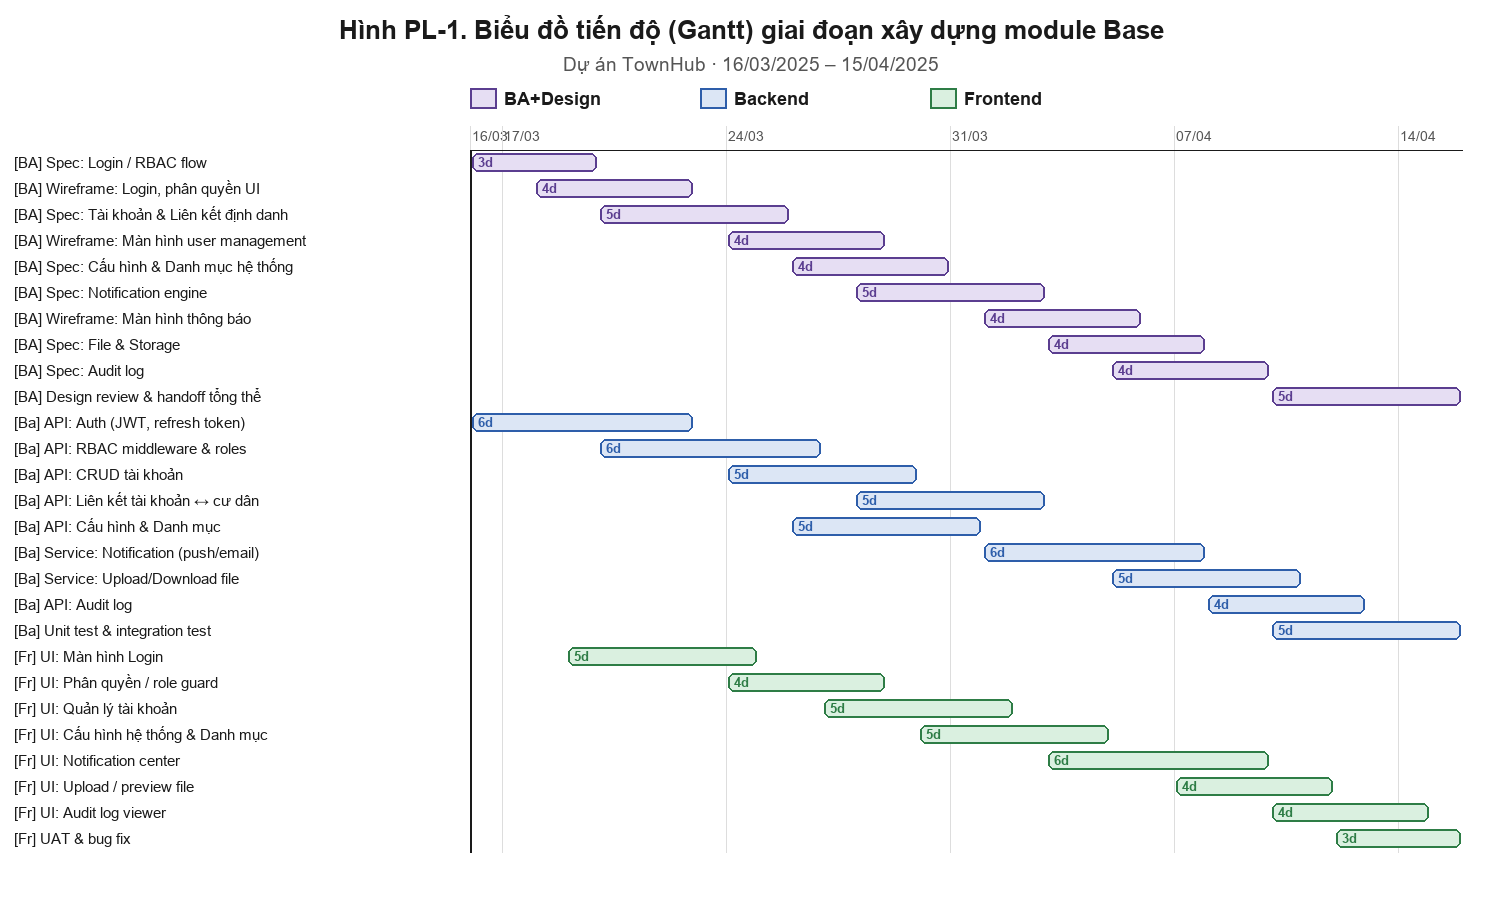
\includegraphics[width=\linewidth,height=0.82\textheight,keepaspectratio]{images/img01.png}
\caption*{\small Hình 0.1. Kế hoạch – tiến độ nhóm (biểu đồ Gantt)}
\addcontentsline{lof}{figure}{Hình 0.1. Kế hoạch – tiến độ nhóm (biểu đồ Gantt)}
\end{figure}
\begin{figure}[H]\centering
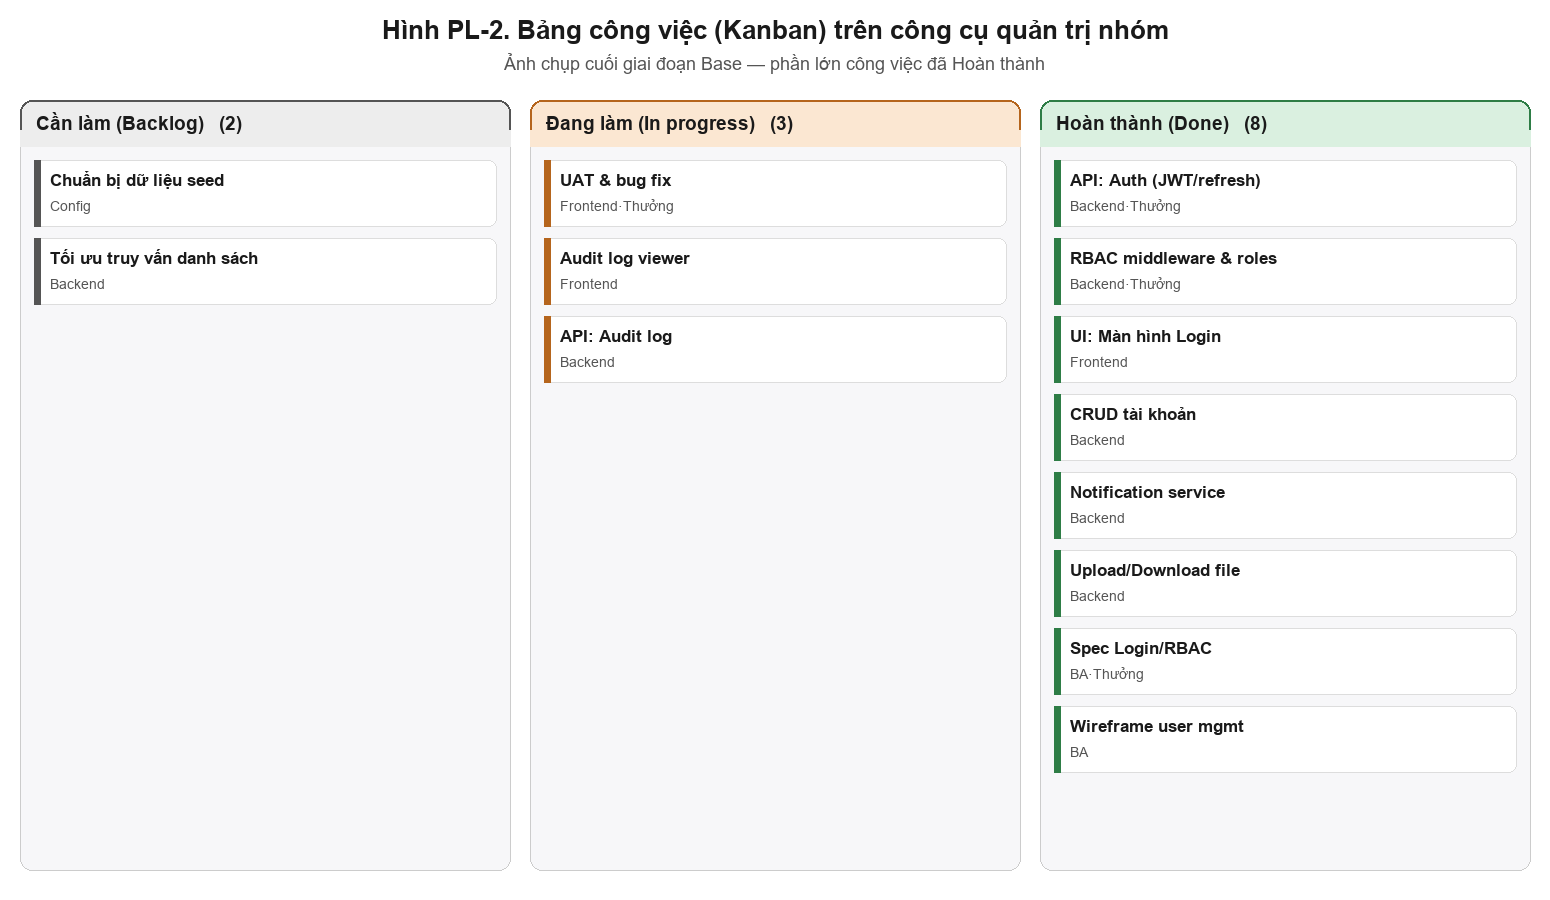
\includegraphics[width=\linewidth,height=0.82\textheight,keepaspectratio]{images/img02.png}
\caption*{\small Hình 0.2. Bảng công việc Kanban của nhóm}
\addcontentsline{lof}{figure}{Hình 0.2. Bảng công việc Kanban của nhóm}
\end{figure}
\begin{figure}[H]\centering
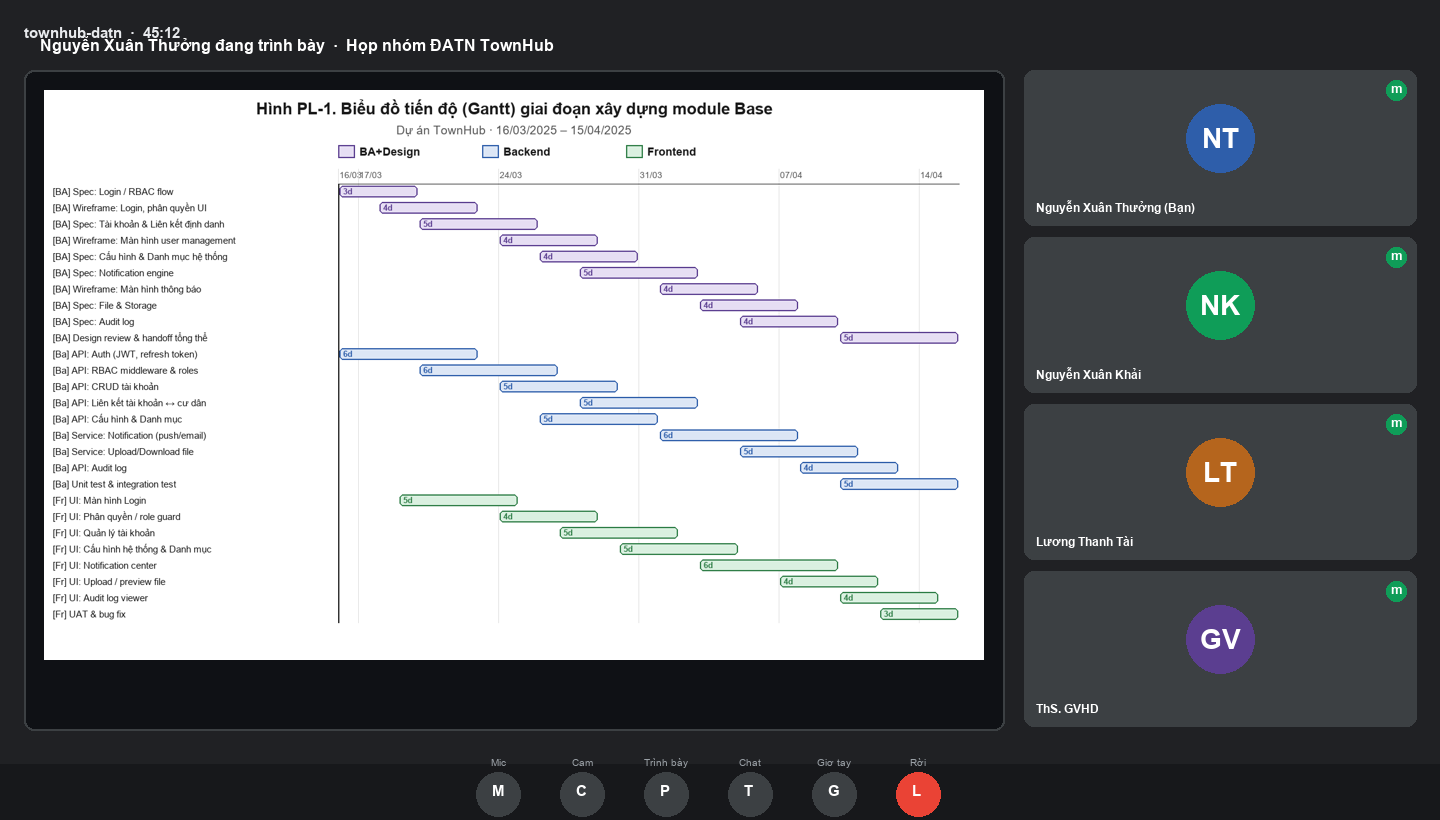
\includegraphics[width=\linewidth,height=0.82\textheight,keepaspectratio]{images/img03.png}
\caption*{\small Hình 0.3. Họp nhóm trực tuyến (đang trình bày tiến độ)}
\addcontentsline{lof}{figure}{Hình 0.3. Họp nhóm trực tuyến (đang trình bày tiến độ)}
\end{figure}
\begin{figure}[H]\centering
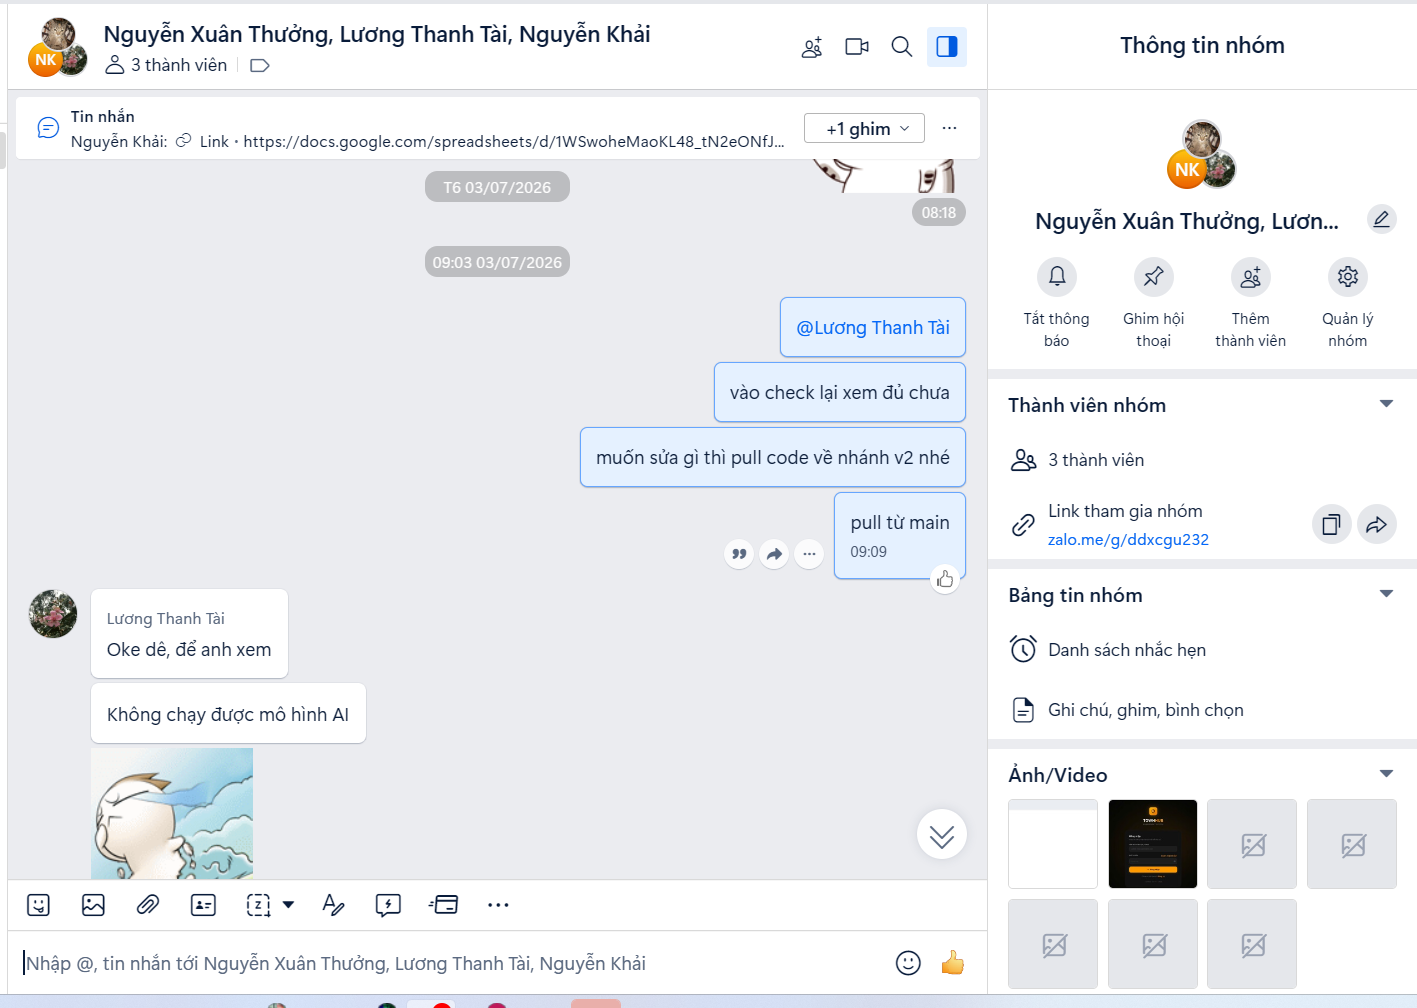
\includegraphics[width=\linewidth,height=0.82\textheight,keepaspectratio]{images/img04.png}
\caption*{\small Hình 0.4. Trao đổi công việc trên nhóm chat}
\addcontentsline{lof}{figure}{Hình 0.4. Trao đổi công việc trên nhóm chat}
\end{figure}
\begin{figure}[H]\centering
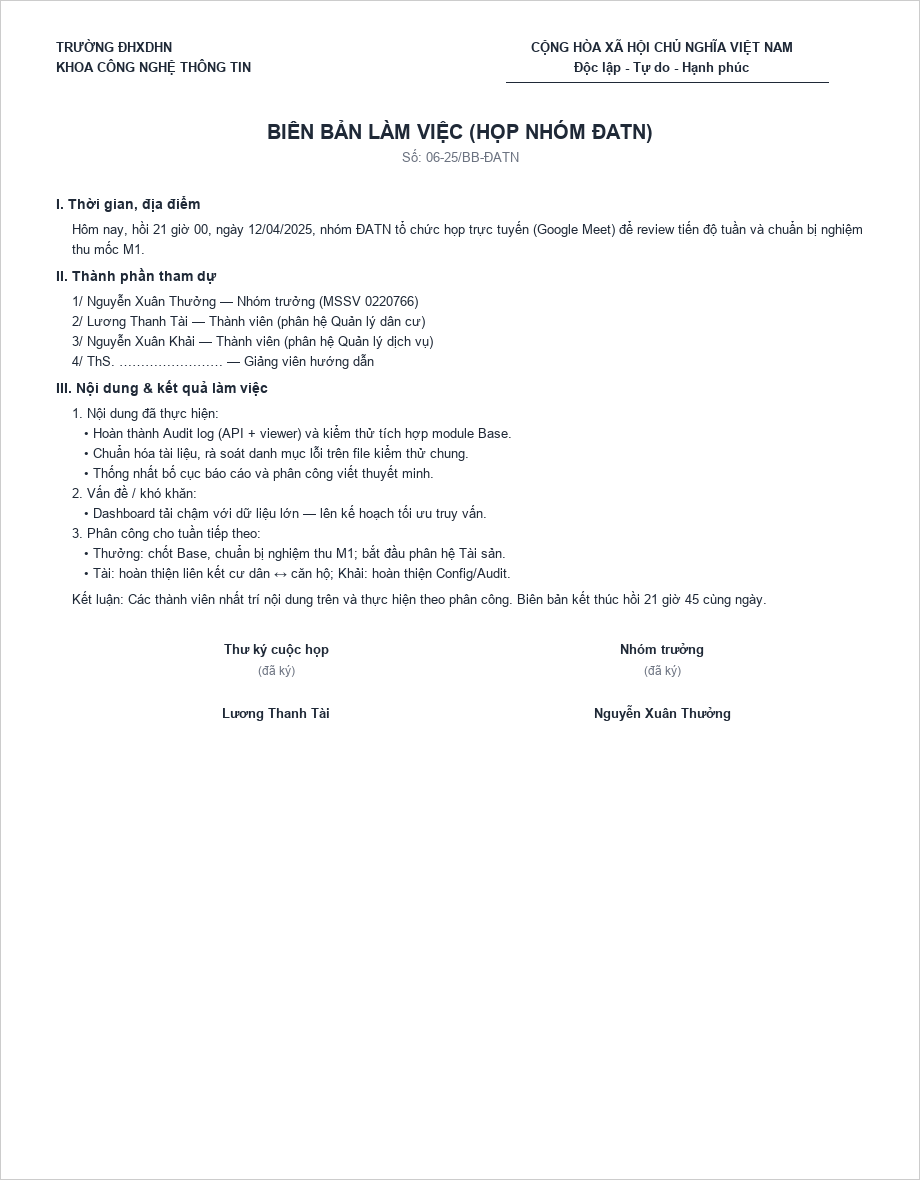
\includegraphics[width=\linewidth,height=0.82\textheight,keepaspectratio]{images/img05.png}
\caption*{\small Hình 0.5. Biên bản họp nhóm (bản mẫu)}
\addcontentsline{lof}{figure}{Hình 0.5. Biên bản họp nhóm (bản mẫu)}
\end{figure}
\phantomsection
\section*{6. Bố cục báo cáo}
\addcontentsline{toc}{section}{6. Bố cục báo cáo}
Báo cáo gồm năm chương: Chương 1 tổng quan và khảo sát bài toán; Chương 2 cơ sở lý thuyết và công nghệ; Chương 3 phân tích – thiết kế module chung (Base); Chương 4 phân hệ Quản lý tài sản do tác giả đảm nhiệm (gồm Tài sản \& bảo trì, Kho – Mua sắm – Nhà cung cấp, Sự cố \& SLA); Chương 5 triển khai, kiểm thử và đánh giá; cuối cùng là Kết luận, Tài liệu tham khảo và Phụ lục.

\phantomsection
\chapter*{Chương 1. Tổng quan và khảo sát bài toán}
\addcontentsline{toc}{chapter}{Chương 1. Tổng quan và khảo sát bài toán}
\markboth{Chương 1. Tổng quan và khảo sát bài toán}{Chương 1. Tổng quan và khảo sát bài toán}
Chương này khảo sát bài toán quản lý vận hành tòa nhà một cách có hệ thống: tổng quan nghiệp vụ và các bên liên quan, hiện trạng và vấn đề đặt ra, so sánh các giải pháp hiện có, từ đó đề xuất giải pháp cùng kiến trúc và xác định mục tiêu, phạm vi, yêu cầu của hệ thống.

\phantomsection
\section*{1.1. Tổng quan về quản lý vận hành tòa nhà}
\addcontentsline{toc}{section}{1.1. Tổng quan về quản lý vận hành tòa nhà}
Quản lý vận hành tòa nhà (building operations) là tập hợp các hoạt động nhằm duy trì tòa nhà hoạt động an toàn, hiệu quả và tiết kiệm chi phí trong suốt vòng đời. Các hoạt động này trải rộng trên ba nhóm nghiệp vụ gắn kết chặt chẽ: quản lý tài sản (thiết bị, bảo trì, vật tư – kho, mua sắm, nhà cung cấp); quản lý dân cư (hồ sơ cư dân, căn hộ, kiểm soát ra vào, thông báo); và quản lý dịch vụ (kết nối cư dân với nhà cung cấp dịch vụ, tiếp nhận và điều phối yêu cầu dịch vụ). Ba nhóm nghiệp vụ này dùng chung dữ liệu nền (người dùng, căn hộ, tòa nhà) nên rất phù hợp để số hóa trên một nền tảng tập trung.

\phantomsection
\subsection*{1.1.1. Các bên liên quan và vai trò}
\addcontentsline{toc}{subsection}{1.1.1. Các bên liên quan và vai trò}
Hệ thống phục vụ nhiều nhóm người dùng với vai trò khác nhau, trải đều trên cả ba phân hệ:

\begin{itemize}[leftmargin=1.4em,itemsep=1pt,topsep=2pt]
  \item \textbf{Chung – nền tảng: }quản trị viên (cấu hình, phân quyền); ban quản lý/quản lý vận hành (giám sát, ra quyết định, phê duyệt).
  \item \textbf{Phân hệ tài sản: }kế toán (tài sản, khấu hao, chi phí); kỹ thuật viên (bảo trì, xử lý sự cố thiết bị); thủ kho (quản lý vật tư); nhân viên mua sắm (đề xuất mua, đơn hàng).
  \item \textbf{Phân hệ dân cư: }nhân viên quản lý cư dân (lập hồ sơ cư dân, căn hộ, đăng ký nhận diện khuôn mặt ra vào); bảo vệ (giám sát ra vào).
  \item \textbf{Phân hệ dịch vụ: }cư dân (gửi yêu cầu dịch vụ, nhận thông báo); nhà cung cấp dịch vụ (đăng ký hồ sơ, niêm yết dịch vụ, tiếp nhận và xử lý yêu cầu); cư dân là chủ hộ kinh doanh (đăng ký trở thành nhà cung cấp trong tòa nhà).
\end{itemize}
Việc phân định vai trò trải đều trên cả ba phân hệ là cơ sở để thiết kế phân quyền theo vai trò (RBAC) ở phần Base.

\phantomsection
\subsection*{1.1.2. Các nghiệp vụ chính}
\addcontentsline{toc}{subsection}{1.1.2. Các nghiệp vụ chính}
Các nghiệp vụ chính được chia đều theo ba phân hệ:

\begin{itemize}[leftmargin=1.4em,itemsep=1pt,topsep=2pt]
  \item \textbf{Tài sản: }quản lý vòng đời tài sản (ghi tăng, điều chuyển, khấu hao, thanh lý); bảo trì phòng ngừa và khắc phục (lịch bảo trì, lệnh công việc); quản lý kho vật tư (nhập/xuất/kiểm kê); mua sắm (đề xuất mua, đơn mua, hóa đơn) và quản lý nhà cung cấp vật tư.
  \item \textbf{Dân cư: }quản lý hồ sơ cư dân và căn hộ/đơn vị trong tòa nhà (chủ hộ, thành viên, ngày chuyển đến); kiểm soát ra vào bằng nhận diện khuôn mặt (đăng ký khuôn mặt, ghi nhận sự kiện ra vào); gửi thông báo tới cư dân.
  \item \textbf{Dịch vụ: }đăng ký và phê duyệt hồ sơ nhà cung cấp dịch vụ; niêm yết danh mục dịch vụ (điện, nước, vệ sinh, sửa chữa, lắp đặt camera\ldots{}); tiếp nhận yêu cầu dịch vụ từ cư dân, phê duyệt của ban quản lý khi cần, phân công nhà cung cấp, theo dõi tiến độ và nghiệm thu.
  \item \textbf{Nền tảng dùng chung: }xác thực, phân quyền, quản lý người dùng, thông báo, cấu hình và báo cáo tổng hợp.
\end{itemize}
\phantomsection
\section*{1.2. Khảo sát hiện trạng và vấn đề đặt ra}
\addcontentsline{toc}{section}{1.2. Khảo sát hiện trạng và vấn đề đặt ra}
Qua khảo sát thực tế, nhóm nhận thấy phần lớn hoạt động quản lý vận hành hiện được thực hiện thủ công bằng giấy tờ hoặc bảng tính rời rạc, thiếu liên kết giữa các nghiệp vụ. Vấn đề trải đều trên cả ba phân hệ:

\begin{itemize}[leftmargin=1.4em,itemsep=1pt,topsep=2pt]
  \item \textbf{Về tài sản: }khó tra cứu nhanh thông tin một tài sản; không theo dõi được giá trị còn lại và khấu hao; dễ bỏ sót lịch bảo trì; tồn kho vật tư không chính xác; quy trình mua sắm và chứng từ khó kiểm soát; số liệu quản lý vật lý không khớp với sổ kế toán.
  \item \textbf{Về dân cư: }hồ sơ cư dân và căn hộ lưu rải rác, khó cập nhật khi có biến động (chuyển đến/đi, đổi chủ hộ); kiểm soát ra vào chủ yếu thủ công bằng thẻ hoặc ghi sổ, khó truy vết; thông báo tới cư dân phân tán qua nhiều kênh, không đồng nhất.
  \item \textbf{Về dịch vụ: }cư dân khó tìm được nhà cung cấp dịch vụ uy tín trong tòa nhà; yêu cầu dịch vụ trao đổi qua điện thoại/tin nhắn nên thiếu công cụ theo dõi trạng thái, thời gian xử lý và trách nhiệm; ban quản lý khó kiểm soát và đánh giá chất lượng nhà cung cấp.
\end{itemize}
Những hạn chế này đặt ra yêu cầu xây dựng một hệ thống tập trung, tự động hóa và liên thông dữ liệu cho cả ba phân hệ.

\phantomsection
\section*{1.3. Khảo sát các giải pháp hiện có}
\addcontentsline{toc}{section}{1.3. Khảo sát các giải pháp hiện có}
Nhóm đã khảo sát hai nhóm đối tượng: (i) các \textbf{phần mềm quản lý vận hành tòa nhà thương mại đang được triển khai thực tế tại Việt Nam} -- tiêu biểu là Building Care, Landsoft Control và CyHome; và (ii) hai cách làm phổ biến ở quy mô nhỏ là quản lý thủ công bằng bảng tính và các phần mềm quản lý bảo trì/tài sản (CMMS/EAM) quốc tế. Kết quả khảo sát được đối chiếu với hệ thống TownHub đề xuất theo các tiêu chí trải đều ba phân hệ tài sản, dân cư và dịch vụ. Các minh chứng (ảnh chụp màn hình thực tế) và đường dẫn nguồn được trích dẫn ngay bên dưới từng nội dung.

\phantomsection
\subsection*{1.3.1. Các phần mềm thương mại đang triển khai thực tế}
\addcontentsline{toc}{subsection}{1.3.1. Các phần mềm thương mại đang triển khai thực tế}

\textbf{a) Building Care (Công ty Cổ phần Công nghệ S-TECH).} Building Care là nền tảng quản lý vận hành tòa nhà toàn diện, tổ chức theo mô hình hai ứng dụng tách biệt: Web/App dành cho Ban quản lý và App riêng cho cư dân. Phần mềm gồm các phân hệ quản lý dự án -- tòa nhà, căn hộ -- cư dân, tài sản -- tài liệu (lên lịch bảo trì, bảo dưỡng và tự động nhắc khi đến hạn), nhân sự, quản lý công việc và quản lý công nợ -- phí dịch vụ. Điểm nổi bật về nghiệp vụ tài sản là số hóa yêu cầu bảo trì: thay vì dùng giấy tờ, cư dân tạo yêu cầu (\textit{ticket}) trực tiếp trên App, hệ thống tự phân công và đẩy tới thiết bị của nhân viên kỹ thuật, cập nhật trạng thái xử lý. Theo trang chủ, giải pháp đã được triển khai cho hơn 60 dự án với hơn 172 tòa nhà (Hình 1.1); tháng 6/2025, chung cư cao cấp FLC Twin Towers (265 Cầu Giấy, Hà Nội, khoảng 420 căn hộ) chính thức đưa Building Care vào vận hành (Hình 1.2).

\begin{figure}[H]\centering
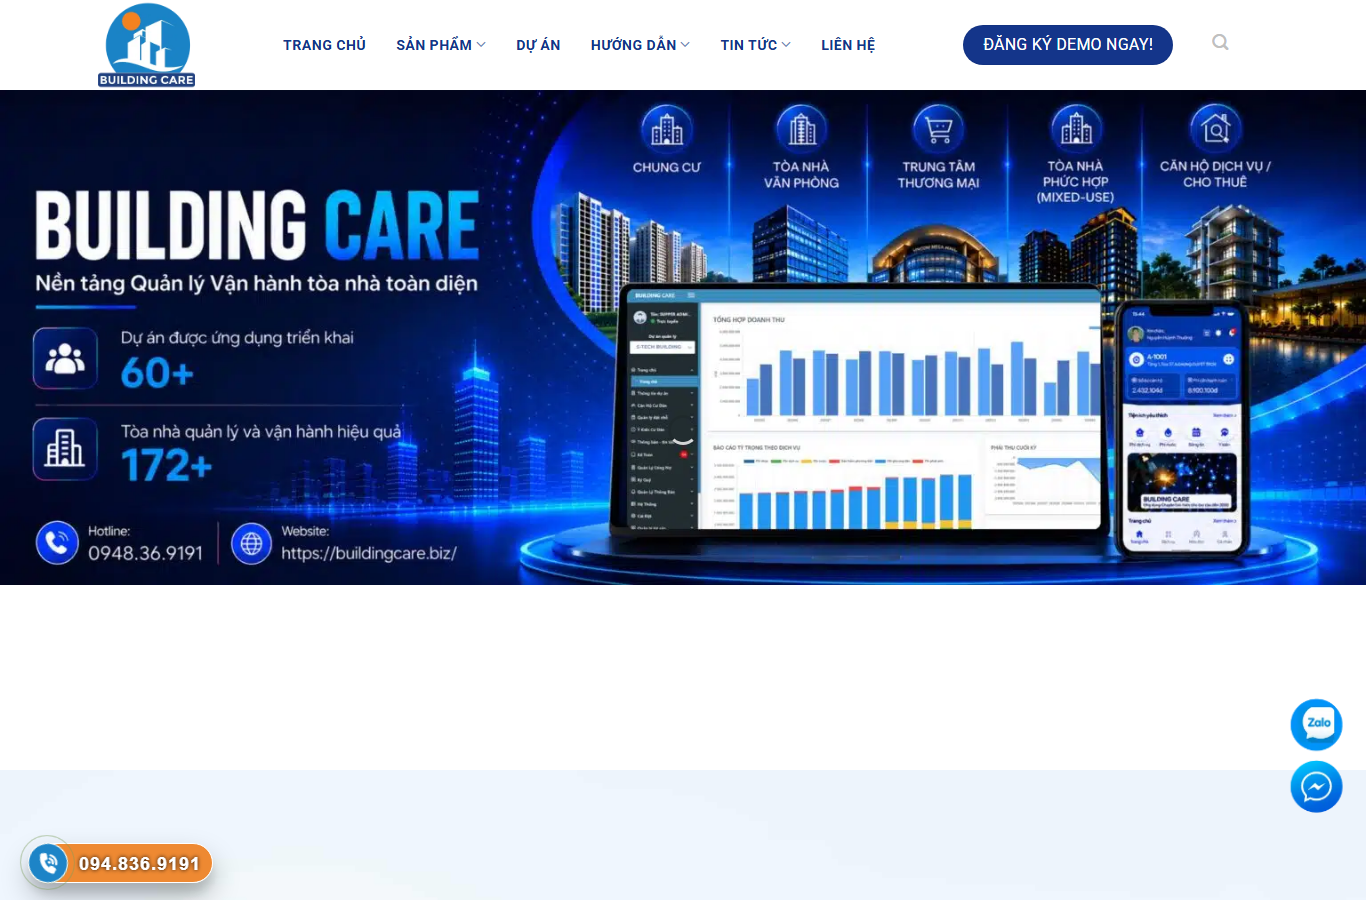
\includegraphics[width=\linewidth,height=0.42\textheight,keepaspectratio]{images/img45.png}
\caption*{\small Hình 1.1. Trang chủ nền tảng Building Care (S-TECH): mô hình Web/App BQL và App cư dân, đã triển khai 60+ dự án / 172+ tòa nhà}
\addcontentsline{lof}{figure}{Hình 1.1. Trang chủ nền tảng Building Care (S-TECH)}
\end{figure}
\noindent\textit{\small Nguồn: \url{https://buildingcare.biz/} (truy cập 07/2026).}

\begin{figure}[H]\centering
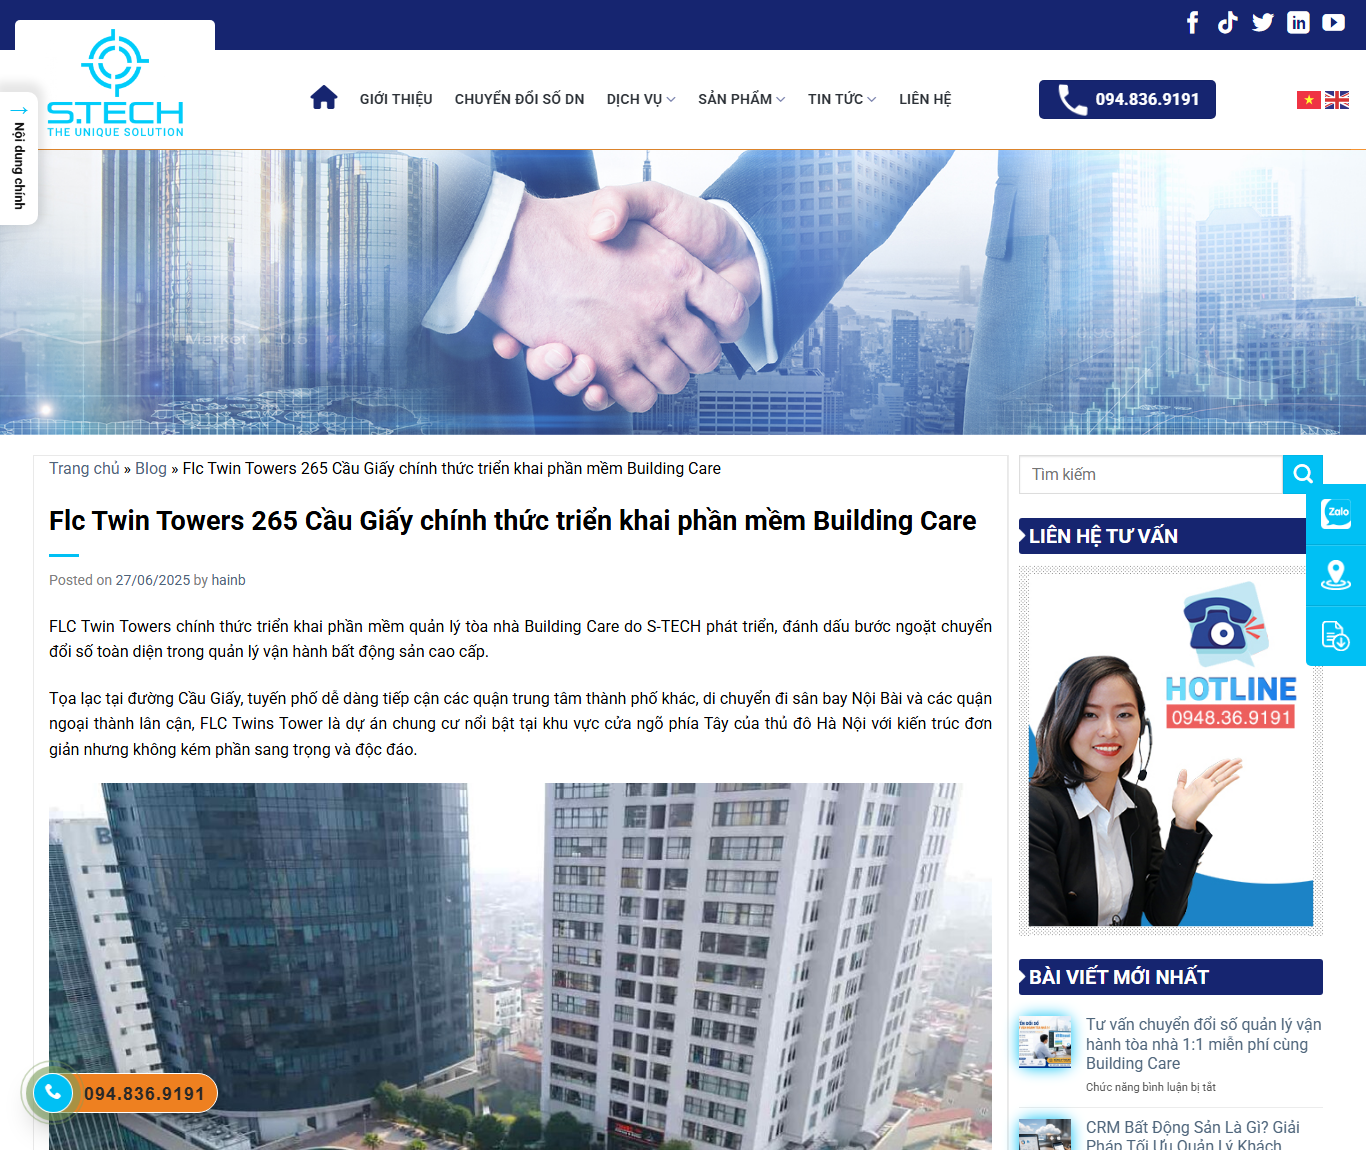
\includegraphics[width=\linewidth,height=0.5\textheight,keepaspectratio]{images/img46.png}
\caption*{\small Hình 1.2. Thông cáo triển khai Building Care tại FLC Twin Towers 265 Cầu Giấy (đăng 27/06/2025)}
\addcontentsline{lof}{figure}{Hình 1.2. Thông cáo triển khai Building Care tại FLC Twin Towers}
\end{figure}
\noindent\textit{\small Nguồn: \url{https://s-tech.info/flc-twin-towers-265-cau-giay-chinh-thuc-trien-khai-phan-mem-building-care/}}

\textbf{b) Landsoft Control (Công ty Landsoft -- phân phối qua DIP Holding).} Landsoft Control tập trung vào quản lý vòng đời thiết bị (\textit{lifecycle management}): theo dõi danh mục tài sản -- trang thiết bị kỹ thuật, lập kế hoạch bảo trì -- bảo dưỡng định kỳ, ghi nhận lịch sử sửa chữa và tiếp nhận yêu cầu sửa chữa từ cư dân qua module kỹ thuật. Đây là nền tảng mở, tích hợp hệ thống bãi đỗ xe thông minh qua API, tích hợp Zalo OA để gửi thông báo phí, và đặc biệt đồng bộ với ứng dụng cư dân ``My Home Vime'' tích hợp sẵn cổng thanh toán VNPay và Viettel Pay -- giúp thu phí dịch vụ (phí quản lý, quỹ bảo trì, điện nước) và tự động gạch nợ trên hệ thống kế toán mà không cần đối soát thủ công. Phần mềm đã đồng hành cùng Xuân Mai Corp từ năm 2016 cho 11 dự án tòa nhà lớn (Hình 1.3) và được Geleximco ứng dụng để số hóa quản lý chuỗi tòa nhà (Hình 1.4), bên cạnh các khách hàng như SunGroup, Vietracimex.

\begin{figure}[H]\centering
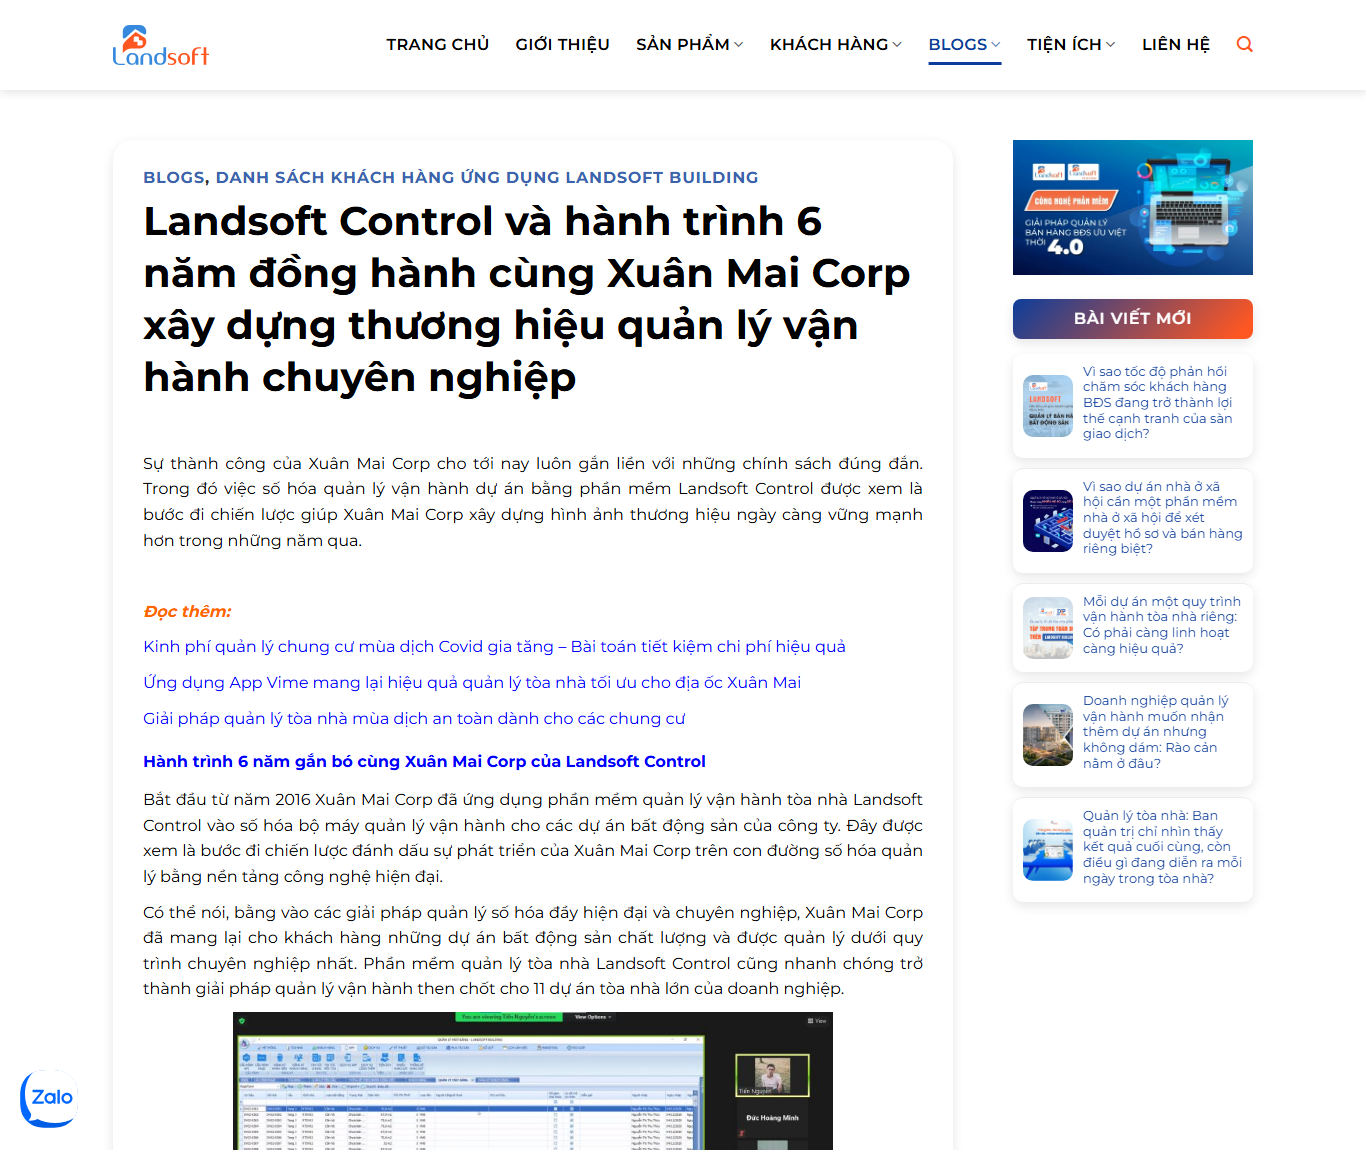
\includegraphics[width=\linewidth,height=0.5\textheight,keepaspectratio]{images/img47.png}
\caption*{\small Hình 1.3. Landsoft Control đồng hành cùng Xuân Mai Corp (từ 2016, 11 dự án tòa nhà); ảnh dưới bài là giao diện phần mềm Landsoft Building}
\addcontentsline{lof}{figure}{Hình 1.3. Landsoft Control triển khai cho Xuân Mai Corp}
\end{figure}
\noindent\textit{\small Nguồn: \url{https://landsoft.com.vn/landsoft-control-va-hanh-trinh-6-nam-dong-hanh-cung-xuan-mai-corp-xay-dung-thuong-hieu-quan-ly-van-hanh-chuyen-nghiep/}}

\begin{figure}[H]\centering
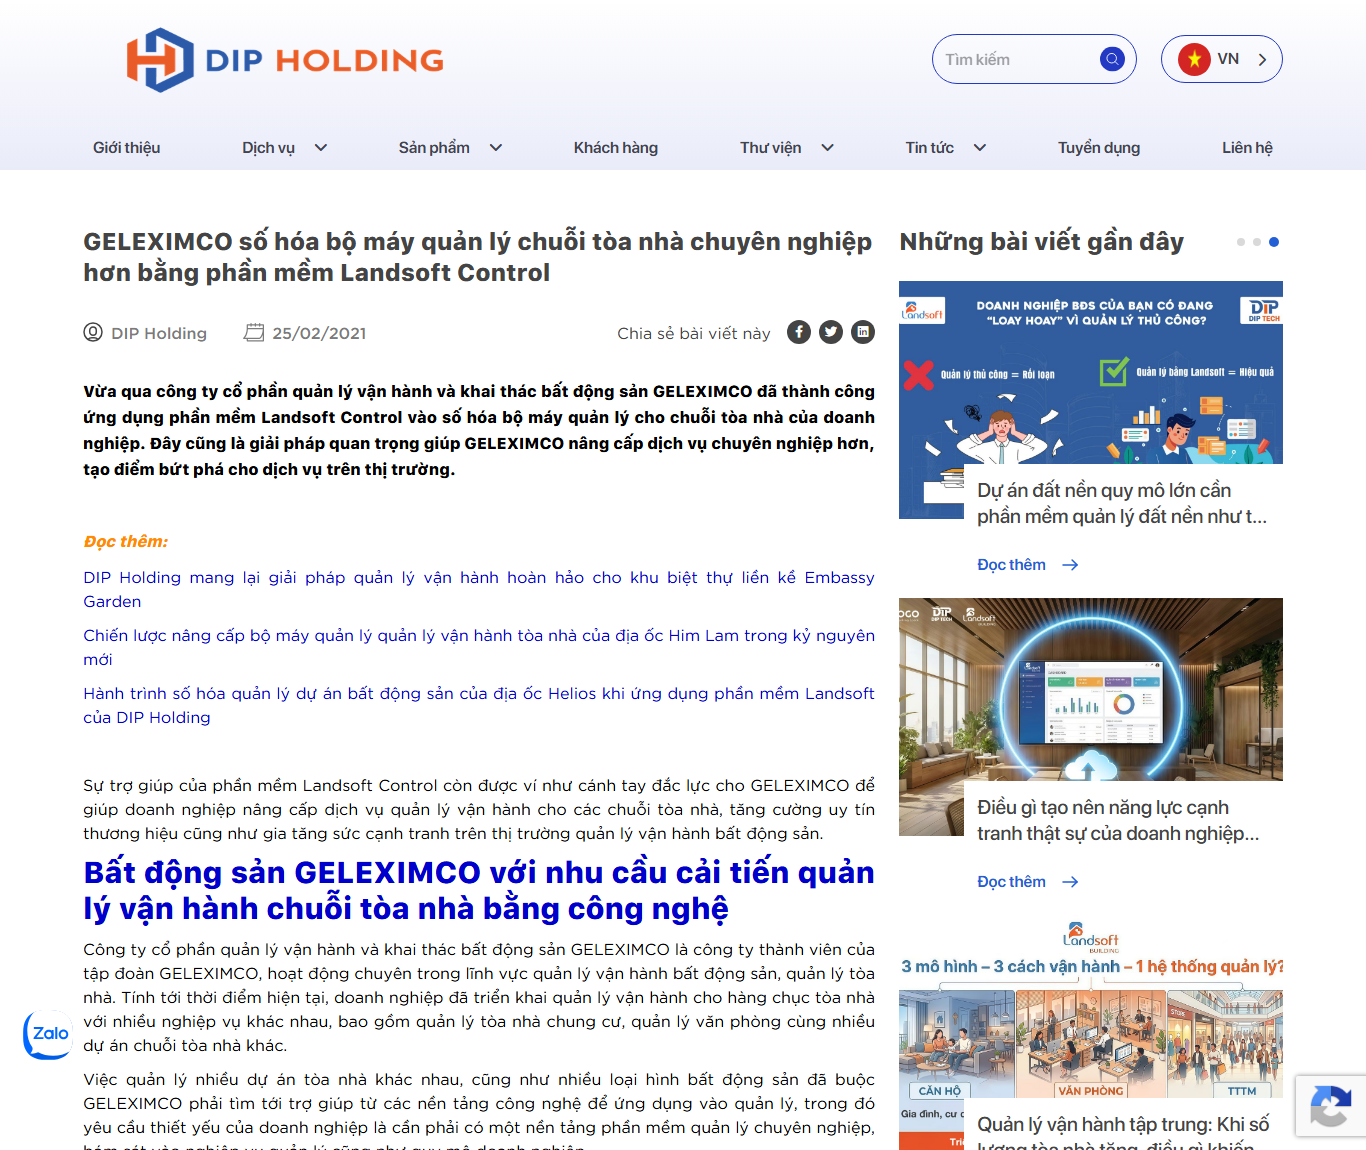
\includegraphics[width=\linewidth,height=0.5\textheight,keepaspectratio]{images/img48.png}
\caption*{\small Hình 1.4. Geleximco số hóa bộ máy quản lý chuỗi tòa nhà bằng Landsoft Control (DIP Holding, 25/02/2021)}
\addcontentsline{lof}{figure}{Hình 1.4. Geleximco ứng dụng Landsoft Control}
\end{figure}
\noindent\textit{\small Nguồn: \url{https://dip.vn/geleximco-so-hoa-bo-may-quan-ly-chuoi-toa-nha-chuyen-nghiep-hon-bang-phan-mem-landsoft-control/}}

\textbf{c) CyHome (Công ty CYFEER JSC).} CyHome là nền tảng quản trị chung cư cung cấp theo mô hình SaaS (\textit{Software as a Service}) trên hạ tầng đám mây Amazon Web Services, thu phí theo đầu căn hộ (tham khảo khoảng 10.000đ/căn/tháng -- một tòa 300 căn trả phí phần mềm khoảng 3 triệu đồng/tháng). Hệ sinh thái gồm App cư dân, Web/App Ban quản lý và đặc biệt App chuyên biệt cho kỹ thuật viên \textbf{CyHome PMS}: kỹ thuật viên đi chốt số dịch vụ định kỳ (đồng hồ điện, nước), nhập số liệu và chụp ảnh lưu chứng cứ trực tiếp tại hiện trường lên đám mây, qua đó khóa chặt lỗ hổng gian lận và sai sót dữ liệu (Hình 1.6). CyHome đã được hơn 200 dự án sử dụng, phục vụ hơn 180.000 cư dân, với các đơn vị quản lý vận hành như CBRE, Visaho, Proman và chủ đầu tư như Vingroup, Novaland; nền tảng đạt giải Sao Khuê 2022 (Hình 1.5).

\begin{figure}[H]\centering
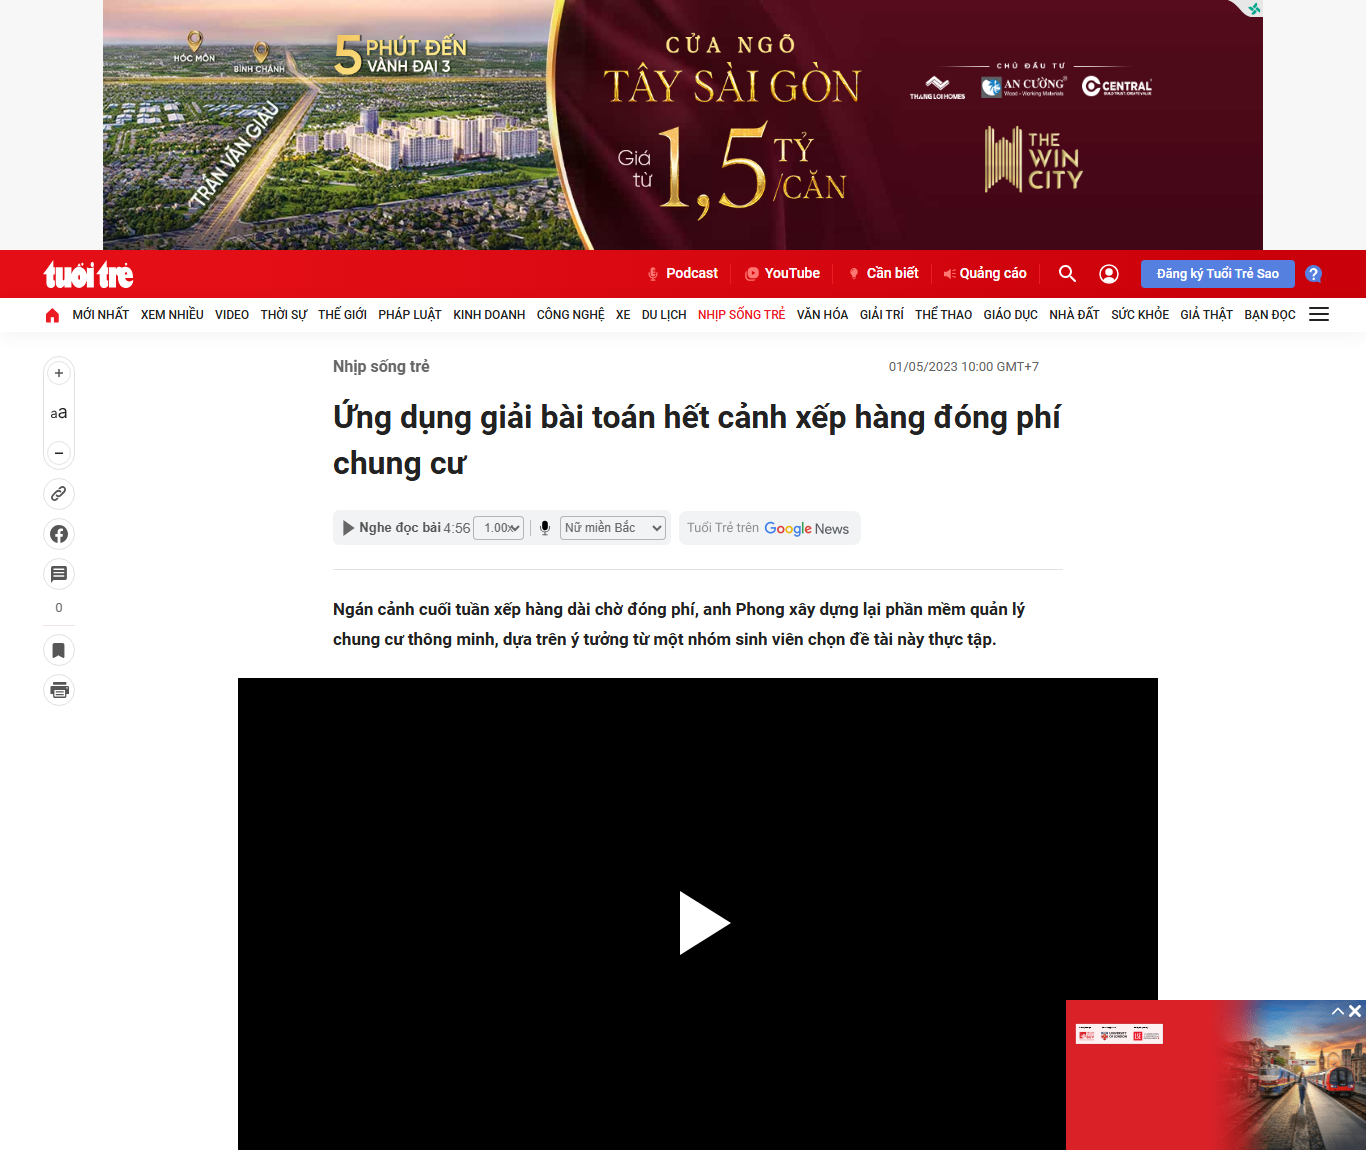
\includegraphics[width=\linewidth,height=0.5\textheight,keepaspectratio]{images/img50.png}
\caption*{\small Hình 1.5. Báo Tuổi Trẻ phân tích mô hình thu phí theo căn hộ của CyHome (01/05/2023)}
\addcontentsline{lof}{figure}{Hình 1.5. Bài báo Tuổi Trẻ về mô hình phí của CyHome}
\end{figure}
\noindent\textit{\small Nguồn: \url{https://tuoitre.vn/ung-dung-giai-bai-toan-het-canh-xep-hang-dong-phi-chung-cu-20230425232909509.htm}}

\begin{figure}[H]\centering
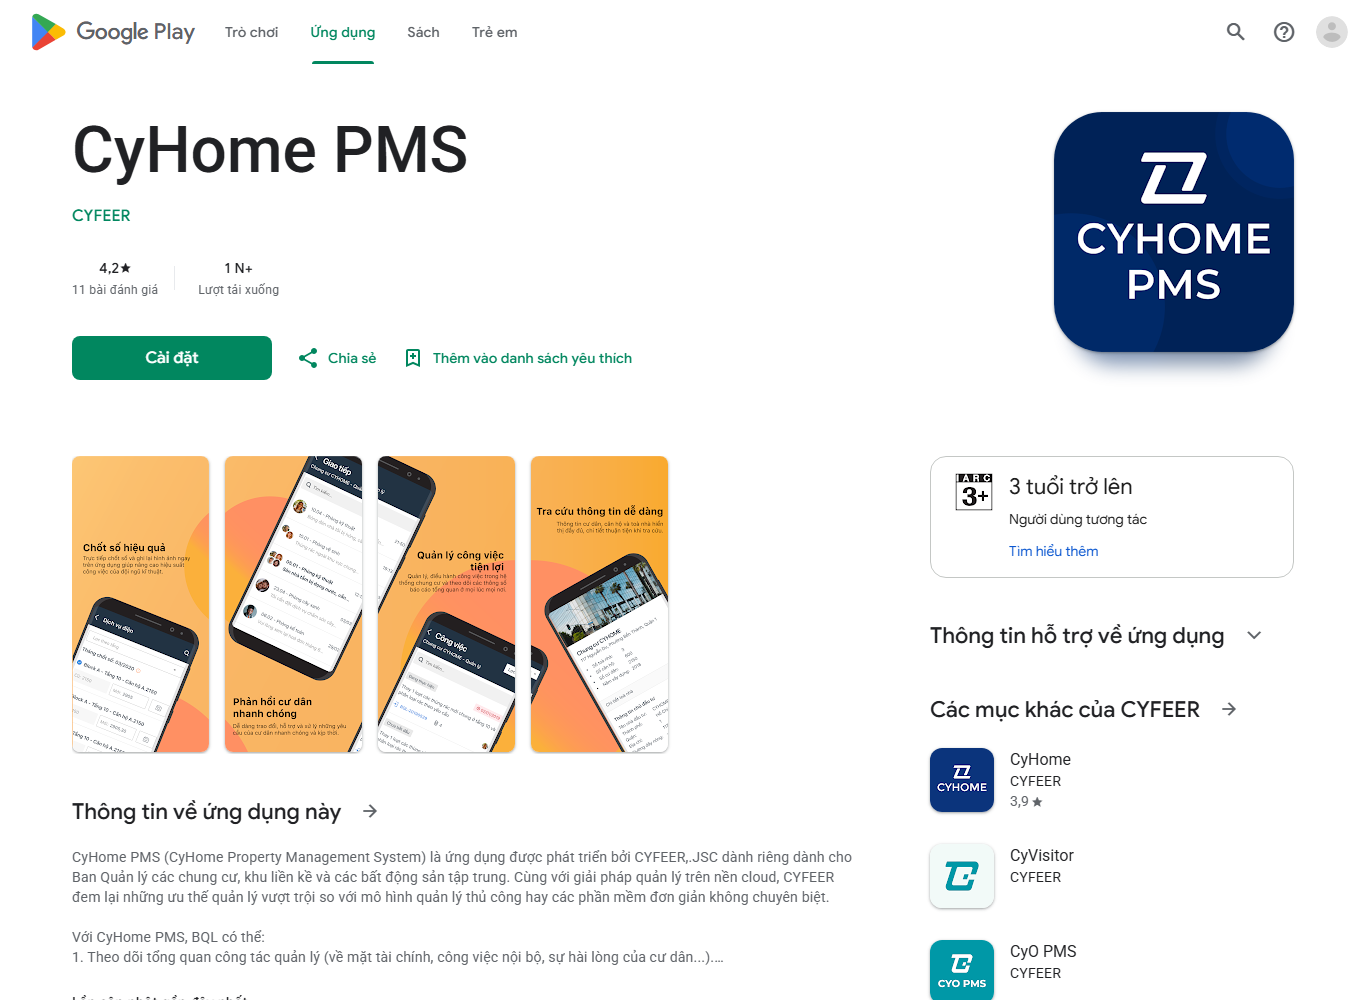
\includegraphics[width=\linewidth,height=0.5\textheight,keepaspectratio]{images/img51.png}
\caption*{\small Hình 1.6. Ứng dụng CyHome PMS dành cho kỹ thuật viên trên Google Play (CYFEER, 4,2\textasteriskcentered): chốt số, phản hồi cư dân, quản lý công việc tại hiện trường}
\addcontentsline{lof}{figure}{Hình 1.6. Ứng dụng CyHome PMS cho kỹ thuật viên (Google Play)}
\end{figure}
\noindent\textit{\small Nguồn: \url{https://play.google.com/store/apps/details?id=com.cyfeer.cyhome_manager&hl=vi}}

\phantomsection
\subsection*{1.3.2. So sánh tổng hợp và định vị TownHub}
\addcontentsline{toc}{subsection}{1.3.2. So sánh tổng hợp và định vị TownHub}
Bảng dưới đây so sánh ba nhóm giải pháp -- quản lý thủ công (Excel), phần mềm thương mại (đại diện là Building Care, Landsoft Control, CyHome) và TownHub đề xuất -- theo các tiêu chí trải đều ba phân hệ tài sản, dân cư và dịch vụ:

\begin{center}{\singlespacing\renewcommand{\arraystretch}{1.25}
\begin{tabular}{|>{\raggedright\arraybackslash}p{\dimexpr\linewidth/4-2\tabcolsep-\arrayrulewidth\relax}|>{\raggedright\arraybackslash}p{\dimexpr\linewidth/4-2\tabcolsep-\arrayrulewidth\relax}|>{\raggedright\arraybackslash}p{\dimexpr\linewidth/4-2\tabcolsep-\arrayrulewidth\relax}|>{\raggedright\arraybackslash}p{\dimexpr\linewidth/4-2\tabcolsep-\arrayrulewidth\relax}|}
\hline
Tiêu chí & Quản lý thủ công (Excel) & PM thương mại (Building Care / Landsoft / CyHome) & TownHub (đề xuất) \\ \hline
\textbf{Tài sản – }Vòng đời \& khấu hao & Thủ công, dễ sai & Có & Có, tự động \\ \hline
\textbf{Tài sản – }Bảo trì phòng ngừa (PM/​WO) & Không & Có & Có \\ \hline
\textbf{Tài sản – }Kho vật tư \& mua sắm (PR/​PO) & Rời rạc & Một phần & Có, liên thông \\ \hline
\textbf{Tài sản – }OCR hóa đơn tiếng Việt & Không & Hiếm/Không & Có (VietOCR/PaddleOCR) \\ \hline
\textbf{Tài sản – }Tích hợp kế toán \& chi phí & Thủ công & Tùy sản phẩm & Có (bút toán Nợ/Có) \\ \hline
\textbf{Dân cư – }Hồ sơ cư dân \& căn hộ & Rời rạc & Có & Có, tập trung \\ \hline
\textbf{Dân cư – }Kiểm soát ra vào & Thủ công (thẻ/sổ) & Tùy tích hợp & Có (nhận diện khuôn mặt) \\ \hline
\textbf{Dịch vụ – }Kết nối cư dân – NCC dịch vụ & Không & Một phần & Có (niêm yết dịch vụ) \\ \hline
\textbf{Dịch vụ – }Yêu cầu \& phê duyệt, theo dõi & Không & Có & Có, có quy trình duyệt \\ \hline
\textbf{Dịch vụ – }Thanh toán phí \& gạch nợ tự động & Không & \textbf{Có} (VNPay/Viettel Pay) & Định hướng bổ sung \\ \hline
\textbf{Nền tảng – }Ứng dụng di động cư dân/KTV & Không & \textbf{Có} (App gốc) & Web responsive \\ \hline
\textbf{Nền tảng – }Chi phí \& khả năng tùy biến & Thấp/Rời rạc & Cao, đóng, khó tùy biến & Thấp, tự chủ mã nguồn \\ \hline
\textbf{Nền tảng – }Quy mô đã triển khai thực tế & -- & \textbf{Lớn} (60–200+ dự án) & Đồ án/nguyên mẫu \\ \hline
\end{tabular}}\end{center}
\textbf{Nhận xét.} Ba phần mềm thương mại đều đã trưởng thành và triển khai ở quy mô lớn, mạnh về quản lý tài sản -- bảo trì, tương tác cư dân qua App di động và (với Landsoft, CyHome) thu phí -- thanh toán trực tuyến. Tuy nhiên chúng chủ yếu là sản phẩm đóng, chi phí bản quyền/thuê bao cao và khó tùy biến theo đặc thù từng đơn vị; phần lớn tập trung vào tài sản -- phí dịch vụ mà ít hoặc chưa có: (a) bóc tách hóa đơn mua sắm bằng OCR tiếng Việt; (b) tích hợp kế toán tài sản với bút toán Nợ/Có (ghi tăng, khấu hao, thanh lý); (c) kiểm soát ra vào bằng nhận diện khuôn mặt. Đây chính là những điểm khác biệt mà TownHub hướng tới. Ở chiều ngược lại, các sản phẩm thương mại đang vượt trội hơn TownHub ở: tích hợp cổng thanh toán và tự động gạch nợ (Landsoft), ứng dụng di động gốc cho cư dân/kỹ thuật viên (CyHome, Building Care) và mức độ triển khai thực tế ở hàng trăm dự án -- đây là những hướng hoàn thiện TownHub có thể kế thừa trong tương lai. Quản lý thủ công (Excel) tuy rẻ nhưng rời rạc và dễ sai sót trên cả ba phân hệ. Tựu trung, TownHub định vị là nền tảng \textit{module hóa, tự chủ mã nguồn, chi phí thấp}, tích hợp sẵn OCR -- kế toán -- nhận diện khuôn mặt và liên thông cả ba phân hệ tài sản, dân cư, dịch vụ; đó là khoảng trống mà các giải pháp hiện có chưa lấp đầy trọn vẹn.

\phantomsection
\section*{1.4. Đề xuất giải pháp và kiến trúc module hoá}
\addcontentsline{toc}{section}{1.4. Đề xuất giải pháp và kiến trúc module hoá}
Trên cơ sở khảo sát, nhóm chúng em đề xuất xây dựng hệ thống TownHub theo kiến trúc module hóa – phân chia module độc lập nhưng liên thông. Về mặt nghiệp vụ, hệ thống gồm ba phân hệ ngang hàng – Tài sản, Dân cư và Dịch vụ – cùng kế thừa lớp nền tảng Base (lõi dùng chung: xác thực – phân quyền, người dùng, thông báo, cấu hình, báo cáo, cùng dữ liệu nền dân cư và dịch vụ). Về triển khai, backend được chia thành ba module Auth, Base và Asset tương ứng ba schema cơ sở dữ liệu auth, base và asset (nghiệp vụ dân cư và dịch vụ nằm trong Base); các module giao tiếp qua định danh cross-service dạng Guid, không phụ thuộc chặt vào nhau.

Cách tiếp cận này giúp: tránh trùng lặp chức năng nền tảng; cho phép các thành viên phát triển song song phân hệ riêng của mình (tài sản, dân cư, dịch vụ) mà vẫn kế thừa dữ liệu và dịch vụ dùng chung; dễ bảo trì, kiểm thử và triển khai từng phần; đồng thời thuận lợi cho việc mở rộng thêm phân hệ mới trong tương lai. Đây cũng là cách nhóm phân định rõ khối lượng công việc: phần chung do cả nhóm chịu trách nhiệm, mỗi phân hệ nghiệp vụ thể hiện đóng góp cá nhân của từng thành viên.

\phantomsection
\section*{1.5. Mục tiêu, phạm vi và yêu cầu hệ thống}
\addcontentsline{toc}{section}{1.5. Mục tiêu, phạm vi và yêu cầu hệ thống}
\phantomsection
\subsection*{1.5.1. Yêu cầu chức năng}
\addcontentsline{toc}{subsection}{1.5.1. Yêu cầu chức năng}
\begin{itemize}[leftmargin=1.4em,itemsep=1pt,topsep=2pt]
  \item \textbf{Xác thực \& phân quyền (chung): }đăng nhập đa phương thức, MFA, phân quyền theo vai trò (RBAC); quản lý người dùng, thông báo, cấu hình, danh mục dùng chung và báo cáo tổng hợp.
  \item \textbf{Phân hệ Tài sản: }danh mục, ghi tăng, mã QR, điều chuyển, khấu hao, thanh lý; lịch bảo trì định kỳ, lệnh công việc, checklist, nghiệm thu; tồn kho, PR/PO/hóa đơn, hợp đồng, đánh giá NCC, OCR hóa đơn.
  \item \textbf{Phân hệ Dân cư: }quản lý hồ sơ cư dân, căn hộ/đơn vị và tòa nhà; đăng ký nhận diện khuôn mặt và ghi nhận sự kiện kiểm soát ra vào; gửi và theo dõi thông báo tới cư dân.
  \item \textbf{Phân hệ Dịch vụ: }đăng ký và phê duyệt nhà cung cấp dịch vụ; niêm yết danh mục dịch vụ; cư dân gửi yêu cầu dịch vụ; quy trình phê duyệt của ban quản lý, phân công nhà cung cấp, theo dõi trạng thái và nghiệm thu.
\end{itemize}
\phantomsection
\subsection*{1.5.2. Yêu cầu phi chức năng}
\addcontentsline{toc}{subsection}{1.5.2. Yêu cầu phi chức năng}
\begin{itemize}[leftmargin=1.4em,itemsep=1pt,topsep=2pt]
  \item \textbf{Bảo mật: }xác thực JWT, phân quyền tối thiểu theo vai trò, bảo vệ dữ liệu nhạy cảm (thông tin cư dân, dữ liệu sinh trắc học khuôn mặt).
  \item \textbf{Hiệu năng: }phản hồi nhanh, hỗ trợ phân trang – lọc trên các danh sách lớn (tài sản, cư dân, yêu cầu dịch vụ).
  \item Khả năng mở rộng và bảo trì: kiến trúc module, tách schema, chuẩn hóa API.
  \item Tính khả dụng và trải nghiệm: giao diện thân thiện, responsive, hỗ trợ đa thiết bị.
\end{itemize}
\phantomsection
\section*{1.6. Kết luận chương}
\addcontentsline{toc}{section}{1.6. Kết luận chương}
Chương 1 đã khảo sát nghiệp vụ, phân tích hiện trạng và các giải pháp hiện có trên cả ba phân hệ – tài sản, dân cư và dịch vụ – từ đó đề xuất giải pháp TownHub theo kiến trúc module hóa cùng mục tiêu, phạm vi và yêu cầu cụ thể. Đây là căn cứ để lựa chọn công nghệ ở Chương 2 và thiết kế hệ thống ở các chương tiếp theo.

\phantomsection
\chapter*{Chương 2. Cơ sở lý thuyết và công nghệ sử dụng}
\addcontentsline{toc}{chapter}{Chương 2. Cơ sở lý thuyết và công nghệ sử dụng}
\markboth{Chương 2. Cơ sở lý thuyết và công nghệ sử dụng}{Chương 2. Cơ sở lý thuyết và công nghệ sử dụng}
Chương này trình bày kiến trúc phần mềm áp dụng và các công nghệ được lựa chọn để xây dựng hệ thống TownHub, bao gồm nền tảng backend, frontend, cơ sở dữ liệu, cơ chế bảo mật – phân quyền, hạ tầng phụ trợ, thành phần AI/OCR và công cụ triển khai. Các lựa chọn công nghệ được cả nhóm thảo luận và thống nhất ngay từ giai đoạn thiết kế để bảo đảm các module tích hợp đồng nhất, đồng thời bám sát yêu cầu đã nêu ở Chương 1 và hiện trạng mã nguồn thực tế của dự án.

\phantomsection
\section*{2.1. Kiến trúc phần mềm áp dụng}
\addcontentsline{toc}{section}{2.1. Kiến trúc phần mềm áp dụng}
Hệ thống áp dụng mô hình client–server, giao tiếp qua REST API định dạng JSON và xác thực bằng JWT. Tầng backend tổ chức theo kiến trúc phân tầng (layered architecture): Controllers tiếp nhận yêu cầu và kiểm tra quyền $\rightarrow$ ApplicationService xử lý logic nghiệp vụ $\rightarrow$ Domain chứa thực thể và Infrastructure đảm nhiệm truy cập dữ liệu qua EF Core. Toàn bộ backend được chia thành ba module độc lập Auth, Base và Asset, mỗi module có đầy đủ bốn tầng và tương ứng một schema cơ sở dữ liệu, giúp phân tách trách nhiệm rõ ràng và cho phép phát triển song song.

\phantomsection
\section*{2.2. Công nghệ Backend (.NET 8 Web API)}
\addcontentsline{toc}{section}{2.2. Công nghệ Backend (.NET 8 Web API)}
Backend được xây dựng bằng .NET 8 với Entity Framework Core làm ORM truy cập PostgreSQL. Các thành phần chính được tổng hợp trong Bảng 2.1.

\begin{center}{\singlespacing\renewcommand{\arraystretch}{1.25}
\begin{tabular}{|>{\raggedright\arraybackslash}p{\dimexpr\linewidth/2-2\tabcolsep-\arrayrulewidth\relax}|>{\raggedright\arraybackslash}p{\dimexpr\linewidth/2-2\tabcolsep-\arrayrulewidth\relax}|}
\hline
\textbf{Hạng mục} & \textbf{Công nghệ} \\ \hline
Framework & .NET 8.​0 (nullable + implicit usings) \\ \hline
ORM & Entity Framework Core 8.​0.​11 \\ \hline
CSDL & PostgreSQL (Npgsql.​EntityFrameworkCore.​PostgreSQL) \\ \hline
API Docs & Swashbuckle / Swagger 6.​6.​2 \\ \hline
Xác thực & JWT Bearer, Google OAuth 2.​0, Identity.​Core \\ \hline
MFA & Otp.​NET (TOTP) \\ \hline
Cache / Session & StackExchange.​Redis \\ \hline
Email & MailKit \\ \hline
Lưu trữ file & CloudinaryDotNet \\ \hline
\end{tabular}}\end{center}
\phantomsection
\section*{2.3. Công nghệ Frontend (Next.js 16 + React 19)}
\addcontentsline{toc}{section}{2.3. Công nghệ Frontend (Next.js 16 + React 19)}
Giao diện được phát triển bằng Next.js 16 (App Router) và React 19 với TypeScript, sử dụng Tailwind CSS và bộ component Radix UI để bảo đảm tính nhất quán và khả năng tùy biến. Các thư viện hỗ trợ được liệt kê trong Bảng 2.2.

\begin{center}{\singlespacing\renewcommand{\arraystretch}{1.25}
\begin{tabular}{|>{\raggedright\arraybackslash}p{\dimexpr\linewidth/2-2\tabcolsep-\arrayrulewidth\relax}|>{\raggedright\arraybackslash}p{\dimexpr\linewidth/2-2\tabcolsep-\arrayrulewidth\relax}|}
\hline
\textbf{Hạng mục} & \textbf{Công nghệ} \\ \hline
Framework & Next.​js 16.​2.​1 (App Router) \\ \hline
UI & React 19, TypeScript 5 (strict) \\ \hline
Styling & Tailwind CSS v4 (CSS variables, dark mode) \\ \hline
Component & Radix UI (29+ primitives) \\ \hline
Form / MFA & react-hook-form, input-otp \\ \hline
Biểu đồ & recharts \\ \hline
QR Code & qrcode (sinh), jsqr (quét) \\ \hline
\end{tabular}}\end{center}
Toàn bộ lời gọi API được tập trung ở tầng client (lib/api.ts) và tự động gắn token xác thực; trạng thái người dùng, quyền và phiên được quản lý qua AuthContext. Menu và chức năng hiển thị theo quyền (RBAC phía frontend) đồng bộ với backend.

\phantomsection
\section*{2.4. Cơ sở dữ liệu PostgreSQL}
\addcontentsline{toc}{section}{2.4. Cơ sở dữ liệu PostgreSQL}
Hệ thống sử dụng PostgreSQL - hệ quản trị cơ sở dữ liệu quan hệ mã nguồn mở, mạnh về toàn vẹn dữ liệu, kiểu dữ liệu phong phú (JSON, ENUM) và giao dịch (transaction). Dữ liệu được tổ chức thành ba schema độc lập auth, base và asset tương ứng ba module backend, giúp cô lập dữ liệu giữa các module và thuận tiện phân quyền, sao lưu. EF Core quản lý ánh xạ thực thể và migration để đồng bộ lược đồ.

\phantomsection
\section*{2.5. Bảo mật và phân quyền (JWT, OAuth, MFA/TOTP, RBAC)}
\addcontentsline{toc}{section}{2.5. Bảo mật và phân quyền (JWT, OAuth, MFA/TOTP, RBAC)}
Về xác thực, hệ thống hỗ trợ ba phương thức: email/mật khẩu, Google OAuth 2.0 và luồng riêng cho di động. Sau khi đăng nhập, hệ thống cấp AccessToken (hiệu lực khoảng 30 phút) và RefreshToken (khoảng 7 ngày), áp dụng cơ chế token rotation và trường tokenVersion để vô hiệu hóa token khi cần. Với web, token lưu trong cookie HttpOnly kèm CSRF token; phiên được quản lý theo thiết bị, cho phép đăng xuất trên một hoặc tất cả thiết bị. Bảo mật được tăng cường bằng xác thực đa yếu tố (MFA) dùng mã OTP theo thời gian (TOTP).

Về phân quyền, hệ thống áp dụng mô hình RBAC (Role-Based Access Control): quyền định nghĩa chi tiết theo cặp resource + action, gán cho vai trò và vai trò gán cho người dùng; mỗi API được bảo vệ bằng policy tương ứng. Chi tiết thiết kế được trình bày ở Chương 3.

\phantomsection
\section*{2.6. Hạ tầng cache, lưu trữ và email}
\addcontentsline{toc}{section}{2.6. Hạ tầng cache, lưu trữ và email}
Redis được dùng làm bộ nhớ đệm và lưu trạng thái phiên/MFA, giúp giảm tải truy vấn và tăng tốc xác thực. Cloudinary lưu trữ ảnh và tệp đính kèm (ảnh tài sản, hóa đơn, minh chứng sự cố). MailKit đảm nhiệm gửi email phục vụ xác thực tài khoản, gửi OTP và đặt lại mật khẩu.

\phantomsection
\section*{2.7. Công nghệ AI/OCR (VietOCR) và xử lý nền}
\addcontentsline{toc}{section}{2.7. Công nghệ AI/OCR (VietOCR) và xử lý nền}
Để tự động hóa việc nhập liệu hóa đơn, hệ thống tích hợp OCR (nhận dạng ký tự) bằng VietOCR. Do xử lý ảnh tốn thời gian, chức năng này được thiết kế bất đồng bộ theo mô hình hàng đợi – tiến trình nền: yêu cầu OCR được đẩy vào OcrJobQueue, tiến trình nền OcrProcessingWorker lấy ra và gọi IInvoiceOcrEngine (bản cài đặt VietOcrEngine, kèm MockOcrEngine phục vụ kiểm thử) để trích xuất dữ liệu và tạo bản ghi hóa đơn. Cách làm này giúp giao diện không bị chặn và dễ mở rộng khối lượng xử lý.

\textit{Chi tiết mô hình AI (VietOCR, PaddleOCR), cơ sở lý thuyết, quá trình huấn luyện trên dữ liệu tự sinh và kết quả đánh giá – so sánh các engine được trình bày trong Chương 4, mục 4.2.7 (phân hệ Kho – Mua sắm).}

\phantomsection
\section*{2.8. Công cụ quản lý dự án và triển khai}
\addcontentsline{toc}{section}{2.8. Công cụ quản lý dự án và triển khai}
Mã nguồn được quản lý bằng Git. Ứng dụng được đóng gói bằng Docker (multi-stage build) và triển khai trên nền tảng Fly.io; tài liệu API được sinh tự động bằng Swagger phục vụ phát triển và kiểm thử. Nhóm sử dụng công cụ quản lý công việc để phối hợp theo quy trình Agile/Scrum.

\phantomsection
\section*{2.9. Kết luận chương}
\addcontentsline{toc}{section}{2.9. Kết luận chương}
Chương 2 đã trình bày kiến trúc phần mềm và các công nghệ nền tảng của TownHub: backend .NET 8, frontend Next.js 16, cơ sở dữ liệu PostgreSQL, cơ chế bảo mật – phân quyền, hạ tầng phụ trợ và thành phần OCR. Trên nền tảng này, các chương tiếp theo trình bày phân tích – thiết kế chi tiết của module Base và các phân hệ nghiệp vụ.

\phantomsection
\chapter*{Chương 3. Phân tích và thiết kế module chung (Base)}
\addcontentsline{toc}{chapter}{Chương 3. Phân tích và thiết kế module chung (Base)}
\markboth{Chương 3. Phân tích và thiết kế module chung (Base)}{Chương 3. Phân tích và thiết kế module chung (Base)}
Module chung (Base) do cả nhóm cùng phối hợp xây dựng, là xương sống của hệ thống TownHub, cung cấp các dịch vụ dùng chung mà mọi phân hệ nghiệp vụ đều kế thừa: xác thực và phân quyền, quản lý người dùng, thông báo, cấu hình – danh mục dùng chung và báo cáo tổng hợp. Việc tách phần Base giúp tránh trùng lặp, chuẩn hóa định danh và bảo mật cho toàn hệ thống, đồng thời cho phép các phân hệ riêng (Quản lý tài sản, Quản lý dân cư, Quản lý dịch vụ\ldots{}) mở rộng độc lập. Chương này trình bày kiến trúc tổng thể, biểu đồ use case, thiết kế cơ sở dữ liệu lõi và đặc tả từng phân hệ Base.

\phantomsection
\section*{3.1. Kiến trúc tổng thể hệ thống TownHub}
\addcontentsline{toc}{section}{3.1. Kiến trúc tổng thể hệ thống TownHub}
Hệ thống được xây dựng theo mô hình client–server nhiều tầng, tách biệt rõ ràng giữa tầng trình bày (frontend) và tầng dịch vụ (backend), giao tiếp qua REST API định dạng JSON và bảo mật bằng JWT Bearer. Kiến trúc tổng thể được minh họa ở Hình 3.1.

\begin{figure}[H]\centering
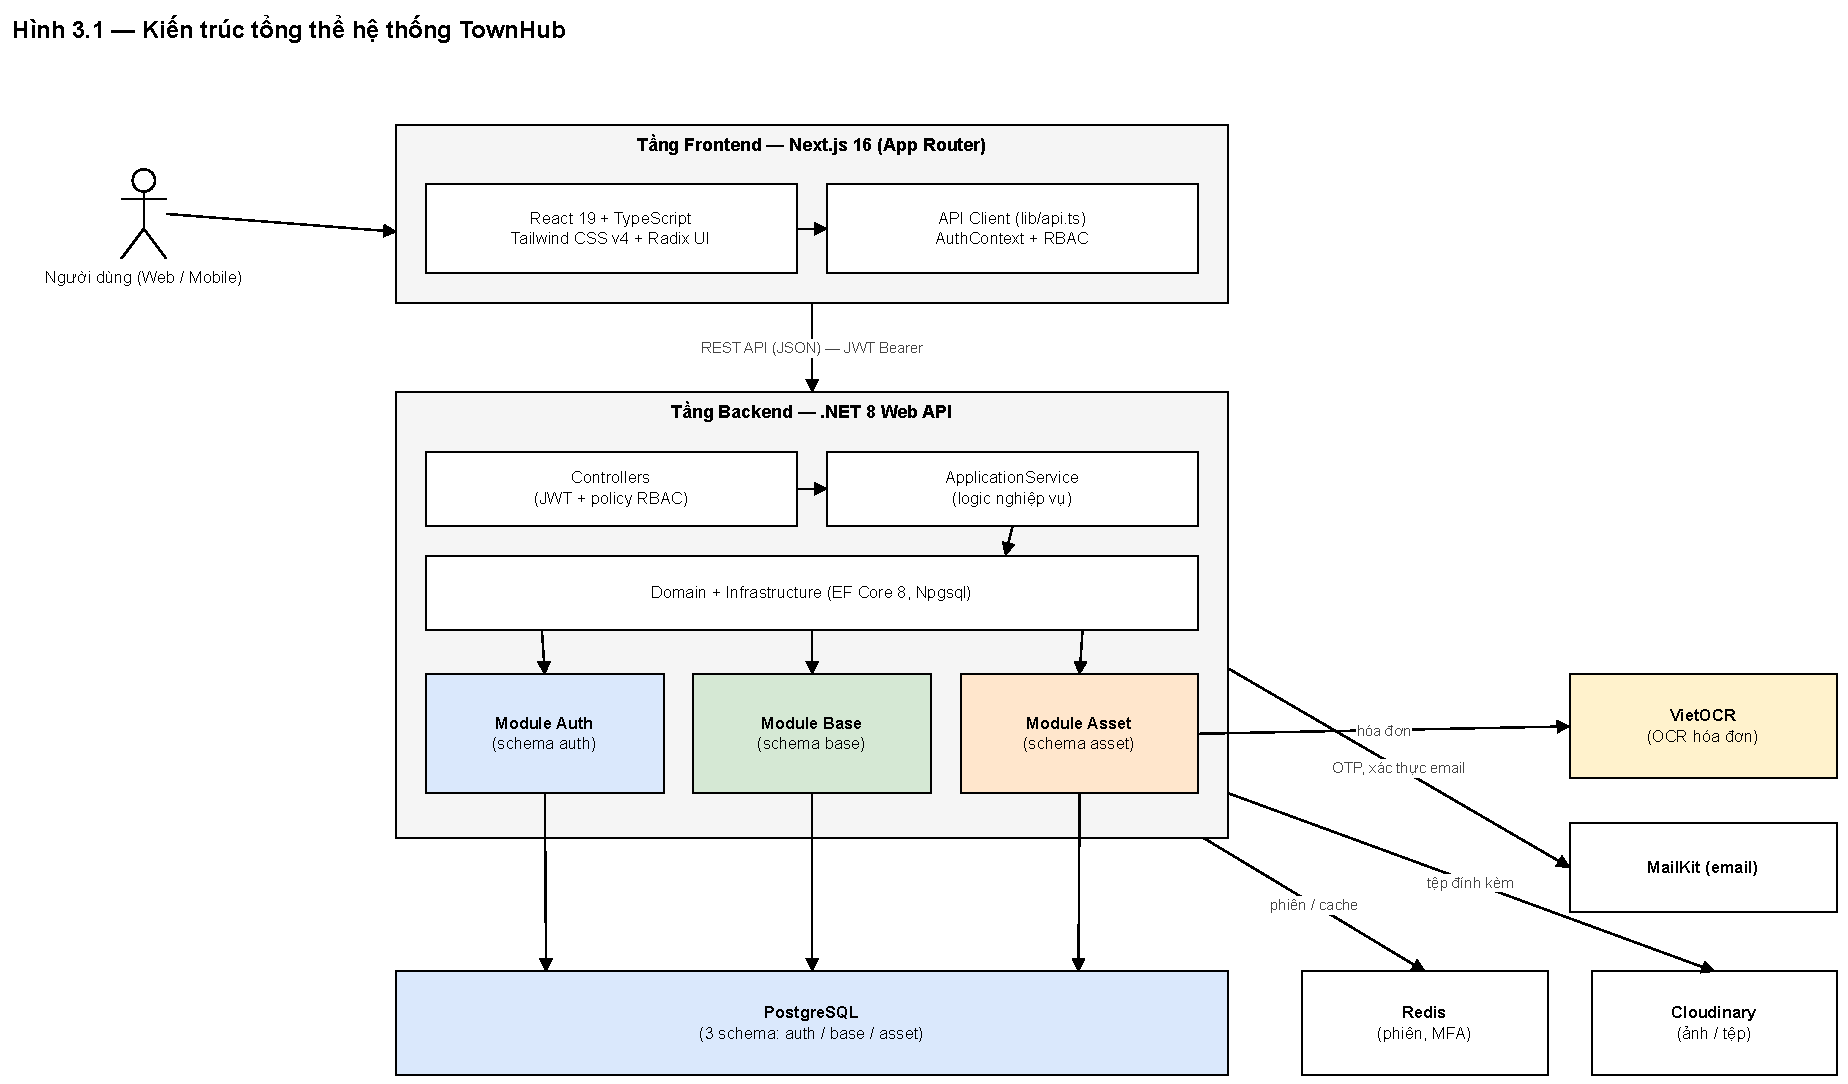
\includegraphics[width=\linewidth,height=0.82\textheight,keepaspectratio]{images/img06.pdf}
\caption*{\small Hình 3.1. Kiến trúc tổng thể hệ thống TownHub}
\addcontentsline{lof}{figure}{Hình 3.1. Kiến trúc tổng thể hệ thống TownHub}
\end{figure}
Tầng Frontend được phát triển bằng Next.js 16 (App Router) và React 19, sử dụng TypeScript, Tailwind CSS v4 và bộ component Radix UI; toàn bộ lời gọi API tập trung ở tầng client (lib/api.ts) và tự động gắn token xác thực vào mỗi yêu cầu.

Tầng Backend là ứng dụng .NET 8 Web API tổ chức theo kiến trúc phân tầng: Controllers tiếp nhận yêu cầu và kiểm tra quyền $\rightarrow$ ApplicationService xử lý logic nghiệp vụ $\rightarrow$ Domain (thực thể) và Infrastructure (EF Core 8, Npgsql) truy cập dữ liệu. Backend được chia thành ba module độc lập là Auth, Base và Asset, tương ứng ba nhóm nghiệp vụ và ba schema cơ sở dữ liệu.

Tầng dữ liệu và dịch vụ ngoài gồm: PostgreSQL (ba schema auth/asset/base) làm CSDL chính; Redis lưu phiên và trạng thái MFA; Cloudinary lưu ảnh/tệp; VietOCR và MailKit phục vụ nhận dạng hóa đơn và gửi email. Mọi API trả về theo cấu trúc thống nhất ResponseDto<T> gồm ErrorCode, ErrorMessage và Data, giúp frontend xử lý phản hồi nhất quán.

\phantomsection
\section*{3.2. Biểu đồ Use Case tổng quát}
\addcontentsline{toc}{section}{3.2. Biểu đồ Use Case tổng quát}
Các phân hệ Base phục vụ nhiều nhóm người dùng với vai trò khác nhau. Biểu đồ use case tổng quát của module Base được thể hiện ở Hình 3.2, mô tả các chức năng dùng chung và mối quan hệ với từng tác nhân.

\begin{figure}[H]\centering
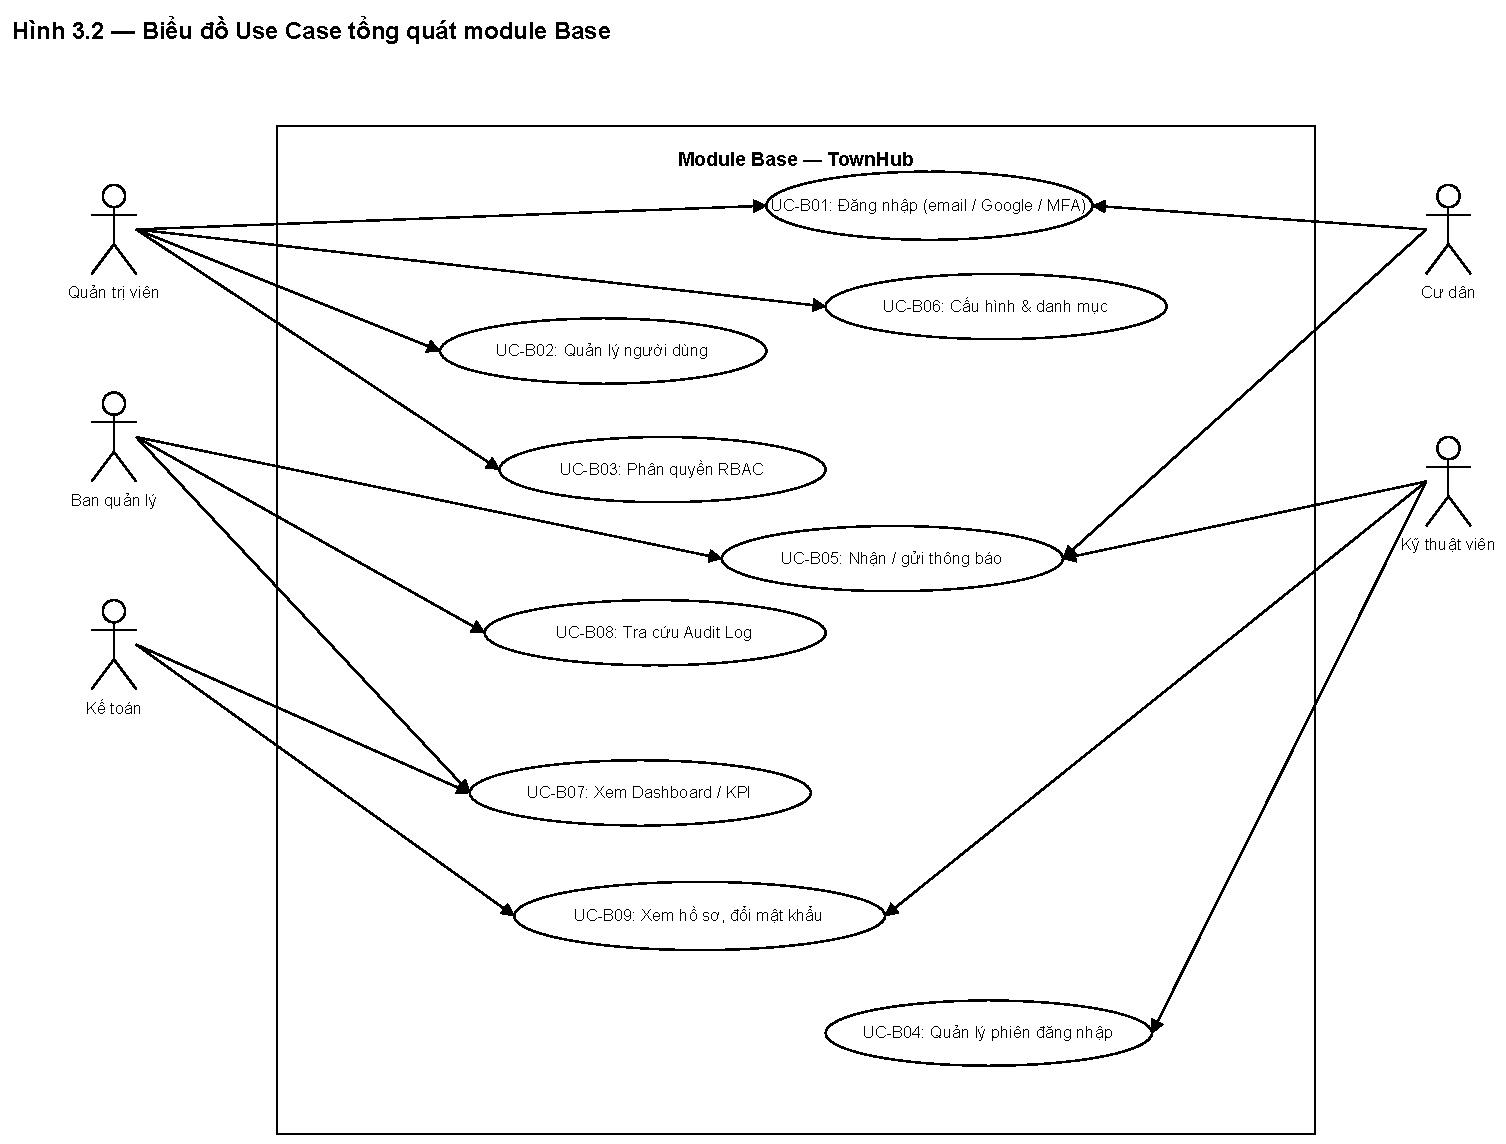
\includegraphics[width=\linewidth,height=0.82\textheight,keepaspectratio]{images/img07.pdf}
\caption*{\small Hình 3.2. Biểu đồ Use Case tổng quát module Base}
\addcontentsline{lof}{figure}{Hình 3.2. Biểu đồ Use Case tổng quát module Base}
\end{figure}
Các tác nhân chính của hệ thống:

\begin{center}{\singlespacing\renewcommand{\arraystretch}{1.25}
\begin{tabular}{|>{\raggedright\arraybackslash}p{\dimexpr\linewidth/2-2\tabcolsep-\arrayrulewidth\relax}|>{\raggedright\arraybackslash}p{\dimexpr\linewidth/2-2\tabcolsep-\arrayrulewidth\relax}|}
\hline
\textbf{Tác nhân} & \textbf{Mô tả vai trò} \\ \hline
Quản trị viên & Cấu hình hệ thống, quản lý tài khoản, phân quyền; toàn quyền hệ thống. \\ \hline
Ban quản lý & Theo dõi vận hành, xem báo cáo, nhận và xử lý thông báo. \\ \hline
Kế toán & Nghiệp vụ tài chính (tài sản, chi phí), xem báo cáo. \\ \hline
Cư dân & Đăng nhập, nhận thông báo, gửi yêu cầu/​sự cố. \\ \hline
Kỹ thuật viên & Đăng nhập, nhận việc/​thông báo, cập nhật xử lý. \\ \hline
\end{tabular}}\end{center}
\phantomsection
\section*{3.3. Thiết kế cơ sở dữ liệu lõi (schema auth)}
\addcontentsline{toc}{section}{3.3. Thiết kế cơ sở dữ liệu lõi (schema auth)}
Cơ sở dữ liệu lõi của Base tập trung ở schema auth, quản lý người dùng, phân quyền theo vai trò (RBAC), phiên đăng nhập và nhật ký hoạt động. Sơ đồ thực thể – liên kết (ERD) được trình bày ở Hình 3.3.

\begin{figure}[H]\centering
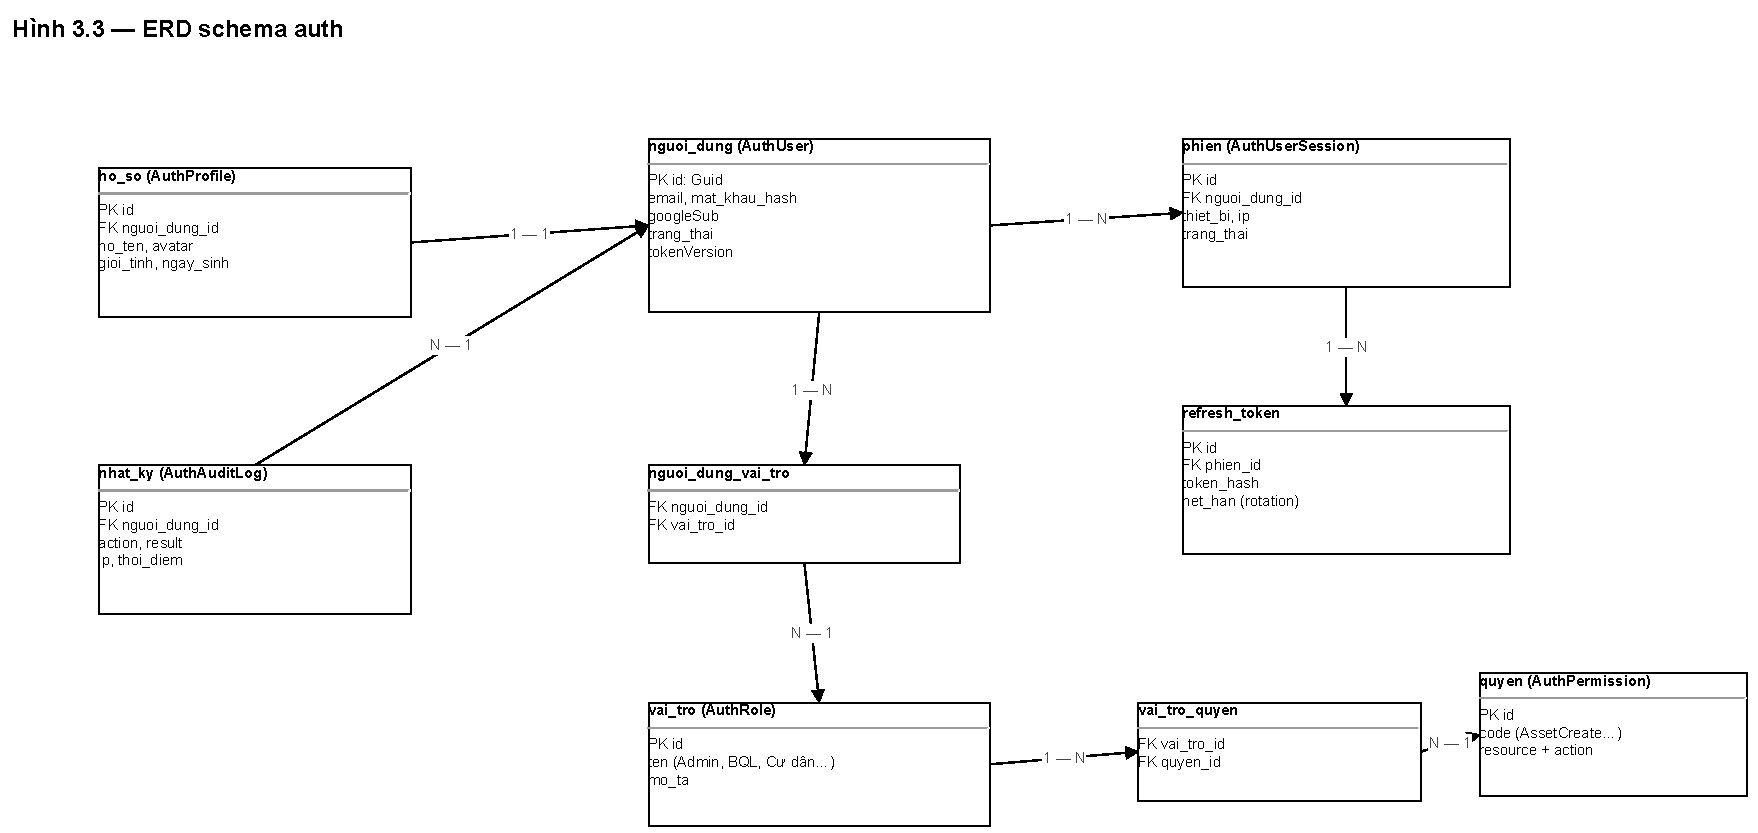
\includegraphics[width=\linewidth,height=0.82\textheight,keepaspectratio]{images/img08.pdf}
\caption*{\small Hình 3.3. Sơ đồ thực thể – liên kết (ERD) schema auth}
\addcontentsline{lof}{figure}{Hình 3.3. Sơ đồ thực thể – liên kết (ERD) schema auth}
\end{figure}
Các thực thể chính và quan hệ:

\begin{center}{\singlespacing\renewcommand{\arraystretch}{1.25}
\begin{tabular}{|>{\raggedright\arraybackslash}p{\dimexpr\linewidth/3-2\tabcolsep-\arrayrulewidth\relax}|>{\raggedright\arraybackslash}p{\dimexpr\linewidth/3-2\tabcolsep-\arrayrulewidth\relax}|>{\raggedright\arraybackslash}p{\dimexpr\linewidth/3-2\tabcolsep-\arrayrulewidth\relax}|}
\hline
\textbf{Thực thể} & \textbf{Ý nghĩa} & \textbf{Quan hệ chính} \\ \hline
nguoi\_dung (AuthUser) & Tài khoản: email, mật khẩu băm, googleSub, trạng thái, tokenVersion & 1–1 ho\_so; 1–N phiên, nhật ký \\ \hline
ho\_so (AuthProfile) & Hồ sơ cá nhân: họ tên, avatar, giới tính\ldots{} & Thuộc một người dùng \\ \hline
vai\_tro (AuthRole) & Vai trò (Admin, BQL, Cư dân, Kỹ thuật\ldots{}) & N–N người dùng; N–N quyền \\ \hline
quyen (AuthPermission) & Quyền chi tiết theo code (AssetCreate\ldots{}) & N–N vai trò \\ \hline
nguoi\_dung\_vai\_tro / vai\_tro\_quyen & Bảng nối gán vai trò $\leftrightarrow$ người dùng, quyền $\leftrightarrow$ vai trò & Bảng trung gian N–N \\ \hline
phien (AuthUserSession) & Phiên theo thiết bị (đa thiết bị) & 1–N refresh\_token \\ \hline
refresh\_token & Refresh token, hỗ trợ rotation & Thuộc một phiên \\ \hline
nhat\_ky (AuthAuditLog) & Nhật ký hành động: action, result, IP\ldots{} & Thuộc một người dùng \\ \hline
\end{tabular}}\end{center}
\phantomsection
\section*{3.4. Đặc tả các phân hệ Base}
\addcontentsline{toc}{section}{3.4. Đặc tả các phân hệ Base}
\phantomsection
\subsection*{3.4.1. Auth \& Security - Xác thực và phân quyền}
\addcontentsline{toc}{subsection}{3.4.1. Auth \& Security - Xác thực và phân quyền}
Phân hệ xác thực hỗ trợ ba phương thức đăng nhập: email/mật khẩu, đăng nhập Google (OAuth 2.0) và luồng riêng cho ứng dụng di động (trả token trong nội dung phản hồi thay vì cookie). Sau khi xác thực thành công, hệ thống cấp AccessToken (hiệu lực khoảng 30 phút) và RefreshToken (khoảng 7 ngày); áp dụng token rotation và trường tokenVersion để vô hiệu hóa token khi cần. Với giao diện web, token được lưu trong cookie HttpOnly kèm CSRF token; hệ thống quản lý phiên theo từng thiết bị, cho phép đăng xuất trên một hoặc tất cả thiết bị.

Để tăng cường bảo mật, hệ thống hỗ trợ xác thực đa yếu tố (MFA) bằng mã OTP theo thời gian (TOTP, thư viện Otp.NET) qua ứng dụng authenticator, cùng chức năng xác thực email và đặt lại mật khẩu qua email (MailKit). Luồng đăng nhập có MFA và cấp JWT được minh họa ở Hình 3.4.

\begin{figure}[H]\centering
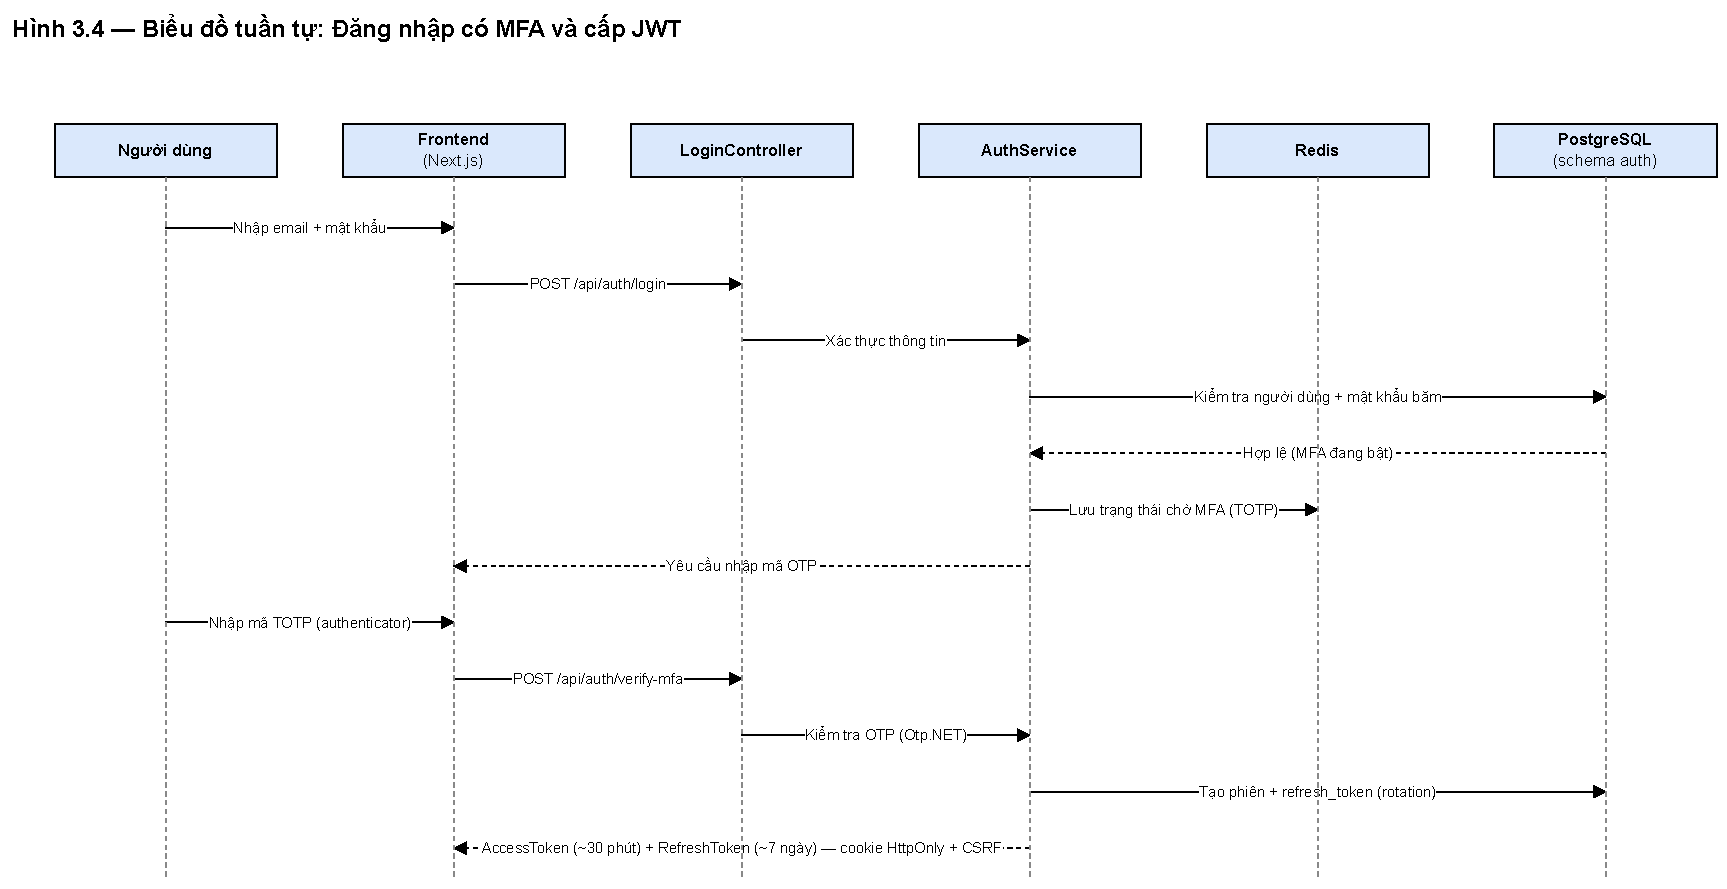
\includegraphics[width=\linewidth,height=0.82\textheight,keepaspectratio]{images/img09.pdf}
\caption*{\small Hình 3.4. Biểu đồ tuần tự: Đăng nhập có MFA và cấp JWT}
\addcontentsline{lof}{figure}{Hình 3.4. Biểu đồ tuần tự: Đăng nhập có MFA và cấp JWT}
\end{figure}
Giao diện màn hình đăng nhập thực tế của hệ thống được thể hiện ở Hình 3.5.

\begin{figure}[H]\centering
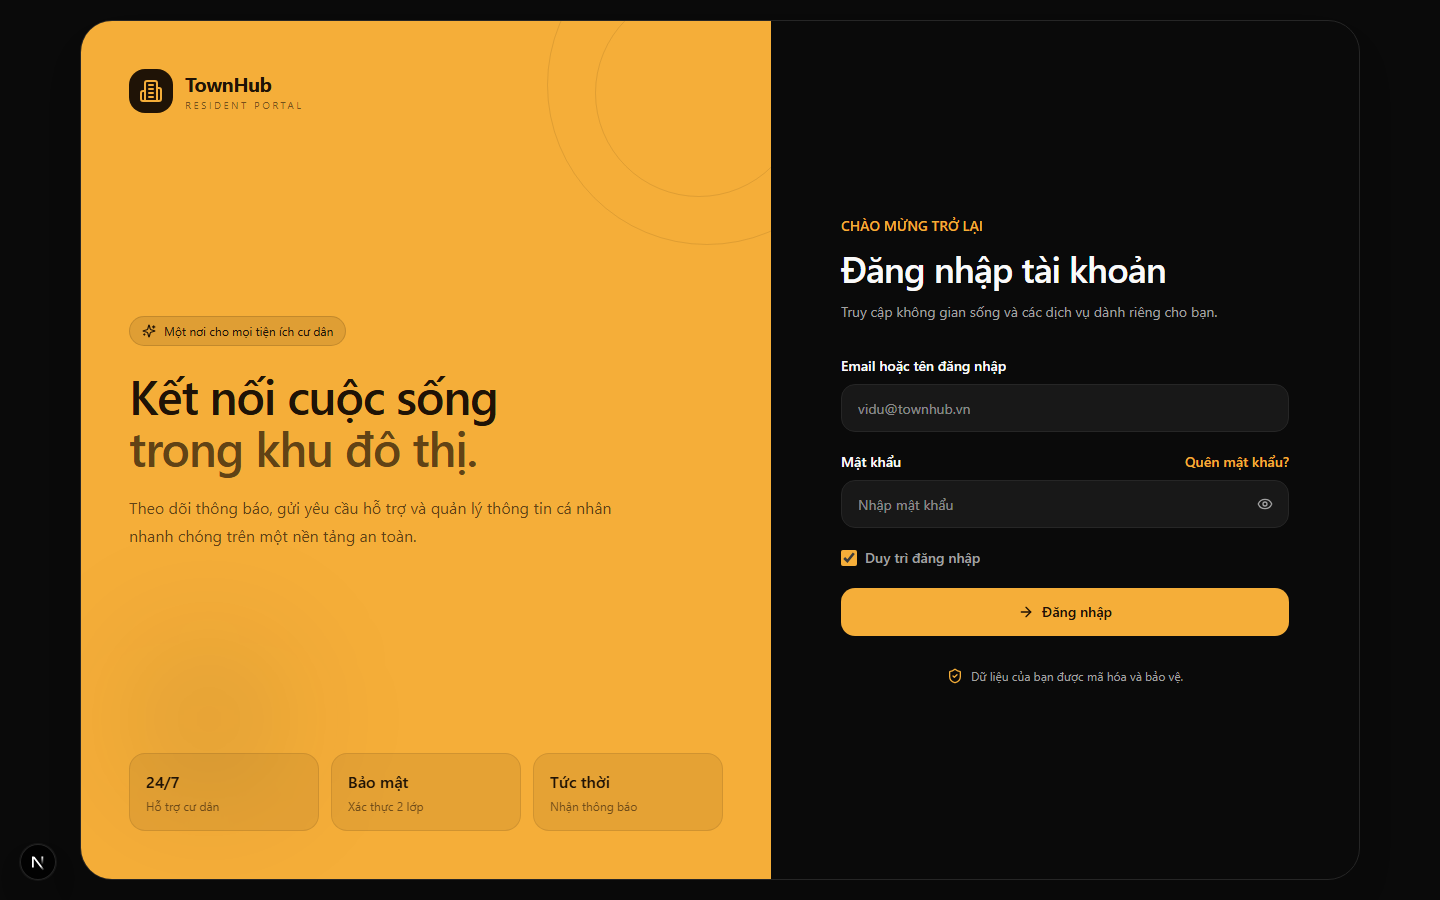
\includegraphics[width=\linewidth,height=0.82\textheight,keepaspectratio]{images/img10.png}
\caption*{\small Hình 3.5. Giao diện màn hình đăng nhập}
\addcontentsline{lof}{figure}{Hình 3.5. Giao diện màn hình đăng nhập}
\end{figure}
Về phân quyền, hệ thống áp dụng RBAC: quyền được định nghĩa chi tiết theo cặp resource + action (ví dụ AssetCreate, AssetUpdate, AccountMfaSetup\ldots{}) và gán cho vai trò; vai trò gán cho người dùng. Các controller chính: LoginController, RegisterController, AccountController (xác thực); RoleController, PermissionController, RolePermissionController, UserRoleController (phân quyền); UserSessionController (quản lý phiên).

\phantomsection
\subsection*{3.4.2. User Management - Người dùng và nhật ký hoạt động}
\addcontentsline{toc}{subsection}{3.4.2. User Management - Người dùng và nhật ký hoạt động}
Phân hệ quản lý người dùng cung cấp các thao tác CRUD tài khoản (UserController) kèm trạng thái hoạt động, vai trò và thông tin hồ sơ. Base cung cấp định danh trung tâm để các phân hệ khác liên kết (ví dụ phân hệ Quản lý dân cư gắn tài khoản với cư dân/căn hộ). Toàn bộ hành động quan trọng trong hệ thống được ghi lại qua AuditLogController (đăng nhập, thay đổi quyền, thao tác dữ liệu\ldots{}) phục vụ truy vết và an toàn thông tin.

\phantomsection
\subsection*{3.4.3. Notification Engine - Thông báo}
\addcontentsline{toc}{subsection}{3.4.3. Notification Engine - Thông báo}
Phân hệ thông báo cho phép gửi thông báo đa kênh (push, email, SMS) qua NotificationController, quản lý mẫu thông báo tái sử dụng qua NotificationTemplateController và tra cứu lịch sử thông báo đã gửi. Đây là dịch vụ dùng chung cho các phân hệ nghiệp vụ, ví dụ cảnh báo tồn kho thấp, nhắc hạn bảo trì hoặc cảnh báo sắp/đã quá hạn SLA.

\phantomsection
\subsection*{3.4.4. Configuration - Cấu hình và danh mục dùng chung}
\addcontentsline{toc}{subsection}{3.4.4. Configuration - Cấu hình và danh mục dùng chung}
Phân hệ cấu hình quản lý các tham số chung của hệ thống (tên khu, logo, định dạng và độ dài sinh mã, phương pháp khấu hao mặc định\ldots{}) và các danh mục dùng chung như loại tài sản, loại phí, loại dịch vụ. Việc tập trung danh mục giúp chuẩn hóa dữ liệu đầu vào và cho phép các phân hệ tự động áp dụng giá trị mặc định.

\phantomsection
\subsection*{3.4.5. Reporting - Dashboard và KPI}
\addcontentsline{toc}{subsection}{3.4.5. Reporting - Dashboard và KPI}
Phân hệ báo cáo tổng hợp số liệu toàn hệ thống thành dashboard trực quan và các báo cáo KPI, báo cáo chi phí (route /reports, /reports/kpi, /reports/cost; KpiSnapshotController, CostTrackingController). Số liệu được thu thập từ các phân hệ nghiệp vụ để phục vụ ra quyết định vận hành. Giao diện Bảng điều khiển được thể hiện ở Hình 3.6.

\begin{figure}[H]\centering
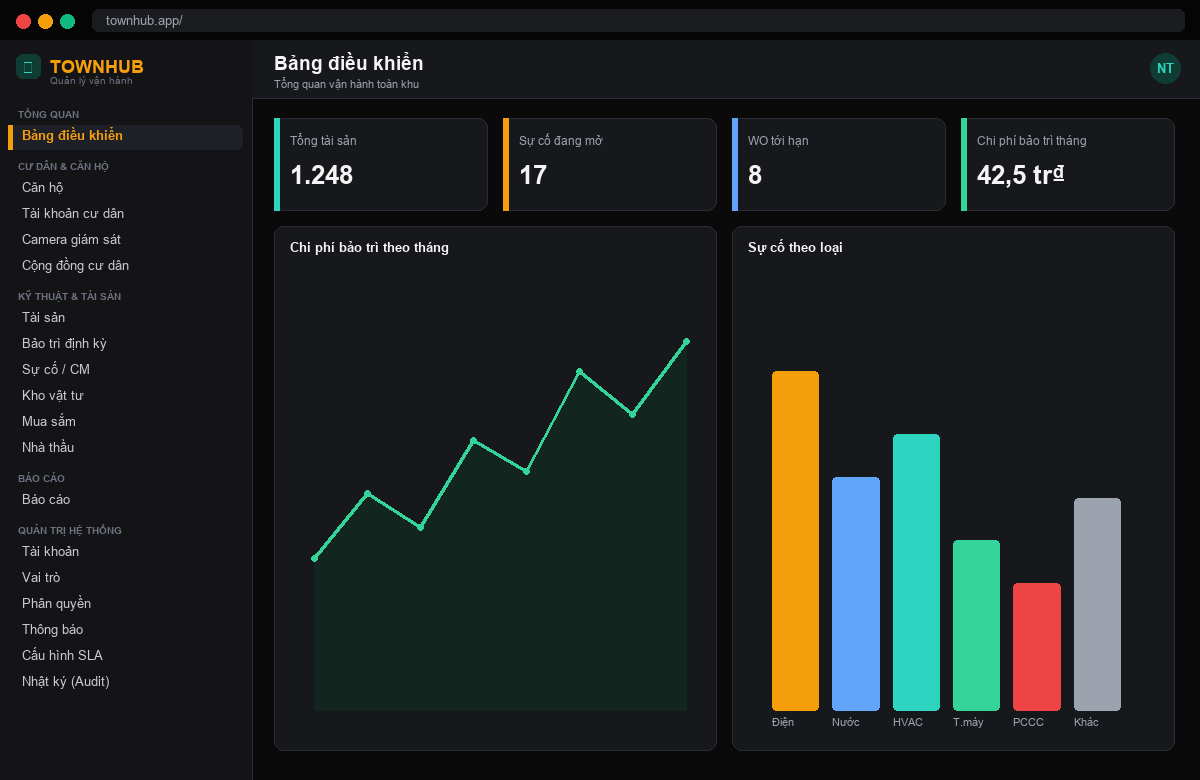
\includegraphics[width=\linewidth,height=0.82\textheight,keepaspectratio]{images/img11.png}
\caption*{\small Hình 3.6. Giao diện Bảng điều khiển (Dashboard) tổng quan}
\addcontentsline{lof}{figure}{Hình 3.6. Giao diện Bảng điều khiển (Dashboard) tổng quan}
\end{figure}
\phantomsection
\section*{3.5. Thiết kế API dùng chung và điểm mở rộng cho phân hệ riêng}
\addcontentsline{toc}{section}{3.5. Thiết kế API dùng chung và điểm mở rộng cho phân hệ riêng}
Base định ra các quy ước kỹ thuật để các phân hệ riêng tích hợp đồng nhất:

\begin{itemize}[leftmargin=1.4em,itemsep=1pt,topsep=2pt]
  \item Mọi API trả về cấu trúc ResponseDto<T> \{ ErrorCode, ErrorMessage, Data \} để chuẩn hóa xử lý phản hồi và lỗi.
  \item Mọi endpoint yêu cầu xác thực JWT và kiểm tra quyền bằng policy RBAC gắn ở controller.
  \item Các phân hệ tham chiếu định danh cross-service bằng Guid (ví dụ buildingId, floorId của Base; createdBy, assignedTo của Auth) và KHÔNG dùng navigation property xuyên module, giữ cho ba module độc lập, dễ bảo trì và triển khai.
  \item Thông báo, audit log, cấu hình và danh mục được cung cấp dưới dạng dịch vụ dùng lại cho mọi phân hệ.
\end{itemize}
\phantomsection
\section*{3.6. Kết luận chương}
\addcontentsline{toc}{section}{3.6. Kết luận chương}
Chương 3 đã trình bày kiến trúc tổng thể, biểu đồ use case, thiết kế cơ sở dữ liệu lõi (schema auth) và đặc tả năm phân hệ Base (Auth \& Security, User Management, Notification Engine, Configuration, Reporting) cùng các quy ước tích hợp. Đây là nền tảng để các phân hệ nghiệp vụ - trong đó có phân hệ Quản lý tài sản do tác giả đảm nhiệm - được xây dựng ở các chương tiếp theo.

\phantomsection
\chapter*{Chương 4. Phân tích và thiết kế phân hệ Quản lý tài sản (phần riêng)}
\addcontentsline{toc}{chapter}{Chương 4. Phân tích và thiết kế phân hệ Quản lý tài sản (phần riêng)}
\markboth{Chương 4. Phân tích và thiết kế phân hệ Quản lý tài sản (phần riêng)}{Chương 4. Phân tích và thiết kế phân hệ Quản lý tài sản (phần riêng)}
\textbf{Sinh viên thực hiện: }Nguyễn Xuân Thưởng   –   MSSV: 0220766   –   Lớp: 66KSCS

Chương này trình bày phân tích và thiết kế phân hệ Quản lý tài sản do tác giả (Nguyễn Xuân Thưởng) đảm nhiệm, gồm ba nghiệp vụ liên thông: (4.1) Tài sản \& bảo trì, (4.2) Kho – Mua sắm – Nhà cung cấp, (4.3) Sự cố \& SLA. Cả ba đều thuộc module Asset ở backend và kế thừa các dịch vụ nền tảng của module Base (Chương 3). Hai phân hệ Quản lý dân cư (Lương Thanh Tài) và Quản lý dịch vụ (Nguyễn Xuân Khải) do các thành viên khác trong nhóm đảm nhiệm và không thuộc phạm vi trình bày của báo cáo này.

\phantomsection
\section*{4.1. Nghiệp vụ Tài sản \& bảo trì}
\addcontentsline{toc}{section}{4.1. Nghiệp vụ Tài sản \& bảo trì}
\phantomsection
\subsection*{4.1.1. Đặt vấn đề và phạm vi}
\addcontentsline{toc}{subsection}{4.1.1. Đặt vấn đề và phạm vi}
Một tòa nhà sở hữu số lượng lớn tài sản cố định và thiết bị kỹ thuật. Quản lý thủ công dẫn tới khó tra cứu, không theo dõi được vòng đời và giá trị còn lại, tính khấu hao sai lệch, bỏ sót lịch bảo trì, số liệu quản lý vật lý không khớp sổ kế toán.

Nghiệp vụ Tài sản \& bảo trì là lõi nghiệp vụ của TownHub, quản lý toàn bộ vòng đời tài sản: ghi tăng (mua sắm) $\rightarrow$ cấp phát – điều chuyển $\rightarrow$ khấu hao định kỳ $\rightarrow$ bảo trì $\rightarrow$ thanh lý; mỗi biến động đều sinh chứng từ kế toán. Phần vận hành kỹ thuật (bảo trì phòng ngừa PM/Work Order) bảo đảm thiết bị được bảo dưỡng đúng hạn.

\begin{itemize}[leftmargin=1.4em,itemsep=1pt,topsep=2pt]
  \item Quản lý danh mục tài sản, vị trí lắp đặt và mã QR cho từng tài sản.
  \item Ghi tăng tài sản (đơn lẻ hoặc theo lô) và tự sinh mã theo cấu hình.
  \item Cấp phát, thu hồi, luân chuyển tài sản giữa phòng ban và người dùng.
  \item Tính và ghi nhận khấu hao (đường thẳng, số dư giảm dần, tổng số năm).
  \item Bảo trì phòng ngừa theo lịch (Work Order, checklist, check-in kỹ thuật viên).
  \item Thanh lý tài sản, tính lãi/lỗ; tự động sinh chứng từ và bút toán Nợ/Có.
\end{itemize}
\phantomsection
\subsection*{4.1.2. Mối liên hệ và kế thừa từ module Base}
\addcontentsline{toc}{subsection}{4.1.2. Mối liên hệ và kế thừa từ module Base}
Theo nguyên tắc phân chia module độc lập nhưng liên thông mà nhóm thống nhất, phân hệ không xây dựng lại các dịch vụ nền tảng mà kế thừa trực tiếp thành quả chung từ module Base:

\begin{itemize}[leftmargin=1.4em,itemsep=1pt,topsep=2pt]
  \item \textbf{Auth/RBAC: }mọi API yêu cầu JWT; policy AssetView, AssetCreate, AssetUpdate, AssetDelete gắn ở controller.
  \item \textbf{Định danh không gian (Base): }tài sản/vị trí tham chiếu buildingId, floorId dạng Guid cross-service.
  \item \textbf{Configuration: }định dạng sinh mã, phương pháp khấu hao mặc định, danh mục loại tài sản/tài khoản kế toán.
  \item \textbf{Notification \& Reporting: }cảnh báo hạn bảo trì/quá hạn; số liệu giá trị \& chi phí đẩy lên Dashboard/KPI.
\end{itemize}
\phantomsection
\subsection*{4.1.3. Phân tích yêu cầu chức năng}
\addcontentsline{toc}{subsection}{4.1.3. Phân tích yêu cầu chức năng}
Các tác nhân chính:

\begin{center}{\singlespacing\renewcommand{\arraystretch}{1.25}
\begin{tabular}{|>{\raggedright\arraybackslash}p{\dimexpr\linewidth/2-2\tabcolsep-\arrayrulewidth\relax}|>{\raggedright\arraybackslash}p{\dimexpr\linewidth/2-2\tabcolsep-\arrayrulewidth\relax}|}
\hline
\textbf{Tác nhân} & \textbf{Vai trò} \\ \hline
Quản trị viên & Cấu hình, danh mục, phân quyền. \\ \hline
Kế toán & Ghi tăng, khấu hao, thanh lý, đối chiếu chứng từ. \\ \hline
Quản lý / BQL & Duyệt điều chuyển, theo dõi giá trị \& tình trạng. \\ \hline
Kỹ thuật viên & Cấp phát, kiểm kê, quét QR, thực hiện Work Order bảo trì. \\ \hline
\end{tabular}}\end{center}
\subsubsection*{a) Danh mục và vị trí tài sản}
Khai báo danh mục (mã, tên, tiền tố sinh mã, thời gian khấu hao mặc định, tài khoản hạch toán) và vị trí lắp đặt theo tòa nhà/tầng; dùng lại khi ghi tăng để chuẩn hóa dữ liệu.

\subsubsection*{b) Ghi tăng và vòng đời tài sản}
Nhập danh mục, tên, số seri, nhà sản xuất, thông số kỹ thuật (JSON), thông tin tài chính (nguyên giá, ngày mua, thời gian \& phương pháp khấu hao, giá trị thu hồi). Trạng thái: nhàn rỗi $\rightarrow$ đang sử dụng $\rightarrow$ đang bảo trì $\rightarrow$ đã thanh lý.

\subsubsection*{c) Mã QR tài sản}
Mỗi tài sản có mã QR sinh tự động; nhân viên quét QR bằng camera để mở nhanh trang chi tiết - hỗ trợ kiểm kê hiện trường.

\subsubsection*{d) Cấp phát, điều chuyển, thu hồi}
Chọn loại điều chuyển (cấp phát/thu hồi/luân chuyển), phòng ban/người nhận và nguồn; hệ thống tạo bản ghi điều chuyển, cập nhật phòng ban/người dùng và trạng thái; lịch sử hiển thị ở trang chi tiết.

\subsubsection*{e) Khấu hao định kỳ}
Đến kỳ (đầu tháng), hệ thống tính khấu hao theo phương pháp của từng tài sản, cộng dồn khấu hao lũy kế, trừ giá trị còn lại, ghi lịch sử khấu hao và sinh chứng từ. Ba phương pháp:

\begin{itemize}[leftmargin=1.4em,itemsep=1pt,topsep=2pt]
  \item \textbf{Đường thẳng: }khấu hao tháng = nguyên giá / thời gian khấu hao (số tháng).
  \item \textbf{Số dư giảm dần: }khấu hao nhanh giai đoạn đầu theo tỉ lệ trên giá trị còn lại.
  \item \textbf{Tổng số năm: }phân bổ theo tỉ trọng số năm sử dụng còn lại.
\end{itemize}
\subsubsection*{f) Bảo trì phòng ngừa (PM / Work Order)}
Luồng bảo trì: Lịch bảo trì định kỳ (chu kỳ, lead time) $\rightarrow$ tự sinh Work Order khi tới hạn $\rightarrow$ phân công kỹ thuật viên $\rightarrow$ check-in hiện trường $\rightarrow$ thực hiện checklist + đính kèm ảnh $\rightarrow$ nộp $\rightarrow$ nghiệm thu (duyệt/từ chối). Bảo trì có chi phí: sửa chữa hạch toán chi phí trong kỳ, nâng cấp cộng vào nguyên giá.

\subsubsection*{g) Thanh lý tài sản}
Tính giá trị còn lại từ nguyên giá và khấu hao lũy kế; nhập giá trị thu hồi; hệ thống tính lãi/lỗ, cập nhật trạng thái "đã thanh lý" và sinh chứng từ thanh lý.

\subsubsection*{h) Sổ kế toán và báo cáo tài chính tài sản}
Toàn bộ biến động tài sản (ghi tăng, khấu hao, thanh lý) đều sinh chứng từ kèm định khoản Nợ/Có; trên nền dữ liệu chứng từ đó, phân hệ cung cấp hệ thống sổ sách và báo cáo kế toán theo hình thức Nhật ký chung. Các sổ và báo cáo được dẫn xuất trực tiếp từ chứng từ nên luôn khớp sổ và tuân thủ hệ thống tài khoản theo Thông tư 200:

\begin{itemize}[leftmargin=1.4em,itemsep=1pt,topsep=2pt]
  \item \textbf{Nhật ký chung: }ghi nhận toàn bộ bút toán phát sinh theo trình tự thời gian, cho phép lọc theo khoảng thời gian và theo tài khoản.
  \item \textbf{Sổ cái: }theo dõi phát sinh Nợ/Có và số dư (đầu kỳ, trong kỳ, cuối kỳ) của từng tài khoản kế toán, kèm số dư lũy kế và tài khoản đối ứng của mỗi bút toán.
  \item \textbf{Bảng cân đối số phát sinh: }tổng hợp số dư đầu kỳ, phát sinh trong kỳ và số dư cuối kỳ của mọi tài khoản, đối chiếu cân đối tổng phát sinh Nợ bằng tổng phát sinh Có.
  \item \textbf{Sổ tài sản cố định: }liệt kê nguyên giá, hao mòn lũy kế và giá trị còn lại của từng tài sản (sổ chi tiết TSCĐ) kèm số liệu tổng hợp toàn danh mục.
  \item \textbf{Báo cáo tăng/giảm tài sản: }tổng hợp tài sản ghi tăng (mua mới) và ghi giảm (thanh lý) theo kỳ, kèm lãi/lỗ khi thanh lý.
\end{itemize}
\phantomsection
\subsection*{4.1.4. Yêu cầu phi chức năng}
\addcontentsline{toc}{subsection}{4.1.4. Yêu cầu phi chức năng}
\begin{itemize}[leftmargin=1.4em,itemsep=1pt,topsep=2pt]
  \item Bảo mật theo RBAC; dữ liệu tài chính chỉ hiển thị cho vai trò phù hợp.
  \item Toàn vẹn: mọi biến động sinh chứng từ; giao dịch nhiều bảng nhất quán.
  \item Hiệu năng: danh sách phân trang, lọc theo tòa nhà/danh mục/trạng thái.
\end{itemize}
\phantomsection
\subsection*{4.1.5. Thiết kế phân hệ}
\addcontentsline{toc}{subsection}{4.1.5. Thiết kế phân hệ}
\subsubsection*{a) Danh sách Use Case chính}
Các use case chính của phân hệ được thể hiện trên biểu đồ use case ở Hình 4.1 và liệt kê trong bảng dưới đây.

\begin{figure}[H]\centering

\includegraphics[width=\linewidth,height=0.82\textheight,keepaspectratio]{images/img12.pdf}
\caption*{\small Hình 4.1. Biểu đồ Use Case – Quản lý tài sản \& bảo trì}
\addcontentsline{lof}{figure}{Hình 4.1. Biểu đồ Use Case – Quản lý tài sản \& bảo trì}
\end{figure}
\begin{center}{\singlespacing\renewcommand{\arraystretch}{1.25}
\begin{tabular}{|>{\raggedright\arraybackslash}p{\dimexpr\linewidth/3-2\tabcolsep-\arrayrulewidth\relax}|>{\raggedright\arraybackslash}p{\dimexpr\linewidth/3-2\tabcolsep-\arrayrulewidth\relax}|>{\raggedright\arraybackslash}p{\dimexpr\linewidth/3-2\tabcolsep-\arrayrulewidth\relax}|}
\hline
\textbf{Mã UC} & \textbf{Use case} & \textbf{Tác nhân} \\ \hline
UC-AS-01 & Quản lý danh mục \& vị trí tài sản & Admin/​Kế toán \\ \hline
UC-AS-02 & Ghi tăng tài sản (sinh mã + QR) & Kế toán \\ \hline
UC-AS-03 & Quét QR tra cứu tài sản & Kỹ thuật \\ \hline
UC-AS-04 & Điều chuyển / cấp phát / thu hồi & Quản lý/Kỹ thuật \\ \hline
UC-AS-05 & Tính \& ghi nhận khấu hao & Kế toán/​Hệ thống \\ \hline
UC-AS-06 & Lập lịch \& thực hiện Work Order bảo trì & Kỹ thuật \\ \hline
UC-AS-07 & Thanh lý tài sản (tính lãi/​lỗ) & Kế toán \\ \hline
UC-AS-08 & Xem sổ kế toán \& báo cáo tài chính & Kế toán/​Quản lý \\ \hline
\end{tabular}}\end{center}
\subsubsection*{b) Biểu đồ tuần tự và lưu đồ luồng tiêu biểu}
Luồng ghi tăng tài sản được minh họa ở Hình 4.2: người dùng nhập thông tin ở màn hình /assets $\rightarrow$ AssetController nhận POST create $\rightarrow$ AssetService kiểm tra dữ liệu và sinh mã (kiểm tra trùng), khởi tạo giá trị còn lại bằng nguyên giá $\rightarrow$ lưu tài sản $\rightarrow$ sinh mã QR và chứng từ ghi\_tang $\rightarrow$ trả ResponseDto về giao diện.

\begin{figure}[H]\centering

\includegraphics[width=\linewidth,height=0.82\textheight,keepaspectratio]{images/img13.pdf}
\caption*{\small Hình 4.2. Biểu đồ tuần tự: Ghi tăng tài sản}
\addcontentsline{lof}{figure}{Hình 4.2. Biểu đồ tuần tự: Ghi tăng tài sản}
\end{figure}
Luồng khấu hao định kỳ được minh họa ở Hình 4.3: người quản lý chọn kỳ và bấm ``Chạy khấu hao kỳ''; hệ thống lấy các tài sản đủ điều kiện chưa trích trong kỳ, tính khấu hao đường thẳng, sinh một chứng từ khấu hao tổng kèm định khoản Nợ 642 / Có 2141 cho từng tài sản, ghi lịch sử khấu hao (trỏ tới chứng từ) và cập nhật khấu hao luỹ kế, giá trị còn lại trên tài sản. Lưu đồ cũng thể hiện hai nghiệp vụ kế toán còn lại: ghi tăng khi nhập tài sản (sinh chứng từ Nợ 211|213 / Có 111|112) và thanh lý (sinh chứng từ Nợ 2141+811 / Có 211, đổi trạng thái tài sản sang DISPOSED) lũy kế và giá trị còn lại, ghi lich\_su\_khau\_hao và sinh chứng từ (Nợ 627 / Có 214), lặp cho đến khi xử lý hết.

\begin{figure}[H]\centering
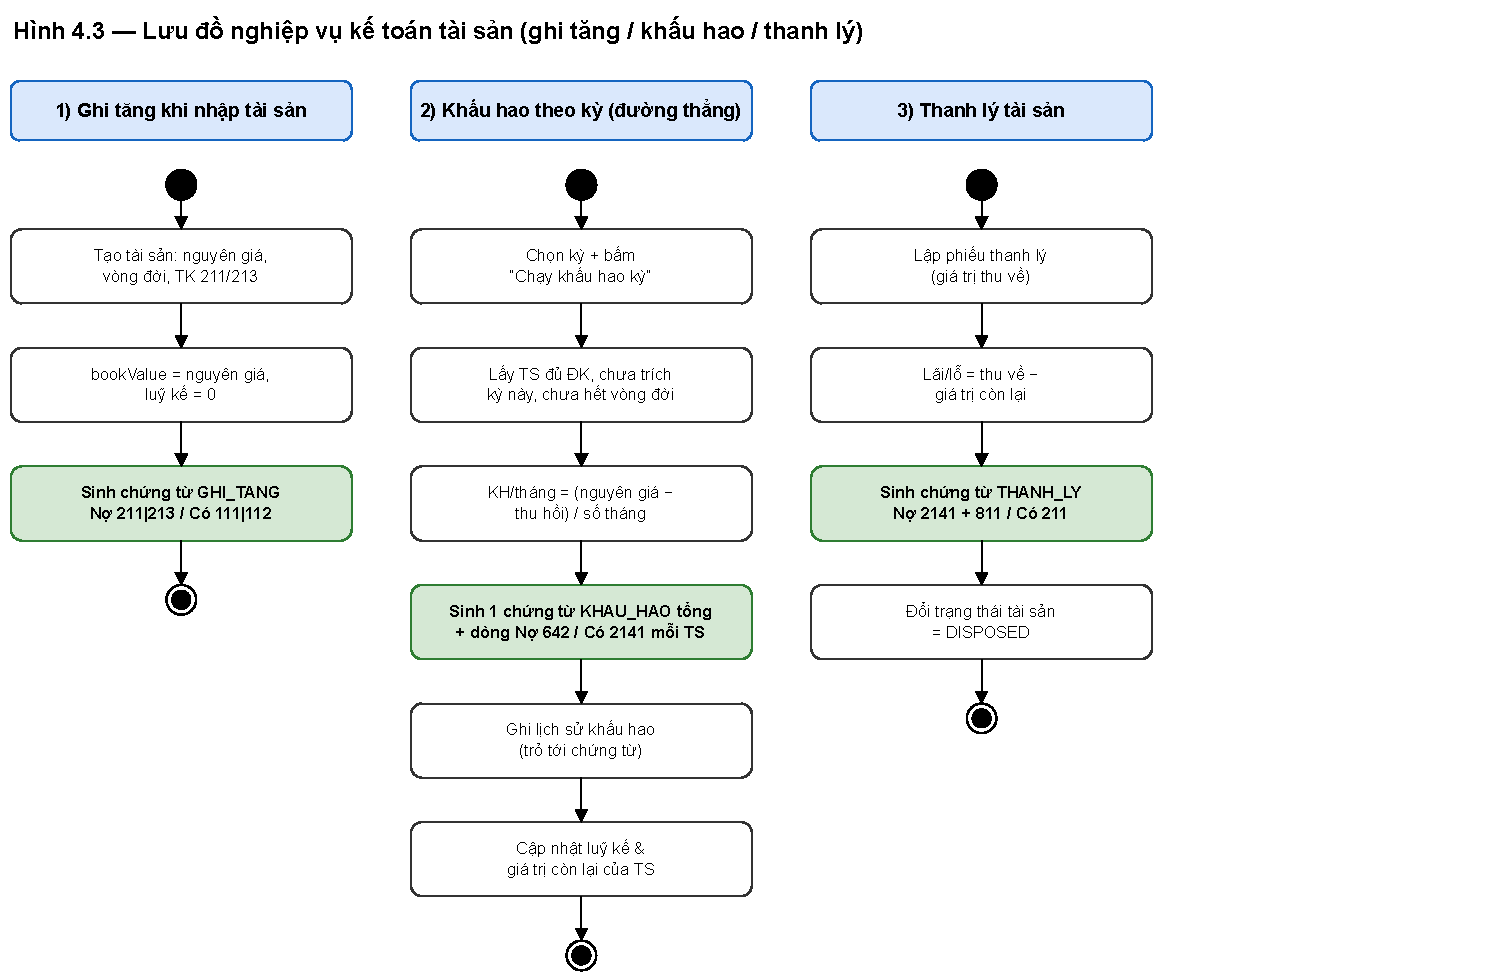
\includegraphics[width=\linewidth,height=0.82\textheight,keepaspectratio]{images/img14.pdf}
\caption*{\small Hình 4.3. Lưu đồ nghiệp vụ kế toán tài sản: ghi tăng – khấu hao – thanh lý}
\addcontentsline{lof}{figure}{Hình 4.3. Lưu đồ nghiệp vụ kế toán tài sản: ghi tăng – khấu hao – thanh lý}
\end{figure}
Với bảo trì phòng ngừa, quy trình khép kín từ tự động sinh Work Order khi tới hạn, phân công kỹ thuật viên, check-in bằng mã QR tại hiện trường, thực hiện checklist có ảnh minh chứng đến nghiệm thu được thể hiện ở Hình 4.4.

\begin{figure}[H]\centering

\includegraphics[width=\linewidth,height=0.82\textheight,keepaspectratio]{images/img15.pdf}
\caption*{\small Hình 4.4. Lưu đồ nghiệp vụ: Bảo trì định kỳ (PM/Work Order)}
\addcontentsline{lof}{figure}{Hình 4.4. Lưu đồ nghiệp vụ: Bảo trì định kỳ (PM/Work Order)}
\end{figure}
\subsubsection*{c) Thiết kế cơ sở dữ liệu (schema asset)}
Sơ đồ thực thể – liên kết của schema asset (Hình 4.5) lấy bảng tai\_san làm trung tâm, liên kết tới danh mục, lô, điều chuyển, bảo trì, thanh lý, lịch sử khấu hao và chứng từ kế toán.

\begin{figure}[H]\centering
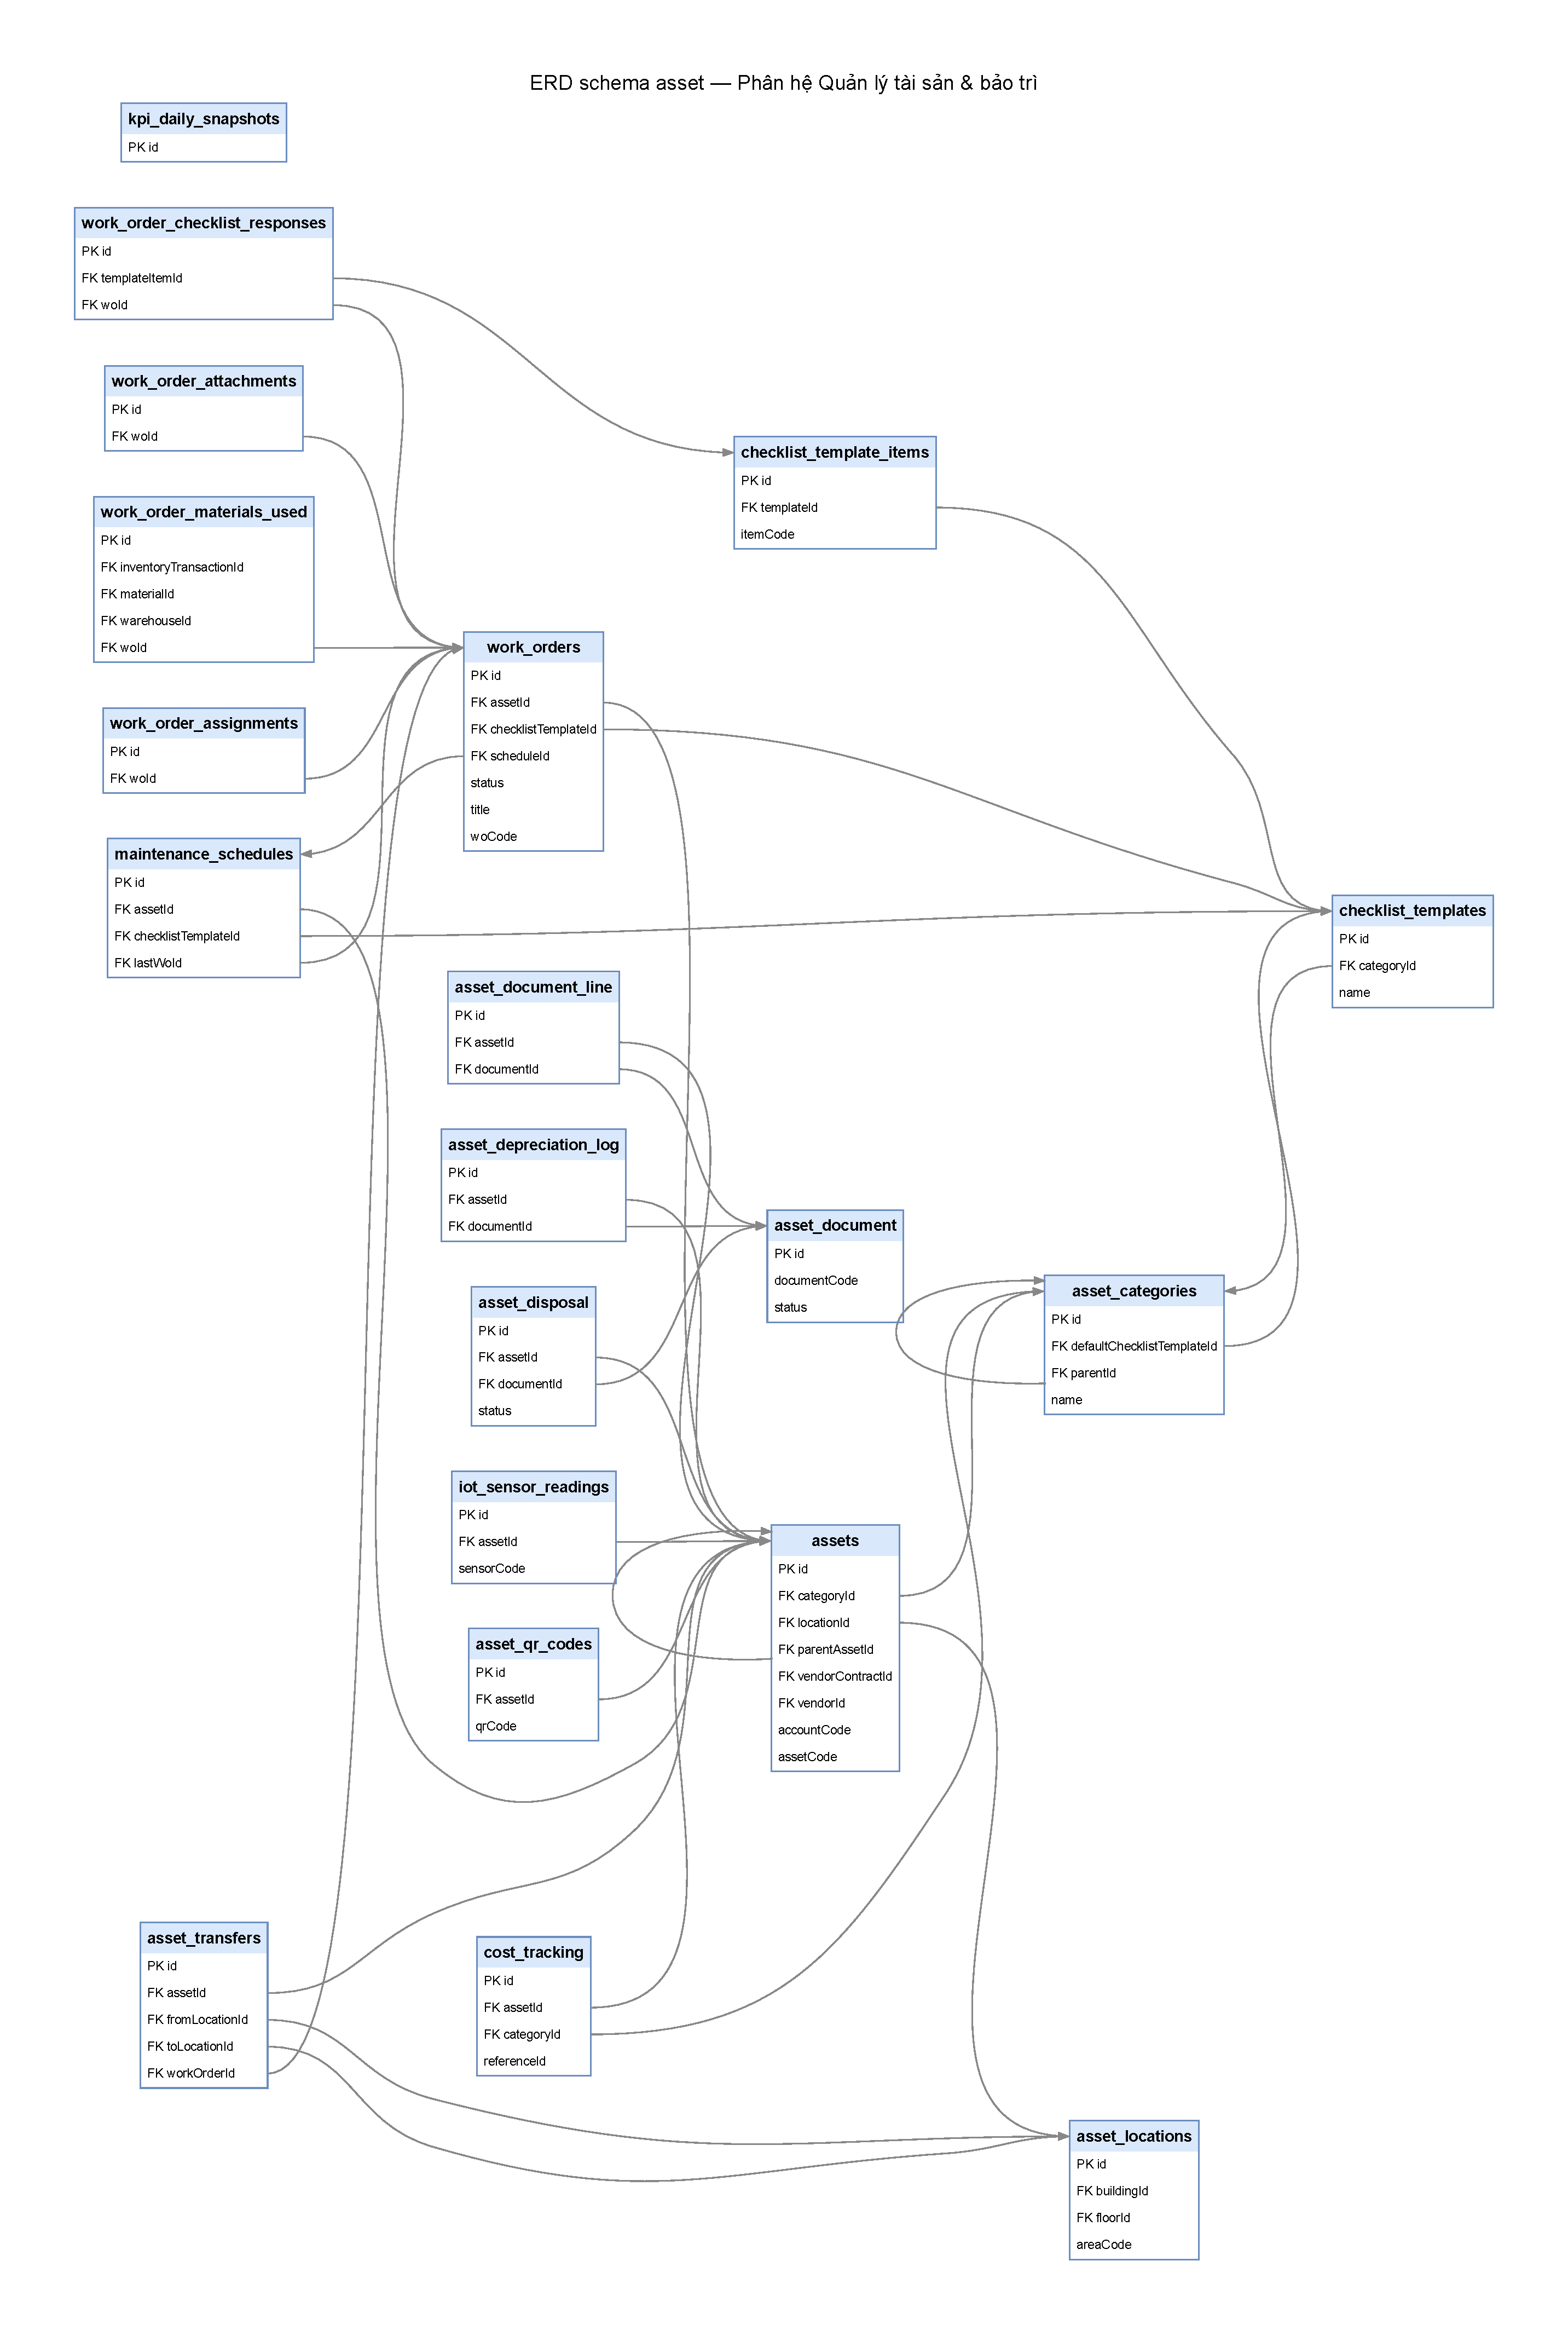
\includegraphics[width=\linewidth,height=0.9\textheight,keepaspectratio]{images/erd_asset.pdf}
\caption*{\small Hình 4.5. Sơ đồ thực thể – liên kết (ERD) schema asset}
\addcontentsline{lof}{figure}{Hình 4.5. Sơ đồ thực thể – liên kết (ERD) schema asset}
\end{figure}
\begin{center}{\singlespacing\renewcommand{\arraystretch}{1.25}
\begin{tabular}{|>{\raggedright\arraybackslash}p{\dimexpr\linewidth/3-2\tabcolsep-\arrayrulewidth\relax}|>{\raggedright\arraybackslash}p{\dimexpr\linewidth/3-2\tabcolsep-\arrayrulewidth\relax}|>{\raggedright\arraybackslash}p{\dimexpr\linewidth/3-2\tabcolsep-\arrayrulewidth\relax}|}
\hline
\textbf{Bảng} & \textbf{Ý nghĩa} & \textbf{Trường tiêu biểu} \\ \hline
tai\_san & Tài sản (trung tâm) & ma\_tai\_san, ten\_tai\_san, danh\_muc\_id, trang\_thai, nguyen\_gia, gia\_tri\_con\_lai, khau\_hao\_luy\_ke, phuong\_phap\_khau\_hao \\ \hline
danh\_muc\_tai\_san & Danh mục tài sản & ma\_danh\_muc, tien\_to, thoi\_gian\_khau\_hao, ma\_tai\_khoan \\ \hline
dieu\_chuyen\_tai\_san & Điều chuyển & loai\_dieu\_chuyen, tu/​den\_phong\_ban, tu/​den\_nguoi\_dung \\ \hline
bao\_tri\_tai\_san & Bảo trì & loai\_bao\_tri, chi\_phi, loai\_chi\_phi, trang\_thai \\ \hline
thanh\_ly\_tai\_san & Thanh lý & gia\_tri\_con\_lai, gia\_tri\_thanh\_ly, lai\_lo, ly\_do \\ \hline
lich\_su\_khau\_hao & Lịch sử khấu hao & ky\_khau\_hao, so\_tien, luy\_ke\_sau\_khau\_hao, con\_lai\_sau\_khau\_hao \\ \hline
MaintenanceSchedule / WorkOrder & Lịch bảo trì \& lệnh công việc & chu kỳ, lead time; trạng thái WO, phân công, checklist, đính kèm \\ \hline
chung\_tu / chi\_tiet\_chung\_tu & Chứng từ \& bút toán & loai\_chung\_tu; tai\_khoan\_no, tai\_khoan\_co, so\_tien \\ \hline
\end{tabular}}\end{center}
\subsubsection*{d) Thiết kế API và phân quyền}
\begin{center}{\singlespacing\renewcommand{\arraystretch}{1.25}
\begin{tabular}{|>{\raggedright\arraybackslash}p{\dimexpr\linewidth/3-2\tabcolsep-\arrayrulewidth\relax}|>{\raggedright\arraybackslash}p{\dimexpr\linewidth/3-2\tabcolsep-\arrayrulewidth\relax}|>{\raggedright\arraybackslash}p{\dimexpr\linewidth/3-2\tabcolsep-\arrayrulewidth\relax}|}
\hline
\textbf{Phương thức \& Endpoint} & \textbf{Chức năng} & \textbf{Quyền} \\ \hline
POST /api/​asset/​asset/​create & Ghi tăng tài sản & AssetCreate \\ \hline
GET /api/​asset/​asset/​get-all & Danh sách (lọc) & AssetView \\ \hline
/api/​asset/​asset-category/* & CRUD danh mục & Asset* \\ \hline
/api/​asset/​asset-qrcode/* & Sinh \& tra cứu QR & AssetView/​Create \\ \hline
/api/​asset/​asset-transfer/* & Điều chuyển tài sản & AssetUpdate \\ \hline
/api/​asset/​asset-depreciation/* & Tra cứu khấu hao & AssetView \\ \hline
/api/​asset/​asset-report/* & Nhật ký chung, sổ cái, báo cáo & AssetView \\ \hline
/api/​asset/​maintenance-schedule/* & Lịch bảo trì (get-overdue) & AssetView/​Update \\ \hline
/api/​asset/​work-order/* & Work Order (assign, checklist, attachment) & AssetView/​Update \\ \hline
\end{tabular}}\end{center}
\phantomsection
\subsection*{4.1.6. Thiết kế giao diện}
\addcontentsline{toc}{subsection}{4.1.6. Thiết kế giao diện}
\begin{center}{\singlespacing\renewcommand{\arraystretch}{1.25}
\begin{tabular}{|>{\raggedright\arraybackslash}p{\dimexpr\linewidth/2-2\tabcolsep-\arrayrulewidth\relax}|>{\raggedright\arraybackslash}p{\dimexpr\linewidth/2-2\tabcolsep-\arrayrulewidth\relax}|}
\hline
\textbf{Route} & \textbf{Chức năng} \\ \hline
/assets, /assets/[id] & Danh sách \& chi tiết tài sản \\ \hline
/assets/​scan & Quét QR tra cứu (jsqr) \\ \hline
/assets/​categories, /assets/​depreciation & Danh mục \& theo dõi khấu hao \\ \hline
/assets/​journal, /assets/​ledger, /assets/​reports & Nhật ký chung, sổ cái \& báo cáo kế toán \\ \hline
/pm/​work-orders, /pm/​schedules & Work Order \& lịch bảo trì (check-in, checklist, review) \\ \hline
\end{tabular}}\end{center}
Một số màn hình tiêu biểu của phân hệ:

\begin{figure}[H]\centering
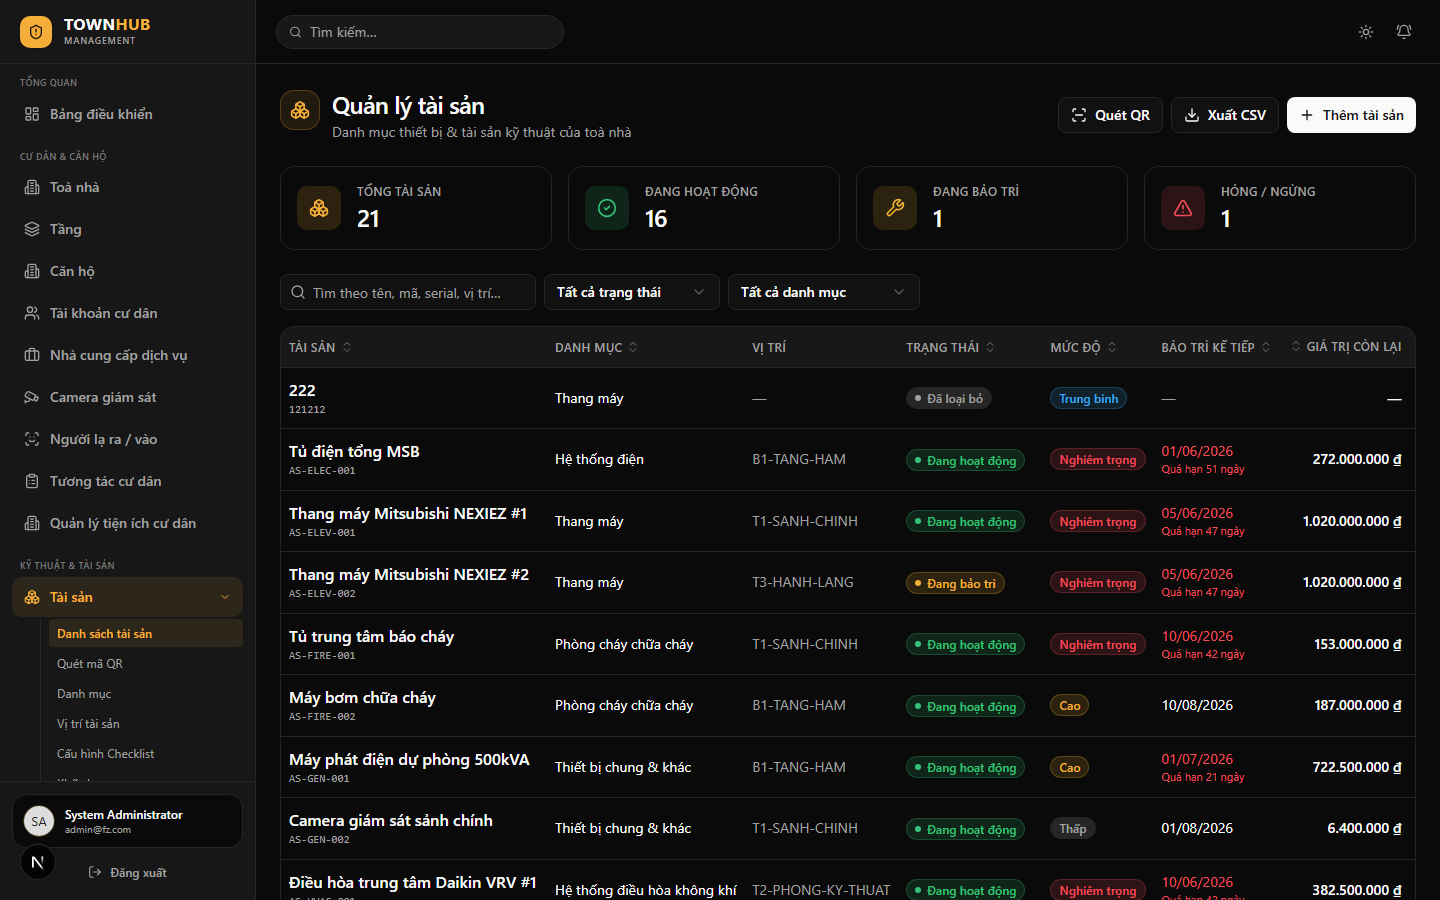
\includegraphics[width=\linewidth,height=0.82\textheight,keepaspectratio]{images/img17.png}
\caption*{\small Hình 4.6. Giao diện Danh sách tài sản}
\addcontentsline{lof}{figure}{Hình 4.6. Giao diện Danh sách tài sản}
\end{figure}
\begin{figure}[H]\centering
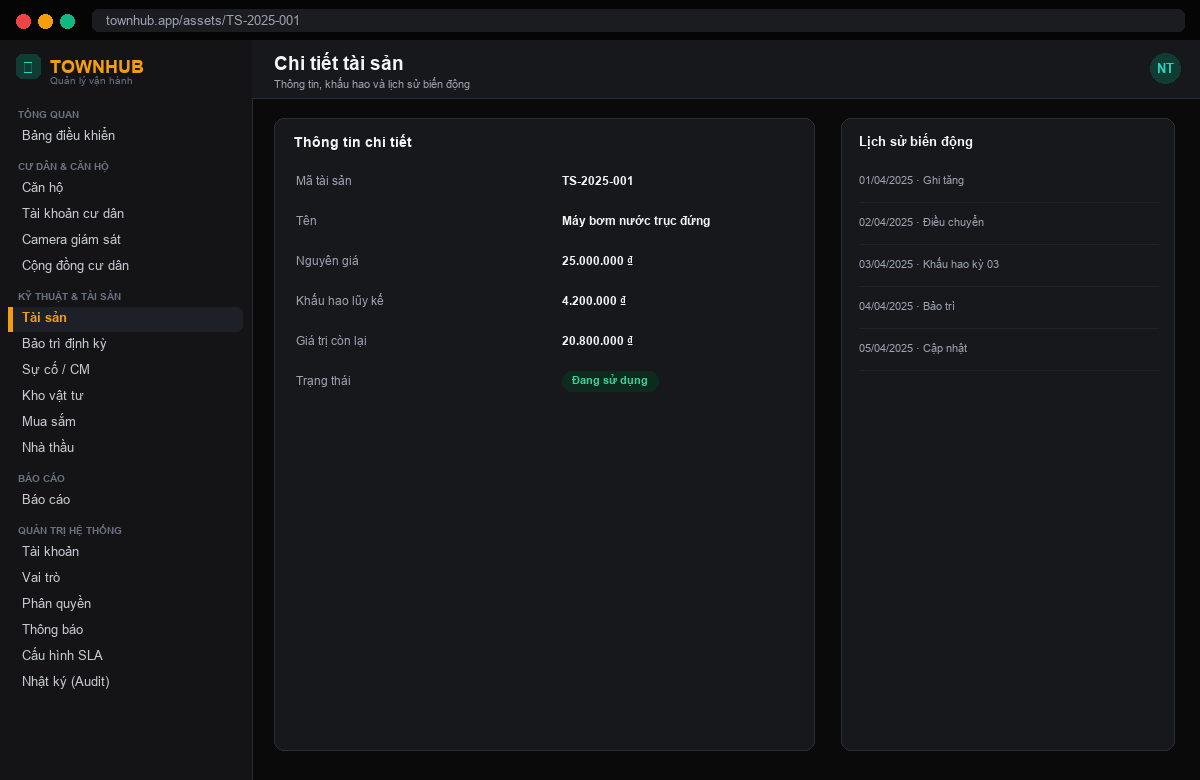
\includegraphics[width=\linewidth,height=0.82\textheight,keepaspectratio]{images/img18.png}
\caption*{\small Hình 4.7. Giao diện Chi tiết tài sản (thông số, khấu hao, lịch sử)}
\addcontentsline{lof}{figure}{Hình 4.7. Giao diện Chi tiết tài sản (thông số, khấu hao, lịch sử)}
\end{figure}
\begin{figure}[H]\centering
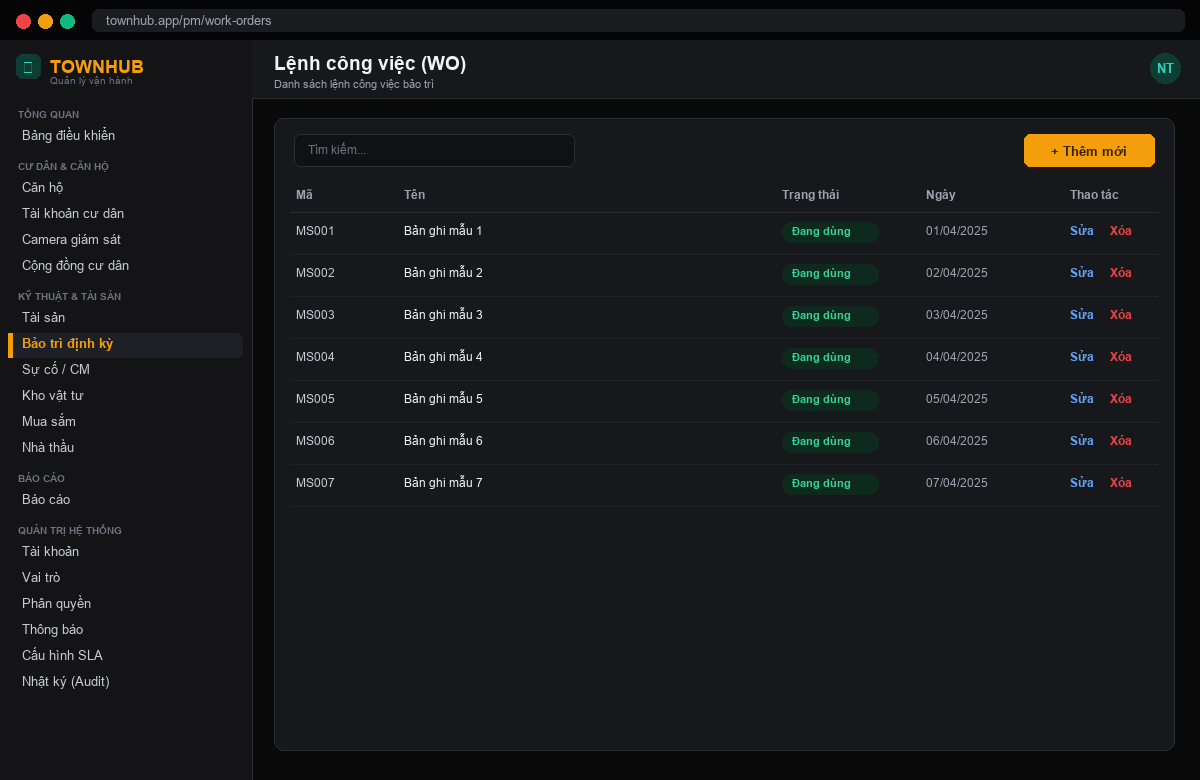
\includegraphics[width=\linewidth,height=0.82\textheight,keepaspectratio]{images/img19.png}
\caption*{\small Hình 4.8. Giao diện Lệnh công việc bảo trì (Work Order)}
\addcontentsline{lof}{figure}{Hình 4.8. Giao diện Lệnh công việc bảo trì (Work Order)}
\end{figure}
\phantomsection
\subsection*{4.1.7. Thành phần thông minh: sinh mã \& khấu hao tự động}
\addcontentsline{toc}{subsection}{4.1.7. Thành phần thông minh: sinh mã \& khấu hao tự động}
Đây là hai thành phần tự động hóa do tác giả tự thiết kế và cài đặt. Sinh mã tài sản tự động theo định dạng cấu hình (ví dụ \{DANH\_MUC\}-\{SO\_THU\_TU\}) với tiền tố lấy từ danh mục; kiểm tra trùng trước khi lưu. Khấu hao chạy tự động đầu tháng khi bật cờ tự động khấu hao, giảm thao tác thủ công của kế toán và bảo đảm khớp sổ kế toán.

\phantomsection
\section*{4.2. Nghiệp vụ Kho, Mua sắm và Nhà cung cấp}
\addcontentsline{toc}{section}{4.2. Nghiệp vụ Kho, Mua sắm và Nhà cung cấp}
\phantomsection
\subsection*{4.2.1. Đặt vấn đề và phạm vi}
\addcontentsline{toc}{subsection}{4.2.1. Đặt vấn đề và phạm vi}
Hoạt động bảo trì và xử lý sự cố cần vật tư; vật tư cần được quản lý tồn kho, bổ sung qua quy trình mua sắm và làm việc với nhà cung cấp. Phân hệ này quản lý ba mảng liên thông: Kho vật tư (tồn kho, xuất/nhập, kiểm kê), Mua sắm (đề xuất mua PR $\rightarrow$ đơn mua PO $\rightarrow$ hóa đơn) và Nhà cung cấp (hồ sơ, hợp đồng, đánh giá), kèm OCR hóa đơn để số hóa chứng từ.

\begin{itemize}[leftmargin=1.4em,itemsep=1pt,topsep=2pt]
  \item Quản lý kho, danh mục vật tư và mức tồn kho; cảnh báo tồn thấp.
  \item Xuất/nhập/điều chỉnh tồn qua phiếu giao dịch kho; kiểm kê.
  \item Quy trình mua sắm nhiều cấp: PR (đề xuất) $\rightarrow$ duyệt $\rightarrow$ PO (đơn mua) $\rightarrow$ Invoice (hóa đơn).
  \item Quản lý nhà cung cấp, hợp đồng (cảnh báo sắp hết hạn) và đánh giá hiệu suất.
  \item OCR hóa đơn tự động (VietOCR) để trích xuất dữ liệu hóa đơn.
\end{itemize}
\phantomsection
\subsection*{4.2.2. Mối liên hệ với Base và các phân hệ khác}
\addcontentsline{toc}{subsection}{4.2.2. Mối liên hệ với Base và các phân hệ khác}
Phân hệ do cá nhân em phát triển nhưng không hoạt động cô lập - dữ liệu và nghiệp vụ liên thông chặt chẽ với các phân hệ lân cận, đồng thời kế thừa các dịch vụ dùng chung do cả nhóm xây dựng:

\begin{itemize}[leftmargin=1.4em,itemsep=1pt,topsep=2pt]
  \item \textbf{Với Bảo trì \& Sự cố: }Work Order/ticket tiêu hao vật tư từ kho; khi thiếu vật tư có thể sinh đề xuất mua (PR).
  \item \textbf{Với Tài sản: }nhà cung cấp gắn với hợp đồng và tài sản (vendorId, vendorContractId); hóa đơn mua phục vụ ghi tăng tài sản.
  \item \textbf{Với Base: }phân quyền RBAC, thông báo cảnh báo tồn thấp/hợp đồng sắp hết hạn, tổng hợp chi phí lên Reporting.
\end{itemize}
\phantomsection
\subsection*{4.2.3. Phân tích yêu cầu chức năng}
\addcontentsline{toc}{subsection}{4.2.3. Phân tích yêu cầu chức năng}
\subsubsection*{a) Quản lý kho và vật tư}
Khai báo kho (Warehouse), danh mục vật tư (Material) và mức tồn (InventoryLevel). Mọi biến động tồn ghi qua InventoryTransaction (nhập/xuất/điều chỉnh). Hệ thống cảnh báo các vật tư dưới ngưỡng tồn tối thiểu (get-low-stock).

Quy trình kiểm kê kho định kỳ - chốt số liệu tồn hệ thống, đếm thực tế tại kho, đối chiếu chênh lệch và phê duyệt phiếu điều chỉnh - được minh họa ở Hình 4.9.

\begin{figure}[H]\centering

\includegraphics[width=\linewidth,height=0.82\textheight,keepaspectratio]{images/img20.pdf}
\caption*{\small Hình 4.9. Lưu đồ nghiệp vụ: Kiểm kê kho định kỳ}
\addcontentsline{lof}{figure}{Hình 4.9. Lưu đồ nghiệp vụ: Kiểm kê kho định kỳ}
\end{figure}
\subsubsection*{b) Quy trình mua sắm (PR $\rightarrow$ PO $\rightarrow$ Invoice)}
Người dùng lập Đề xuất mua (PurchaseRequest) gồm nhiều dòng vật tư; quản lý duyệt hoặc từ chối. PR đã duyệt được chuyển thành Đơn mua (PurchaseOrder) gửi nhà cung cấp; khi nhận hàng/hóa đơn tạo Invoice để đối chiếu. Quy trình duyệt nhiều cấp được cấu hình qua PoApprovalWorkflow. Toàn bộ quy trình mua sắm và bước OCR hóa đơn được minh họa ở Hình 4.10.

\begin{figure}[H]\centering
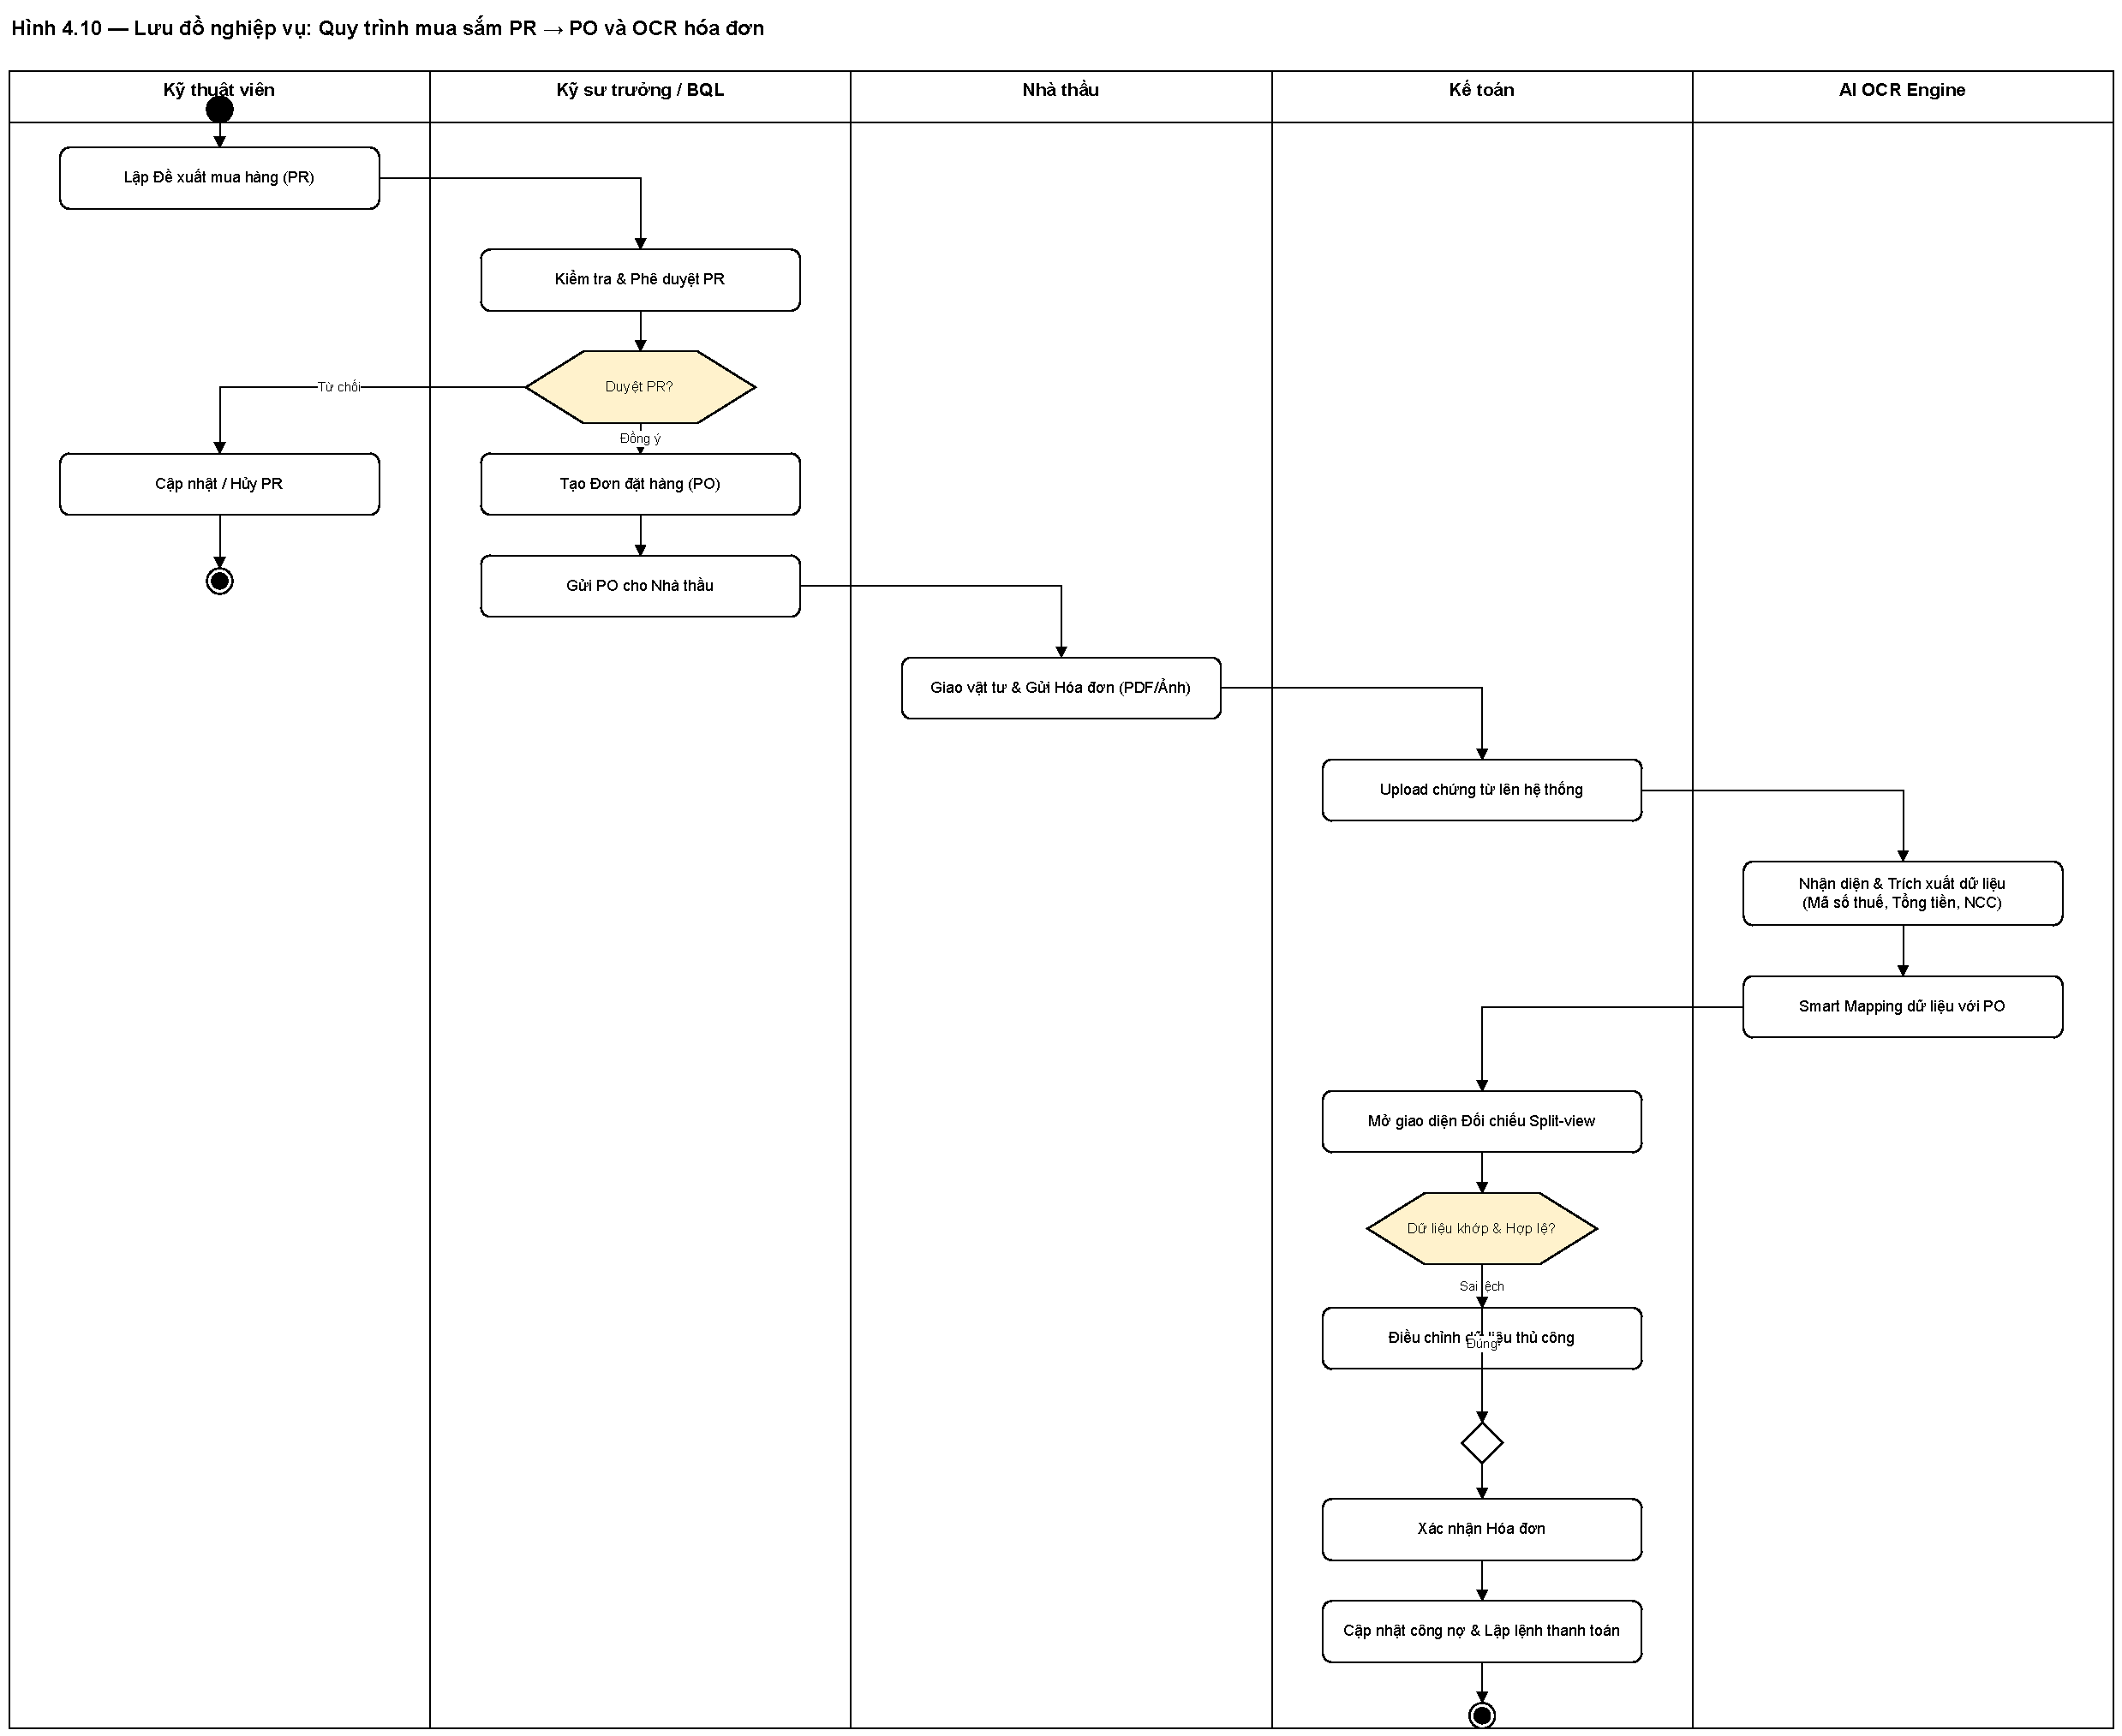
\includegraphics[width=\linewidth,height=0.82\textheight,keepaspectratio]{images/img21.pdf}
\caption*{\small Hình 4.10. Lưu đồ nghiệp vụ: Quy trình mua sắm PR $\rightarrow$ PO và OCR hóa đơn}
\addcontentsline{lof}{figure}{Hình 4.10. Lưu đồ nghiệp vụ: Quy trình mua sắm PR $\rightarrow$ PO và OCR hóa đơn}
\end{figure}
\subsubsection*{c) Quản lý nhà cung cấp}
Quản lý hồ sơ nhà cung cấp (Vendor) với thao tác blacklist/kích hoạt; hợp đồng (VendorContract) có cảnh báo sắp hết hạn (get-expiring) và các dịch vụ theo hợp đồng (VendorContractService); đánh giá hiệu suất định kỳ (VendorEvaluation).

\subsubsection*{d) OCR hóa đơn tự động}
Người dùng tải ảnh hóa đơn; hệ thống đẩy công việc vào hàng đợi OcrJobQueue; tiến trình nền OcrProcessingWorker gọi IInvoiceOcrEngine (bản cài đặt VietOcrEngine, có MockOcrEngine để kiểm thử) trích xuất các trường và tạo bản ghi Invoice để người dùng xác nhận. Xử lý nền giúp giao diện không bị chặn và mở rộng được số lượng công việc.

% ==== INJECTED: OCR use case + business flow + sequence (mục 4.2.5.d) ====
\medskip
\noindent\textbf{Đặc tả use case.} Nghiệp vụ OCR hóa đơn được đặc tả chi tiết ở bảng dưới đây. Đây là use case trung tâm của quy trình mua sắm: nó chuyển thao tác nhập liệu thủ công từng dòng hàng thành thao tác tải ảnh và xác nhận, đồng thời gắn kết quả trích xuất với Đơn mua (PO) để đối chiếu.

\begin{table}[H]
\centering
\caption*{\textbf{Bảng.} Đặc tả use case \emph{Trích xuất hóa đơn tự động (UC-OCR)}}
\label{tab:uc-ocr}
\renewcommand{\arraystretch}{1.3}
\small
\begin{tabularx}{\linewidth}{|>{\bfseries\raggedright\arraybackslash}p{0.22\linewidth}|X|}
\hline
Mã use case & UC-OCR — Trích xuất hóa đơn tự động \\ \hline
Tác nhân chính & Nhân viên kho / Nhân viên mua sắm (\emph{Người dùng}) \\ \hline
Tác nhân phụ & Dịch vụ OCR (FastAPI), tiến trình nền \texttt{OcrProcessingWorker} \\ \hline
Mục tiêu & Số hóa hóa đơn giấy/PDF thành các trường có cấu trúc (số hóa đơn, ngày, MST, tiền hàng, thuế, tổng) và bảng chi tiết hàng hóa, giảm nhập liệu thủ công và sai sót. \\ \hline
Tiền điều kiện & Người dùng đã đăng nhập, có quyền trên phân hệ Kho–Mua sắm; đã tồn tại PO cần đối chiếu (tùy chọn); dịch vụ OCR đang chạy. \\ \hline
Kích hoạt & Người dùng chọn chức năng \emph{Upload hóa đơn} và tải lên tệp ảnh/PDF. \\ \hline
Luồng chính &
1. Người dùng chọn engine OCR (mặc định \texttt{paddleocr}) và tải tệp hóa đơn lên.\newline
2. Backend .NET tạo bản ghi \texttt{ocr\_jobs} (trạng thái \emph{pending}) và đẩy vào hàng đợi \texttt{OcrJobQueue}, trả về ngay \texttt{jobId} (không chặn giao diện).\newline
3. \texttt{OcrProcessingWorker} lấy job khỏi hàng đợi, gọi \texttt{IInvoiceOcrEngine} $\rightarrow$ HTTP \texttt{POST /extract} sang dịch vụ OCR.\newline
4. Dịch vụ OCR tiền xử lý ảnh, chạy phát hiện + nhận dạng theo engine đã chọn, hậu xử lý (khử nghiêng, gom hàng, trích trường/bảng) và trả về JSON \{fields, lineItems, confidence\}.\newline
5. Worker chuẩn hóa kết quả, tạo bản ghi \texttt{Invoice}/\texttt{InvoiceItem} (trạng thái \emph{chờ xác nhận}) và cập nhật \texttt{ocr\_jobs} = \emph{done}.\newline
6. Người dùng mở màn hình xác nhận, đối chiếu với ảnh gốc và với PO, chỉnh sửa nếu cần rồi lưu chính thức. \\ \hline
Luồng thay thế / ngoại lệ &
3a. Tệp là PDF có lớp văn bản: hệ thống đọc thẳng text-layer, bỏ qua OCR ảnh.\newline
4a. Bố cục lạ hoặc chất lượng ảnh kém: người dùng chọn lại engine \texttt{vietocr} (độ chính xác nhận dạng cao nhất) hoặc bổ sung hóa đơn thật để fine-tune lại.\newline
4b. Dịch vụ OCR lỗi/timeout: job chuyển \emph{failed}, ghi log lỗi; người dùng có thể thử lại hoặc nhập tay.\newline
6a. Độ tin cậy (confidence) thấp hơn ngưỡng: hệ thống tô cảnh báo các trường nghi ngờ để người dùng kiểm tra kỹ. \\ \hline
Hậu điều kiện & Có bản ghi \texttt{Invoice} đã xác nhận, liên kết PO; số liệu sẵn sàng cho đối chiếu công nợ và báo cáo. \\ \hline
Yêu cầu phi chức năng & Xử lý bất đồng bộ (không chặn UI); truy vết trạng thái job; thay đổi engine không ảnh hưởng phần bóc tách trường. \\ \hline
\end{tabularx}
\end{table}

\noindent\textbf{Luồng xử lý theo thời gian.} Biểu đồ tuần tự dưới đây mô tả luồng của use case, làm rõ tính \emph{bất đồng bộ}: backend trả \texttt{jobId} cho người dùng ngay khi nhận tệp, còn việc gọi dịch vụ OCR và tạo \texttt{Invoice} diễn ra ở tiến trình nền; giao diện hỏi trạng thái theo chu kỳ (polling) cho tới khi job hoàn tất.

\begin{figure}[H]
\centering
\resizebox{\linewidth}{!}{%
\begin{tikzpicture}[font=\scriptsize\sffamily,>={Stealth[length=2mm]},
    msg/.style={->,thick},
    rmsg/.style={->,thick,dashed},
    lbl/.style={midway,above,font=\scriptsize,inner sep=1pt}]
  % --- lifelines (x coordinates fixed) ---
  \foreach \x/\name in {0/{Người dùng}, 2.8/{FE (Next.js)}, 5.6/{API (.NET)},
                        8.4/{Queue+Worker}, 11.2/{OCR svc}, 14/{CSDL}} {
     \node[draw,fill=blue!8,rounded corners,align=center,
           text width=1.9cm,minimum height=0.7cm] at (\x,0) {\name};
     \draw[dashed,gray] (\x,-0.6) -- (\x,-11.4);
  }
  % --- messages ---
  \draw[msg] (0,-1.3)   -- (2.8,-1.3)  node[lbl]{tải hóa đơn + chọn engine};
  \draw[msg] (2.8,-2.1) -- (5.6,-2.1)  node[lbl]{POST /invoices/ocr (file)};
  \draw[msg] (5.6,-2.9) -- (14,-2.9)   node[lbl]{tạo ocr\_jobs = pending};
  \draw[msg] (5.6,-3.7) -- (8.4,-3.7)  node[lbl]{enqueue(job)};
  \draw[rmsg] (5.6,-4.5) -- (2.8,-4.5) node[lbl]{trả jobId (202)};
  \draw[rmsg] (2.8,-5.1) -- (0,-5.1)   node[lbl]{hiển thị ``đang xử lý''};
  \draw[msg] (8.4,-6.1) -- (11.2,-6.1) node[lbl]{POST /extract (image, engine)};
  % self-processing activation on OCR lifeline
  \draw[fill=orange!15] (11.05,-6.5) rectangle (11.35,-7.5);
  \node[right,font=\scriptsize,text width=3cm] at (11.45,-7.0)
       {tiền xử lý $\rightarrow$ detect $\rightarrow$ recognize $\rightarrow$ parse};
  \draw[rmsg] (11.2,-7.9) -- (8.4,-7.9) node[lbl]{JSON \{fields, lineItems, conf\}};
  \draw[msg] (8.4,-8.7) -- (14,-8.7)   node[lbl]{lưu Invoice/InvoiceItem, job=done};
  \draw[msg] (0,-9.7) -- (5.6,-9.7)    node[lbl]{poll GET /ocr-jobs/\{id\}};
  \draw[rmsg] (5.6,-10.5) -- (0,-10.5) node[lbl]{done + dữ liệu để xác nhận};
\end{tikzpicture}}
\caption*{\small \textbf{Hình.} Biểu đồ tuần tự use case Trích xuất hóa đơn tự động (luồng bất đồng bộ hàng đợi–worker).}
\addcontentsline{lof}{figure}{Biểu đồ tuần tự use case Trích xuất hóa đơn tự động}
\label{fig:ocr-seq}
\end{figure}
% ==== END INJECTED ====


\phantomsection
\subsection*{4.2.4. Yêu cầu phi chức năng}
\addcontentsline{toc}{subsection}{4.2.4. Yêu cầu phi chức năng}
\begin{itemize}[leftmargin=1.4em,itemsep=1pt,topsep=2pt]
  \item Nhất quán tồn kho khi nhiều giao dịch đồng thời.
  \item Truy vết: mọi PR/PO/giao dịch kho đều lưu lịch sử và người thực hiện.
\end{itemize}
\phantomsection
\subsection*{4.2.5. Thiết kế phân hệ}
\addcontentsline{toc}{subsection}{4.2.5. Thiết kế phân hệ}
\subsubsection*{a) Danh sách Use Case chính}
Biểu đồ use case của phân hệ Kho – Mua sắm – Nhà cung cấp được thể hiện ở Hình 4.11.

\begin{figure}[H]\centering
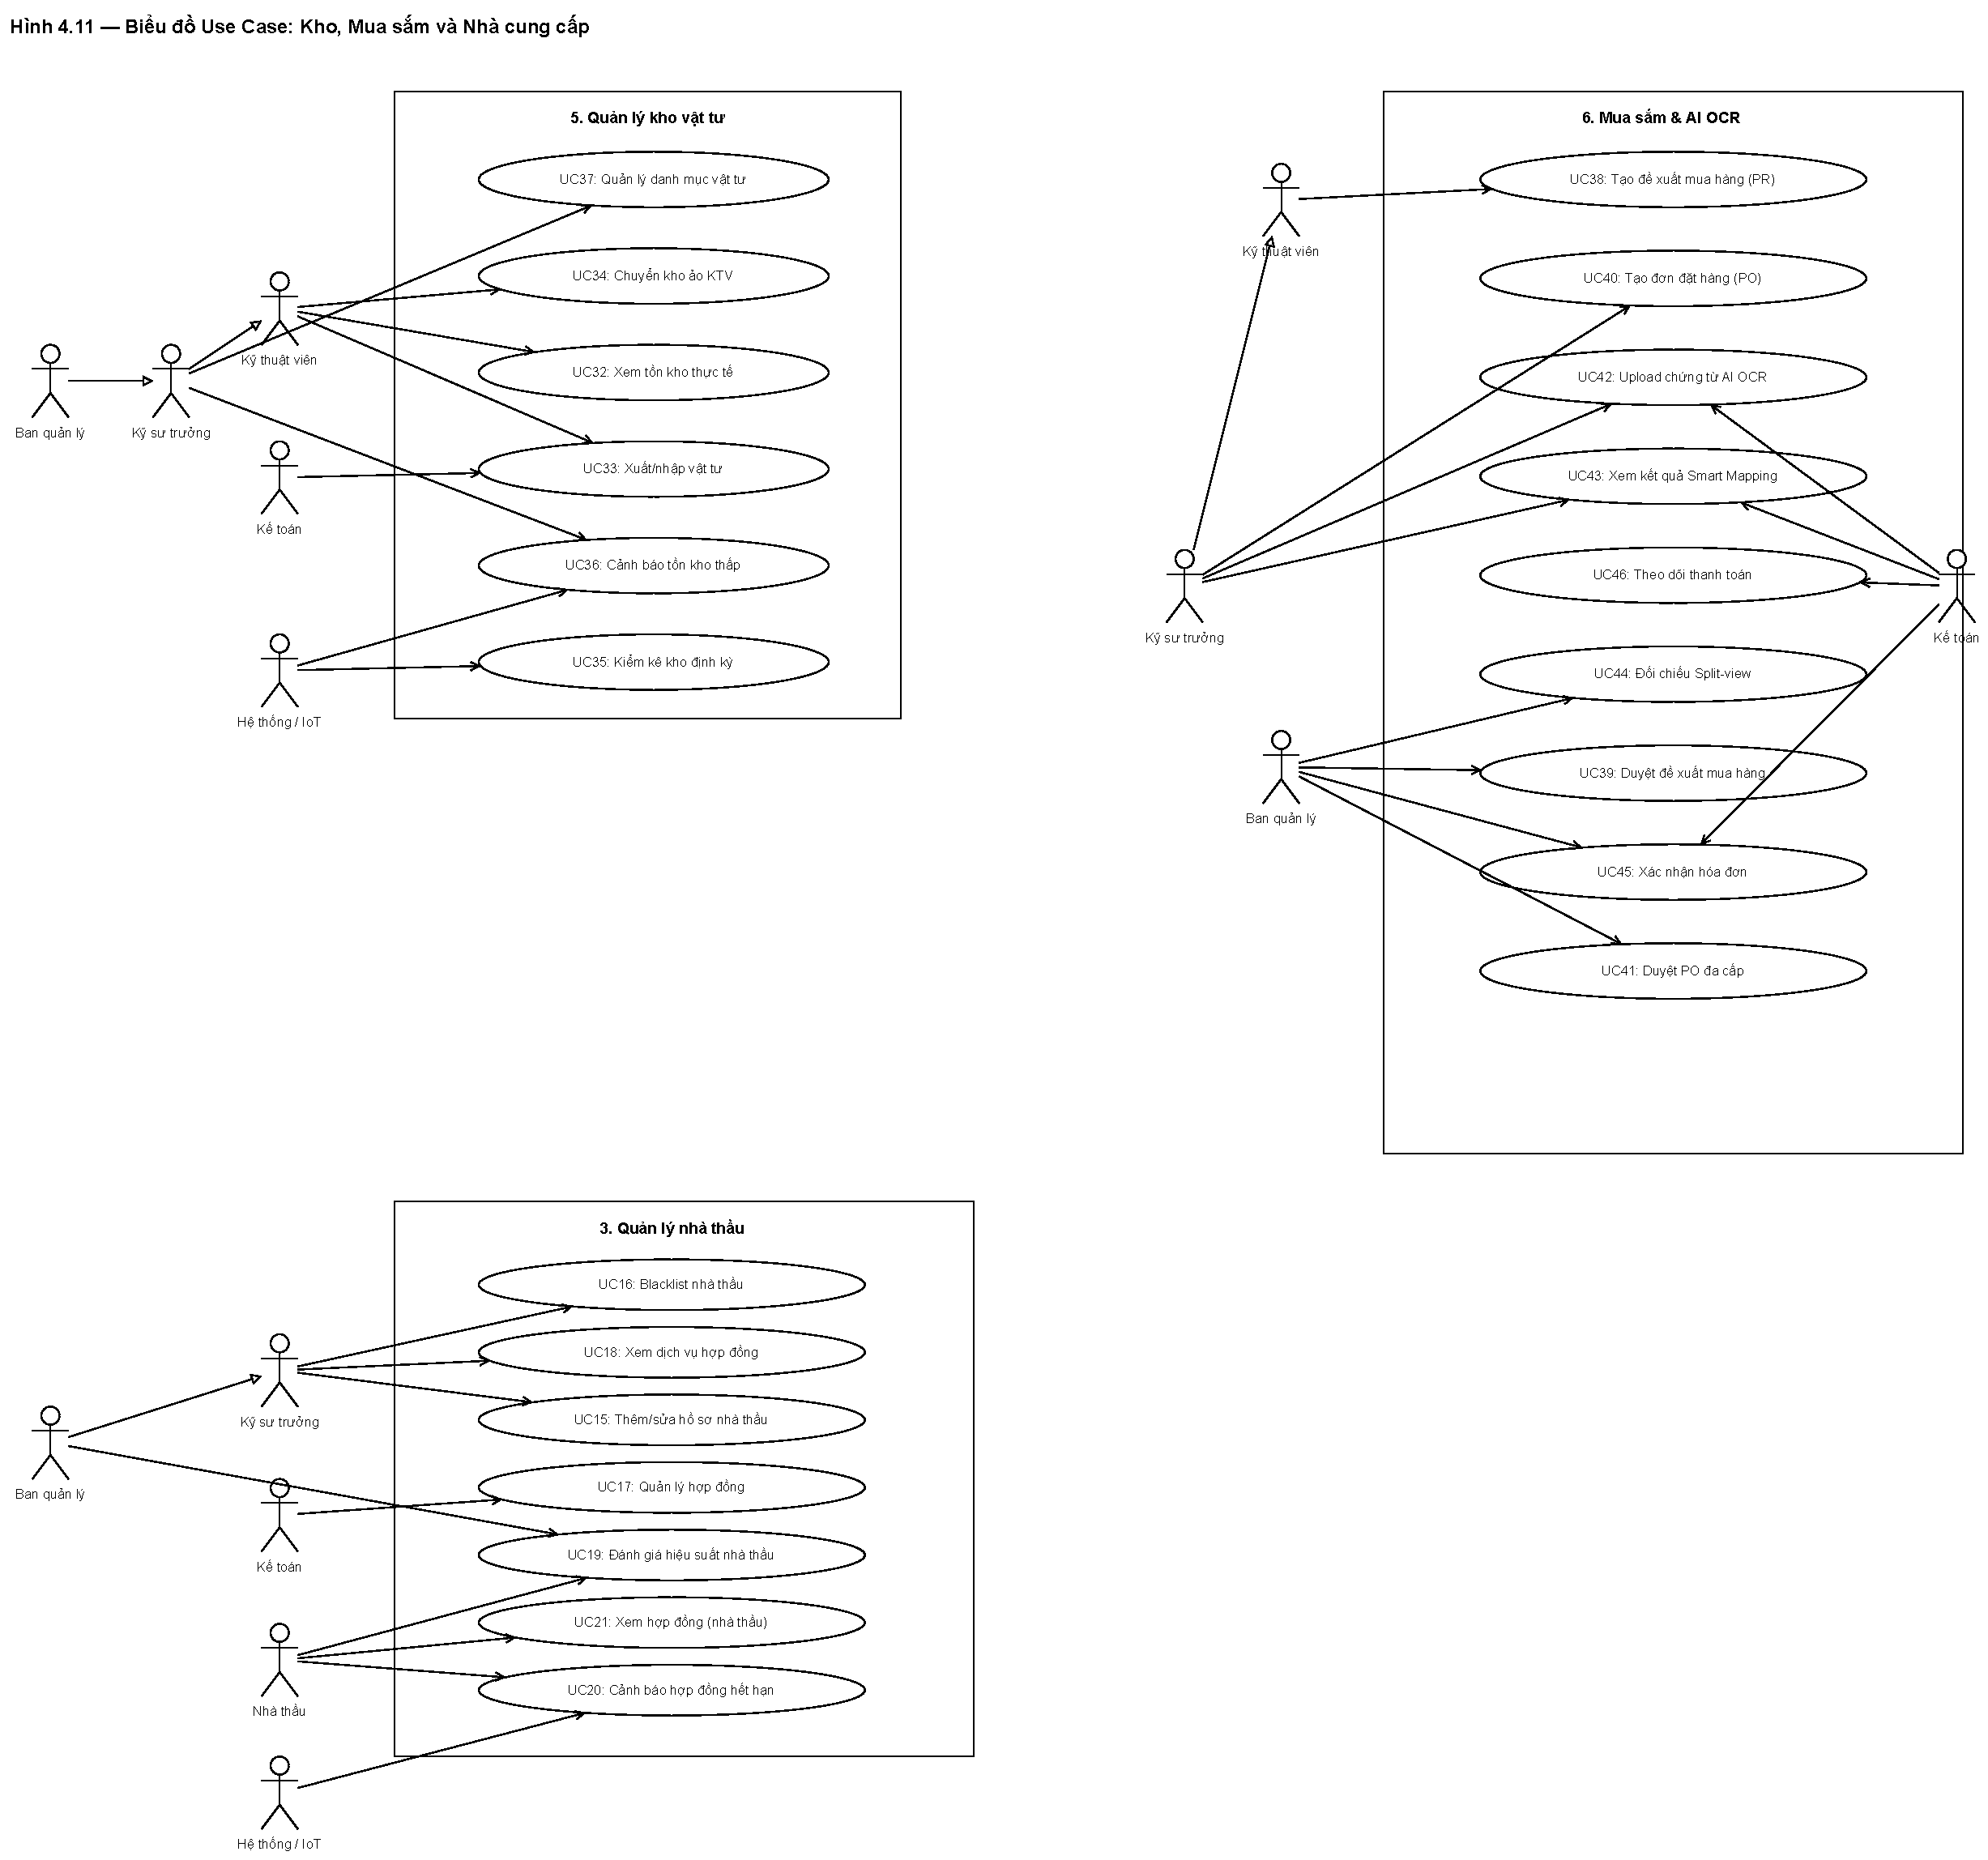
\includegraphics[width=\linewidth,height=0.82\textheight,keepaspectratio]{images/img22.pdf}
\caption*{\small Hình 4.11. Biểu đồ Use Case – Kho, Mua sắm và Nhà cung cấp}
\addcontentsline{lof}{figure}{Hình 4.11. Biểu đồ Use Case – Kho, Mua sắm và Nhà cung cấp}
\end{figure}
\begin{figure}[H]\centering
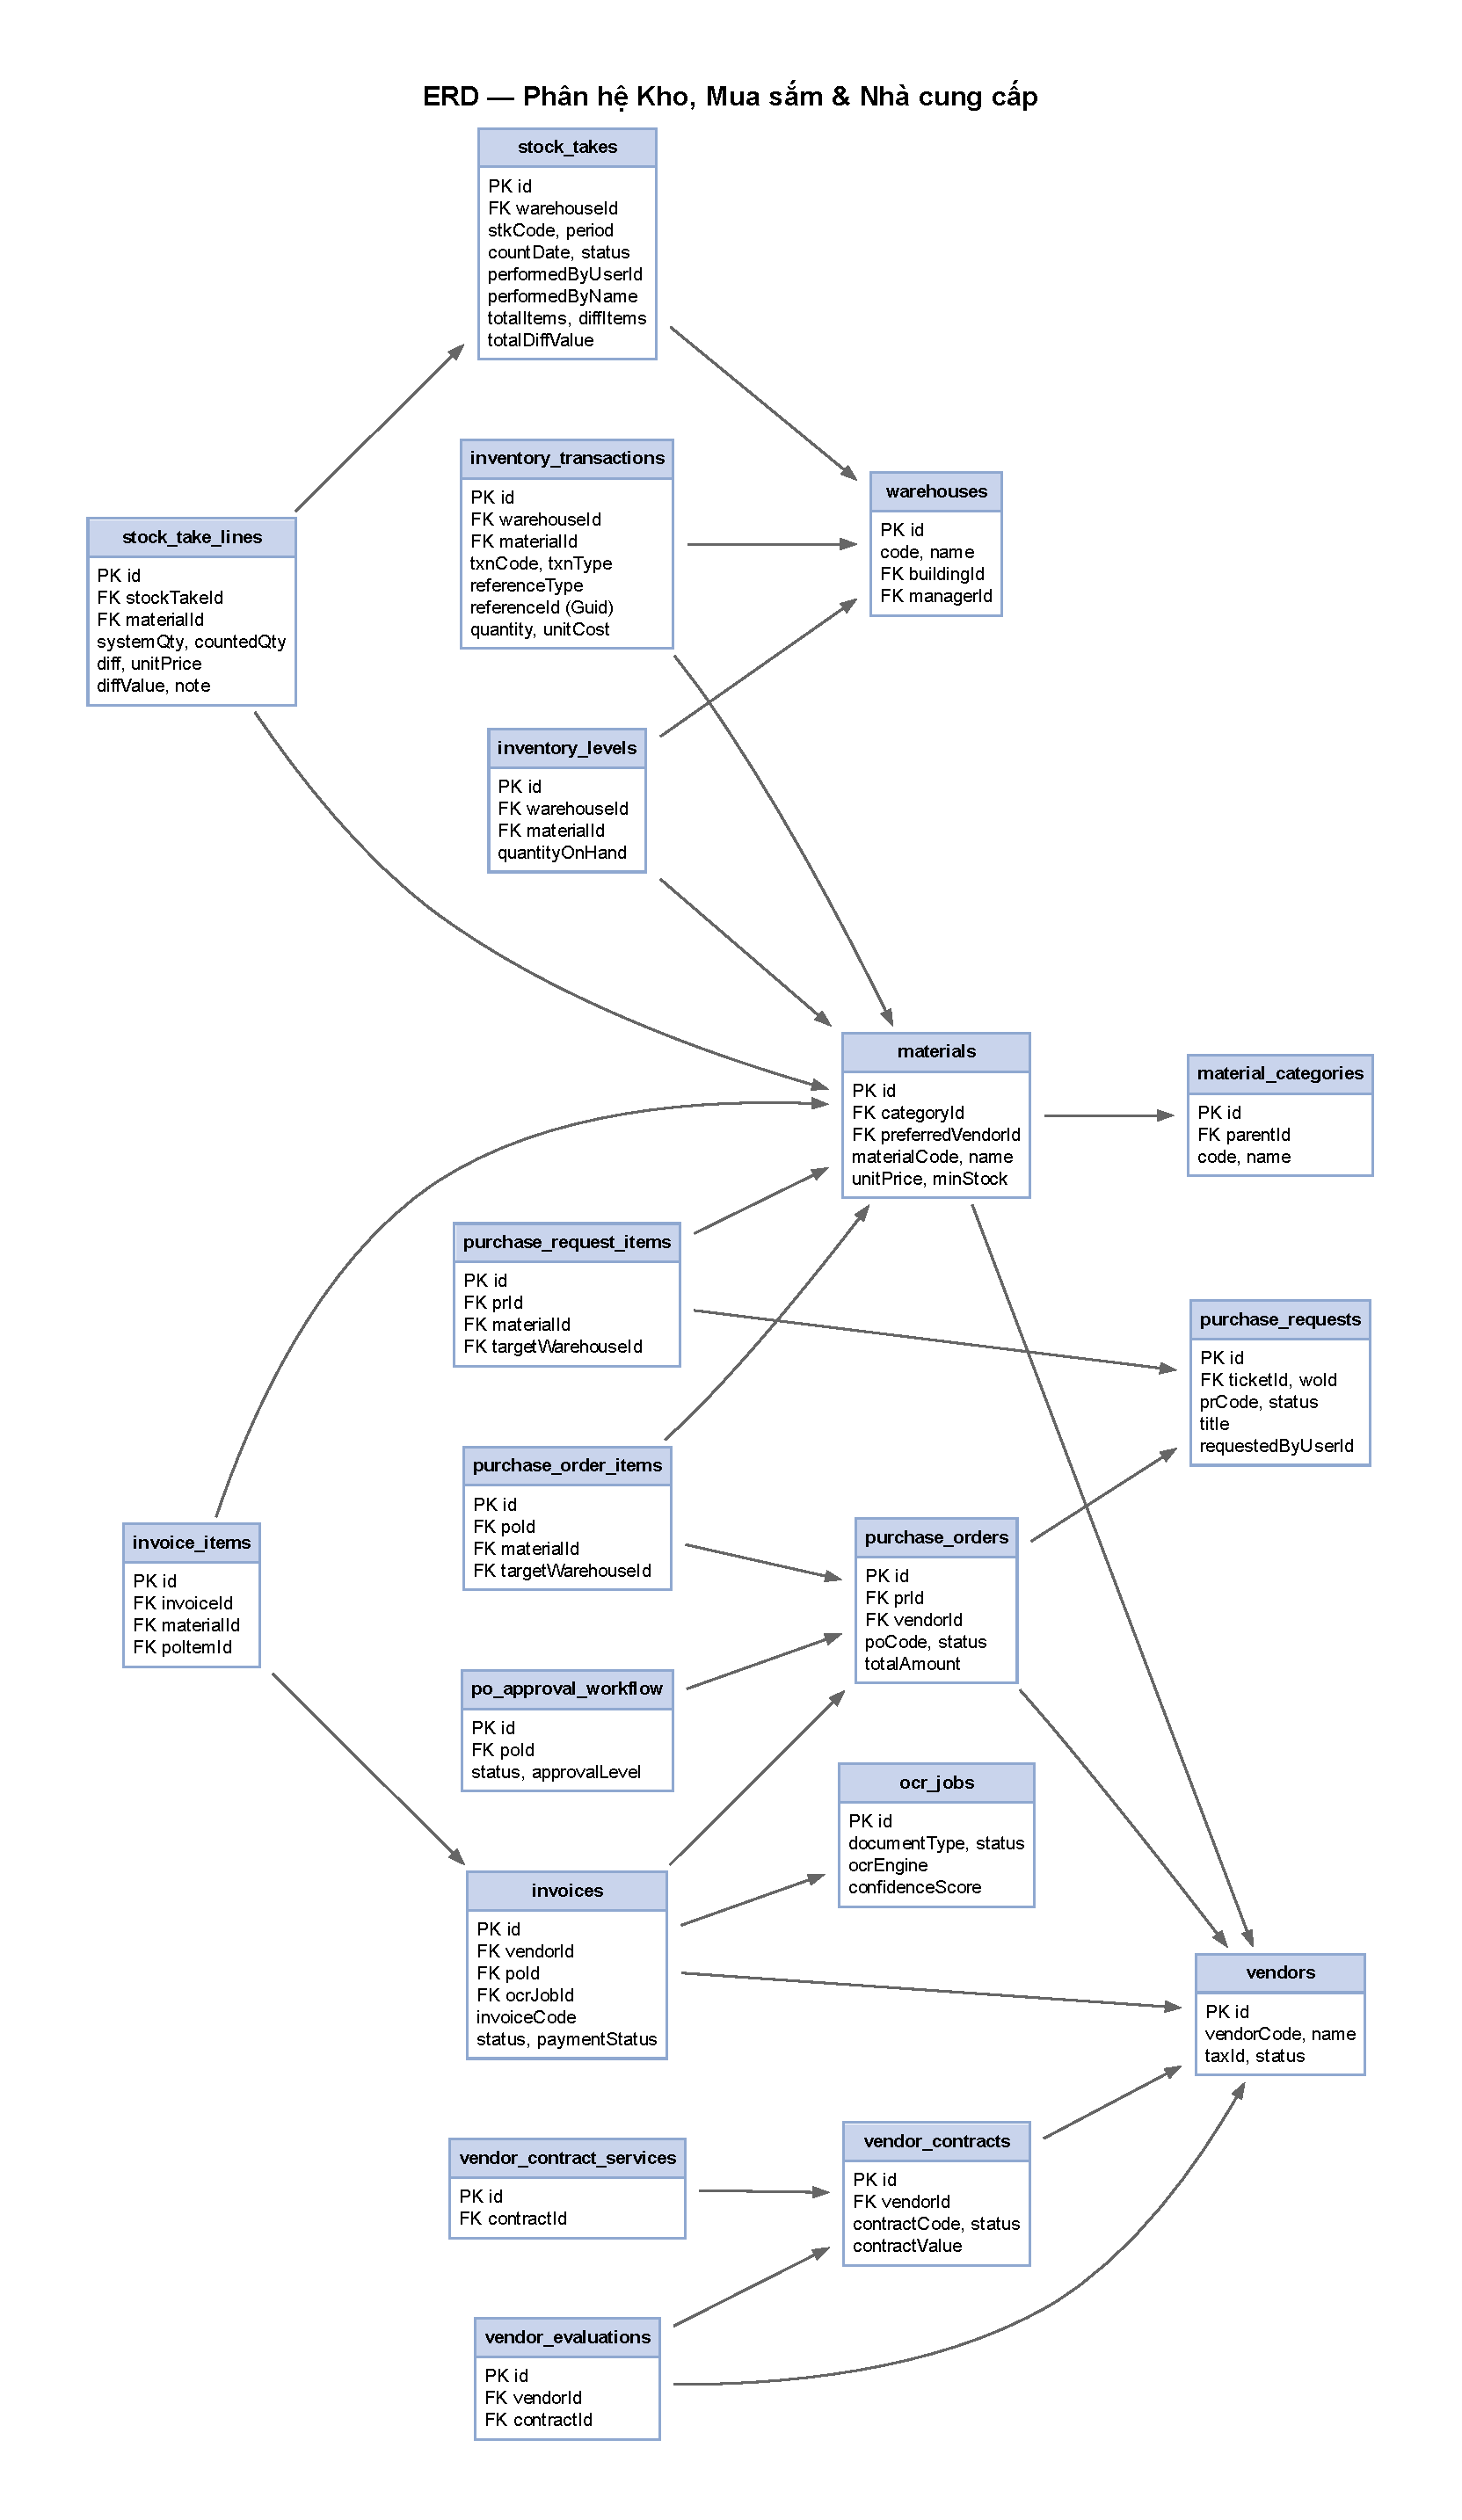
\includegraphics[width=\linewidth,height=0.9\textheight,keepaspectratio]{images/erd_kho.pdf}
\caption*{\small Hình 4.12. Sơ đồ thực thể – liên kết (ERD) phân hệ Kho, Mua sắm và Nhà cung cấp}
\addcontentsline{lof}{figure}{Hình 4.12. Sơ đồ thực thể – liên kết (ERD) phân hệ Kho, Mua sắm và Nhà cung cấp}
\end{figure}
\begin{center}{\singlespacing\renewcommand{\arraystretch}{1.25}
\begin{tabular}{|>{\raggedright\arraybackslash}p{\dimexpr\linewidth/3-2\tabcolsep-\arrayrulewidth\relax}|>{\raggedright\arraybackslash}p{\dimexpr\linewidth/3-2\tabcolsep-\arrayrulewidth\relax}|>{\raggedright\arraybackslash}p{\dimexpr\linewidth/3-2\tabcolsep-\arrayrulewidth\relax}|}
\hline
\textbf{Mã UC} & \textbf{Use case} & \textbf{Tác nhân} \\ \hline
UC-INV-01 & Quản lý kho \& vật tư, mức tồn & Thủ kho \\ \hline
UC-INV-02 & Nhập/​xuất/​kiểm kê vật tư & Thủ kho \\ \hline
UC-PR-01 & Lập \& duyệt/​từ chối đề xuất mua (PR) & NV mua sắm/​Quản lý \\ \hline
UC-PO-01 & Tạo đơn mua (PO) \& hóa đơn & NV mua sắm \\ \hline
UC-VD-01 & Quản lý nhà cung cấp \& hợp đồng & Quản lý \\ \hline
UC-VD-02 & Đánh giá hiệu suất nhà cung cấp & Quản lý \\ \hline
UC-OCR-01 & OCR hóa đơn tự động & NV mua sắm/​Hệ thống \\ \hline
\end{tabular}}\end{center}
\subsubsection*{b) Thiết kế cơ sở dữ liệu (thực thể chính)}
\begin{center}{\singlespacing\renewcommand{\arraystretch}{1.25}
\begin{tabular}{|>{\raggedright\arraybackslash}p{\dimexpr\linewidth/2-2\tabcolsep-\arrayrulewidth\relax}|>{\raggedright\arraybackslash}p{\dimexpr\linewidth/2-2\tabcolsep-\arrayrulewidth\relax}|}
\hline
\textbf{Thực thể} & \textbf{Ý nghĩa} \\ \hline
Warehouse, Material, InventoryLevel & Kho, danh mục vật tư, mức tồn \\ \hline
InventoryTransaction & Phiếu nhập/​xuất/điều chỉnh tồn \\ \hline
PurchaseRequest / PurchaseRequestItem & Đề xuất mua và dòng vật tư \\ \hline
PurchaseOrder / PurchaseOrderItem & Đơn mua và dòng hàng \\ \hline
Invoice / InvoiceItem, OcrJob & Hóa đơn, dòng hóa đơn, công việc OCR \\ \hline
Vendor, VendorContract, VendorContractService, VendorEvaluation & Nhà cung cấp, hợp đồng, dịch vụ, đánh giá \\ \hline
\end{tabular}}\end{center}
\subsubsection*{c) Thiết kế API}
\begin{center}{\singlespacing\renewcommand{\arraystretch}{1.25}
\begin{tabular}{|>{\raggedright\arraybackslash}p{\dimexpr\linewidth/2-2\tabcolsep-\arrayrulewidth\relax}|>{\raggedright\arraybackslash}p{\dimexpr\linewidth/2-2\tabcolsep-\arrayrulewidth\relax}|}
\hline
\textbf{Nhóm Endpoint} & \textbf{Chức năng} \\ \hline
/api/​asset/​warehouse/*, /api/​asset/​material/* & CRUD kho \& vật tư; get-low-stock, get-inventory-levels \\ \hline
/api/​asset/​inventory-transaction/* & Tạo \& tra cứu giao dịch kho \\ \hline
/api/​asset/​purchase-request/* & PR: tạo, duyệt (approve), từ chối (reject), thêm dòng \\ \hline
/api/​asset/​purchase-order/* & PO: tạo, cập nhật, thêm dòng \\ \hline
/api/​asset/​vendor/* & NCC: CRUD, blacklist, activate \\ \hline
/api/​asset/​vendor-contract/* & Hợp đồng: CRUD, get-expiring \\ \hline
/api/​asset/​vendor-evaluation/* & Đánh giá theo nhà cung cấp/​hợp đồng \\ \hline
\end{tabular}}\end{center}
\phantomsection
\subsection*{4.2.6. Thiết kế giao diện}
\addcontentsline{toc}{subsection}{4.2.6. Thiết kế giao diện}
\begin{center}{\singlespacing\renewcommand{\arraystretch}{1.25}
\begin{tabular}{|>{\raggedright\arraybackslash}p{\dimexpr\linewidth/2-2\tabcolsep-\arrayrulewidth\relax}|>{\raggedright\arraybackslash}p{\dimexpr\linewidth/2-2\tabcolsep-\arrayrulewidth\relax}|}
\hline
\textbf{Route} & \textbf{Chức năng} \\ \hline
/inventory, /inventory/​catalog & Tồn kho \& danh mục vật tư \\ \hline
/inventory/​stock-taking, /inventory/​transactions/​new & Kiểm kê \& tạo giao dịch \\ \hline
/procurement/​requests, /procurement/​orders, /procurement/​invoices & PR / PO / hóa đơn \\ \hline
/procurement/​ocr/​new, /procurement/​ocr/[id]/verify & OCR hóa đơn \& xác nhận \\ \hline
/vendors, /vendors/​contracts, /vendors/​performance & Nhà cung cấp, hợp đồng, hiệu suất \\ \hline
\end{tabular}}\end{center}
Một số màn hình tiêu biểu của phân hệ:

\begin{figure}[H]\centering
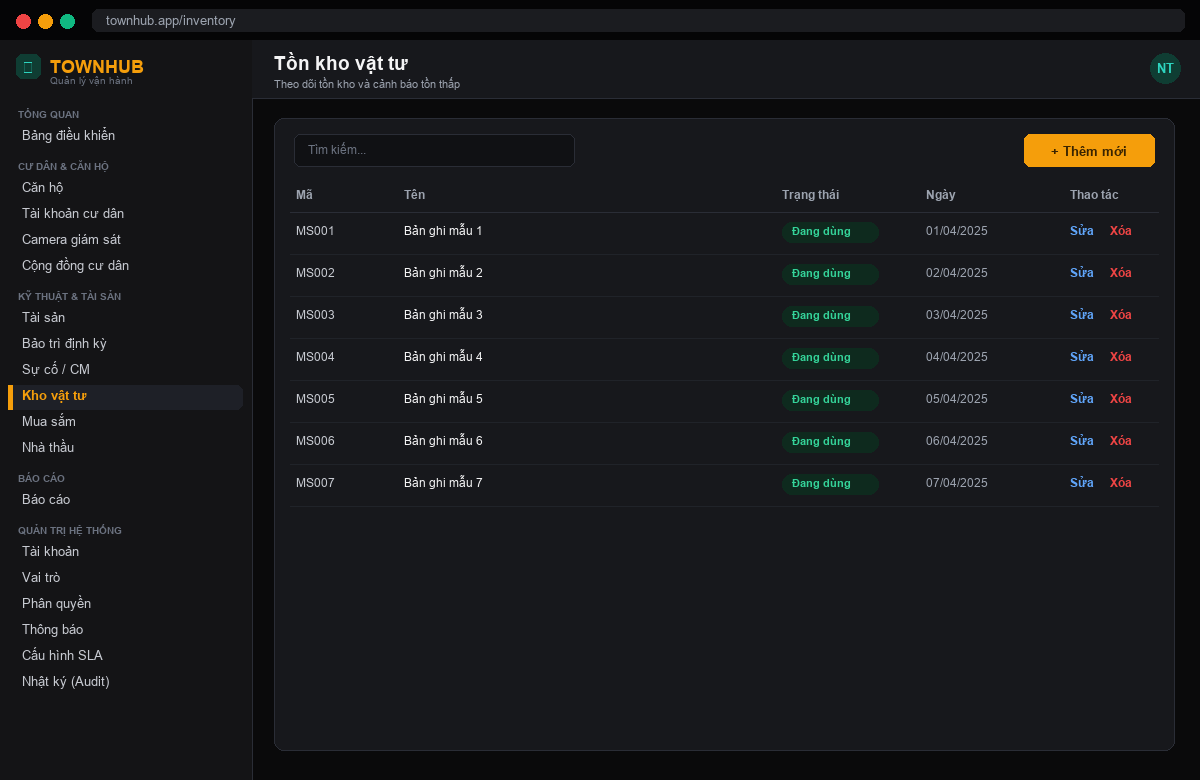
\includegraphics[width=\linewidth,height=0.82\textheight,keepaspectratio]{images/img24.png}
\caption*{\small Hình 4.13. Giao diện Tồn kho vật tư (cảnh báo tồn thấp)}
\addcontentsline{lof}{figure}{Hình 4.13. Giao diện Tồn kho vật tư (cảnh báo tồn thấp)}
\end{figure}
\begin{figure}[H]\centering
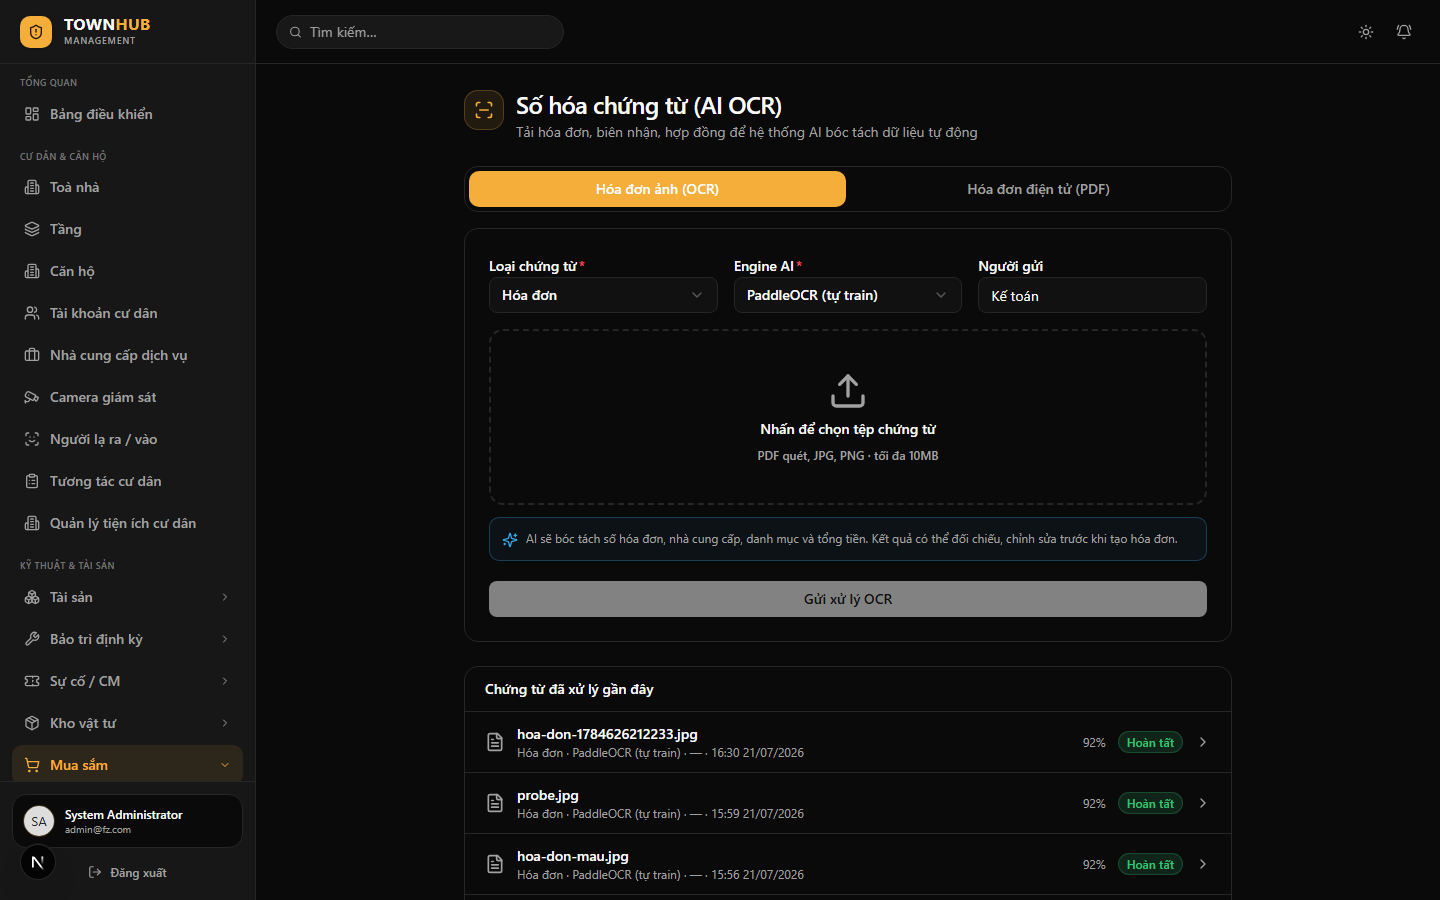
\includegraphics[width=\linewidth,height=0.82\textheight,keepaspectratio]{images/img25.png}
\caption*{\small Hình 4.14. Giao diện Upload OCR hóa đơn}
\addcontentsline{lof}{figure}{Hình 4.14. Giao diện Upload OCR hóa đơn}
\end{figure}
\begin{figure}[H]\centering
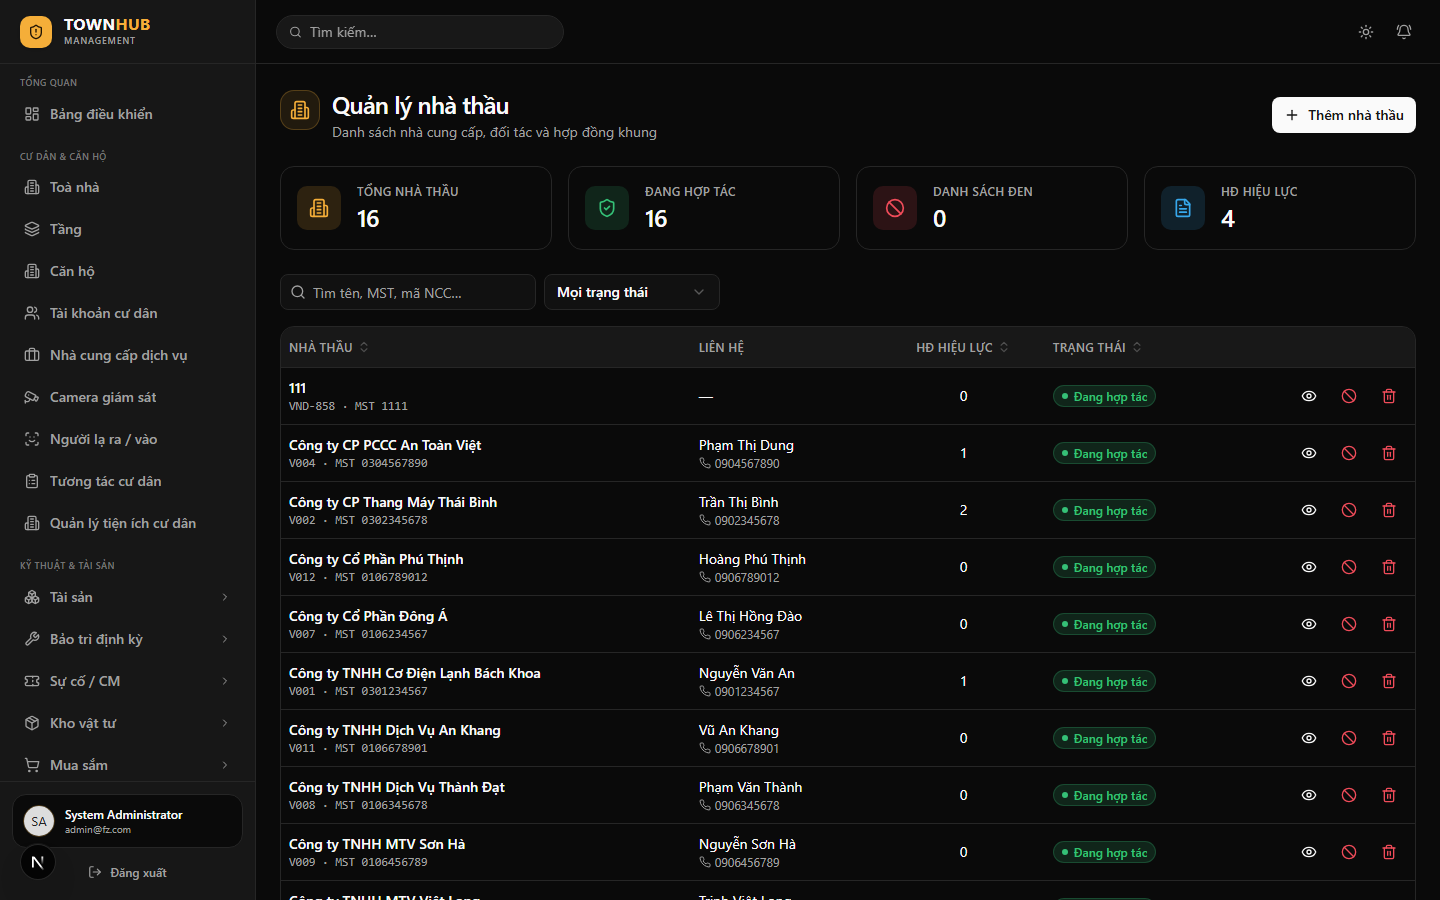
\includegraphics[width=\linewidth,height=0.82\textheight,keepaspectratio]{images/img26.png}
\caption*{\small Hình 4.15. Giao diện Danh sách nhà cung cấp}
\addcontentsline{lof}{figure}{Hình 4.15. Giao diện Danh sách nhà cung cấp}
\end{figure}
\phantomsection
\subsection*{4.2.7. Chi tiết kỹ thuật OCR hóa đơn: mô hình, huấn luyện và đánh giá}
\addcontentsline{toc}{subsection}{4.2.7. Chi tiết kỹ thuật OCR hóa đơn: mô hình, huấn luyện và đánh giá}
Mục này trình bày chi tiết thành phần AI/OCR dùng để số hóa hóa đơn trong phân hệ Kho – Mua sắm: kiến trúc dịch vụ, cơ sở lý thuyết các mô hình, quá trình huấn luyện trên dữ liệu tự sinh và kết quả đánh giá – so sánh giữa các engine. Đây là phần đóng góp kỹ thuật của tác giả cho phân hệ.

\subsubsection*{a) Kiến trúc dịch vụ OCR đa engine}
Dịch vụ OCR viết bằng Python/FastAPI, tách khỏi backend .NET và gọi qua HTTP POST /extract; chạy bất đồng bộ theo hàng đợi – tiến trình nền (OcrJobQueue $\rightarrow$ OcrProcessingWorker). Dịch vụ hỗ trợ ba chế độ chọn được trên giao diện (cột ocr\_jobs.ocrEngine), vừa để so sánh mô hình, vừa để chọn engine phù hợp từng loại chứng từ. Các engine OCR tự chủ đều quy kết quả về một cấu trúc dòng chuẩn hóa [\{text, box, prob\}] rồi dùng chung một hàm bóc tách trường (regex + luật vị trí), nên thay/đổi engine không ảnh hưởng phần lấy trường.

\begin{center}{\singlespacing\renewcommand{\arraystretch}{1.25}
\begin{tabular}{|>{\raggedright\arraybackslash}p{\dimexpr\linewidth/5-2\tabcolsep-\arrayrulewidth\relax}|>{\raggedright\arraybackslash}p{\dimexpr\linewidth/5-2\tabcolsep-\arrayrulewidth\relax}|>{\raggedright\arraybackslash}p{\dimexpr\linewidth/5-2\tabcolsep-\arrayrulewidth\relax}|>{\raggedright\arraybackslash}p{\dimexpr\linewidth/5-2\tabcolsep-\arrayrulewidth\relax}|>{\raggedright\arraybackslash}p{\dimexpr\linewidth/5-2\tabcolsep-\arrayrulewidth\relax}|}
\hline
\textbf{model} & \textbf{Phát hiện (detect)} & \textbf{Nhận dạng (recognize)} & \textbf{Fine-tune} & \textbf{Đặc điểm} \\ \hline
pdf & - (đọc lớp text) & pdfplumber & - & Hóa đơn điện tử có lớp text $\rightarrow$ đọc trực tiếp, chính xác nhất \\ \hline
vietocr & EasyOCR (CRAFT) & VietOCR (VGG + Transformer) & recognition & Tự chủ, mạnh về dấu tiếng Việt \\ \hline
paddleocr & PaddleOCR (DBNet) & PP-OCRv4 (SVTR\_LCNet) & detect + recognize & Hợp nhất, nhẹ, fine-tune cả hai tầng \\ \hline
paddledet\_viet & PaddleOCR (DBNet) & VietOCR (VGG + Transformer) & detect + recognition & Hybrid: DBNet mạnh + VietOCR đọc dấu tốt \\ \hline
\end{tabular}}\end{center}
\begin{figure}[H]\centering
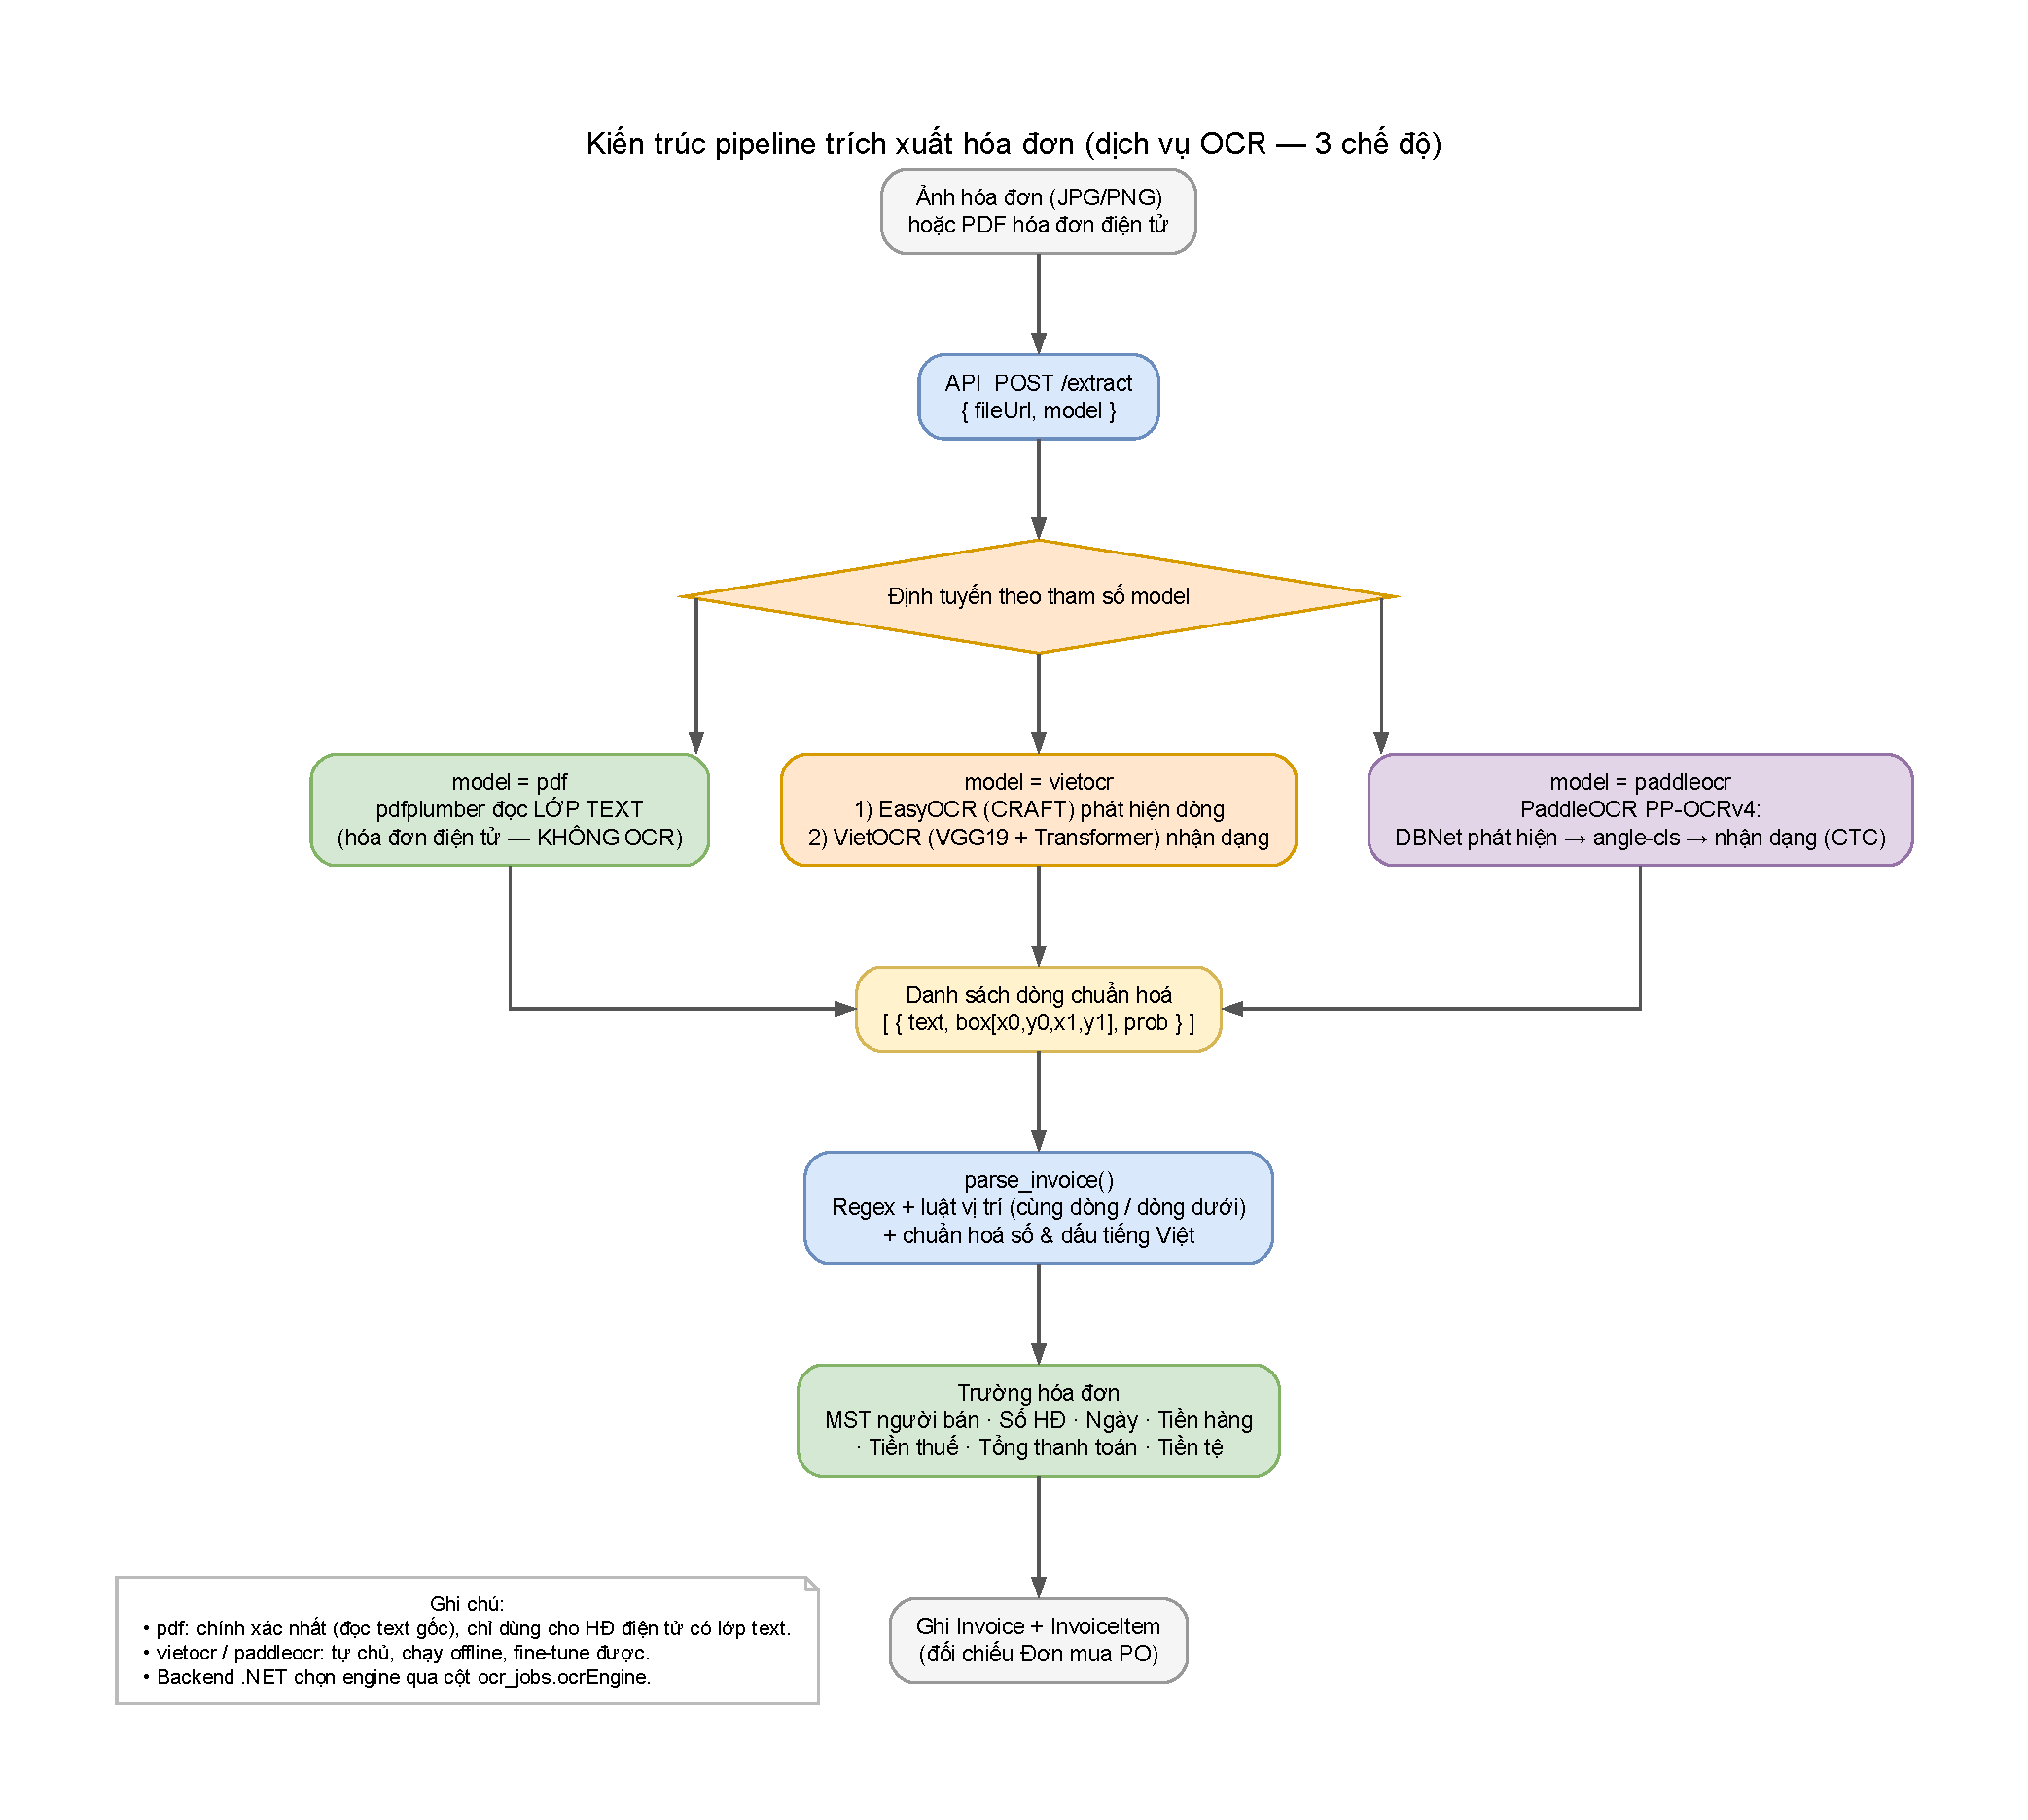
\includegraphics[width=\linewidth,height=0.82\textheight,keepaspectratio]{images/img27.pdf}
\caption*{\small Hình 4.16. Kiến trúc pipeline trích xuất hóa đơn (dịch vụ OCR ba chế độ)}
\addcontentsline{lof}{figure}{Hình 4.16. Kiến trúc pipeline trích xuất hóa đơn (dịch vụ OCR ba chế độ)}
\end{figure}
\subsubsection*{b) Cơ sở lý thuyết và thuật toán các mô hình}
\textbf{VietOCR (vgg\_transformer) - chỉ nhận dạng. }Gồm hai khối: (1) trích đặc trưng thị giác bằng CNN VGG19 (batch-norm) - nén chiều cao ảnh dòng về 1, giữ chiều rộng làm chuỗi đặc trưng; (2) Transformer encoder–decoder (seq2seq + attention) sinh lần lượt từng ký tự, huấn luyện bằng cross-entropy trên từ điển tiếng Việt (dịch vụ giải mã greedy). Ưu điểm: đọc dấu thanh rất tốt; nhược điểm: chỉ nhận dạng nên buộc ghép một bộ phát hiện bên ngoài.

\textbf{PaddleOCR (PP-OCRv4) - phát hiện + nhận dạng hợp nhất. }Ba bước: (1) DBNet (Differentiable Binarization) dự đoán bản đồ xác suất và bản đồ ngưỡng rồi nhị phân hóa khả vi ngay trong huấn luyện, tách biên vùng chữ gọn; (2) phân loại góc xoay dòng đúng chiều; (3) nhận dạng SVTR\_LCNet huấn luyện theo cơ chế GTC kết hợp CTC và NRTR (ghi nhận trong train.log qua CTCLoss/NRTRLoss), dùng bảng ký tự tiếng Việt dict\_vi.txt (137 ký tự). Ưu điểm: một bộ công cụ, det + rec đồng bộ, fine-tune được cả hai tầng, nhẹ, chạy offline.

\textbf{EasyOCR (CRAFT). }Pipeline vietocr chỉ mượn bộ phát hiện CRAFT của EasyOCR để cắt dòng (nhận dạng giao cho VietOCR). Vì CRAFT không được fine-tune trên dữ liệu hóa đơn nên trở thành nút cổ chai của pipeline này – đây cũng là lý do đề tài thử nghiệm biến thể hybrid \texttt{paddledet\_viet} (DBNet đã fine-tune + VietOCR) ở mục h.

% ==== INJECTED: model deep-dive (mục 4.2.7.b) ====
\medskip
\noindent\textbf{Chi tiết kiến trúc và công thức các mô hình.} Phần dưới đi sâu vào cơ chế toán học của từng thành phần để làm rõ vì sao mỗi mô hình phù hợp với một khâu của bài toán đọc hóa đơn (phát hiện vùng chữ, nhận dạng chuỗi, và huấn luyện đầu–cuối).

\noindent\textit{(1) VietOCR — trích đặc trưng VGG19 và bộ giải mã Transformer.}
Ảnh dòng chữ $I \in \mathbb{R}^{H\times W\times 3}$ được đưa qua CNN VGG19 (kèm batch-norm). Các tầng gộp (pooling) nén chiều cao về $1$ nhưng giữ chiều rộng, tạo chuỗi đặc trưng thị giác
\[
  X = (x_1, x_2, \dots, x_T), \qquad x_t \in \mathbb{R}^{d},
\]
với $T$ tỉ lệ theo bề rộng ảnh (mỗi $x_t$ ứng với một "lát" dọc của dòng chữ). Chuỗi này được bộ mã hóa Transformer tinh chỉnh bằng \emph{tự chú ý đa đầu} (multi-head self-attention):
\[
  \mathrm{Attention}(Q,K,V) = \mathrm{softmax}\!\left(\frac{QK^{\top}}{\sqrt{d_k}}\right)V,
\]
trong đó $Q,K,V$ là các phép chiếu tuyến tính của $X$ (kèm mã vị trí — positional encoding — để giữ thứ tự trái–phải của ký tự). Bộ giải mã sinh lần lượt từng ký tự $y_1,\dots,y_L$ theo cơ chế tự hồi quy, tối thiểu hóa hàm mất mát entropy chéo:
\[
  \mathcal{L}_{\text{seq2seq}} = -\sum_{t=1}^{L} \log P\!\left(y_t \mid y_{<t}, X\right).
\]
Khi suy luận, dịch vụ dùng giải mã tham lam (greedy): mỗi bước chọn $y_t=\arg\max_{y} P(y\mid y_{<t},X)$. Nhờ mô hình hóa phụ thuộc dài giữa các ký tự và có từ điển tiếng Việt riêng, VietOCR đọc dấu thanh (huyền, sắc, ngã, hỏi, nặng) rất chính xác; nhược điểm là mô hình \emph{chỉ nhận dạng}, buộc phải ghép một bộ phát hiện dòng bên ngoài.

\noindent\textit{(2) PaddleOCR (PP-OCRv4) — phát hiện DBNet, phân loại góc, nhận dạng SVTR\_LCNet.}
Tầng phát hiện dùng \emph{DBNet} với cơ chế nhị phân hóa khả vi (Differentiable Binarization). Thay cho phép nhị phân hóa cứng (không khả vi) trên bản đồ xác suất $P$, DBNet học đồng thời một bản đồ ngưỡng $T$ và xấp xỉ hàm bậc thang bằng một sigmoid dốc:
\[
  \hat{B}_{i,j} = \frac{1}{1 + e^{-k\,(P_{i,j} - T_{i,j})}},
\]
với $k$ là hệ số khuếch đại (thường $k=50$). Vì $\hat{B}$ khả vi nên biên vùng chữ được huấn luyện trực tiếp bằng lan truyền ngược; tổng mất mát gồm ba thành phần
\[
  \mathcal{L}_{\text{det}} = \mathcal{L}_{s} + \alpha\,\mathcal{L}_{b} + \beta\,\mathcal{L}_{t},
\]
lần lượt cho bản đồ xác suất, bản đồ nhị phân xấp xỉ và bản đồ ngưỡng. Sau phát hiện, một bộ phân loại góc (cls) xoay mỗi dòng về đúng chiều $0^{\circ}/180^{\circ}$. Tầng nhận dạng \emph{SVTR\_LCNet} kết hợp trộn đặc trưng cục bộ và toàn cục (local/global mixing) trên một xương sống nhẹ (LCNet), phù hợp chạy CPU. PP-OCRv4 huấn luyện recognizer theo cơ chế \emph{GTC} (Guided Training of CTC): nhánh chính dùng mất mát CTC
\[
  \mathcal{L}_{\text{CTC}} = -\log \!\!\sum_{\pi \in \mathcal{B}^{-1}(y)} \! P(\pi \mid X),
\]
trong đó $\mathcal{B}$ là toán tử gộp khung–bỏ ký tự trống (blank) ánh xạ đường căn chỉnh $\pi$ về chuỗi nhãn $y$; CTC cho phép huấn luyện không cần căn chỉnh ký tự–khung thủ công. Một nhánh chú ý phụ (NRTR) "dẫn dắt" nhánh CTC trong lúc huấn luyện (ghi nhận qua \texttt{CTCLoss}/\texttt{NRTRLoss} trong \texttt{train.log}) rồi được lược bỏ khi suy luận để giữ tốc độ. Ưu điểm nổi bật: một bộ công cụ hợp nhất, \emph{fine-tune được cả hai tầng} det+rec trên cùng dữ liệu tự gán nhãn, nhẹ và chạy offline.

\noindent\textit{(3) EasyOCR/CRAFT.}
Pipeline \texttt{vietocr} chỉ mượn bộ phát hiện \emph{CRAFT} của EasyOCR để định vị và cắt dòng (CRAFT dự đoán bản đồ vùng ký tự và bản đồ liên kết giữa các ký tự để gom thành từ/dòng), phần nhận dạng giao cho VietOCR. Vì CRAFT \emph{không được fine-tune} trên dữ liệu hóa đơn nên trở thành nút cổ chai của pipeline này — động lực dẫn tới biến thể hybrid \texttt{paddledet\_viet} ở mục h) (thay CRAFT bằng DBNet đã fine-tune, giữ recognizer VietOCR).

\noindent\textbf{So sánh vai trò.} Tổng hợp lại: DBNet/CRAFT giải bài toán \emph{định vị} (đâu là dòng chữ), còn VietOCR/SVTR\_LCNet giải bài toán \emph{đọc} (dòng chữ đó là gì); CTC và seq2seq là hai họ hàm mất mát khác nhau cho khâu đọc — CTC căn chỉnh ngầm và suy luận nhanh (một lượt), seq2seq+attention chính xác dấu thanh nhưng suy luận tuần tự nên chậm hơn. Chính sự khác biệt này dẫn tới các đánh đổi định lượng ở mục d) và lý do chọn engine ở mục e).
% ==== END INJECTED ====


\begin{figure}[H]\centering

\includegraphics[width=\linewidth,height=0.82\textheight,keepaspectratio]{images/img28.png}
\caption*{\small Hình 4.17. Luồng AI hai tầng (EasyOCR + VietOCR) so với PaddleOCR hợp nhất}
\addcontentsline{lof}{figure}{Hình 4.17. Luồng AI hai tầng (EasyOCR + VietOCR) so với PaddleOCR hợp nhất}
\end{figure}
\subsubsection*{c) Dữ liệu, huấn luyện và luồng xử lý}
Vì không có sẵn dữ liệu hóa đơn thật đã gán nhãn, đề tài tự sinh dữ liệu hóa đơn GTGT tiếng Việt tổng hợp (synthetic): script tự render hóa đơn và tự ghi lại tọa độ + nội dung từng ô chữ, nên xuất được cả nhãn phát hiện (det) lẫn nhận dạng (rec) mà không cần gán tay, kèm bảng ký tự dict\_vi.txt. Dữ liệu được random đa dạng bố cục và tăng cường cho ``giống thật'' (nền giấy, nghiêng/méo, nhiễu, nén JPEG, dấu mộc đỏ, chữ ký tay); mọi phép biến hình đều kéo theo tọa độ box nên nhãn luôn khớp. Quy mô mặc định 400–500 hóa đơn, chia train/val 90/10. Cả hai mô hình đều fine-tune từ trọng số pretrained (transfer learning) để hội tụ nhanh, cần ít dữ liệu. Cấu hình thật (đọc từ config.yml):

\begin{center}{\singlespacing\renewcommand{\arraystretch}{1.25}
\begin{tabular}{|>{\raggedright\arraybackslash}p{\dimexpr\linewidth/5-2\tabcolsep-\arrayrulewidth\relax}|>{\raggedright\arraybackslash}p{\dimexpr\linewidth/5-2\tabcolsep-\arrayrulewidth\relax}|>{\raggedright\arraybackslash}p{\dimexpr\linewidth/5-2\tabcolsep-\arrayrulewidth\relax}|>{\raggedright\arraybackslash}p{\dimexpr\linewidth/5-2\tabcolsep-\arrayrulewidth\relax}|>{\raggedright\arraybackslash}p{\dimexpr\linewidth/5-2\tabcolsep-\arrayrulewidth\relax}|}
\hline
\textbf{Mô hình} & \textbf{Thuật toán / Khởi tạo} & \textbf{Epoch} & \textbf{Batch} & \textbf{Optimizer / LR} \\ \hline
VietOCR (rec) & VGG19 + Transformer, từ vgg\_transformer & 20 000 iters & 32 & mặc định VietOCR \\ \hline
PaddleOCR rec & SVTR\_LCNet + GTC(CTC+NRTR), từ PP-OCRv4 & 80 & 64 & Adam + Cosine, lr 0,001 \\ \hline
PaddleOCR det & DBNet, từ PP-OCRv4 det & 150 & 8 & lr 0,001 \\ \hline
\end{tabular}}\end{center}
\textbf{Luồng xử lý. }Pipeline vietocr: ảnh $\rightarrow$ EasyOCR/CRAFT phát hiện dòng $\rightarrow$ cắt dòng $\rightarrow$ VietOCR (VGG19 $\rightarrow$ Transformer) $\rightarrow$ chuỗi text. Pipeline paddleocr: ảnh $\rightarrow$ DBNet phát hiện $\rightarrow$ phân loại góc $\rightarrow$ SVTR\_LCNet nhận dạng $\rightarrow$ chuỗi text. Cả hai gộp về danh sách dòng, đưa vào hàm bóc tách trường và ghi Invoice/InvoiceItem để đối chiếu PO.

\textbf{Kết quả huấn luyện PaddleOCR (số thật từ train.log). }Với nhận dạng (rec), loss giảm nhanh về gần 0 quanh bước \textasciitilde{}2 500 và độ chính xác huấn luyện tiến sát 1,0; trên tập val, accuracy toàn chuỗi đạt 0,9964 (99,64\%) và norm\_edit\_dis 0,9992 tại epoch 41. Với phát hiện (det), hmean tốt nhất trên val chỉ đạt 0,2298 (precision 0,228; recall 0,232) - cho thấy phát hiện bố cục hóa đơn học trên dữ liệu synthetic còn yếu; khuyến nghị bổ sung 50–150 hóa đơn thật gán bằng PPOCRLabel, hoặc kết hợp detector pretrain với recognizer đã fine-tune.

\begin{figure}[H]\centering
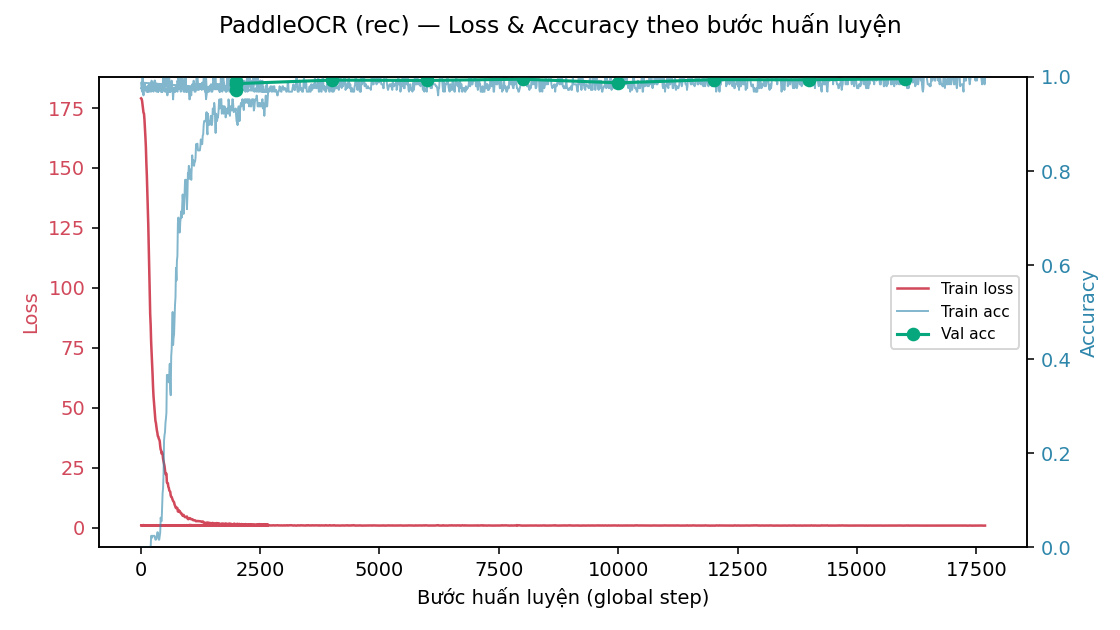
\includegraphics[width=\linewidth,height=0.82\textheight,keepaspectratio]{images/img29.png}
\caption*{\small Hình 4.18. Đường cong huấn luyện PaddleOCR (rec): loss và accuracy theo bước}
\addcontentsline{lof}{figure}{Hình 4.18. Đường cong huấn luyện PaddleOCR (rec): loss và accuracy theo bước}
\end{figure}
\subsubsection*{d) So sánh và đánh giá ba engine}
Ba engine (EasyOCR, VietOCR, PaddleOCR) được đánh giá trên cùng tập val 300 mẫu với các chỉ số: Seq-acc (đọc đúng toàn chuỗi), Char-acc (1 $-$ CER), NED, CER<0,1 và độ trễ (ms/ảnh, đo trên CPU):

\begin{landscape}\begin{center}{\footnotesize\singlespacing\renewcommand{\arraystretch}{1.25}
\begin{tabular}{|>{\raggedright\arraybackslash}p{\dimexpr\linewidth/6-2\tabcolsep-\arrayrulewidth\relax}|>{\raggedright\arraybackslash}p{\dimexpr\linewidth/6-2\tabcolsep-\arrayrulewidth\relax}|>{\raggedright\arraybackslash}p{\dimexpr\linewidth/6-2\tabcolsep-\arrayrulewidth\relax}|>{\raggedright\arraybackslash}p{\dimexpr\linewidth/6-2\tabcolsep-\arrayrulewidth\relax}|>{\raggedright\arraybackslash}p{\dimexpr\linewidth/6-2\tabcolsep-\arrayrulewidth\relax}|>{\raggedright\arraybackslash}p{\dimexpr\linewidth/6-2\tabcolsep-\arrayrulewidth\relax}|}
\hline
\textbf{Cấu hình} & \textbf{Seq-acc} & \textbf{Char-acc} & \textbf{NED} & \textbf{CER<0,1} & \textbf{ms/ảnh} \\ \hline
VietOCR gốc (trước) & 0,870 & 0,976 & 0,977 & 0,903 & - \\ \hline
VietOCR fine-tune (sau) & 1,000 & 1,000 & 1,000 & 1,000 & 317 \\ \hline
PaddleOCR gốc (trước) & 0,463 & 0,882 & 0,882 & 0,513 & - \\ \hline
PaddleOCR fine-tune (sau) & 0,893 & 0,967 & 0,968 & 0,913 & 65 \\ \hline
EasyOCR (baseline) & 0,510 & 0,811 & 0,818 & 0,613 & 156 \\ \hline
Ensemble (bỏ phiếu) & 0,920 & 0,974 & 0,974 & 0,933 & - \\ \hline
Oracle (best-of-3, chặn trên) & 1,000 & - & - & - & - \\ \hline
\end{tabular}}\end{center}\end{landscape}
\begin{figure}[H]\centering
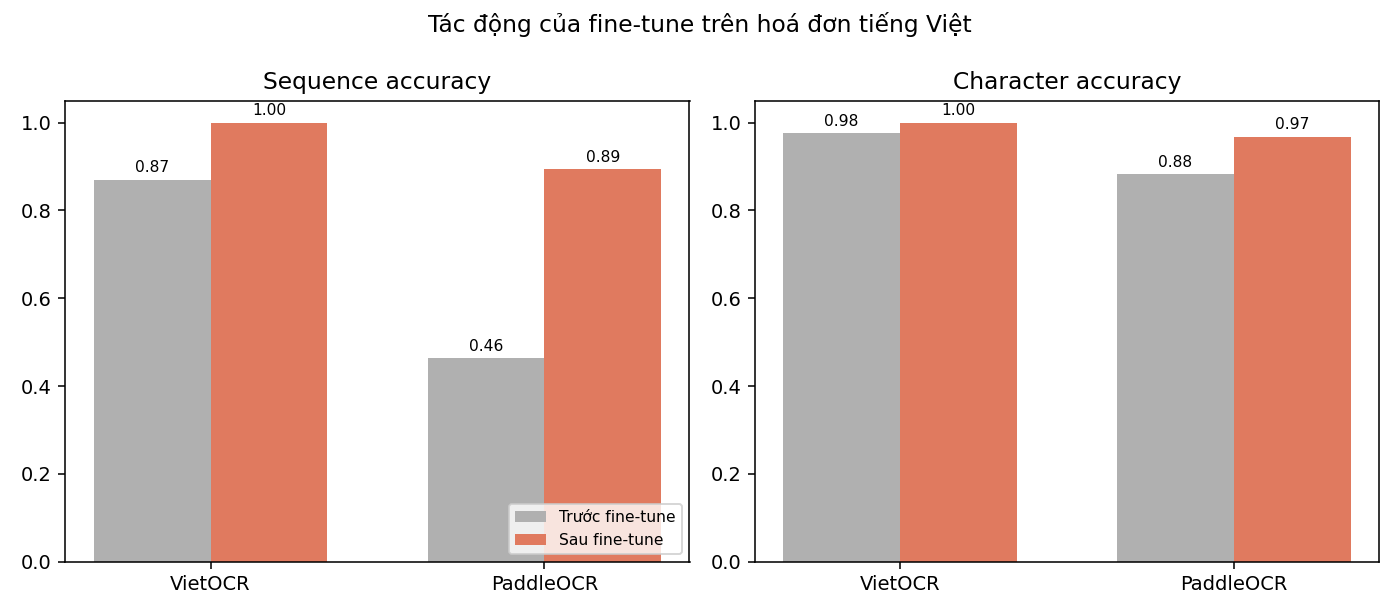
\includegraphics[width=\linewidth,height=0.82\textheight,keepaspectratio]{images/img30.png}
\caption*{\small Hình 4.19. Tác động của fine-tune (Sequence và Character accuracy)}
\addcontentsline{lof}{figure}{Hình 4.19. Tác động của fine-tune (Sequence và Character accuracy)}
\end{figure}
\begin{figure}[H]\centering
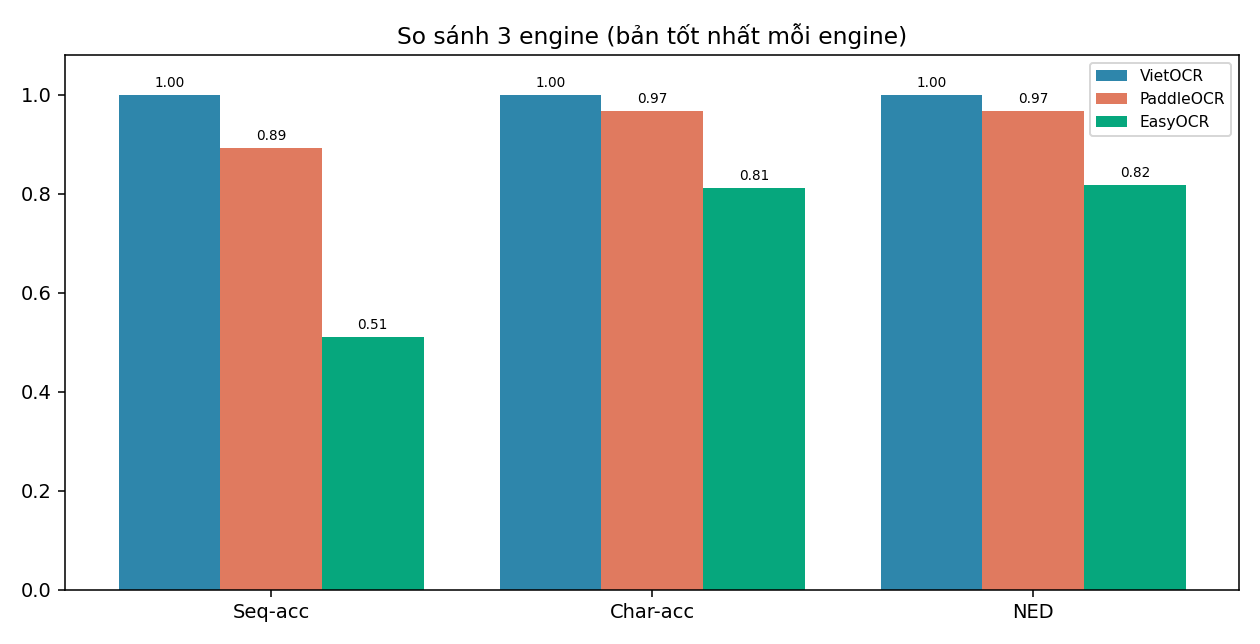
\includegraphics[width=\linewidth,height=0.82\textheight,keepaspectratio]{images/img31.png}
\caption*{\small Hình 4.20. So sánh ba engine theo Seq-acc / Char-acc / NED (tập val 300 mẫu)}
\addcontentsline{lof}{figure}{Hình 4.20. So sánh ba engine theo Seq-acc / Char-acc / NED (tập val 300 mẫu)}
\end{figure}
\textbf{Nhận xét. }(1) Fine-tune có tác động lớn: Seq-acc VietOCR tăng 0,870 $\rightarrow$ 1,000; PaddleOCR tăng 0,463 $\rightarrow$ 0,893 (PaddleOCR gốc pretrain tiếng Trung nên yếu trên tiếng Việt, hưởng lợi nhiều nhất). (2) Về độ chính xác nhận dạng, VietOCR fine-tune đứng đầu (đọc đúng cả 300/300 mẫu), trên PaddleOCR (0,893) và EasyOCR (0,510). (3) Về tốc độ, PaddleOCR nhanh nhất (65 ms/ảnh, nhanh hơn VietOCR \textasciitilde{}4,9 lần) và hợp nhất det+rec.

\begin{figure}[H]\centering
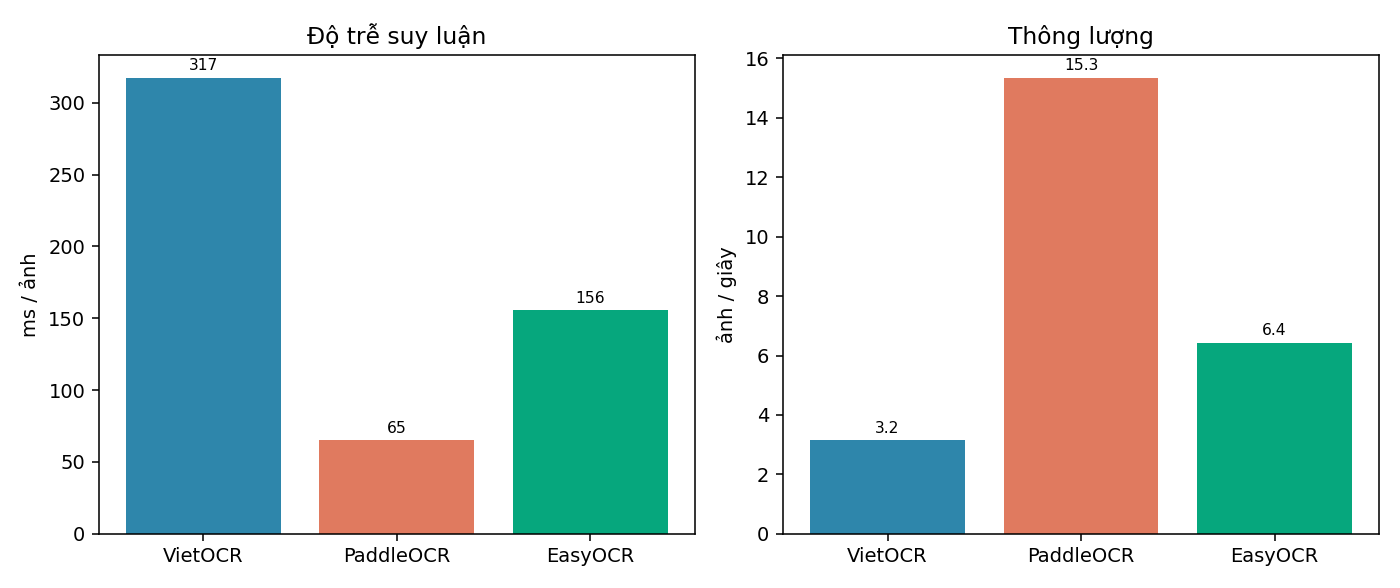
\includegraphics[width=\linewidth,height=0.82\textheight,keepaspectratio]{images/img32.png}
\caption*{\small Hình 4.21. Độ trễ suy luận (ms/ảnh) và thông lượng (ảnh/giây) trên CPU}
\addcontentsline{lof}{figure}{Hình 4.21. Độ trễ suy luận (ms/ảnh) và thông lượng (ảnh/giây) trên CPU}
\end{figure}
\begin{figure}[H]\centering
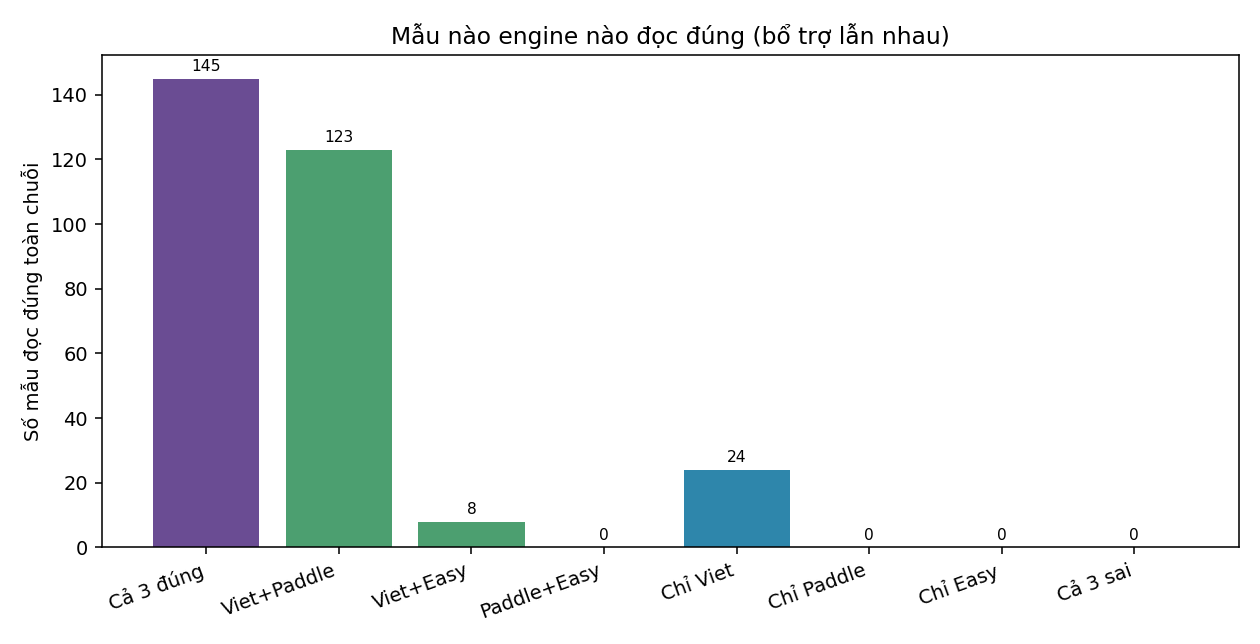
\includegraphics[width=\linewidth,height=0.82\textheight,keepaspectratio]{images/img33.png}
\caption*{\small Hình 4.22. Tính bổ trợ giữa các engine (mẫu nào engine nào đọc đúng)}
\addcontentsline{lof}{figure}{Hình 4.22. Tính bổ trợ giữa các engine (mẫu nào engine nào đọc đúng)}
\end{figure}
\textbf{Tính bổ trợ và kết hợp. }Trong 300 mẫu, số mẫu ``cả ba cùng sai'' = 0; VietOCR đọc đúng 300, PaddleOCR 268, EasyOCR 153; ``chỉ VietOCR đúng'' = 24, còn ``chỉ PaddleOCR/chỉ EasyOCR đúng'' = 0. Do đó bỏ phiếu ba engine chỉ đạt 0,920 - thấp hơn VietOCR đơn lẻ (1,000) vì bị kéo xuống bởi engine yếu hơn; cận trên Oracle = 1,000. Với bài toán này, dùng một engine mạnh hợp lý hơn là bỏ phiếu.

\subsubsection*{e) Lựa chọn mô hình}
\textbf{Vì sao chọn PaddleOCR thay vì kết hợp EasyOCR + VietOCR. }Phương án EasyOCR + VietOCR có recognizer VietOCR rất chính xác nhưng vướng ba nhược điểm: tầng phát hiện CRAFT của EasyOCR không được fine-tune (thành nút cổ chai), phải nạp hai bộ công cụ/hai mô hình (nặng), và chậm nhất (317 ms/ảnh). PaddleOCR là một bộ công cụ hợp nhất, fine-tune được cả DBNet lẫn recognizer trên cùng dataset tự gán nhãn, nhẹ và nhanh nhất (65 ms/ảnh). Vì vậy PaddleOCR được chọn làm engine tự chủ mặc định (đánh đổi một phần độ chính xác nhận dạng lấy pipeline gọn – nhanh – tinh chỉnh trọn gói); VietOCR được giữ làm lựa chọn khi cần độ chính xác nhận dạng cao nhất; biến thể hybrid \texttt{paddledet\_viet} kết hợp điểm mạnh hai bên; và chế độ PDF text-layer cho hóa đơn điện tử. Toàn bộ đều là giải pháp tự chủ, chạy offline, không phụ thuộc API bên ngoài.

\subsubsection*{f) Thuật toán bóc tách cấu trúc hóa đơn kháng nghiêng (deskew)}
\textbf{Đặt vấn đề. }Tầng OCR chỉ trả về danh sách ô văn bản kèm hộp bao (toạ độ), chưa phải dữ liệu có cấu trúc. Để dựng lại các trường (số hóa đơn, ngày, mã số thuế, các dòng tiền) và bảng chi tiết hàng hóa, hệ thống phải gom các ô về đúng hàng và cột dựa trên toạ độ. Ảnh hóa đơn chụp bằng điện thoại thường bị nghiêng vài độ; khi đó độ lệch tung độ giữa mép trái và mép phải của bảng (xấp xỉ tan$\theta$ nhân với bề rộng bảng) vượt quá chiều cao một dòng, khiến thao tác gom theo tung độ y gộp nhầm hai dòng sản phẩm liền kề vào cùng một hàng. Đề tài đề xuất thuật toán hai pha khắc phục bằng hình học – thống kê, chạy sau tầng OCR và không cần huấn luyện.

\textbf{Pha A – Ước lượng và khử nghiêng. }Các ô thuộc hàng tiêu đề bảng (STT, Tên hàng, ĐVT, SL, Đơn giá, Thành tiền) trong thực tế nằm trên cùng một phương ngang. Thuật toán lọc các ô này rồi khớp một đường thẳng qua tâm của chúng bằng phương pháp bình phương tối thiểu; hệ số góc a của đường thẳng chính là độ nghiêng của trang (góc $\theta$ = arctan a). Sau đó áp phép biến đổi trượt (shear) ngược trên trục tung cho mọi ô để nắn thẳng toạ độ:

\textit{a = $\Sigma$(xᵢ $-$ x̄)(yᵢ $-$ ȳ) / $\Sigma$(xᵢ $-$ x̄)²        ;        y$'$ = y $-$ a$\cdot$xᵢ}

Sau bước này, mọi ô thuộc cùng một dòng vật lý có tung độ y$'$ xấp xỉ bằng nhau (bảng được ``làm thẳng'' về mặt toạ độ mà không phải xử lý lại ảnh). Nếu |a| nhỏ hơn một ngưỡng $\varepsilon$ (ảnh vốn thẳng) thì bỏ qua bước trừ, bảo đảm tính bất biến với ảnh không nghiêng.

\textbf{Pha B – Tái tạo bảng theo cụm toạ độ. }Trên hệ toạ độ đã nắn thẳng, thuật toán lần lượt: (1) xác định biên bảng nằm giữa hàng tiêu đề và dòng ``Tổng/Thuế''; (2) gom dòng bằng phân cụm một chiều theo y$'$ với ngưỡng bằng 0,6 lần chiều cao dòng trung vị; (3) gán mỗi ô vào cột có tâm hoành độ gần nhất, riêng các cột số (SL, đơn giá, thành tiền) chọn ô gần tâm cột nhất thay vì nối chuỗi nhằm tránh dính các con số; (4) ghép mỗi cụm thành một dòng hàng và loại bỏ các dòng rác (không có mô tả chữ hoặc không có số tiền).

\begin{figure}[H]\centering
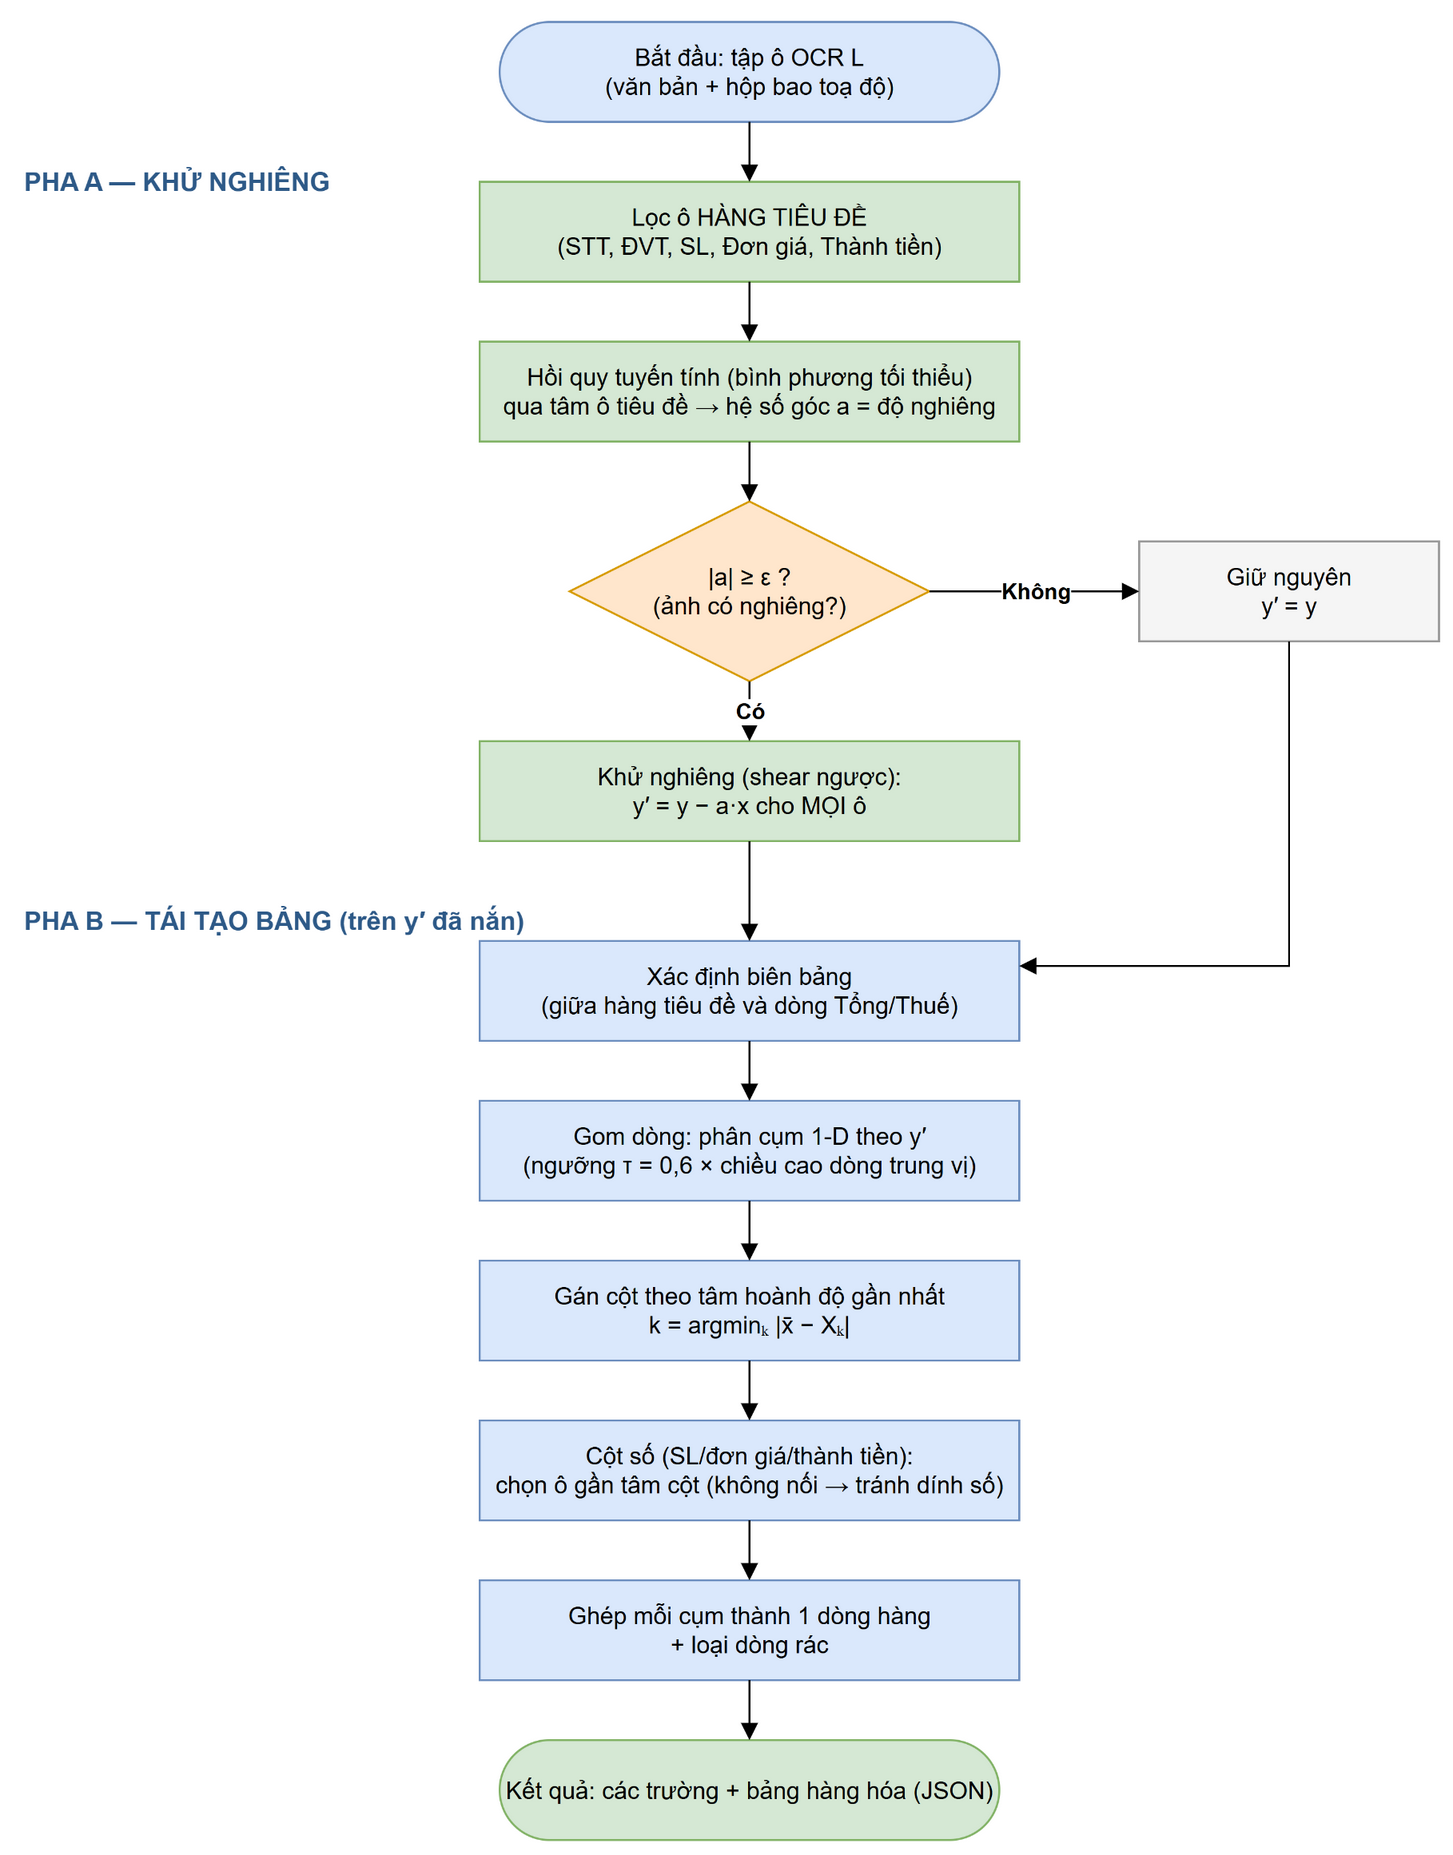
\includegraphics[width=\linewidth,height=0.82\textheight,keepaspectratio]{images/img34.png}
\caption*{\small Hình 4.23. Sơ đồ khối thuật toán bóc tách hóa đơn kháng nghiêng (deskew).}
\addcontentsline{lof}{figure}{Hình 4.23. Sơ đồ khối thuật toán bóc tách hóa đơn kháng nghiêng (deskew).}
\end{figure}
\textbf{Mã giả.} Toàn bộ thuật toán được tóm tắt như sau:

Thuật toán ExtractInvoiceTable(L)            \# L: tập ô OCR (văn bản + hộp bao)

  H   <- các ô có từ khóa cột tiêu đề

  a   <- HồiQuyHệSốGóc(\{ (xc, yc) : c thuộc H \})    \# bình phương tối thiểu

  nếu |a| >= eps:  y'(c) <- yc(c) - a * xc(c)   với mọi c thuộc L   \# khử nghiêng

  ngược lại:       y'(c) <- yc(c)

  Xk  <- tâm hoành độ các cột (từ H)

  tau <- 0.6 * trung\_vị(chiều cao ô)

  B   <- \{ c : y'\_tiêuđề < y'(c) < y'\_dừng \}        \# vùng bảng

  R   <- PhânCụm1D(B theo y', ngưỡng tau)           \# gom dòng

  với mỗi cụm r trong R:

      cột(c) <- argmin\_k |xc(c) - Xk|   với mọi c trong r

      dòng   <- \{ mô tả: nối ô chữ ; số: ô gần tâm mỗi cột số \}

      nếu hợp lệ: xuất dòng

  trả về R

\textbf{Độ phức tạp và kết quả.} Chi phí gồm hồi quy O(|H|), sắp xếp để gom cụm O(n log n) và gán cột O(n$\cdot$K) với K là số cột (khoảng 6), do đó tổng độ phức tạp là O(n log n) và bộ nhớ O(n), với n là số ô OCR. Trên hóa đơn thử nghiệm bị nghiêng, thuật toán tách đúng toàn bộ 7/7 dòng hàng cùng các trường tổng tiền, trong khi cách gom theo tung độ thô chỉ nhận được 3 hàng do bị dồn. Ưu điểm là thuần hình học – thống kê, không cần mạng nơ-ron, và tự bất biến khi ảnh đã thẳng.

\subsubsection*{g) Tổng hợp luồng xử lý AI end-to-end}
\textbf{Tổng quan. }Hình 4.24 tổng hợp toàn bộ luồng xử lý AI từ ảnh đầu vào đến JSON đầu ra, làm rõ dữ liệu đi qua những lớp nào, được xử lý và bóc tách ra sao, và vị trí của bước khử nghiêng.

\textbf{Các lớp xử lý. }(1) Đầu vào là ảnh hoặc tệp PDF hóa đơn. (2) Tiền xử lý (\_to\_images) chuyển PDF thành ảnh 200 dpi hoặc chuẩn hóa ảnh về hệ màu RGB. (3) Tùy engine người dùng chọn (trường ocrEngine truyền từ backend .NET), luồng rẽ nhánh giữa hai engine tự chủ: pipeline \texttt{vietocr} và pipeline \texttt{paddleocr}, cả hai đều đi tiếp qua lớp Phát hiện rồi Nhận dạng. (4) Lớp Phát hiện: pipeline vietocr dùng EasyOCR/CRAFT để tìm và cắt từng dòng, pipeline paddleocr dùng DBNet kèm bộ phân loại góc (cls). (5) Lớp Nhận dạng: VietOCR (VGG19 + Transformer) hoặc SVTR\_LCNet (PP-OCRv4, đã fine-tune) đọc chữ, tạo ra danh sách ô OCR gồm văn bản, hộp bao (toạ độ) và độ tin cậy.

\textbf{Bóc tách và vị trí khử nghiêng. }(6) Lớp Hậu xử lý (parse) biến danh sách ô rời rạc thành dữ liệu có cấu trúc qua năm bước: \textcircled{\scriptsize 1} Khử nghiêng (deskew) — ước lượng độ nghiêng từ hàng tiêu đề và nắn toạ độ theo y$'$ = y $-$ a$\cdot$x; \textcircled{\scriptsize 2} Gom hàng theo y$'$ đã nắn; \textcircled{\scriptsize 3} Trích các trường bằng nhãn và biểu thức chính quy (số hóa đơn, ngày, MST, tiền hàng, thuế, tổng); \textcircled{\scriptsize 4} Trích bảng chi tiết bằng cách gán ô vào cột theo tâm hoành độ; \textcircled{\scriptsize 5} Chuẩn hóa con số và bù giá trị tổng. Đáng chú ý, khử nghiêng là bước ĐẦU TIÊN của lớp hậu xử lý, chạy ngay sau khi có danh sách ô OCR và trước mọi thao tác gom hàng, gán cột — vì các bước sau đều dựa trên toạ độ đã được nắn thẳng. (7) Đầu ra là JSON gồm fields, lineItems và confidence, được backend .NET lưu vào Invoice/InvoiceItem và hiển thị ở màn hình xác nhận.

\begin{figure}[H]\centering
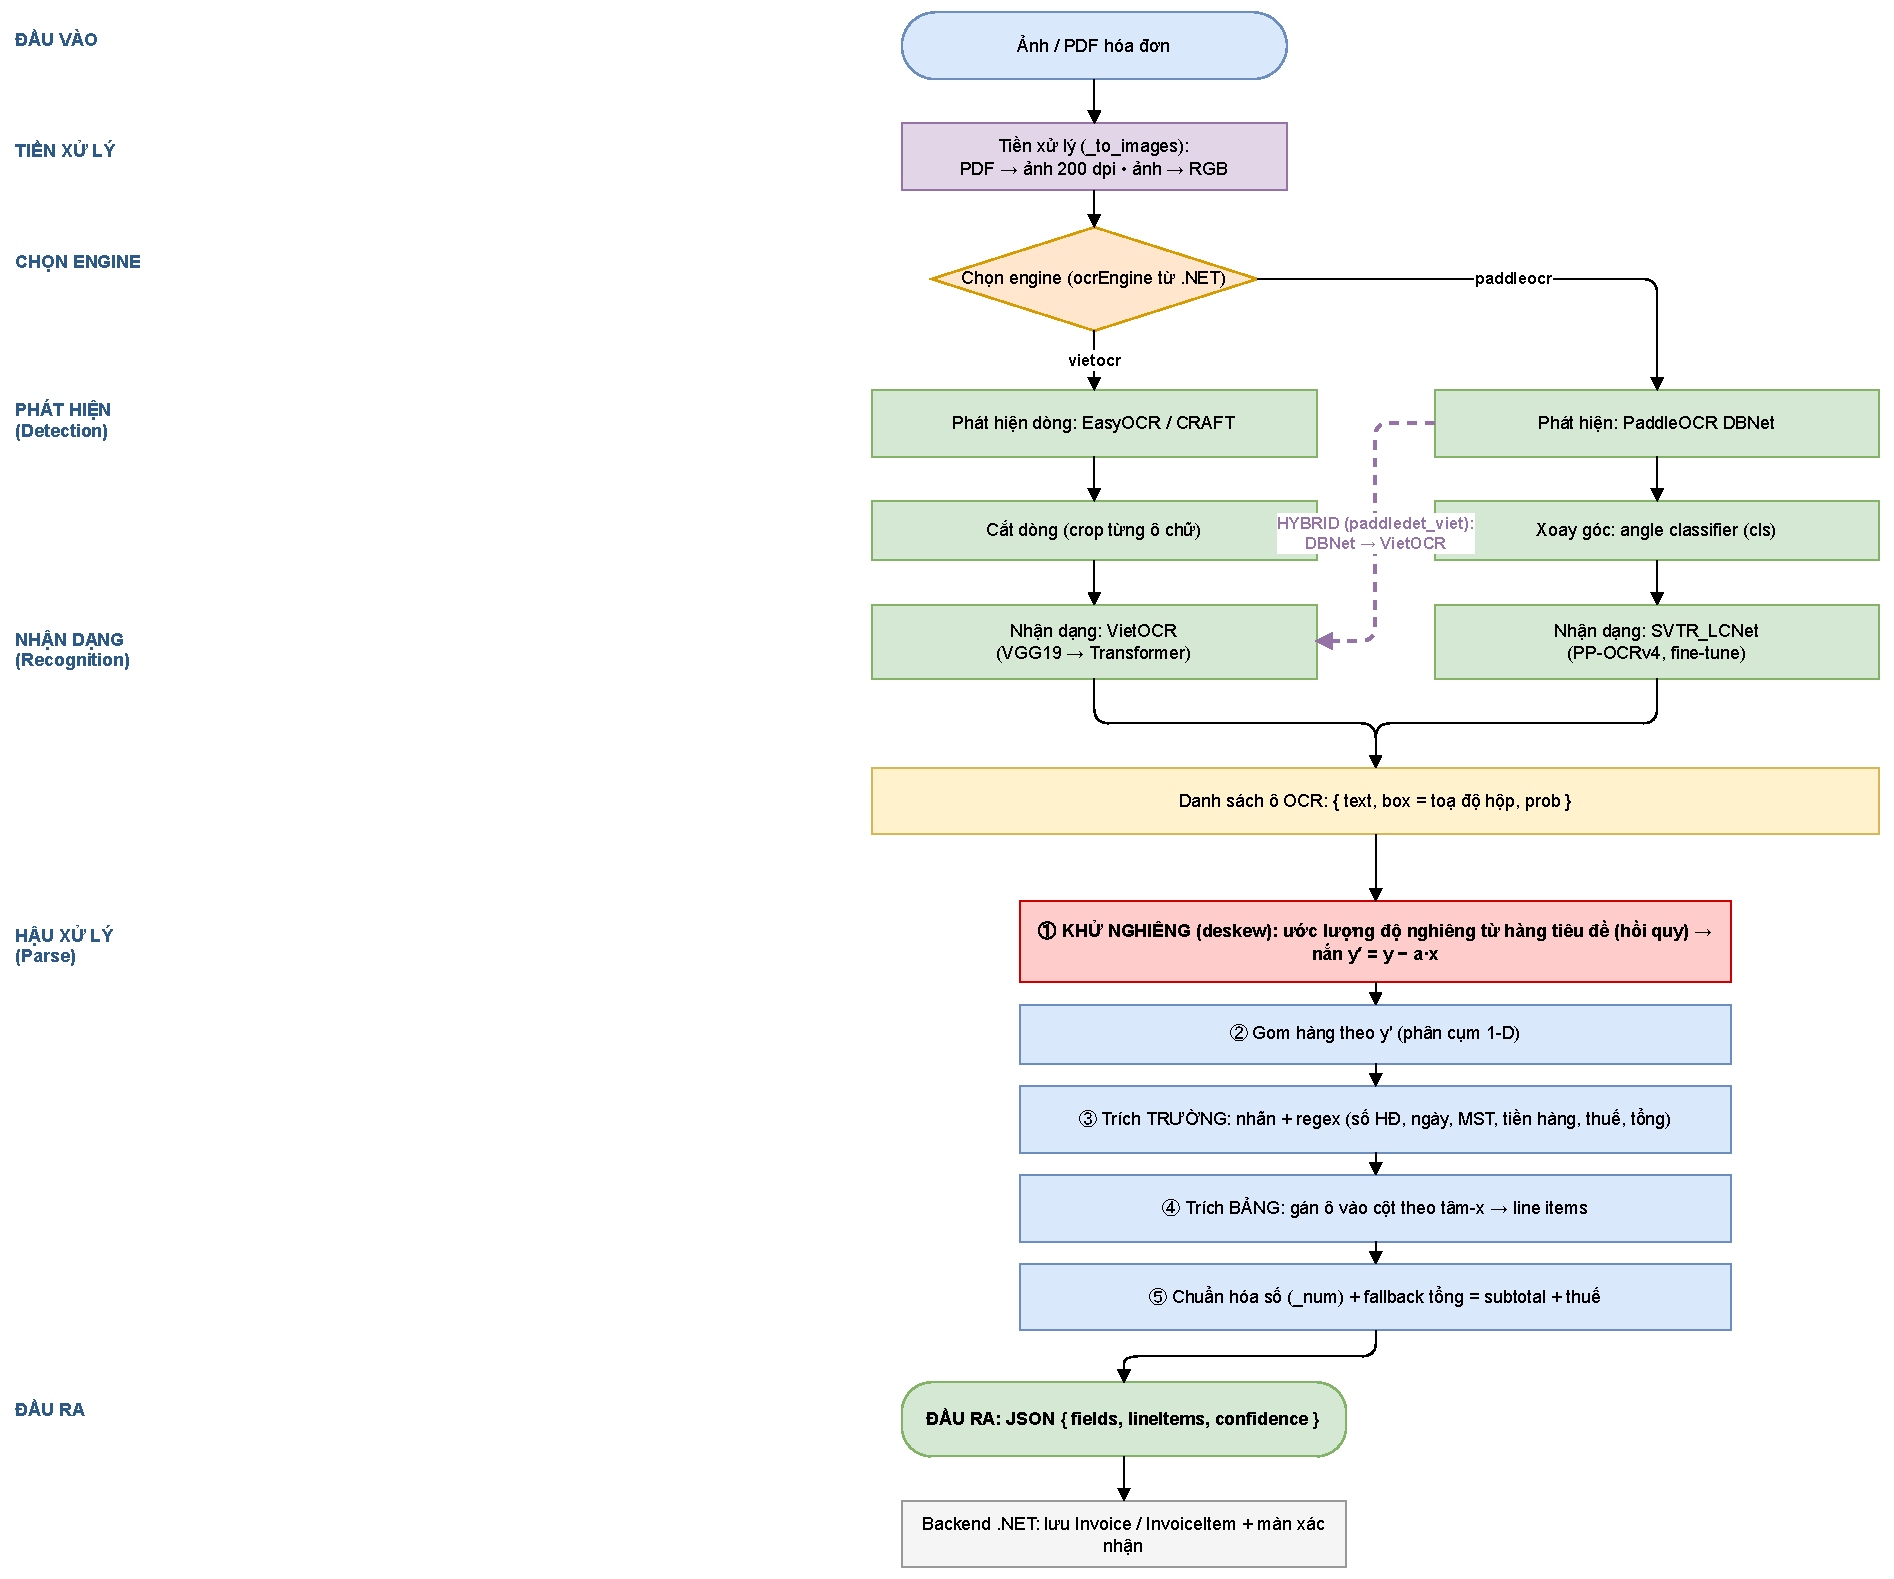
\includegraphics[width=\linewidth,height=0.82\textheight,keepaspectratio]{images/img35.pdf}
\caption*{\small Hình 4.24. Luồng xử lý AI end-to-end của dịch vụ OCR: các lớp xử lý và vị trí bước khử nghiêng.}
\addcontentsline{lof}{figure}{Hình 4.24. Luồng xử lý AI end-to-end của dịch vụ OCR: các lớp xử lý và vị trí bước khử nghiêng.}
\end{figure}
\subsubsection*{h) Biến thể hybrid: Paddle DBNet (phát hiện) + VietOCR (nhận dạng)}
\textbf{Ý tưởng. }Từ kết quả ở mục d), VietOCR cho độ chính xác nhận dạng cao nhất trong ba engine, trong khi bộ phát hiện DBNet của PaddleOCR (đã fine-tune) tốt hơn CRAFT của EasyOCR — vốn không được fine-tune và là nút cổ chai của pipeline vietocr. Vì vậy đề tài thử nghiệm thêm một biến thể hybrid (engine paddledet\_viet) ghép hai điểm mạnh: dùng DBNet để phát hiện dòng, rồi đưa từng vùng vào VietOCR để nhận dạng.

\textbf{Cơ chế ghép. }Do DBNet trả về đa giác bốn điểm (có thể xoay, nghiêng), lớp ghép thực hiện phép biến đổi phối cảnh để đưa mỗi vùng về ảnh dòng nằm ngang (tương tự hàm get\_rotate\_crop\_image của PaddleOCR) trước khi VietOCR đọc. Kết quả trả về cùng định dạng danh sách ô (văn bản, hộp bao, độ tin cậy) nên tái sử dụng nguyên vẹn bộ hậu xử lý ở mục f và g (khử nghiêng, trích trường và bảng).

\textbf{Phân tích ablation. }So sánh paddleocr (DBNet + Paddle SVTR) với paddledet\_viet (DBNet + VietOCR) là một ablation giữ nguyên detector, chỉ thay recognizer, do đó cô lập đúng ảnh hưởng của tầng nhận dạng. Cần lưu ý: phép đánh giá nhận dạng ở mục d) chạy trên các dòng đã cắt sẵn (ground-truth) nên không phụ thuộc detector; ở mức này biến thể hybrid dùng recognizer VietOCR nên có độ chính xác nhận dạng trùng với cột VietOCR (cao nhất). Khác biệt thực sự của hybrid nằm ở tầng phát hiện: DBNet fine-tune cắt dòng tốt và ổn định hơn CRAFT, nên khi chạy end-to-end trên hóa đơn cả trang, hybrid được kỳ vọng vượt pipeline vietocr (CRAFT + VietOCR) nhờ detector mạnh hơn, đồng thời giữ chất lượng đọc của VietOCR. Việc đối chiếu end-to-end trên từng hóa đơn được thực hiện bằng công cụ so sánh ba pipeline (mục g).

\textbf{Đánh đổi và lựa chọn. }Bù lại các ưu điểm trên, hybrid phải nạp đồng thời hai framework (PaddlePaddle và PyTorch) nên tốn bộ nhớ hơn; VietOCR nhận dạng theo từng dòng thay vì theo lô như SVTR nên chậm hơn; và triển khai một dịch vụ dùng hai framework cũng phức tạp hơn PaddleOCR hợp nhất. Vì vậy hệ thống chọn PaddleOCR làm engine mặc định cho vận hành, còn biến thể hybrid được cung cấp như một tùy chọn (paddledet\_viet) phục vụ đối chiếu và các tình huống ưu tiên độ chính xác nhận dạng hơn tốc độ.

\phantomsection
\subsection*{4.2.8. Khảo sát các giải pháp AI OCR khác và lý do lựa chọn}
\addcontentsline{toc}{subsection}{4.2.8. Khảo sát các giải pháp AI OCR khác và lý do lựa chọn}
Bóc tách hóa đơn bằng AI là bài toán đã trưởng thành, có nhiều giải pháp thương mại và mã nguồn mở. Trước khi tự xây dựng engine, nhóm đã khảo sát ba nhóm giải pháp phổ biến để làm căn cứ lựa chọn. Tất cả ảnh minh chứng dưới đây là ảnh chụp màn hình trang chính thức của từng sản phẩm, kèm đường dẫn nguồn ngay bên dưới; các số liệu giá tham khảo tại thời điểm khảo sát (07/2026).

\textbf{a) Nhóm dịch vụ đám mây (Cloud OCR/IDP API).} Đây là các API trả tiền theo lượt gọi, độ chính xác cao và không phải tự vận hành hạ tầng, nhưng dữ liệu phải gửi ra máy chủ bên thứ ba và chi phí tăng theo sản lượng:
\begin{itemize}[leftmargin=1.4em,itemsep=1pt,topsep=2pt]
  \item \textbf{Google Cloud Vision / Document AI} (Hình 4.25): trích văn bản và tài liệu, giá cơ bản \textasciitilde{}1,5 USD/1.000 trang, bản trích cấu trúc (Document AI) cao hơn nhiều; miễn phí 1.000 đơn vị/tháng.
  \item \textbf{Azure AI Document Intelligence} (Hình 4.26): có sẵn mô hình hóa đơn dựng sẵn (prebuilt-invoice), giá trích cấu trúc \textasciitilde{}10 USD/1.000 trang; miễn phí 500 trang/tháng.
  \item \textbf{Amazon Textract} (Hình 4.27): trích chữ, bảng, biểu mẫu; DetectDocumentText \textasciitilde{}1,5 USD/1.000 trang, còn AnalyzeDocument (bảng/biểu mẫu) lên tới \textasciitilde{}65 USD/1.000 trang.
\end{itemize}

\begin{figure}[H]\centering
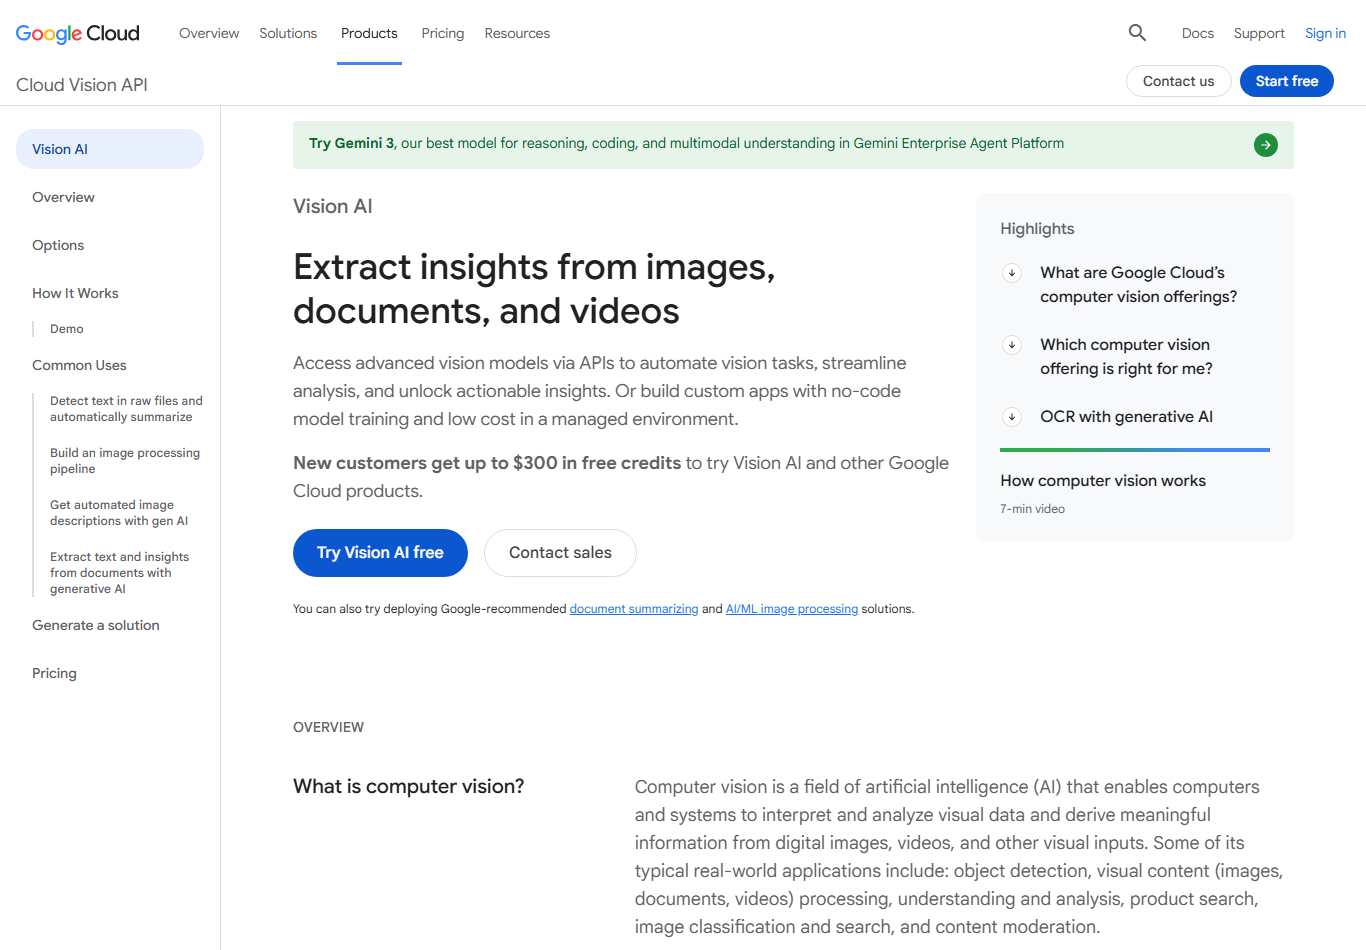
\includegraphics[width=\linewidth,height=0.4\textheight,keepaspectratio]{images/ocr_google.png}
\caption*{\small Hình 4.25. Google Cloud Vision AI — trích xuất văn bản/tài liệu qua API đám mây}
\addcontentsline{lof}{figure}{Hình 4.25. Google Cloud Vision AI (API đám mây)}
\end{figure}
\noindent\textit{\small Nguồn: \url{https://cloud.google.com/vision} (truy cập 07/2026).}

\begin{figure}[H]\centering
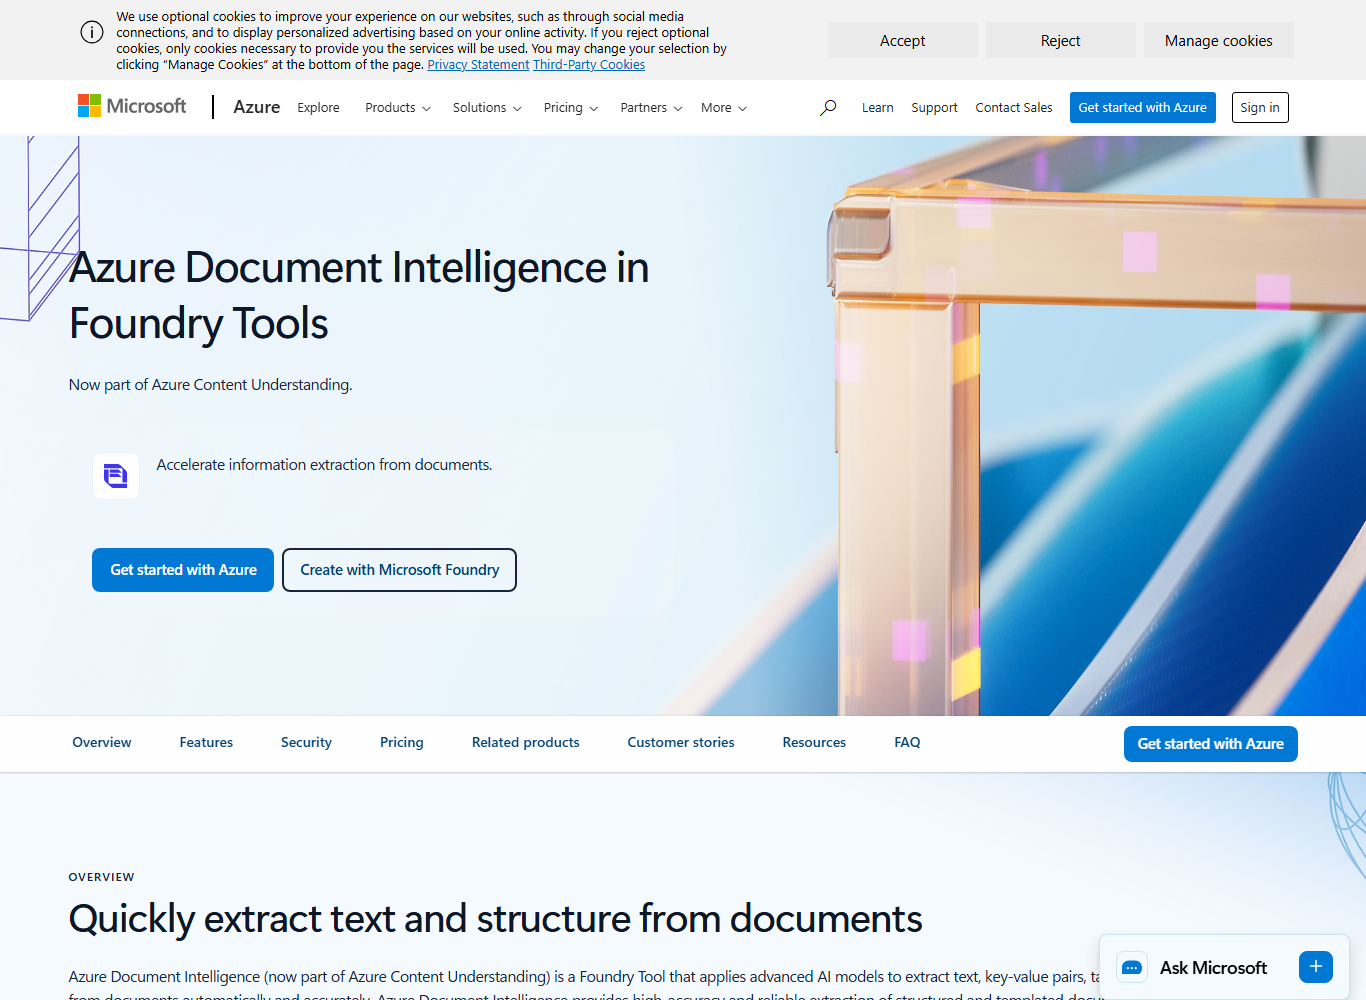
\includegraphics[width=\linewidth,height=0.4\textheight,keepaspectratio]{images/ocr_azure.png}
\caption*{\small Hình 4.26. Azure AI Document Intelligence — mô hình hóa đơn dựng sẵn}
\addcontentsline{lof}{figure}{Hình 4.26. Azure AI Document Intelligence}
\end{figure}
\noindent\textit{\small Nguồn: \url{https://azure.microsoft.com/en-us/products/ai-services/ai-document-intelligence} (truy cập 07/2026).}

\begin{figure}[H]\centering
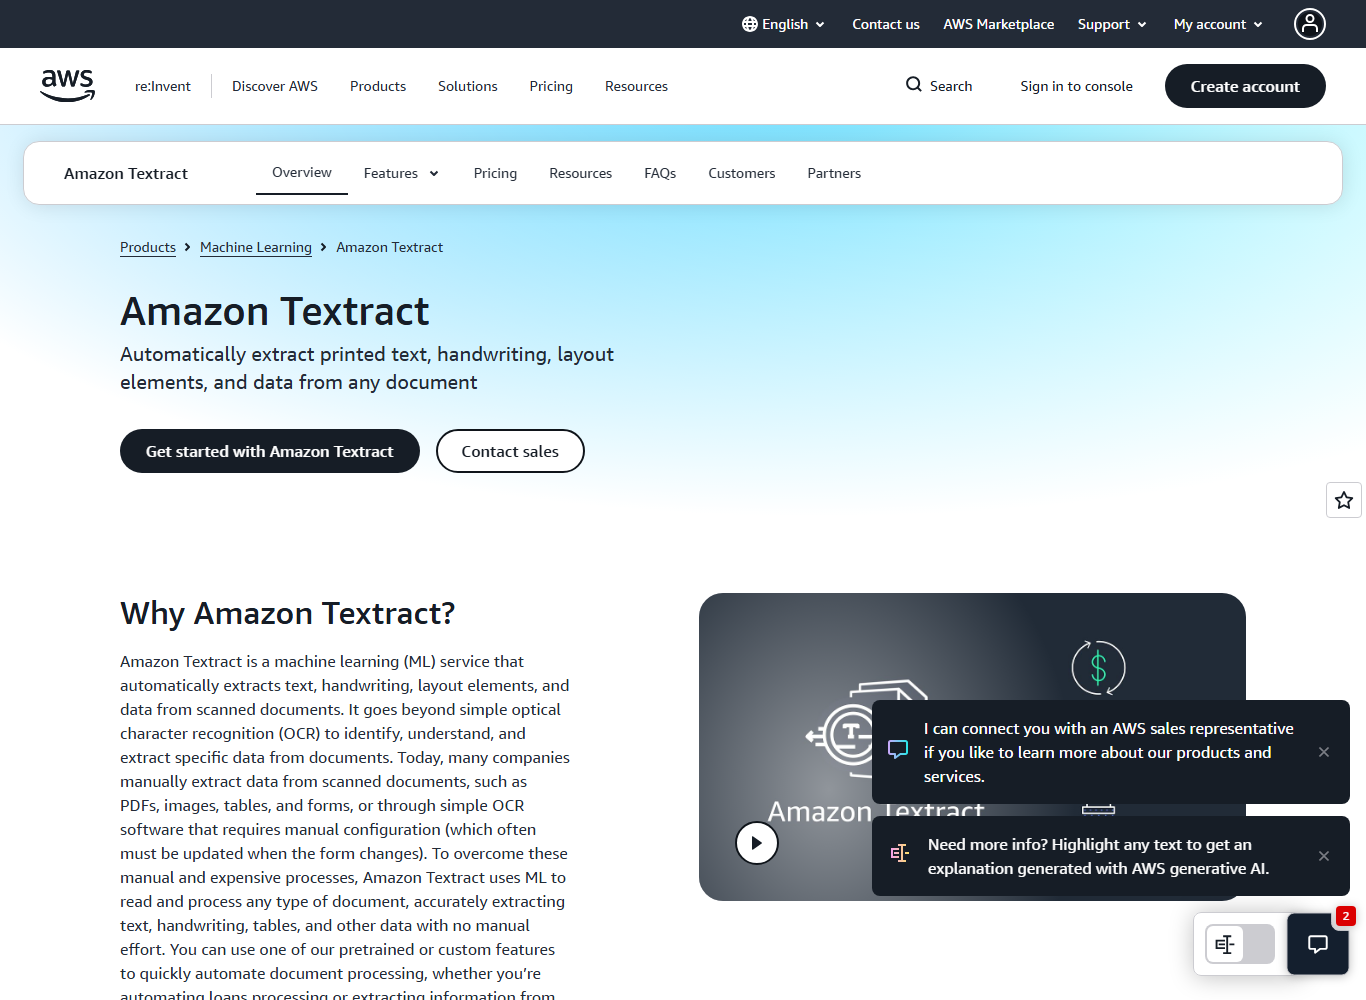
\includegraphics[width=\linewidth,height=0.4\textheight,keepaspectratio]{images/ocr_textract.png}
\caption*{\small Hình 4.27. Amazon Textract — trích chữ, bảng và biểu mẫu từ tài liệu}
\addcontentsline{lof}{figure}{Hình 4.27. Amazon Textract}
\end{figure}
\noindent\textit{\small Nguồn: \url{https://aws.amazon.com/textract/} (truy cập 07/2026).}

\textbf{b) Nhóm SDK thương mại cài tại chỗ.} Tiêu biểu là \textbf{ABBYY FineReader Engine} (Hình 4.28) -- bộ SDK OCR lâu đời, độ chính xác cao, chạy được on-premise (bảo mật tốt) nhưng chi phí bản quyền lớn và mô hình đóng, không tùy biến sâu cho hóa đơn tiếng Việt.

\begin{figure}[H]\centering
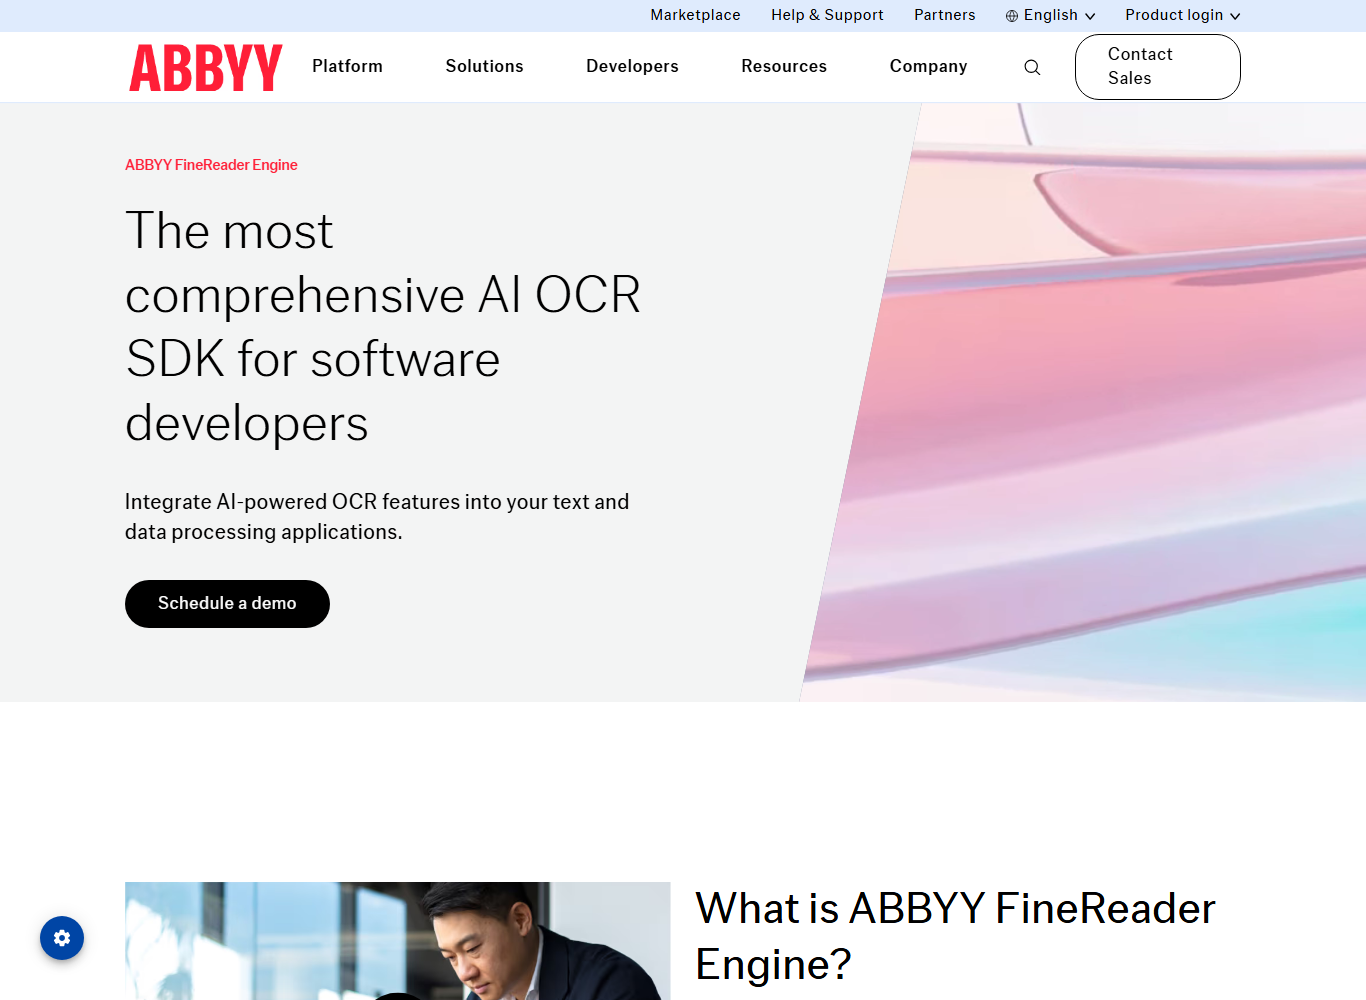
\includegraphics[width=\linewidth,height=0.4\textheight,keepaspectratio]{images/ocr_abbyy.png}
\caption*{\small Hình 4.28. ABBYY FineReader Engine — SDK OCR thương mại cài tại chỗ}
\addcontentsline{lof}{figure}{Hình 4.28. ABBYY FineReader Engine (SDK thương mại)}
\end{figure}
\noindent\textit{\small Nguồn: \url{https://www.abbyy.com/ocr-sdk/} (truy cập 07/2026).}

\textbf{c) Nhóm mã nguồn mở, tự triển khai.} Miễn phí, chạy offline, tùy biến và fine-tune được:
\begin{itemize}[leftmargin=1.4em,itemsep=1pt,topsep=2pt]
  \item \textbf{Tesseract} (Hình 4.29): engine mã nguồn mở lâu đời của Google; đọc tài liệu in tốt nhưng yếu với hóa đơn tiếng Việt bố cục phức tạp nếu không huấn luyện lại, và chậm hơn (CPU \textasciitilde{}25 trang/phút).
  \item \textbf{PaddleOCR} (Hình 4.30): bộ công cụ OCR nhẹ, hợp nhất phát hiện + nhận dạng, hỗ trợ 100+ ngôn ngữ, fine-tune được cả hai tầng, nhanh (GPU \textasciitilde{}120 trang/phút) -- đây là engine nhóm chọn, kết hợp thêm \textbf{VietOCR} (recognizer mạnh về dấu tiếng Việt) và bộ phát hiện CRAFT của EasyOCR.
\end{itemize}

\begin{figure}[H]\centering
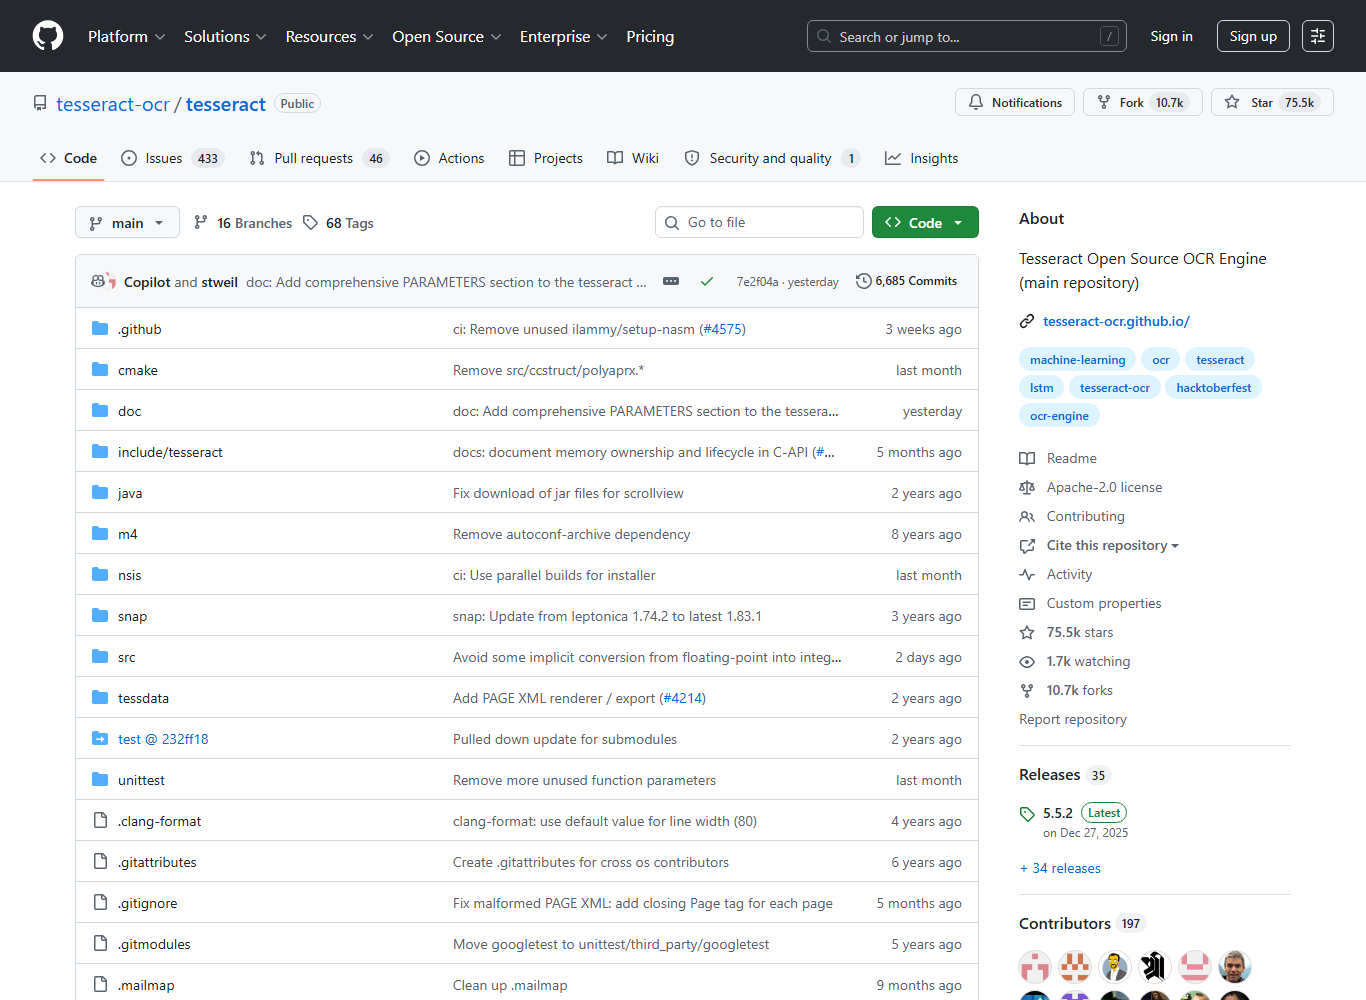
\includegraphics[width=\linewidth,height=0.4\textheight,keepaspectratio]{images/ocr_tesseract.png}
\caption*{\small Hình 4.29. Tesseract OCR (mã nguồn mở) trên GitHub}
\addcontentsline{lof}{figure}{Hình 4.29. Tesseract OCR (mã nguồn mở)}
\end{figure}
\noindent\textit{\small Nguồn: \url{https://github.com/tesseract-ocr/tesseract} (truy cập 07/2026).}

\begin{figure}[H]\centering
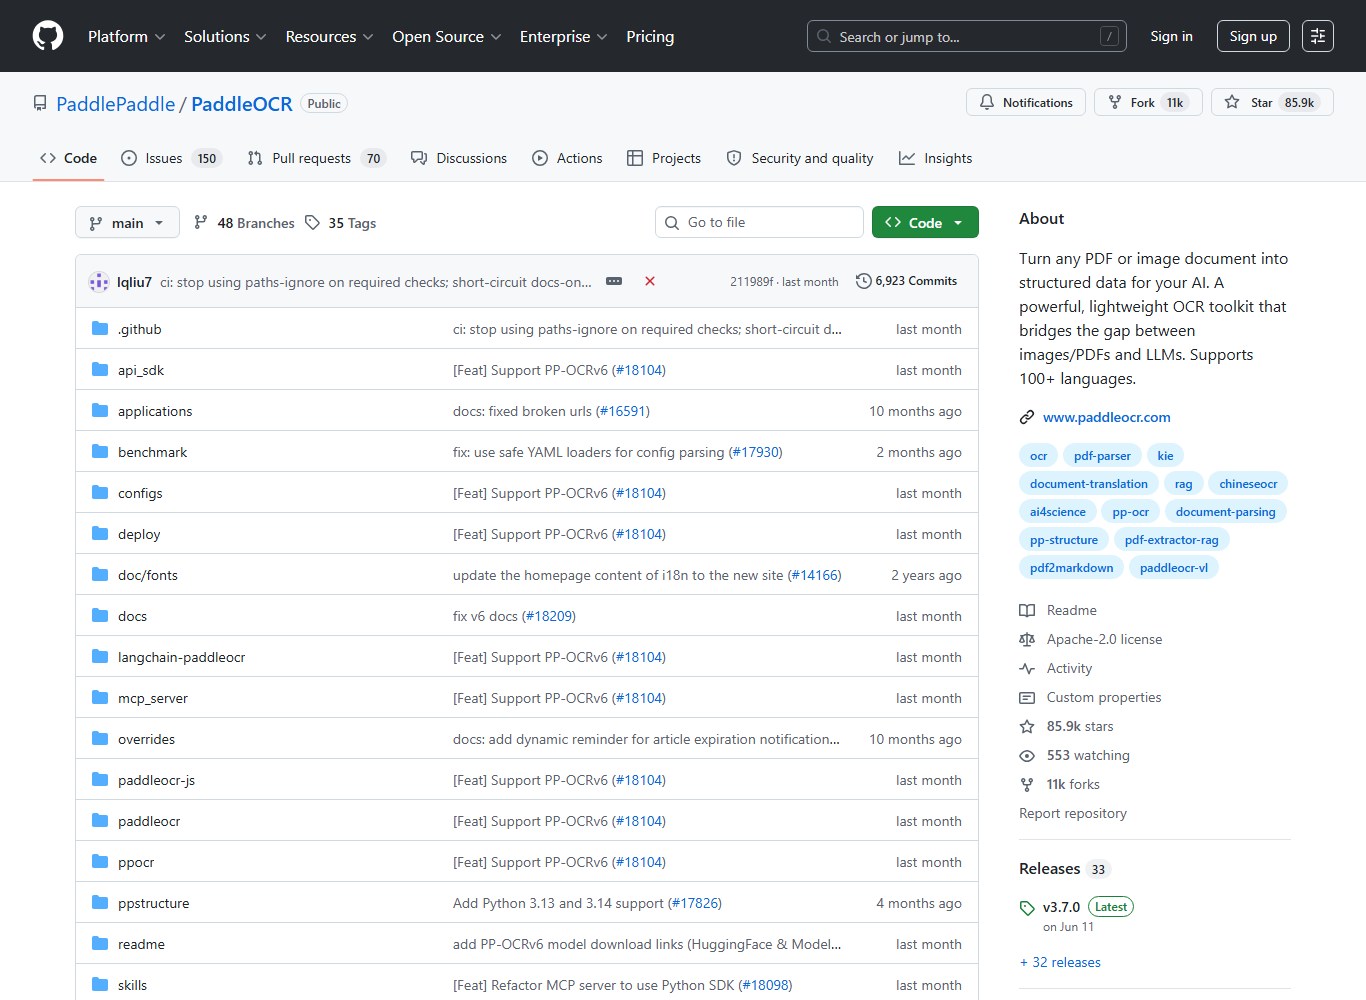
\includegraphics[width=\linewidth,height=0.4\textheight,keepaspectratio]{images/ocr_paddle.png}
\caption*{\small Hình 4.30. PaddleOCR (mã nguồn mở, Apache-2.0, \textasciitilde{}86k sao GitHub) -- engine nhóm lựa chọn}
\addcontentsline{lof}{figure}{Hình 4.30. PaddleOCR (mã nguồn mở) -- engine được chọn}
\end{figure}
\noindent\textit{\small Nguồn: \url{https://github.com/PaddlePaddle/PaddleOCR} (truy cập 07/2026).}

\textbf{Bảng xếp hạng, so sánh các giải pháp.} Nhóm chấm điểm theo các tiêu chí quan trọng với bài toán (đọc hóa đơn tiếng Việt trong hệ quản lý tòa nhà) và với yêu cầu của một đồ án tốt nghiệp:

\begin{landscape}\begin{center}{\footnotesize\singlespacing\renewcommand{\arraystretch}{1.25}
\begin{tabular}{|>{\raggedright\arraybackslash}p{3.1cm}|>{\raggedright\arraybackslash}p{2.3cm}|>{\raggedright\arraybackslash}p{2.6cm}|>{\raggedright\arraybackslash}p{2.6cm}|>{\raggedright\arraybackslash}p{2.5cm}|>{\raggedright\arraybackslash}p{2.5cm}|>{\raggedright\arraybackslash}p{2.4cm}|}
\hline
\textbf{Giải pháp} & \textbf{Loại} & \textbf{Độ chính xác HĐ tiếng Việt} & \textbf{Chi phí} & \textbf{Tự chủ / Offline \& bảo mật} & \textbf{Fine-tune trên dữ liệu riêng} & \textbf{Phù hợp đồ án} \\ \hline
Google Vision / Document AI & Cloud API & Cao & Trả theo lượt (\textasciitilde{}1,5–nhiều USD/1k trang) & Không (gửi HĐ lên cloud) & Hạn chế (không sở hữu model) & Thấp \\ \hline
Azure Document Intelligence & Cloud API & Cao & \textasciitilde{}10 USD/1k trang (invoice) & Không / có container trả phí & Custom model (trả phí) & Thấp \\ \hline
Amazon Textract & Cloud API & Cao & \textasciitilde{}1,5–65 USD/1k trang & Không & Không & Thấp \\ \hline
ABBYY FineReader & SDK thương mại & Cao & Bản quyền lớn & Có (on-prem) & Hạn chế (đóng) & Thấp \\ \hline
Tesseract & Mã nguồn mở & Trung bình–thấp & Miễn phí & Có & Có (khó) & Trung bình \\ \hline
\textbf{PaddleOCR (chọn)} & Mã nguồn mở & \textbf{Cao} (0,893 seq; 65 ms) & Miễn phí & \textbf{Có} & \textbf{Có (det+rec)} & \textbf{Rất phù hợp} \\ \hline
\textbf{VietOCR (chọn)} & Mã nguồn mở & \textbf{Rất cao} (1,000 seq) & Miễn phí & \textbf{Có} & \textbf{Có (rec)} & \textbf{Rất phù hợp} \\ \hline
\end{tabular}}\end{center}\end{landscape}
\noindent\textit{\small Nguồn số liệu giá: tổng hợp từ trang giá chính thức của Google Cloud Vision, Azure AI Document Intelligence và \url{https://aws.amazon.com/textract/pricing/} (07/2026); số liệu độ chính xác/tốc độ engine lấy từ thực nghiệm của nhóm ở mục 4.2.7.d.}

\textbf{Lý do lựa chọn PaddleOCR + VietOCR (tự triển khai).} Trên cơ sở khảo sát, nhóm chọn hướng \emph{tự triển khai mã nguồn mở} thay vì API đám mây hay SDK thương mại, vì:
\begin{itemize}[leftmargin=1.4em,itemsep=1pt,topsep=2pt]
  \item \textbf{Bảo mật dữ liệu:} hóa đơn chứa thông tin tài chính – thuế nhạy cảm của tòa nhà; giải pháp tự triển khai chạy \emph{offline}, dữ liệu không rời khỏi hệ thống, tránh rủi ro khi gửi lên máy chủ bên thứ ba.
  \item \textbf{Chi phí:} miễn phí bản quyền, không phát sinh phí theo lượt gọi – phù hợp khi số lượng hóa đơn lớn và ngân sách đồ án hạn chế (các API đám mây tính \textasciitilde{}1,5–65 USD/1.000 trang).
  \item \textbf{Fine-tune được trên dữ liệu tiếng Việt:} nhóm tự sinh dataset hóa đơn GTGT và fine-tune, đạt độ chính xác nhận dạng 99,64\% (PaddleOCR) và 100\% (VietOCR) trên tập val – điều mà các API/SDK đóng không cho phép tùy biến sâu (xem mục 4.2.7.d).
  \item \textbf{Chủ động và không phụ thuộc:} không lệ thuộc Internet hay nhà cung cấp (vendor lock-in), phù hợp môi trường vận hành tòa nhà.
  \item \textbf{Đúng tinh thần đồ án tốt nghiệp:} thể hiện năng lực \emph{xây dựng, huấn luyện và đánh giá} mô hình AI, thay vì chỉ gọi dịch vụ có sẵn.
\end{itemize}
Tóm lại, các giải pháp đám mây/thương mại chính xác và tiện nhưng đánh đổi chi phí, quyền riêng tư dữ liệu và khả năng tùy biến; hướng tự triển khai PaddleOCR + VietOCR đáp ứng tốt nhất các tiêu chí của đề tài.

\phantomsection
\section*{4.3. Nghiệp vụ Quản lý sự cố và SLA}
\addcontentsline{toc}{section}{4.3. Nghiệp vụ Quản lý sự cố và SLA}
\phantomsection
\subsection*{4.3.1. Đặt vấn đề và phạm vi}
\addcontentsline{toc}{subsection}{4.3.1. Đặt vấn đề và phạm vi}
Trong vận hành tòa nhà, sự cố (điện, nước, HVAC, thang máy, PCCC\ldots{}) phát sinh liên tục và cần được tiếp nhận, phân công, xử lý đúng cam kết thời gian (SLA). Phân hệ Quản lý sự cố (CM) số hóa toàn bộ quy trình từ báo sự cố đến đóng và đánh giá, đồng thời theo dõi tuân thủ SLA và leo thang khi trễ hạn.

\begin{itemize}[leftmargin=1.4em,itemsep=1pt,topsep=2pt]
  \item Tiếp nhận sự cố từ cư dân/kỹ thuật viên (ticket) theo loại và mức ưu tiên.
  \item Phân công kỹ thuật viên, cập nhật trạng thái, đính kèm ảnh trước/sau.
  \item Cấu hình SLA theo mức ưu tiên (thời gian phản hồi, thời gian giải quyết).
  \item Theo dõi hạn SLA, tự động leo thang khi sắp/đã quá hạn; SLA Dashboard.
  \item Đánh giá mức độ hài lòng của người báo sau khi đóng sự cố.
\end{itemize}
\phantomsection
\subsection*{4.3.2. Mối liên hệ với Base và các phân hệ khác}
\addcontentsline{toc}{subsection}{4.3.2. Mối liên hệ với Base và các phân hệ khác}
Nghiệp vụ Sự cố \& SLA khép kín chuỗi nghiệp vụ của phân hệ Quản lý tài sản - kế thừa dữ liệu tài sản, kho do chính tác giả xây dựng và sử dụng các dịch vụ nền tảng chung của nhóm:

\begin{itemize}[leftmargin=1.4em,itemsep=1pt,topsep=2pt]
  \item \textbf{Với Tài sản: }ticket gắn tài sản liên quan để truy vết thiết bị hỏng.
  \item \textbf{Với Kho/Mua sắm: }khi xử lý cần vật tư có thể xuất kho hoặc tạo đề xuất mua (PR).
  \item \textbf{Với Base: }phân quyền RBAC theo vai trò (cư dân/KTV/điều phối/quản lý); gửi thông báo khi phân công, sắp/đã quá hạn SLA.
\end{itemize}
\phantomsection
\subsection*{4.3.3. Phân tích yêu cầu chức năng}
\addcontentsline{toc}{subsection}{4.3.3. Phân tích yêu cầu chức năng}
\subsubsection*{a) Vòng đời và trạng thái sự cố}
Trạng thái ticket diễn tiến: Mới tiếp nhận $\rightarrow$ Chờ phân công $\rightarrow$ Đã phân công $\rightarrow$ Đang xử lý $\rightarrow$ Chờ vật tư (nếu thiếu) $\rightarrow$ Đã xử lý $\rightarrow$ Đã đóng. Mỗi lần đổi trạng thái được ghi vào lịch sử (TicketStatusHistory).

\subsubsection*{b) Loại sự cố, nguồn báo và mức ưu tiên}
Loại sự cố: Điện, Nước, HVAC, Thang máy, PCCC, Khác. Mỗi mức ưu tiên gắn với một cam kết SLA (thời gian phản hồi và giải quyết). Khi tạo ticket có thể để trống SLA để hệ thống tự áp theo mức ưu tiên.

\subsubsection*{c) Tiếp nhận, phân công và xử lý}
Quy trình: Báo sự cố (tạo ticket) $\rightarrow$ tiếp nhận \& phân công KTV (TicketAssignment) $\rightarrow$ KTV xử lý, cập nhật trạng thái, xuất vật tư/tạo PR nếu thiếu, chụp ảnh trước/sau (TicketAttachment) $\rightarrow$ đóng sự cố khi khắc phục xong. Luồng xử lý sự cố và giám sát SLA được minh họa ở Hình 4.31.

\begin{figure}[H]\centering

\includegraphics[width=\linewidth,height=0.82\textheight,keepaspectratio]{images/img36.pdf}
\caption*{\small Hình 4.31. Lưu đồ nghiệp vụ: Xử lý sự cố và giám sát SLA}
\addcontentsline{lof}{figure}{Hình 4.31. Lưu đồ nghiệp vụ: Xử lý sự cố và giám sát SLA}
\end{figure}
\subsubsection*{d) SLA và leo thang}
Cấu hình SLA (SlaConfig) định nghĩa thời gian phản hồi và giải quyết theo mức ưu tiên. Hệ thống theo dõi hạn SLA suốt quá trình; khi sắp/đã quá hạn sẽ leo thang và ghi nhật ký (SlaEscalationLog). Màn hình SLA Dashboard tổng hợp tỉ lệ tuân thủ, số ticket quá hạn.

\subsubsection*{e) Đánh giá mức độ hài lòng}
Sau khi đóng, người báo (cư dân) chấm sao mức độ hài lòng (TicketRating), phục vụ đánh giá chất lượng dịch vụ.

\phantomsection
\subsection*{4.3.4. Yêu cầu phi chức năng}
\addcontentsline{toc}{subsection}{4.3.4. Yêu cầu phi chức năng}
\begin{itemize}[leftmargin=1.4em,itemsep=1pt,topsep=2pt]
  \item Tính kịp thời: theo dõi và cảnh báo SLA theo thời gian thực.
  \item Truy vết đầy đủ: lịch sử trạng thái, phân công, đính kèm và leo thang.
\end{itemize}
\phantomsection
\subsection*{4.3.5. Thiết kế phân hệ}
\addcontentsline{toc}{subsection}{4.3.5. Thiết kế phân hệ}
\subsubsection*{a) Danh sách Use Case chính}
Các use case chính của phân hệ được thể hiện trên biểu đồ use case ở Hình 4.32 và liệt kê trong bảng dưới đây.

\begin{figure}[H]\centering
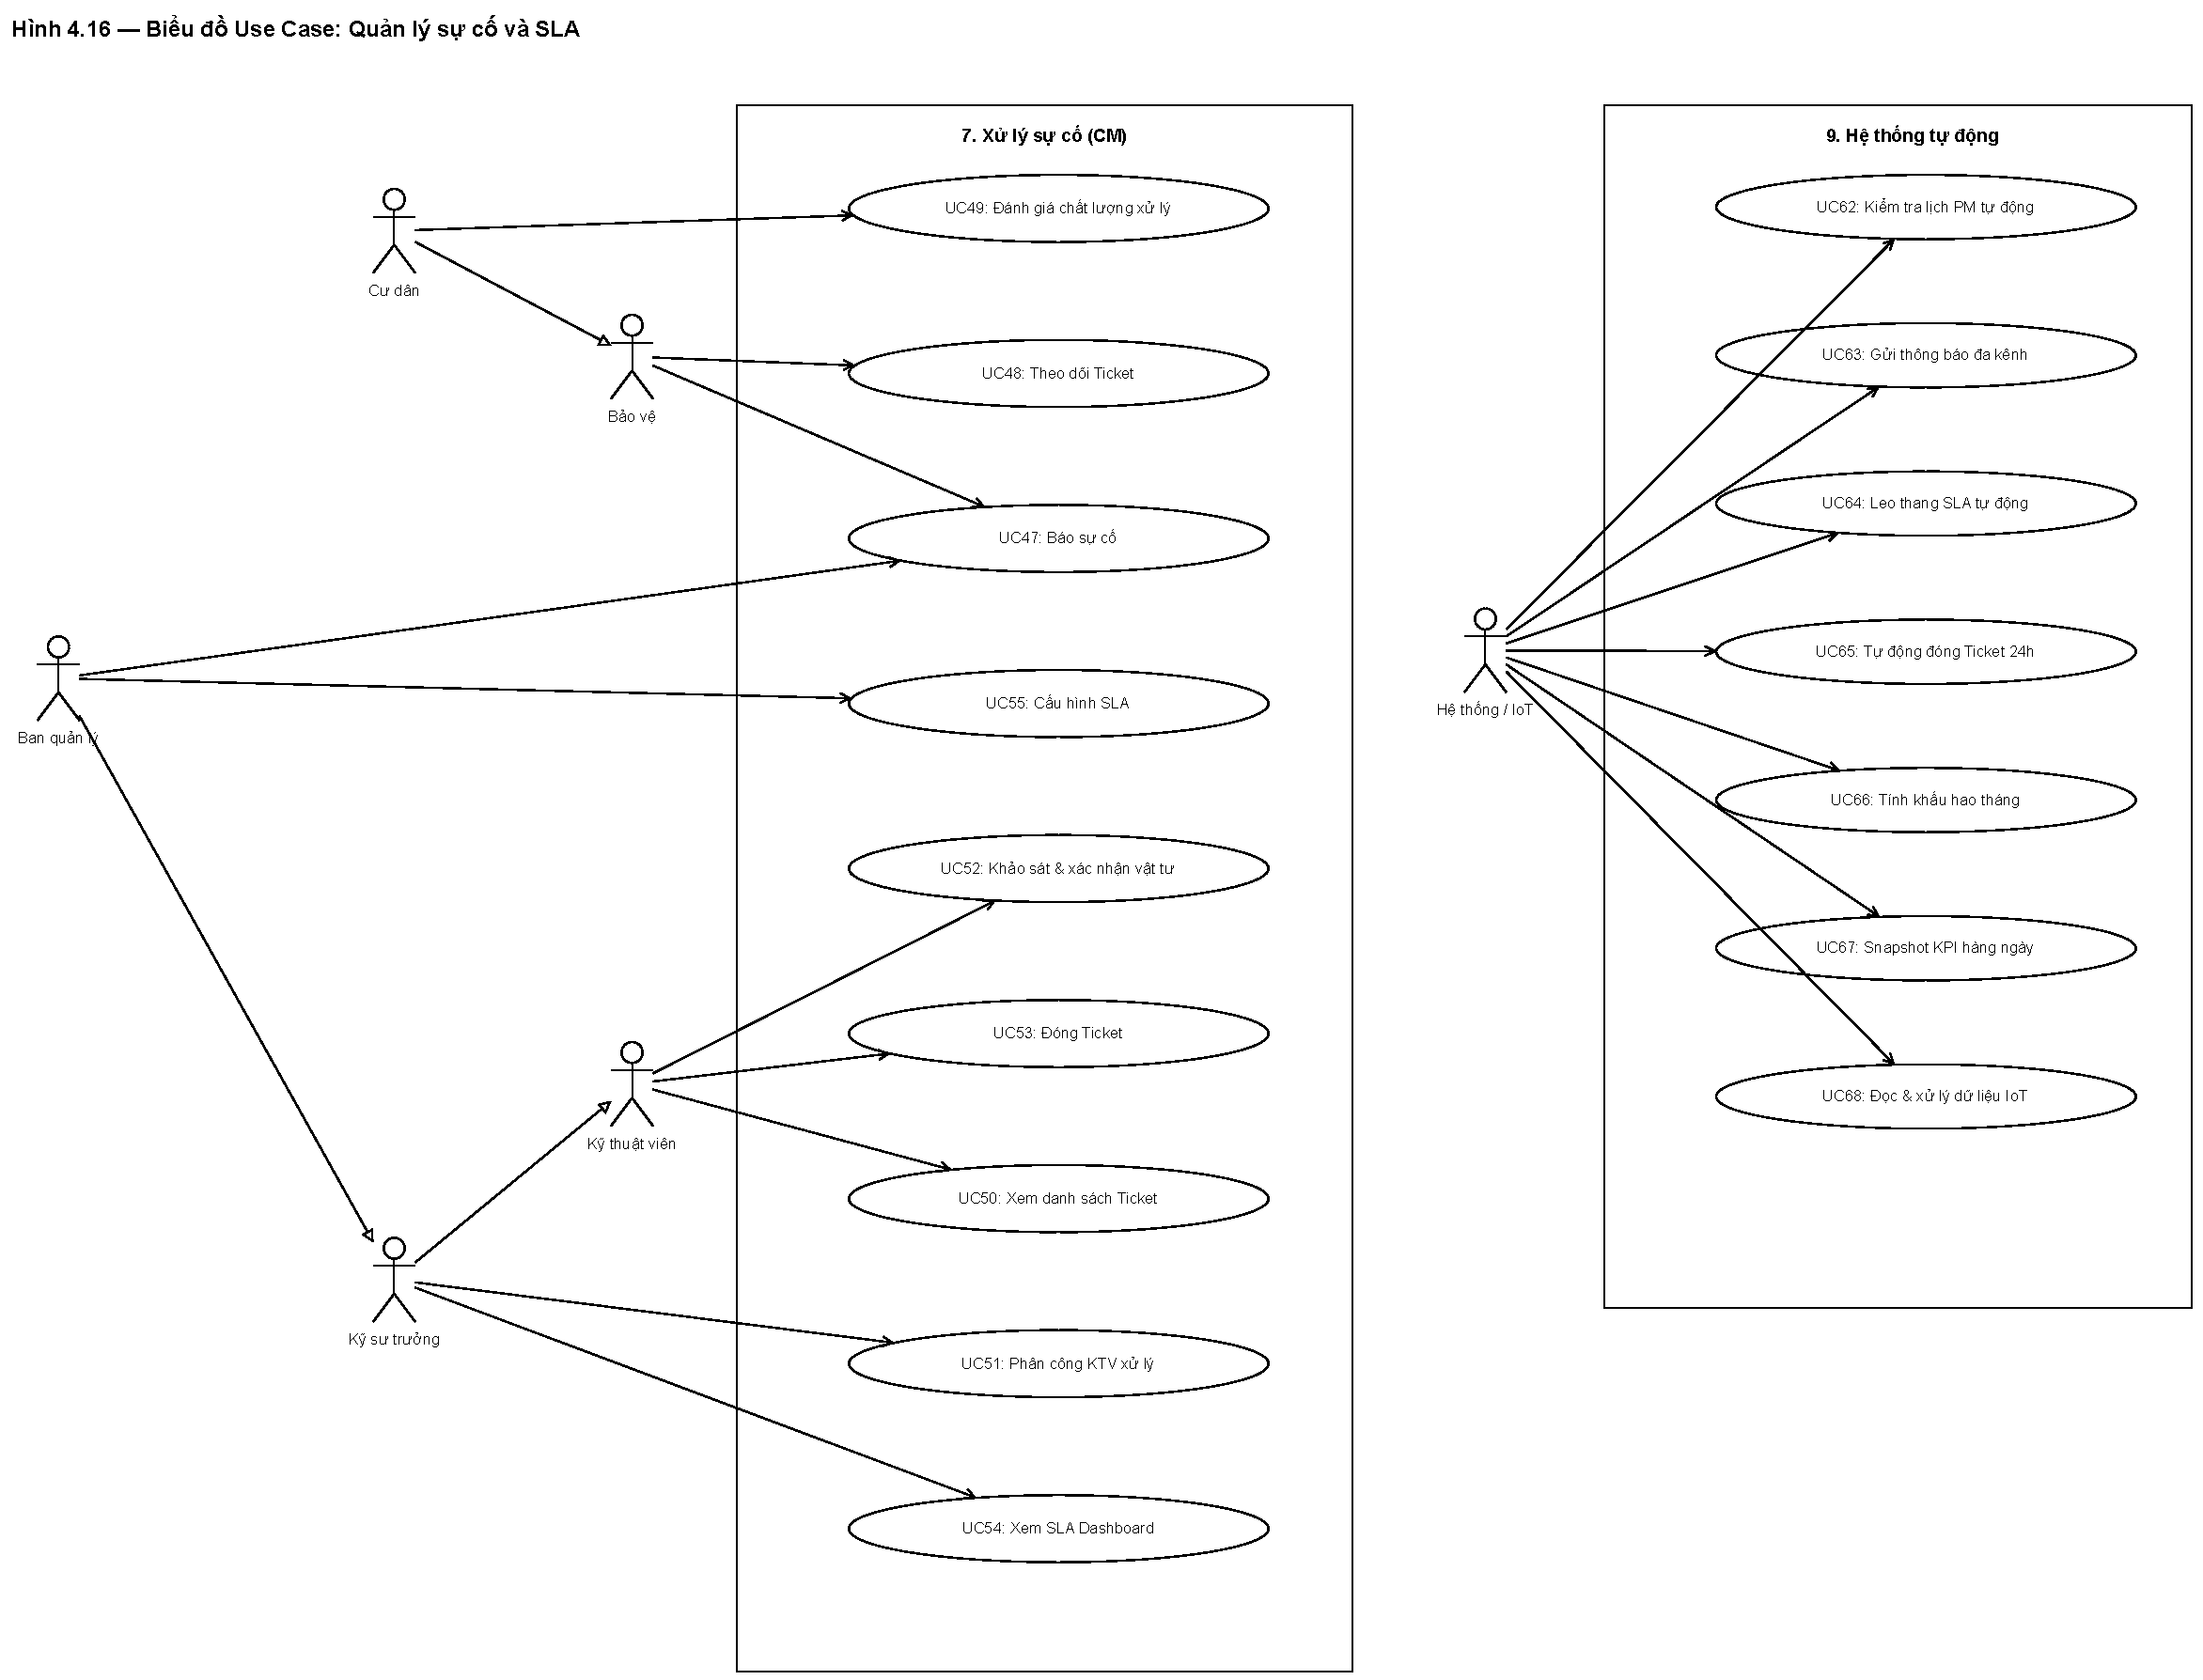
\includegraphics[width=\linewidth,height=0.82\textheight,keepaspectratio]{images/img37.pdf}
\caption*{\small Hình 4.32. Biểu đồ Use Case – Quản lý sự cố và SLA}
\addcontentsline{lof}{figure}{Hình 4.32. Biểu đồ Use Case – Quản lý sự cố và SLA}
\end{figure}
\begin{center}{\singlespacing\renewcommand{\arraystretch}{1.25}
\begin{tabular}{|>{\raggedright\arraybackslash}p{\dimexpr\linewidth/3-2\tabcolsep-\arrayrulewidth\relax}|>{\raggedright\arraybackslash}p{\dimexpr\linewidth/3-2\tabcolsep-\arrayrulewidth\relax}|>{\raggedright\arraybackslash}p{\dimexpr\linewidth/3-2\tabcolsep-\arrayrulewidth\relax}|}
\hline
\textbf{Mã UC} & \textbf{Use case} & \textbf{Tác nhân} \\ \hline
UC-CM-01 & Báo sự cố (tạo ticket) & Cư dân/​KTV \\ \hline
UC-CM-02 & Tiếp nhận \& phân công KTV & Điều phối \\ \hline
UC-CM-03 & Xử lý \& cập nhật trạng thái, đính kèm ảnh & KTV \\ \hline
UC-CM-04 & Cấu hình \& theo dõi SLA, leo thang & Quản lý/Hệ thống \\ \hline
UC-CM-05 & Đánh giá mức độ hài lòng & Cư dân \\ \hline
\end{tabular}}\end{center}
\subsubsection*{b) Sơ đồ trạng thái (state machine) của ticket}
Vòng đời trạng thái của một ticket sự cố được thể hiện ở Hình 4.33, trong đó trạng thái "Đang xử lý" có thể chuyển sang "Chờ vật tư" khi thiếu vật tư và quay lại khi đã có.

\begin{figure}[H]\centering
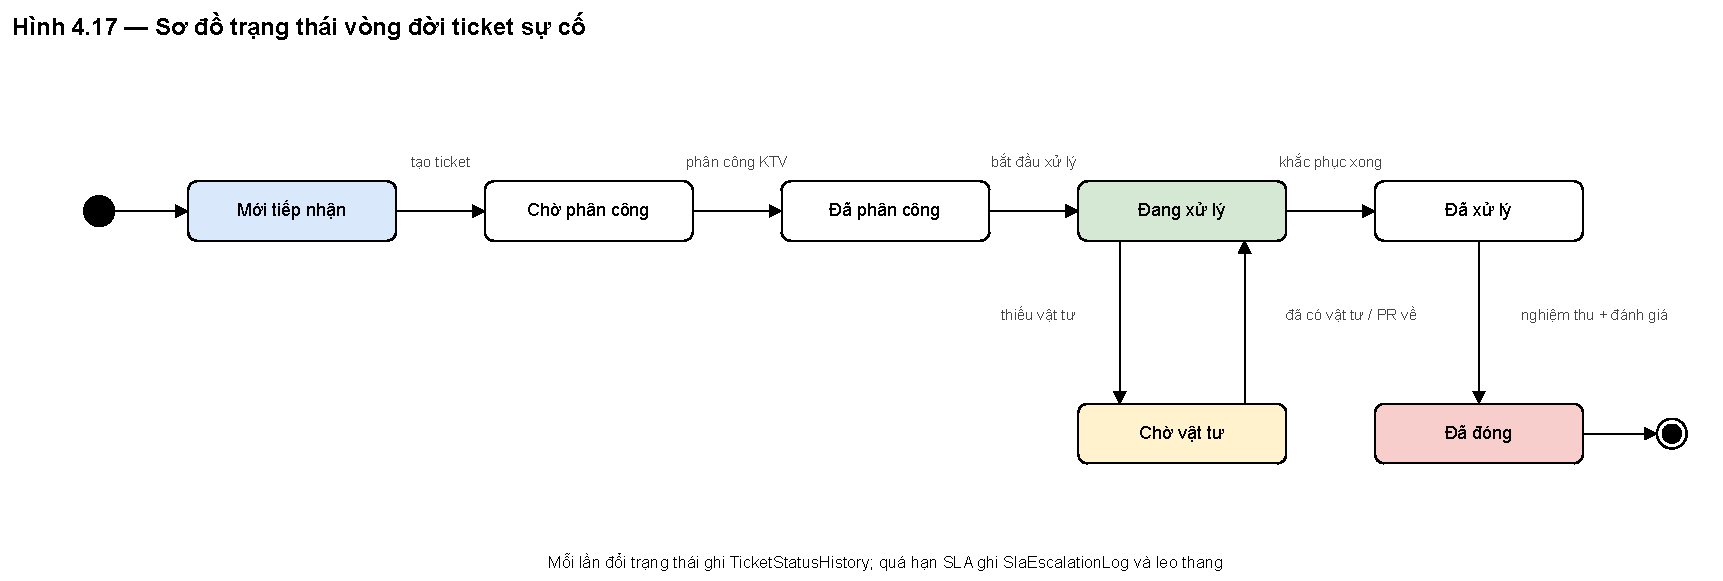
\includegraphics[width=\linewidth,height=0.82\textheight,keepaspectratio]{images/img38.pdf}
\caption*{\small Hình 4.33. Sơ đồ trạng thái vòng đời ticket sự cố}
\addcontentsline{lof}{figure}{Hình 4.33. Sơ đồ trạng thái vòng đời ticket sự cố}
\end{figure}
\begin{figure}[H]\centering

\includegraphics[width=\linewidth,height=0.82\textheight,keepaspectratio]{images/img39.png}
\caption*{\small Hình 4.34. Sơ đồ thực thể – liên kết (ERD) phân hệ Quản lý sự cố \& SLA}
\addcontentsline{lof}{figure}{Hình 4.34. Sơ đồ thực thể – liên kết (ERD) phân hệ Quản lý sự cố \& SLA}
\end{figure}
\subsubsection*{c) Thiết kế cơ sở dữ liệu (thực thể chính)}
\begin{center}{\singlespacing\renewcommand{\arraystretch}{1.25}
\begin{tabular}{|>{\raggedright\arraybackslash}p{\dimexpr\linewidth/2-2\tabcolsep-\arrayrulewidth\relax}|>{\raggedright\arraybackslash}p{\dimexpr\linewidth/2-2\tabcolsep-\arrayrulewidth\relax}|}
\hline
\textbf{Thực thể} & \textbf{Ý nghĩa} \\ \hline
Ticket & Sự cố: tiêu đề, loại, ưu tiên, nguồn báo, tài sản liên quan, trạng thái \\ \hline
TicketAssignment & Phân công kỹ thuật viên xử lý \\ \hline
TicketStatusHistory & Lịch sử thay đổi trạng thái \\ \hline
TicketAttachment & Ảnh/​tài liệu đính kèm (trước/​sau) \\ \hline
TicketRating & Đánh giá mức độ hài lòng \\ \hline
SlaConfig & Cấu hình SLA theo mức ưu tiên \\ \hline
SlaEscalationLog & Nhật ký leo thang khi trễ hạn \\ \hline
\end{tabular}}\end{center}
\subsubsection*{d) Thiết kế API}
\begin{center}{\singlespacing\renewcommand{\arraystretch}{1.25}
\begin{tabular}{|>{\raggedright\arraybackslash}p{\dimexpr\linewidth/2-2\tabcolsep-\arrayrulewidth\relax}|>{\raggedright\arraybackslash}p{\dimexpr\linewidth/2-2\tabcolsep-\arrayrulewidth\relax}|}
\hline
\textbf{Phương thức \& Endpoint} & \textbf{Chức năng} \\ \hline
POST /api/​asset/​ticket/​create & Tạo ticket sự cố \\ \hline
GET /api/​asset/​ticket/​get-all, get/\{id\} & Danh sách \& chi tiết \\ \hline
POST /api/​asset/​ticket/​assign & Phân công kỹ thuật viên \\ \hline
POST /api/​asset/​ticket/​change-status & Đổi trạng thái xử lý \\ \hline
POST /api/​asset/​ticket/​add-attachment & Đính kèm ảnh trước/​sau \\ \hline
POST /api/​asset/​ticket/​rate & Đánh giá hài lòng \\ \hline
GET .../get-status-history, get-escalation-logs/\{id\} & Lịch sử trạng thái \& leo thang \\ \hline
/api/​asset/​sla-config/* & CRUD cấu hình SLA \\ \hline
\end{tabular}}\end{center}
\phantomsection
\subsection*{4.3.6. Thiết kế giao diện}
\addcontentsline{toc}{subsection}{4.3.6. Thiết kế giao diện}
\begin{center}{\singlespacing\renewcommand{\arraystretch}{1.25}
\begin{tabular}{|>{\raggedright\arraybackslash}p{\dimexpr\linewidth/2-2\tabcolsep-\arrayrulewidth\relax}|>{\raggedright\arraybackslash}p{\dimexpr\linewidth/2-2\tabcolsep-\arrayrulewidth\relax}|}
\hline
\textbf{Route} & \textbf{Chức năng} \\ \hline
/tickets, /tickets/[id] & Danh sách \& chi tiết sự cố \\ \hline
/tickets/​new & Báo sự cố mới \\ \hline
/tickets/​sla-dashboard & Bảng theo dõi SLA \\ \hline
/my-tickets/[id], /settings/​sla & Sự cố của tôi \& cấu hình SLA \\ \hline
\end{tabular}}\end{center}
Một số màn hình tiêu biểu của phân hệ:

\begin{figure}[H]\centering
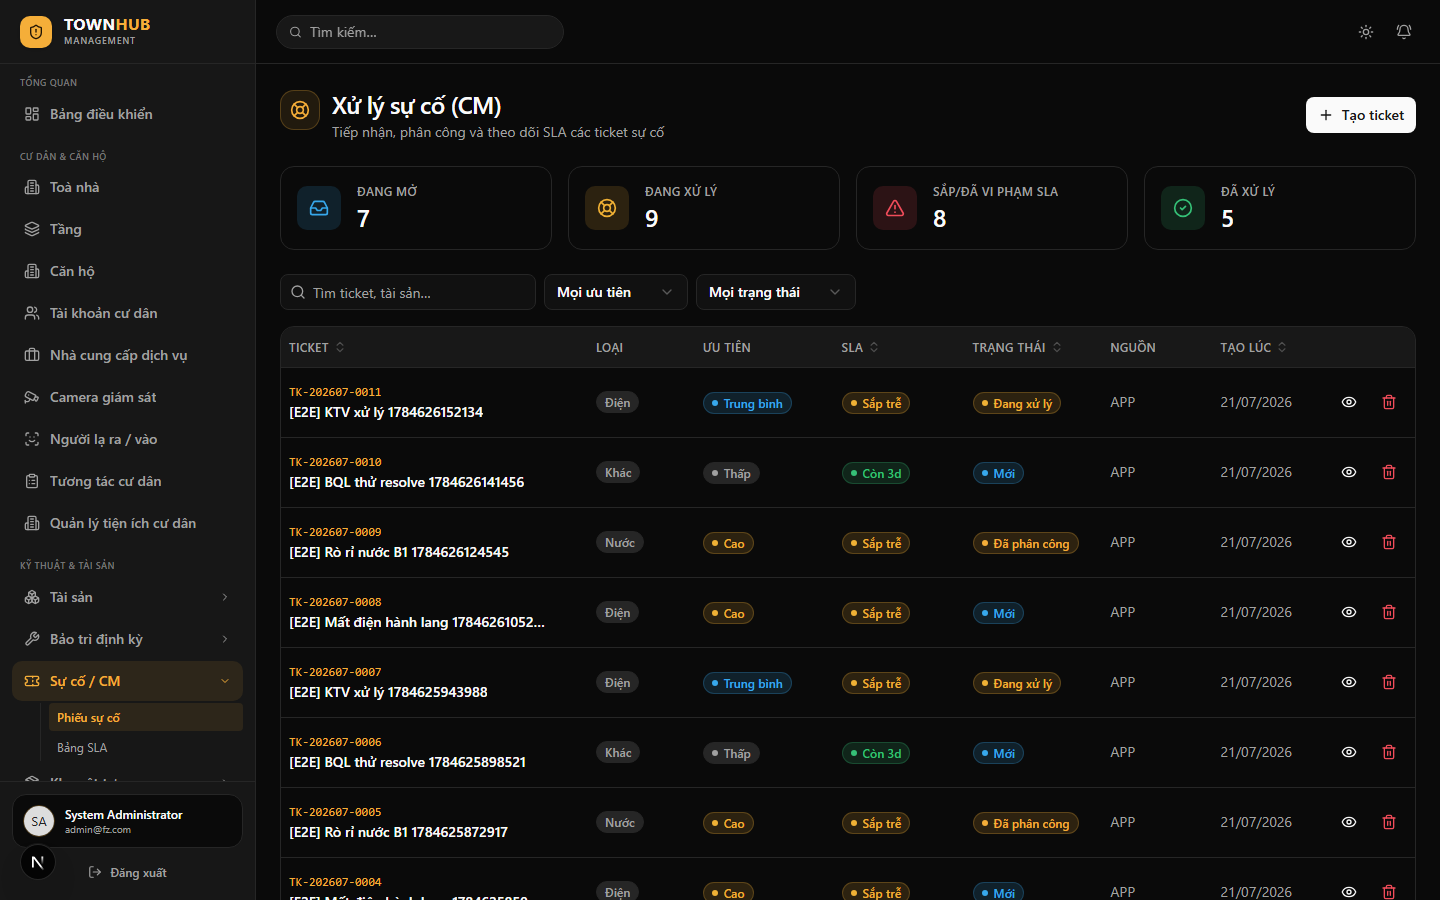
\includegraphics[width=\linewidth,height=0.82\textheight,keepaspectratio]{images/img40.png}
\caption*{\small Hình 4.35. Giao diện Danh sách phiếu sự cố (CM)}
\addcontentsline{lof}{figure}{Hình 4.35. Giao diện Danh sách phiếu sự cố (CM)}
\end{figure}
\begin{figure}[H]\centering
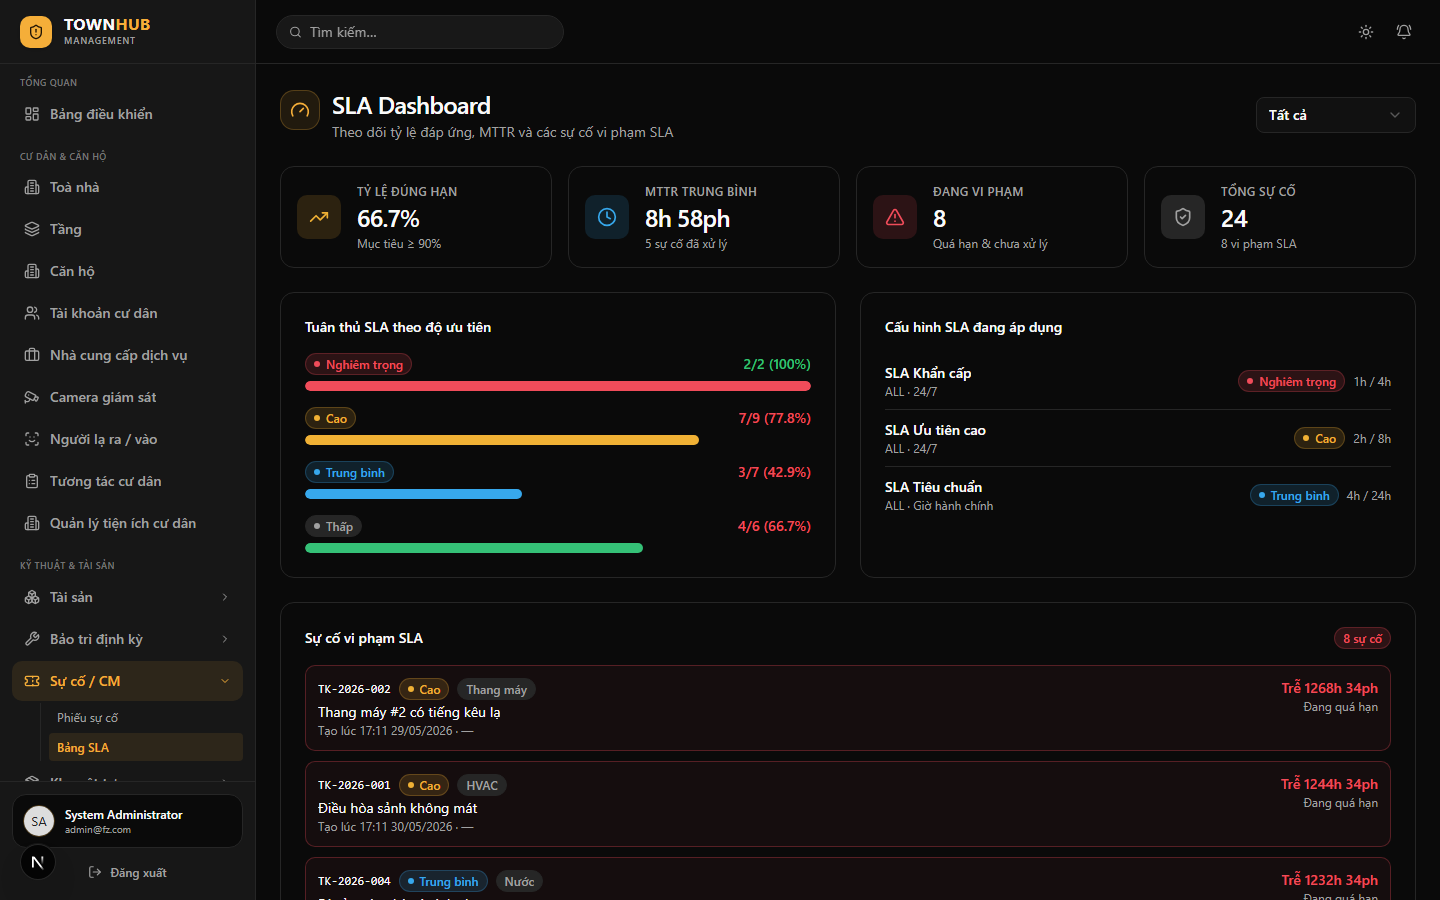
\includegraphics[width=\linewidth,height=0.82\textheight,keepaspectratio]{images/img41.png}
\caption*{\small Hình 4.36. Giao diện Bảng theo dõi SLA}
\addcontentsline{lof}{figure}{Hình 4.36. Giao diện Bảng theo dõi SLA}
\end{figure}
\phantomsection
\section*{4.4. Kết luận chương}
\addcontentsline{toc}{section}{4.4. Kết luận chương}
Chương 4 đã phân tích và thiết kế hoàn chỉnh phân hệ Quản lý tài sản do tác giả (Nguyễn Xuân Thưởng) đảm nhiệm, gồm ba nghiệp vụ: Tài sản \& bảo trì (vòng đời tài sản, khấu hao, mã QR, điều chuyển, bảo trì phòng ngừa, thanh lý, tích hợp kế toán); Kho – Mua sắm – Nhà cung cấp (tồn kho, quy trình PR$\rightarrow$PO$\rightarrow$hóa đơn, OCR hóa đơn, đánh giá NCC); và Quản lý sự cố \& SLA (quy trình xử lý khép kín, giám sát SLA và leo thang tự động). Ba nghiệp vụ liên thông chặt chẽ với nhau, kế thừa dữ liệu và dịch vụ nền tảng từ module Base của nhóm - minh chứng cho cách tổ chức phân chia module độc lập nhưng liên thông của đồ án. Kết quả triển khai và kiểm thử được trình bày ở Chương 5.

\phantomsection
\chapter*{Chương 5. Triển khai, kiểm thử và đánh giá}
\addcontentsline{toc}{chapter}{Chương 5. Triển khai, kiểm thử và đánh giá}
\markboth{Chương 5. Triển khai, kiểm thử và đánh giá}{Chương 5. Triển khai, kiểm thử và đánh giá}
Chương này trình bày môi trường và kết quả triển khai hệ thống, công tác kiểm thử và đánh giá tổng thể, bao gồm cả các khía cạnh đạo đức và an toàn dữ liệu.

\phantomsection
\section*{5.1. Môi trường và công nghệ triển khai}
\addcontentsline{toc}{section}{5.1. Môi trường và công nghệ triển khai}
Backend được đóng gói bằng Docker theo mô hình multi-stage build (image nền dotnet/aspnet:8.0) và triển khai trên nền tảng Fly.io (buộc HTTPS, tự động khởi động/dừng). Kết nối cơ sở dữ liệu ưu tiên đọc từ cấu hình, sau đó tới biến môi trường DATABASE\_URL; hệ thống hỗ trợ Forwarded Headers để hoạt động sau proxy. Trong quá trình phát triển, tài liệu API được sinh tự động bằng Swagger để phục vụ thử nghiệm và kiểm thử. Frontend chạy trên Next.js (npm run dev khi phát triển, build production khi phát hành), cấu hình địa chỉ backend qua biến môi trường.

\begin{center}{\singlespacing\renewcommand{\arraystretch}{1.25}
\begin{tabular}{|>{\raggedright\arraybackslash}p{\dimexpr\linewidth/2-2\tabcolsep-\arrayrulewidth\relax}|>{\raggedright\arraybackslash}p{\dimexpr\linewidth/2-2\tabcolsep-\arrayrulewidth\relax}|}
\hline
\textbf{Thành phần} & \textbf{Cách triển khai} \\ \hline
Backend (.NET 8) & Docker multi-stage, Fly.​io, cổng 8080, Swagger \\ \hline
Frontend (Next.​js 16) & npm build/​start; biến môi trường NEXT\_PUBLIC\_API\_URL \\ \hline
CSDL PostgreSQL & EF Core migrations (ba schema auth/​asset/​base) \\ \hline
Redis / Cloudinary / Email & Dịch vụ ngoài qua cấu hình kết nối \\ \hline
\end{tabular}}\end{center}
\phantomsection
\section*{5.2. Kết quả triển khai module Base}
\addcontentsline{toc}{section}{5.2. Kết quả triển khai module Base}
Với phần chung, nhóm đã phối hợp triển khai module Base hoạt động ổn định với các chức năng nền tảng: đăng nhập đa phương thức (email/mật khẩu, Google, có MFA), quản lý người dùng – vai trò – quyền theo RBAC, quản lý phiên đa thiết bị, gửi thông báo, cấu hình – danh mục dùng chung và dashboard báo cáo. Các phân hệ nghiệp vụ kế thừa trực tiếp những dịch vụ này. Giao diện đăng nhập và dashboard đã trình bày ở Hình 3.5 và 3.6; giao diện quản trị tài khoản và phân quyền được thể hiện ở Hình 5.1 và 7.2.

\begin{figure}[H]\centering
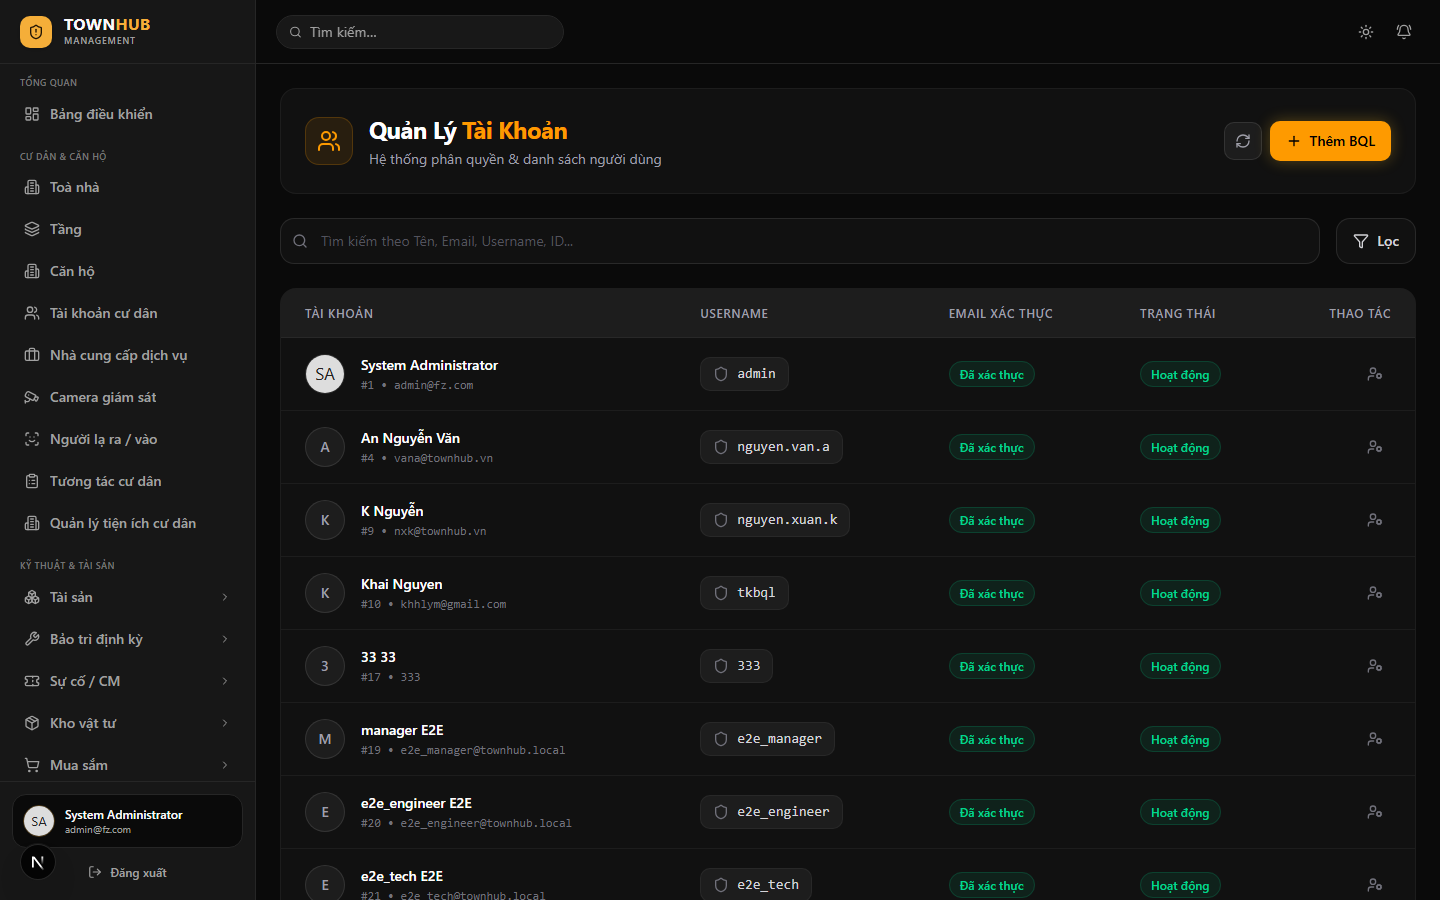
\includegraphics[width=\linewidth,height=0.82\textheight,keepaspectratio]{images/img42.png}
\caption*{\small Hình 5.1. Giao diện Quản trị Tài khoản người dùng}
\addcontentsline{lof}{figure}{Hình 5.1. Giao diện Quản trị Tài khoản người dùng}
\end{figure}
\begin{figure}[H]\centering
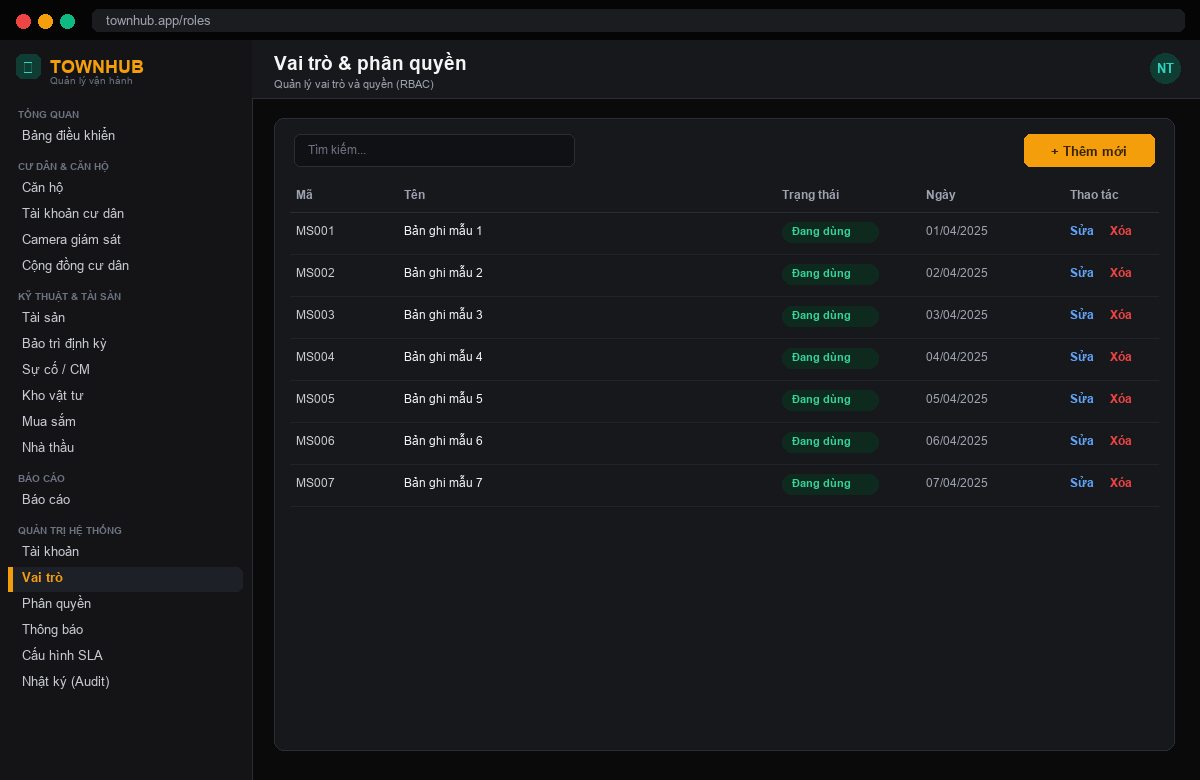
\includegraphics[width=\linewidth,height=0.82\textheight,keepaspectratio]{images/img43.png}
\caption*{\small Hình 5.2. Giao diện Vai trò \& phân quyền (RBAC)}
\addcontentsline{lof}{figure}{Hình 5.2. Giao diện Vai trò \& phân quyền (RBAC)}
\end{figure}
\phantomsection
\section*{5.3. Kết quả triển khai phân hệ Quản lý tài sản (phần riêng)}
\addcontentsline{toc}{section}{5.3. Kết quả triển khai phân hệ Quản lý tài sản (phần riêng)}
Phân hệ Quản lý tài sản do tác giả đảm nhiệm đã được hiện thực đầy đủ trên cả backend (API) và frontend (giao diện):

\begin{itemize}[leftmargin=1.4em,itemsep=1pt,topsep=2pt]
  \item \textbf{Tài sản \& bảo trì: }danh mục, ghi tăng, mã QR, điều chuyển, khấu hao, thanh lý; lịch bảo trì và Work Order (các route /assets*, /pm/*).
  \item \textbf{Kho – Mua sắm – Nhà cung cấp: }tồn kho \& cảnh báo tồn thấp, quy trình PR$\rightarrow$PO$\rightarrow$hóa đơn, OCR hóa đơn, quản lý NCC/hợp đồng (các route /inventory/*, /procurement/*, /vendors/*).
  \item \textbf{Sự cố \& SLA: }tạo và xử lý ticket, phân công, theo dõi SLA, leo thang, đánh giá hài lòng (các route /tickets/*, /my-tickets/*).
\end{itemize}
Giao diện thực tế của các phân hệ này đã được minh họa chi tiết ở Chương 4 (các Hình 4.6–4.8, 4.12–4.14 và 4.18–4.19). Toàn bộ chức năng đều hoạt động trên dữ liệu thật, có phân trang, tìm kiếm và phân quyền theo vai trò.

\phantomsection
\section*{5.4. Kiểm thử hệ thống}
\addcontentsline{toc}{section}{5.4. Kiểm thử hệ thống}
Hệ thống được kiểm thử theo phương pháp kiểm thử chức năng dựa trên ca kiểm thử, kết hợp thử nghiệm trực tiếp qua Swagger và giao diện; các thành viên trong nhóm kiểm thử chéo phân hệ của nhau để bảo đảm tính khách quan. Bảng dưới đây liệt kê một số ca kiểm thử tiêu biểu trải trên các phân hệ:

\begin{center}{\singlespacing\renewcommand{\arraystretch}{1.25}
\begin{tabular}{|>{\raggedright\arraybackslash}p{\dimexpr\linewidth/5-2\tabcolsep-\arrayrulewidth\relax}|>{\raggedright\arraybackslash}p{\dimexpr\linewidth/5-2\tabcolsep-\arrayrulewidth\relax}|>{\raggedright\arraybackslash}p{\dimexpr\linewidth/5-2\tabcolsep-\arrayrulewidth\relax}|>{\raggedright\arraybackslash}p{\dimexpr\linewidth/5-2\tabcolsep-\arrayrulewidth\relax}|>{\raggedright\arraybackslash}p{\dimexpr\linewidth/5-2\tabcolsep-\arrayrulewidth\relax}|}
\hline
\textbf{Mã} & \textbf{Chức năng} & \textbf{Dữ liệu vào} & \textbf{Kết quả mong đợi} & \textbf{KQ} \\ \hline
TC01 & Đăng nhập + MFA & email, mật khẩu, OTP & Nhận JWT, vào dashboard & Đạt \\ \hline
TC02 & Ghi tăng tài sản & mã, tên, danh mục, nguyên giá & Tạo tài sản + QR + chứng từ & Đạt \\ \hline
TC03 & Tính khấu hao kỳ & tài sản, kỳ & Ghi lich\_su\_khau\_hao & Đạt \\ \hline
TC04 & Cảnh báo tồn thấp & vật tư dưới ngưỡng & Xuất hiện ở get-low-stock & Đạt \\ \hline
TC05 & Duyệt PR $\rightarrow$ PO & PR hợp lệ & PR approved, tạo PO & Đạt \\ \hline
TC06 & OCR hóa đơn & ảnh hóa đơn & Trích xuất \& tạo Invoice & Đạt \\ \hline
TC07 & Ticket quá hạn SLA & ticket trễ hạn & Ghi SlaEscalationLog & Đạt \\ \hline
\end{tabular}}\end{center}
Toàn bộ ca kiểm thử và nhật ký lỗi được quản lý chi tiết trên tệp Excel dùng chung (mỗi lỗi kèm ảnh chụp, theo dõi qua 3 vòng test), minh họa ở Hình 5.3.

\begin{figure}[H]\centering
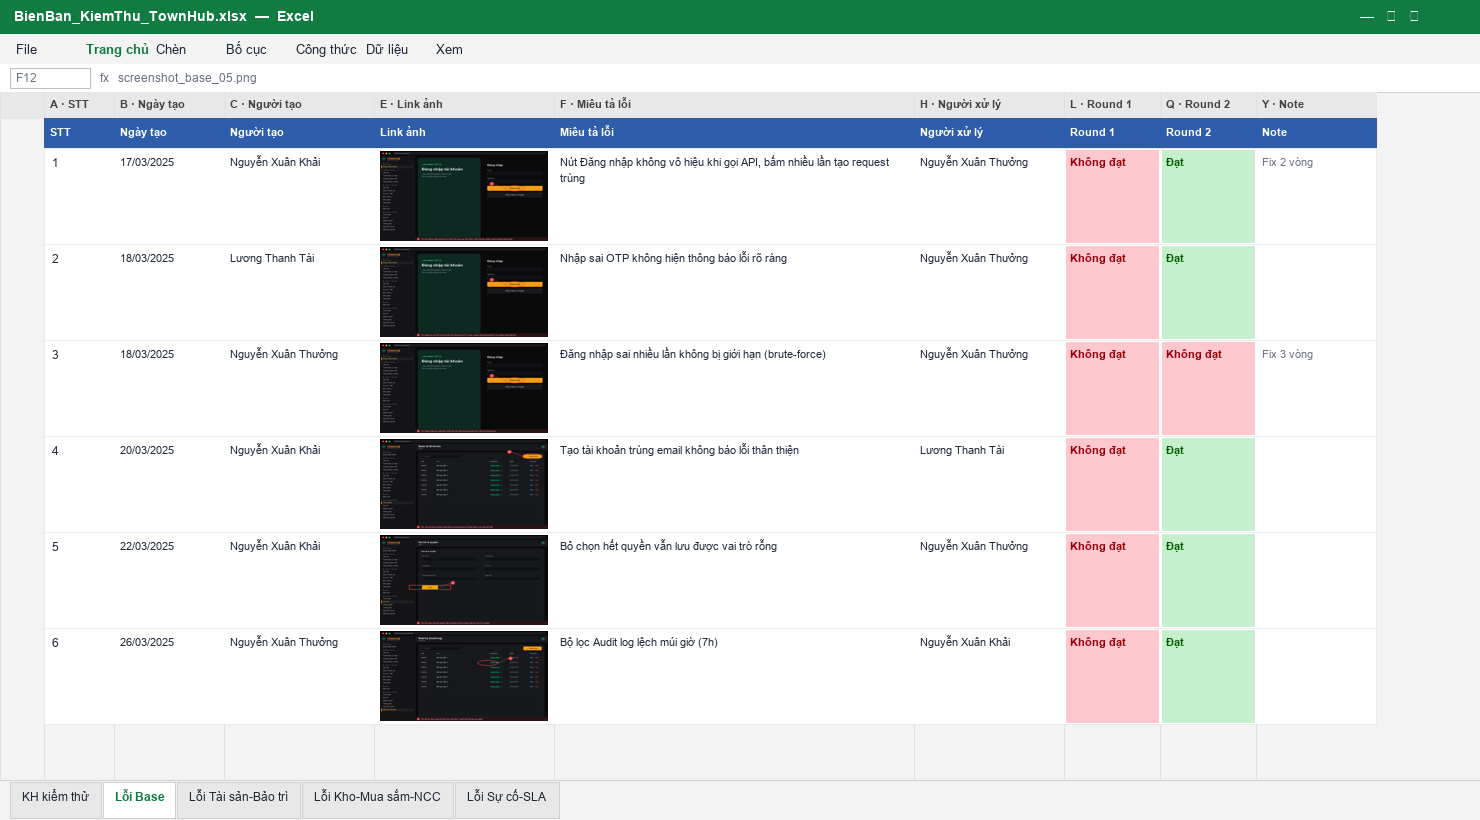
\includegraphics[width=\linewidth,height=0.82\textheight,keepaspectratio]{images/img44.png}
\caption*{\small Hình 5.3. Nhật ký lỗi \& kiểm thử trên Excel (sheet Lỗi Base)}
\addcontentsline{lof}{figure}{Hình 5.3. Nhật ký lỗi \& kiểm thử trên Excel (sheet Lỗi Base)}
\end{figure}
Kết quả kiểm thử cho thấy các chức năng chính hoạt động đúng yêu cầu. Các lỗi phát hiện trong quá trình phát triển đã được ghi nhận và khắc phục qua các vòng test.

\phantomsection
\section*{5.5. Đánh giá hệ thống}
\addcontentsline{toc}{section}{5.5. Đánh giá hệ thống}
Về mức độ đáp ứng yêu cầu, hệ thống đã hoàn thành các yêu cầu chức năng đặt ra ở Chương 1 cho cả phần Base và phân hệ Quản lý tài sản (phần riêng); kiến trúc module hóa giúp mã nguồn rõ ràng, dễ mở rộng và bảo trì. Về hiệu năng, các danh sách lớn được phân trang và lọc phía máy chủ; việc xử lý OCR bất đồng bộ qua hàng đợi giúp giao diện không bị chặn. Về bảo mật, hệ thống áp dụng JWT, MFA và phân quyền RBAC chi tiết. So với mục tiêu ban đầu, đề tài đạt được một sản phẩm chạy được, có giao diện và API hoàn chỉnh, tích hợp thành phần thông minh (OCR, khấu hao tự động).

\phantomsection
\section*{5.6. Đánh giá đạo đức, an toàn dữ liệu và bối cảnh xã hội}
\addcontentsline{toc}{section}{5.6. Đánh giá đạo đức, an toàn dữ liệu và bối cảnh xã hội}
Hệ thống xử lý dữ liệu cá nhân của cư dân và dữ liệu tài chính – kế toán của tòa nhà, do đó vấn đề đạo đức và an toàn dữ liệu được cân nhắc ngay trong thiết kế: áp dụng nguyên tắc phân quyền tối thiểu (chỉ vai trò phù hợp mới xem được dữ liệu nhạy cảm), lưu vết đầy đủ qua Audit Log, bảo vệ xác thực bằng MFA và mã hóa/không lưu mật khẩu dạng thô. Về bối cảnh kỹ thuật – xã hội, việc số hóa quản lý vận hành giúp minh bạch chi phí, giảm sai sót và nâng cao chất lượng dịch vụ cho cư dân; đồng thời hệ thống tôn trọng quyền riêng tư và tuân thủ quy định về sử dụng dữ liệu.

\phantomsection
\section*{5.7. Kết luận chương}
\addcontentsline{toc}{section}{5.7. Kết luận chương}
Chương 5 đã trình bày môi trường và kết quả triển khai, công tác kiểm thử cùng đánh giá tổng thể hệ thống trên các mặt chức năng, hiệu năng, bảo mật và đạo đức – an toàn dữ liệu. Kết quả cho thấy hệ thống TownHub đáp ứng tốt các mục tiêu đề ra.

\phantomsection
\chapter*{Kết luận}
\addcontentsline{toc}{chapter}{Kết luận}
\markboth{Kết luận}{Kết luận}
\phantomsection
\section*{1. Kết quả đạt được}
\addcontentsline{toc}{section}{1. Kết quả đạt được}
Đề tài đã xây dựng thành công hệ thống quản lý vận hành tòa nhà TownHub theo kiến trúc module hóa (.NET 8, Next.js 16, PostgreSQL). Phần Base do cả nhóm phối hợp xây dựng cung cấp đầy đủ dịch vụ nền tảng (xác thực – phân quyền, người dùng, thông báo, cấu hình, báo cáo). Về phần cá nhân, tác giả đã phân tích, thiết kế và hiện thực hoàn chỉnh phân hệ Quản lý tài sản, gồm các nghiệp vụ: Tài sản \& bảo trì (vòng đời tài sản, khấu hao đa phương pháp, mã QR, điều chuyển, bảo trì phòng ngừa, thanh lý, tích hợp kế toán); Kho – Mua sắm – Nhà cung cấp (tồn kho, quy trình PR$\rightarrow$PO$\rightarrow$hóa đơn, OCR hóa đơn bằng VietOCR, quản lý nhà cung cấp); và Quản lý sự cố \& SLA (quy trình xử lý khép kín, giám sát SLA và leo thang tự động). Hệ thống chạy được, có giao diện và API hoàn chỉnh, được kiểm thử và triển khai bằng Docker/Fly.io.

\phantomsection
\section*{2. Hạn chế}
\addcontentsline{toc}{section}{2. Hạn chế}
Bên cạnh kết quả đạt được, đề tài còn một số hạn chế: mô hình OCR hóa đơn cần thêm dữ liệu thực tế để nâng độ chính xác; một số báo cáo/thống kê nâng cao và tối ưu hiệu năng ở quy mô dữ liệu lớn chưa được kiểm chứng đầy đủ; ứng dụng di động cho cư dân/kỹ thuật viên mới ở mức cơ bản.

\phantomsection
\section*{3. Hướng phát triển}
\addcontentsline{toc}{section}{3. Hướng phát triển}
Trong tương lai, hệ thống có thể mở rộng theo các hướng: cải thiện độ chính xác OCR và bổ sung trích xuất thông minh hơn; tích hợp thiết bị IoT để giám sát tình trạng thiết bị theo thời gian thực và dự báo bảo trì; bổ sung phân tích dữ liệu và cảnh báo thông minh (dự báo hỏng hóc, tối ưu tồn kho); hoàn thiện ứng dụng di động và mở rộng các phân hệ khác của toàn hệ thống.

\phantomsection
\section*{4. Đóng góp của cá nhân}
\addcontentsline{toc}{section}{4. Đóng góp của cá nhân}
Trong khuôn khổ đồ án nhóm, tác giả (Nguyễn Xuân Thưởng) chịu trách nhiệm chính phân hệ Quản lý tài sản - gồm các nghiệp vụ Tài sản \& bảo trì, Kho – Mua sắm – Nhà cung cấp và Sự cố \& SLA (thuộc module Asset), đồng thời tham gia xây dựng phần Base dùng chung cùng cả nhóm. Toàn bộ phân tích, thiết kế, hiện thực và kiểm thử của phân hệ nêu trên do tác giả trực tiếp thực hiện; đồng thời tác giả phối hợp với các thành viên khác trong việc thống nhất quy ước API, liên thông dữ liệu với hai phân hệ Quản lý dân cư và Quản lý dịch vụ, và review chéo khi hợp nhất mã nguồn. Sự phân định phần chung – phần riêng này thể hiện rõ đóng góp cá nhân theo Điều 7 Quy định ĐATN.

\phantomsection
\chapter*{Tài liệu tham khảo}
\addcontentsline{toc}{chapter}{Tài liệu tham khảo}
\markboth{Tài liệu tham khảo}{Tài liệu tham khảo}
\textit{$\rightarrow$ Trích dẫn chuẩn IEEE/APA, đánh số [1], [2]\ldots{} khớp với chỗ trích trong bài.}

\begin{itemize}[leftmargin=1.4em,itemsep=1pt,topsep=2pt]
  \item Microsoft, ``ASP.NET Core documentation'', learn.microsoft.com.
  \item Vercel, ``Next.js Documentation'', nextjs.org/docs.
  \item S-TECH, ``Phần mềm quản lý tòa nhà Building Care'', \url{https://buildingcare.biz/}.
  \item S-TECH, ``FLC Twin Towers 265 Cầu Giấy chính thức triển khai phần mềm Building Care'', 27/06/2025, \url{https://s-tech.info/flc-twin-towers-265-cau-giay-chinh-thuc-trien-khai-phan-mem-building-care/}.
  \item Landsoft, ``Landsoft Control và hành trình 6 năm đồng hành cùng Xuân Mai Corp'', \url{https://landsoft.com.vn/landsoft-control-va-hanh-trinh-6-nam-dong-hanh-cung-xuan-mai-corp-xay-dung-thuong-hieu-quan-ly-van-hanh-chuyen-nghiep/}.
  \item DIP Holding, ``GELEXIMCO số hóa bộ máy quản lý chuỗi tòa nhà bằng phần mềm Landsoft Control'', 25/02/2021, \url{https://dip.vn/geleximco-so-hoa-bo-may-quan-ly-chuoi-toa-nha-chuyen-nghiep-hon-bang-phan-mem-landsoft-control/}.
  \item Báo Tuổi Trẻ, ``Ứng dụng giải bài toán hết cảnh xếp hàng đóng phí chung cư'', 01/05/2023, \url{https://tuoitre.vn/ung-dung-giai-bai-toan-het-canh-xep-hang-dong-phi-chung-cu-20230425232909509.htm}.
  \item CYFEER, ``CyHome PMS'' (ứng dụng cho kỹ thuật viên), Google Play, \url{https://play.google.com/store/apps/details?id=com.cyfeer.cyhome_manager&hl=vi}.
\end{itemize}
\phantomsection
\chapter*{Phụ lục}
\addcontentsline{toc}{chapter}{Phụ lục}
\markboth{Phụ lục}{Phụ lục}
\textit{$\rightarrow$ Nhật ký thực hiện ĐATN (Mẫu ĐATN-02); bảng phân công chi tiết; đặc tả API đầy đủ (Swagger); sơ đồ CSDL tổng thể (schema auth/asset/base); hướng dẫn cài đặt \& sử dụng.}

\textbf{Phụ lục. Nhật ký thực hiện ĐATN (Mẫu ĐATN-02)}

\textit{Mẫu ĐATN-02}

\begin{center}{\singlespacing\renewcommand{\arraystretch}{1.25}
\begin{tabular}{|>{\raggedright\arraybackslash}p{\dimexpr\linewidth/2-2\tabcolsep-\arrayrulewidth\relax}|>{\raggedright\arraybackslash}p{\dimexpr\linewidth/2-2\tabcolsep-\arrayrulewidth\relax}|}
\hline
\textbf{TRƯỜNG ĐẠI HỌC XÂY DỰNG HÀ NỘI} \newline \textbf{KHOA CÔNG NGHỆ THÔNG TIN} & \textbf{CỘNG HOÀ XÃ HỘI CHỦ NGHĨA VIỆT NAM} \newline \textbf{Độc lập - Tự do - Hạnh phúc} \\ \hline
\end{tabular}}\end{center}
\textbf{Nhật ký thực hiện ĐATN}

\textit{(Ban hành kèm theo Quyết định số     /QĐ-ĐHXDHN ngày     tháng     năm 2026 của Hiệu trưởng Trường Đại học Xây dựng Hà Nội)}

\begin{center}{\singlespacing\renewcommand{\arraystretch}{1.25}
\begin{tabular}{|>{\raggedright\arraybackslash}p{\dimexpr\linewidth/2-2\tabcolsep-\arrayrulewidth\relax}|>{\raggedright\arraybackslash}p{\dimexpr\linewidth/2-2\tabcolsep-\arrayrulewidth\relax}|}
\hline
\textbf{Họ và tên SV} & Nguyễn Xuân Thưởng \\ \hline
\textbf{Mã SV} & 0220766 \\ \hline
\textbf{Tên đề tài} & Xây dựng hệ thống quản lý vận hành tòa nhà – TownHub \\ \hline
\textbf{Đợt} & 2026 \\ \hline
\textbf{GVHD} & ThS. Hoàng Nam Thắng \\ \hline
\textbf{Đơn vị} & Khoa Công nghệ thông tin \\ \hline
\textbf{GV đồng hướng dẫn (nếu có)} & (không có) \\ \hline
\end{tabular}}\end{center}
\begin{landscape}{\footnotesize\singlespacing\renewcommand{\arraystretch}{1.25}\setlength{\LTleft}{0pt}\setlength{\LTright}{0pt}
\begin{longtable}{|>{\raggedright\arraybackslash}p{\dimexpr\linewidth/8-2\tabcolsep-\arrayrulewidth\relax}|>{\raggedright\arraybackslash}p{\dimexpr\linewidth/8-2\tabcolsep-\arrayrulewidth\relax}|>{\raggedright\arraybackslash}p{\dimexpr\linewidth/8-2\tabcolsep-\arrayrulewidth\relax}|>{\raggedright\arraybackslash}p{\dimexpr\linewidth/8-2\tabcolsep-\arrayrulewidth\relax}|>{\raggedright\arraybackslash}p{\dimexpr\linewidth/8-2\tabcolsep-\arrayrulewidth\relax}|>{\raggedright\arraybackslash}p{\dimexpr\linewidth/8-2\tabcolsep-\arrayrulewidth\relax}|>{\raggedright\arraybackslash}p{\dimexpr\linewidth/8-2\tabcolsep-\arrayrulewidth\relax}|>{\raggedright\arraybackslash}p{\dimexpr\linewidth/8-2\tabcolsep-\arrayrulewidth\relax}|}
\hline
\textbf{Loại công việc} & \textbf{Thời gian làm việc} & \textbf{Nhiệm vụ được giao} & \textbf{Kết quả thực hiện} & \textbf{Kiến thức/​kỹ năng áp dụng} & \textbf{Vấn đề cần bổ sung, chỉnh sửa} & \textbf{Tự đánh giá \& rút kinh nghiệm} & \textbf{Chữ ký} \\ \hline
\endhead
\textbf{Tuần 1:  \ldots{}\ldots{}/\ldots{}\ldots{}  -  \ldots{}\ldots{}/\ldots{}\ldots{}} &  &  &  &  &  &  &  \\ \hline
Làm việc độc lập & \textasciitilde{}12 giờ & Đọc chương 1 học phần ĐATN; tìm hiểu bài toán quản lý vận hành tòa nhà; khảo sát yêu cầu các phân hệ Tài sản, Kho–Mua sắm, Sự cố. & Hoàn thành khảo sát và đặc tả yêu cầu; phác thảo kiến trúc phân hệ phụ trách. & Phân tích yêu cầu; kiến trúc phần mềm; .NET 8, Next.​js. & Chuẩn hóa lại phạm vi từng phân hệ. & Cần bám sát chuẩn đầu ra học phần. & SV / GVHD \\ \hline
Làm việc theo nhóm & \textasciitilde{}8 giờ & Thống nhất kiến trúc tổng thể; phân chia module Base và phần riêng; thiết lập Git, quy ước code. & Khung dự án chạy được; phân công công việc rõ ràng. & Làm việc nhóm; Git; quản lý dự án. & Thống nhất chuẩn code và CSDL chung. & Cần phối hợp chặt chẽ hơn. & SV / GVHD \\ \hline
\textbf{Tuần 2:  \ldots{}\ldots{}/\ldots{}\ldots{}  -  \ldots{}\ldots{}/\ldots{}\ldots{}} &  &  &  &  &  &  &  \\ \hline
Làm việc độc lập & \textasciitilde{}14 giờ & Thiết kế CSDL schema asset (ERD); thiết kế API và phân quyền cho phân hệ Tài sản. & Hoàn thành ERD và bộ API tài sản; sinh sơ đồ bằng draw.​io. & Thiết kế CSDL quan hệ; REST API; RBAC. & Rà soát ràng buộc khóa ngoại. & Cần đặt tên nhất quán. & SV / GVHD \\ \hline
\textbf{Tuần 3:  \ldots{}\ldots{}/\ldots{}\ldots{}  -  \ldots{}\ldots{}/\ldots{}\ldots{}} &  &  &  &  &  &  &  \\ \hline
Làm việc độc lập & \textasciitilde{}14 giờ & Cài đặt vòng đời tài sản: ghi tăng, điều chuyển, thanh lý; khấu hao tự động; sinh \& in mã QR. & Các chức năng tài sản chạy được; khấu hao định kỳ tự động. & EF Core; job nền; sinh mã QR. & Kiểm thử các phương pháp khấu hao. & Cần thêm ràng buộc nghiệp vụ. & SV / GVHD \\ \hline
\textbf{Tuần 4:  \ldots{}\ldots{}/\ldots{}\ldots{}  -  \ldots{}\ldots{}/\ldots{}\ldots{}} &  &  &  &  &  &  &  \\ \hline
Làm việc độc lập & \textasciitilde{}14 giờ & Cài đặt bảo trì phòng ngừa (PM): lịch bảo trì, lệnh công việc (WO), checklist, nghiệm thu. & Quy trình PM và Work Order hoạt động; đính kèm ảnh minh chứng. & Máy trạng thái; hàng đợi; lịch cron. & Chuẩn hóa trạng thái WO. & Cần tối ưu truy vấn danh sách. & SV / GVHD \\ \hline
\textbf{Tuần 5:  \ldots{}\ldots{}/\ldots{}\ldots{}  -  \ldots{}\ldots{}/\ldots{}\ldots{}} &  &  &  &  &  &  &  \\ \hline
Làm việc độc lập & \textasciitilde{}14 giờ & Cài đặt Kho – Mua sắm – NCC: tồn kho, cảnh báo tồn thấp, quy trình PR $\rightarrow$ PO, quản lý NCC/​hợp đồng. & Quy trình mua sắm nhiều cấp chạy được; cảnh báo tồn kho. & Thiết kế quy trình duyệt; giao dịch CSDL. & Rà soát luồng duyệt nhiều cấp. & Cần bổ sung nhật ký thao tác. & SV / GVHD \\ \hline
\textbf{Tuần 6:  \ldots{}\ldots{}/\ldots{}\ldots{}  -  \ldots{}\ldots{}/\ldots{}\ldots{}} &  &  &  &  &  &  &  \\ \hline
Làm việc độc lập & \textasciitilde{}14 giờ & Tích hợp OCR hóa đơn: sinh dataset hóa đơn tổng hợp; huấn luyện \& đánh giá VietOCR, PaddleOCR; nối dịch vụ OCR với backend. & Dịch vụ OCR chạy; PaddleOCR val-acc 99,64\%; có bảng so sánh 3 engine. & AI/​OCR; PyTorch/​Paddle; FastAPI; hàng đợi nền. & Cần thêm hóa đơn thật để cải thiện phát hiện. & Đánh giá khách quan giữa các engine. & SV / GVHD \\ \hline
\textbf{Tuần 7:  \ldots{}\ldots{}/\ldots{}\ldots{}  -  \ldots{}\ldots{}/\ldots{}\ldots{}} &  &  &  &  &  &  &  \\ \hline
Làm việc độc lập & \textasciitilde{}14 giờ & Cài đặt Quản lý sự cố \& SLA: tạo ticket, phân công KTV, giám sát và leo thang SLA, dashboard. & Phân hệ sự cố hoạt động; theo dõi SLA thời gian thực. & Sự kiện/​thông báo; đo lường SLA; realtime. & Chuẩn hóa mức ưu tiên và SLA. & Cần bổ sung báo cáo thống kê. & SV / GVHD \\ \hline
\textbf{Tuần 8:  \ldots{}\ldots{}/\ldots{}\ldots{}  -  \ldots{}\ldots{}/\ldots{}\ldots{}} &  &  &  &  &  &  &  \\ \hline
Làm việc độc lập & \textasciitilde{}14 giờ & Kiểm thử và tích hợp toàn hệ thống; sửa lỗi; viết thuyết minh ĐATN; dựng sơ đồ (draw.​io); chuẩn bị bảo vệ. & Hệ thống chạy ổn định; hoàn thành quyển thuyết minh và biên bản kiểm thử. & Kiểm thử; viết tài liệu; trình bày. & Hoàn thiện định dạng theo mẫu ĐATN. & Cần luyện trình bày bảo vệ. & SV / GVHD \\ \hline
\end{longtable}}\end{landscape}
\textit{Ghi chú: sinh viên điền mốc thời gian từng tuần và ký xác nhận cùng GVHD.}

% ======================================================================
%  PHỤ LỤC: BIÊN BẢN KIỂM THỬ HỆ THỐNG THEO VAI TRÒ
%  (sinh tự động từ bộ kiểm thử E2E Playwright chạy trên hệ thống thật)
% ======================================================================
\clearpage
\phantomsection
\addcontentsline{toc}{section}{Phụ lục. Biên bản kiểm thử hệ thống theo vai trò}
\markboth{Phụ lục — Kiểm thử}{Phụ lục — Kiểm thử}

\begin{center}\textbf{\large PHỤ LỤC. BIÊN BẢN KIỂM THỬ HỆ THỐNG THEO VAI TRÒ}\end{center}
\smallskip

Toàn bộ kịch bản kiểm thử dưới đây được \textbf{tự động hoá} bằng Playwright và thực thi \textbf{trực tiếp trên hệ thống đang chạy} (không dùng dữ liệu giả lập), bao trùm bốn luồng nghiệp vụ chính của TownHub. Điểm cốt lõi: kịch bản được xây dựng \textit{theo vai trò} — mỗi vai trò đăng nhập bằng tài khoản riêng và chỉ thực hiện đúng phần việc được phân quyền trong quy trình, thay vì để một tài khoản quản trị làm toàn bộ. Nhờ đó biên bản đồng thời kiểm chứng được cả nghiệp vụ (happy case) lẫn cơ chế kiểm soát truy cập/tách bạch nhiệm vụ (side case — kỳ vọng bị chặn \texttt{403}).

\textbf{Môi trường kiểm thử:}
\begin{itemize}[leftmargin=1.5em,itemsep=1pt,topsep=2pt]
  \item \textbf{Backend:} ASP.NET Core .NET 8, chạy tại \texttt{localhost:5267}; CSDL PostgreSQL (Neon).
  \item \textbf{Frontend:} Next.js 16 (React 19), chạy tại \texttt{localhost:3000}.
  \item \textbf{Dịch vụ OCR:} worker nền xử lý hàng đợi; ở môi trường kiểm thử dùng engine mô phỏng nên job OCR chạy đến trạng thái \texttt{COMPLETED} (mô hình OCR thực tế được đánh giá riêng ở Chương~2).
  \item \textbf{Công cụ:} Playwright (trình duyệt Chromium), chạy tuần tự một luồng để không quá tải CSDL đám mây.
  \item \textbf{Tài khoản:} 6 tài khoản ứng với 6 vai trò RBAC (Quản trị viên, Ban quản lý, Kỹ sư trưởng, Kỹ thuật viên, Kế toán, Cư dân).
\end{itemize}

\textbf{Kết quả tổng hợp:} \textbf{40/40} ca kiểm thử chức năng \textbf{ĐẠT} (20 ca thao tác hợp lệ + 20 ca kiểm soát/từ chối truy cập \texttt{403}), kèm 19 lượt chụp màn hình minh hoạ giao diện theo vai trò. Chi tiết ở các bảng và hình bên dưới.

\medskip
\textbf{Bảng PL.1. Tổng hợp kết quả theo nhóm chức năng}

\begin{center}{\small\renewcommand{\arraystretch}{1.2}
\begin{tabular}{|>{\raggedright\arraybackslash}p{0.40\linewidth}|c|c|c|}
\hline
\rowcolor{gray!15}\textbf{Nhóm chức năng} & \textbf{Happy} & \textbf{Side} & \textbf{Đạt} \\ \hline
Xác thực \& Phân quyền (Auth/RBAC) & 6 & 5 & 11/11 \\ \hline
Luồng Sự cố (Cư dân → BQL → KTV) & 3 & 4 & 7/7 \\ \hline
Luồng Mua sắm \& OCR (KST → BQL → Kế toán) & 4 & 4 & 8/8 \\ \hline
Luồng Tài sản (KST tạo · Kế toán vận hành) & 4 & 4 & 8/8 \\ \hline
Luồng Bảo trì / Work Order (BQL giao · KTV thực thi) & 3 & 3 & 6/6 \\ \hline
\rowcolor{gray!15}\textbf{Tổng} & \textbf{20} & \textbf{20} & \textbf{40/40} \\ \hline
\end{tabular}}\end{center}

\medskip
\textbf{Bảng PL.2. Ma trận phân quyền theo vai trò (kiểm chứng bằng kiểm thử)}

\noindent Ký hiệu: \checkmark{} = được phép (kiểm thử happy \texttt{200}); $\times$ = bị chặn (kiểm thử side \texttt{403}). Viết tắt vai trò: QTV = Quản trị viên, BQL = Ban quản lý, KST = Kỹ sư trưởng, KTV = Kỹ thuật viên, KT = Kế toán, CD = Cư dân.

\begin{center}{\small\renewcommand{\arraystretch}{1.25}
\begin{tabular}{|>{\raggedright\arraybackslash}p{0.34\linewidth}|c|c|c|c|c|c|}
\hline
\rowcolor{gray!15}\textbf{Hành động nghiệp vụ} & \textbf{QTV} & \textbf{BQL} & \textbf{KST} & \textbf{KTV} & \textbf{KT} & \textbf{CD} \\ \hline
Đăng nhập hệ thống & \checkmark & \checkmark & \checkmark & \checkmark & \checkmark & \checkmark \\ \hline
Xem danh sách tài sản & \checkmark & \checkmark & \checkmark & \checkmark & \checkmark & $\times$ \\ \hline
Tạo mới tài sản & \checkmark & $\times$ & \checkmark & $\times$ & $\times$ & $\times$ \\ \hline
Cập nhật / khấu hao tài sản & \checkmark & \checkmark & \checkmark & $\times$ & \checkmark & $\times$ \\ \hline
Tạo ticket sự cố & \checkmark & $\times$ & \checkmark & $\times$ & $\times$ & \checkmark \\ \hline
Phân công ticket cho KTV & \checkmark & \checkmark & \checkmark & $\times$ & $\times$ & $\times$ \\ \hline
Xử lý (chuyển trạng thái) ticket & \checkmark & $\times$ & \checkmark & \checkmark & $\times$ & $\times$ \\ \hline
Tạo phiếu yêu cầu mua sắm (PR) & \checkmark & \checkmark & \checkmark & $\times$ & $\times$ & $\times$ \\ \hline
Duyệt phiếu yêu cầu mua sắm & \checkmark & \checkmark & $\times$ & $\times$ & $\times$ & $\times$ \\ \hline
Xử lý OCR hoá đơn & \checkmark & $\times$ & $\times$ & $\times$ & \checkmark & $\times$ \\ \hline
Tạo lệnh công việc (Work Order) & \checkmark & \checkmark & \checkmark & $\times$ & $\times$ & $\times$ \\ \hline
Thực thi Work Order (đính minh chứng) & \checkmark & $\times$ & \checkmark & \checkmark & $\times$ & $\times$ \\ \hline
\end{tabular}}\end{center}

\smallskip
\noindent\textit{Nhận xét: ma trận thể hiện rõ nguyên tắc tách bạch nhiệm vụ — người đề xuất mua sắm (Kỹ sư trưởng) không được tự duyệt; Ban quản lý điều phối/giao việc nhưng không trực tiếp thực thi kỹ thuật; Kế toán phụ trách hoá đơn nhưng không được duyệt phiếu yêu cầu; Cư dân chỉ báo sự cố và tra cứu.}

% --------------------------------------------------------------
%  BẢNG CHI TIẾT TEST CASE (trang ngang)
% --------------------------------------------------------------
\begin{landscape}{\footnotesize\singlespacing\renewcommand{\arraystretch}{1.25}\setlength{\LTleft}{0pt}\setlength{\LTright}{0pt}
\textbf{Bảng PL.3. Chi tiết ca kiểm thử theo vai trò và kết quả thực tế}\par\smallskip
\begin{longtable}{|>{\raggedright\arraybackslash}p{0.07\linewidth}|>{\raggedright\arraybackslash}p{0.11\linewidth}|>{\raggedright\arraybackslash}p{0.30\linewidth}|>{\raggedright\arraybackslash}p{0.27\linewidth}|>{\raggedright\arraybackslash}p{0.13\linewidth}|c|}
\hline
\rowcolor{gray!20}\textbf{Mã} & \textbf{Vai trò} & \textbf{Kịch bản / thao tác} & \textbf{Kết quả mong đợi} & \textbf{Thực tế} & \textbf{KQ} \\ \hline
\endhead

\multicolumn{6}{|l|}{\cellcolor{blue!8}\textbf{A. Xác thực \& Phân quyền (Auth/RBAC)}} \\ \hline
TC-AUTH-01 & (mọi) & Đăng nhập với thông tin hợp lệ trên giao diện & Vào được dashboard, hiện menu theo quyền & Vào dashboard & \checkmark \\ \hline
TC-AUTH-03 & (mọi) & Đăng nhập sai mật khẩu & Báo lỗi, ở lại trang đăng nhập & Báo lỗi & \checkmark \\ \hline
TC-AUTH-04 & (mọi) & Bỏ trống tài khoản/mật khẩu & Chặn phía client, nhắc nhập & Bị chặn & \checkmark \\ \hline
TC-AUTH-05 & (mọi) & Đăng nhập qua API & Trả token JWT kèm danh sách quyền & Có token+quyền & \checkmark \\ \hline
TC-AUTH-06 & (mọi) & Đăng nhập API sai mật khẩu & Không trả token & Không token & \checkmark \\ \hline
TC-AUTH-07 & — & Gọi API bảo vệ khi chưa đăng nhập & Bị từ chối \texttt{401 Unauthorized} & \texttt{401} & \checkmark \\ \hline
TC-RBAC-a & Ban quản lý & Quyền trong JWT đúng thiết kế (có duyệt PR/phân công; không tạo ticket, không thực thi WO) & Khớp ma trận PL.2 & Khớp & \checkmark \\ \hline
TC-RBAC-b & Kỹ sư trưởng & Có tạo tài sản/ticket/WO, đề xuất PR; không duyệt PR, không OCR & Khớp ma trận PL.2 & Khớp & \checkmark \\ \hline
TC-RBAC-c & Kỹ thuật viên & Có xem tài sản, xử lý ticket, thực thi WO; không tạo ticket/WO/tài sản & Khớp ma trận PL.2 & Khớp & \checkmark \\ \hline
TC-RBAC-d & Kế toán & Có OCR/hoá đơn, cập nhật tài sản, báo cáo; không tạo tài sản, không duyệt PR & Khớp ma trận PL.2 & Khớp & \checkmark \\ \hline
TC-RBAC-e & Cư dân & Chỉ có tạo/xem ticket, xem thông báo; không xem tài sản, không duyệt & Khớp ma trận PL.2 & Khớp & \checkmark \\ \hline

\multicolumn{6}{|l|}{\cellcolor{blue!8}\textbf{B. Luồng Sự cố: Cư dân → Ban quản lý → Kỹ thuật viên}} \\ \hline
TC-INC-10 & Cư dân & Tạo ticket báo sự cố (mất điện hành lang) & Tạo thành công, sinh mã \texttt{TK-*} & Mã \texttt{TK-*} & \checkmark \\ \hline
TC-INC-11 & Cư dân & Thử xem danh sách tài sản & Bị chặn \texttt{403} & \texttt{403} & \checkmark \\ \hline
TC-INC-12 & Kỹ thuật viên & Thử tạo ticket & Bị chặn \texttt{403} (KTV không có quyền tạo) & \texttt{403} & \checkmark \\ \hline
TC-INC-13 & Ban quản lý & Phân công KTV xử lý ticket & Phân công thành công \texttt{200} & \texttt{200} & \checkmark \\ \hline
TC-INC-14 & Ban quản lý & Thử tự chuyển trạng thái (resolve) ticket & Bị chặn \texttt{403} (không có quyền xử lý) & \texttt{403} & \checkmark \\ \hline
TC-INC-15 & Kỹ thuật viên & Chuyển ticket sang trạng thái đang xử lý & Cập nhật thành công \texttt{200} & \texttt{200} & \checkmark \\ \hline
TC-INC-16 & Cư dân & Thử phân công ticket & Bị chặn \texttt{403} & \texttt{403} & \checkmark \\ \hline

\multicolumn{6}{|l|}{\cellcolor{blue!8}\textbf{C. Luồng Mua sắm \& OCR: Kỹ sư trưởng → Ban quản lý → Kế toán}} \\ \hline
TC-PRO-10 & Kỹ sư trưởng & Tạo và gửi duyệt phiếu yêu cầu (PR) & Tạo được, sinh mã \texttt{PR-*}, gửi duyệt & Mã \texttt{PR-*} & \checkmark \\ \hline
TC-PRO-11 & Kỹ sư trưởng & Thử tự duyệt PR do mình đề xuất & Bị chặn \texttt{403} (tách bạch nhiệm vụ) & \texttt{403} & \checkmark \\ \hline
TC-PRO-12 & Ban quản lý & Duyệt PR do Kỹ sư trưởng gửi & Duyệt thành công \texttt{200} & \texttt{200} & \checkmark \\ \hline
TC-PRO-13 & Kế toán & Thử duyệt PR & Bị chặn \texttt{403} & \texttt{403} & \checkmark \\ \hline
TC-PRO-14 & Cư dân & Thử tạo PR & Bị chặn \texttt{403} & \texttt{403} & \checkmark \\ \hline
TC-OCR-15 & Kế toán & Gửi hoá đơn cho OCR & Job được xử lý đến trạng thái kết thúc & \texttt{COMPLETED} & \checkmark \\ \hline
TC-OCR-16 & Ban quản lý & Thử gửi OCR hoá đơn & Bị chặn \texttt{403} (không có quyền hoá đơn) & \texttt{403} & \checkmark \\ \hline
TC-PRO-x & (kết hợp) & Chuỗi PR: đề xuất → gửi → duyệt hoàn tất & Vòng đời PR chạy đúng qua 2 vai trò & Đúng & \checkmark \\ \hline

\multicolumn{6}{|l|}{\cellcolor{blue!8}\textbf{D. Luồng Quản lý tài sản: Kỹ sư trưởng tạo · Kế toán vận hành}} \\ \hline
TC-AST-10 & Kỹ sư trưởng & Tạo mới tài sản (kèm nguyên giá, khấu hao) & Tạo thành công \texttt{200} & \texttt{200} & \checkmark \\ \hline
TC-AST-11 & Kỹ thuật viên & Thử tạo tài sản & Bị chặn \texttt{403} & \texttt{403} & \checkmark \\ \hline
TC-AST-12 & Kế toán & Thử tạo tài sản & Bị chặn \texttt{403} (chỉ được cập nhật) & \texttt{403} & \checkmark \\ \hline
TC-AST-13 & Kế toán & Xem tài sản + báo cáo bảng cân đối thử & Truy cập thành công \texttt{200} & \texttt{200} & \checkmark \\ \hline
TC-AST-14 & Kế toán & Cập nhật tài sản (kiểm tra phân quyền) & Được phép (không bị \texttt{403}) & Không \texttt{403} & \checkmark \\ \hline
TC-AST-15 & Kỹ thuật viên & Thử cập nhật tài sản & Bị chặn \texttt{403} & \texttt{403} & \checkmark \\ \hline
TC-AST-16 & Kỹ thuật viên & Xem danh sách tài sản & Truy cập thành công \texttt{200} & \texttt{200} & \checkmark \\ \hline
TC-AST-17 & Cư dân & Thử xem danh sách tài sản & Bị chặn \texttt{403} & \texttt{403} & \checkmark \\ \hline

\multicolumn{6}{|l|}{\cellcolor{blue!8}\textbf{E. Luồng Bảo trì / Work Order: Ban quản lý giao · Kỹ thuật viên thực thi}} \\ \hline
TC-WO-10 & Ban quản lý & Tạo lệnh công việc (Work Order) & Tạo được, sinh mã \texttt{WO-*} & Mã \texttt{WO} & \checkmark \\ \hline
TC-WO-11 & Ban quản lý & Phân công KTV cho Work Order & Phân công thành công \texttt{200} & \texttt{200} & \checkmark \\ \hline
TC-WO-12 & Ban quản lý & Thử tự thực thi WO (đính minh chứng) & Bị chặn \texttt{403} (chỉ giao, không thực thi) & \texttt{403} & \checkmark \\ \hline
TC-WO-13 & Kỹ thuật viên & Thử tạo Work Order & Bị chặn \texttt{403} & \texttt{403} & \checkmark \\ \hline
TC-WO-14 & Kỹ thuật viên & Thực thi WO: đính kèm ảnh minh chứng & Thực thi thành công \texttt{200} & \texttt{200} & \checkmark \\ \hline
TC-WO-15 & Kế toán & Thử xem danh sách Work Order & Bị chặn \texttt{403} & \texttt{403} & \checkmark \\ \hline
\end{longtable}}\end{landscape}

% --------------------------------------------------------------
%  ẢNH MINH HOẠ
% --------------------------------------------------------------
\clearpage
\textbf{Ảnh minh hoạ 1 — Dashboard hiển thị theo vai trò (menu chức năng thay đổi theo quyền).}

\begin{figure}[H]\centering
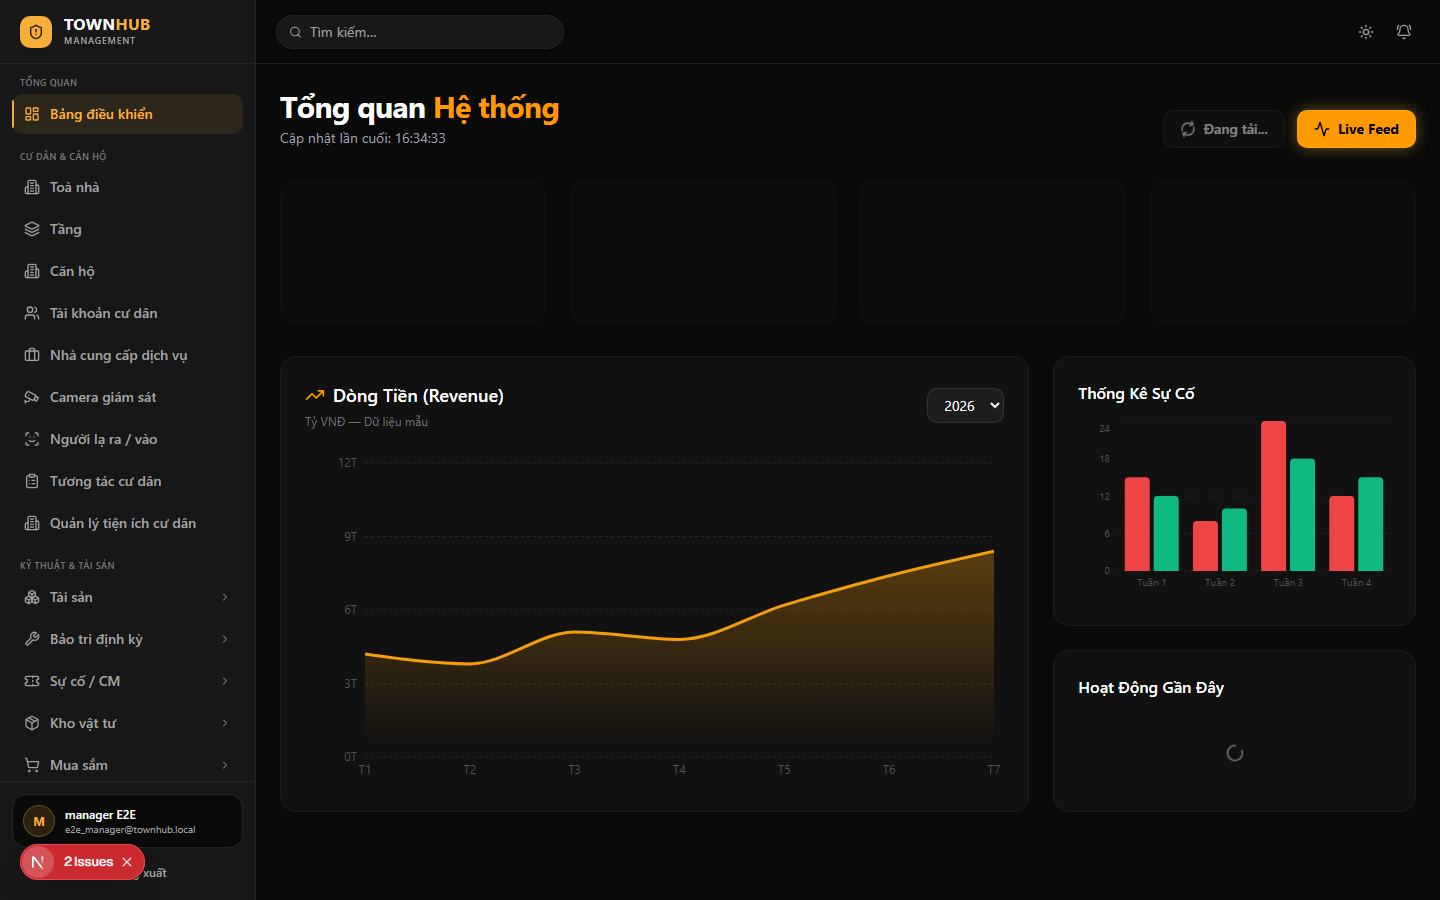
\includegraphics[width=\linewidth,height=0.44\textheight,keepaspectratio]{images/tc_role_manager_dashboard.png}
\caption*{\small Hình PL.1. Giao diện đăng nhập vai trò \textbf{Ban quản lý}.}
\end{figure}
\begin{figure}[H]\centering
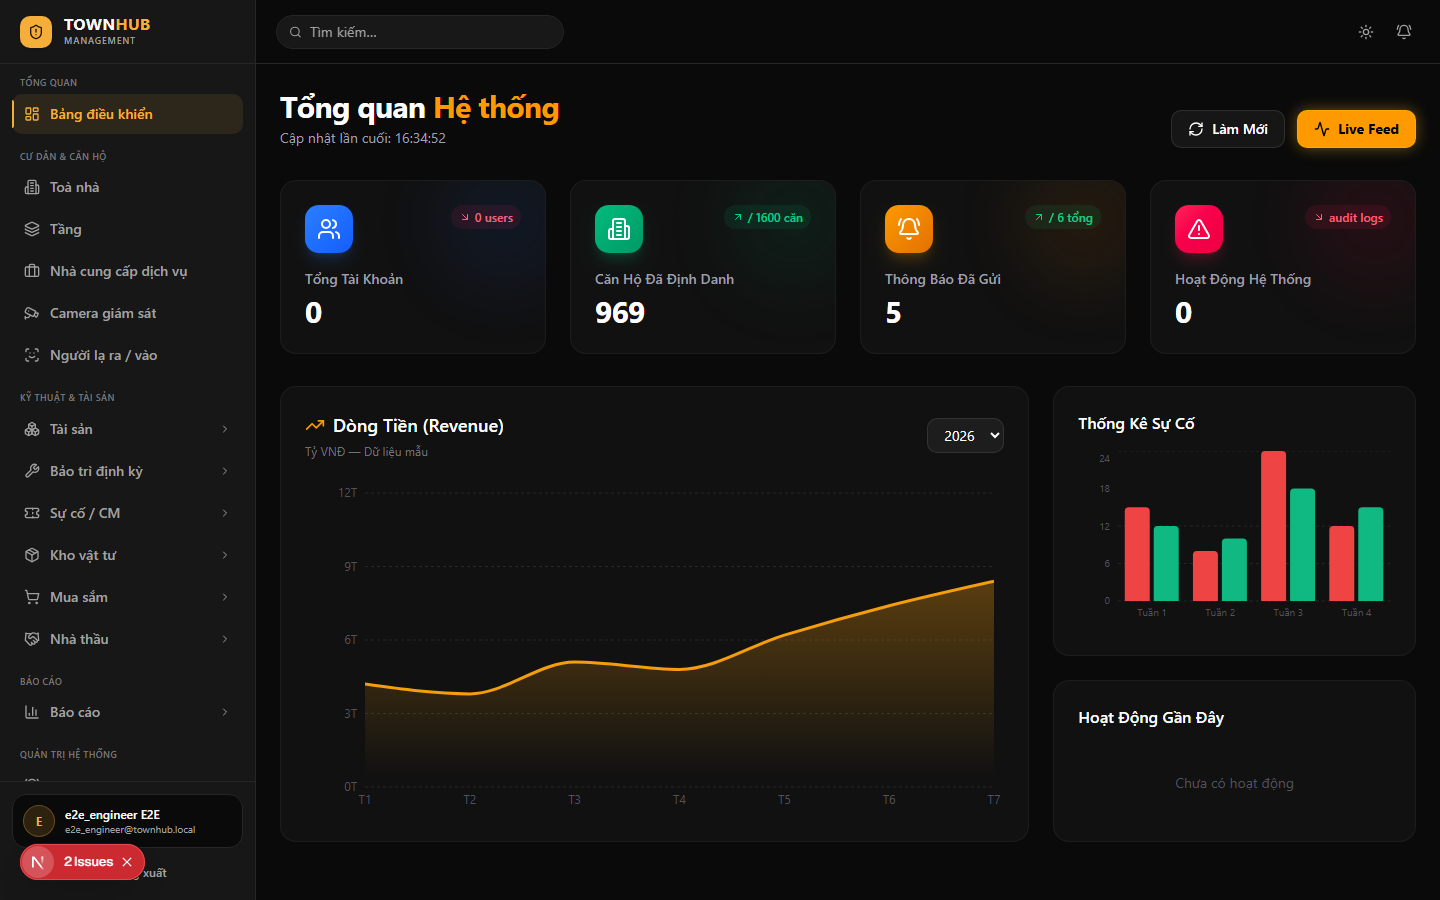
\includegraphics[width=\linewidth,height=0.44\textheight,keepaspectratio]{images/tc_role_engineer_dashboard.png}
\caption*{\small Hình PL.2. Giao diện đăng nhập vai trò \textbf{Kỹ sư trưởng}.}
\end{figure}
\begin{figure}[H]\centering
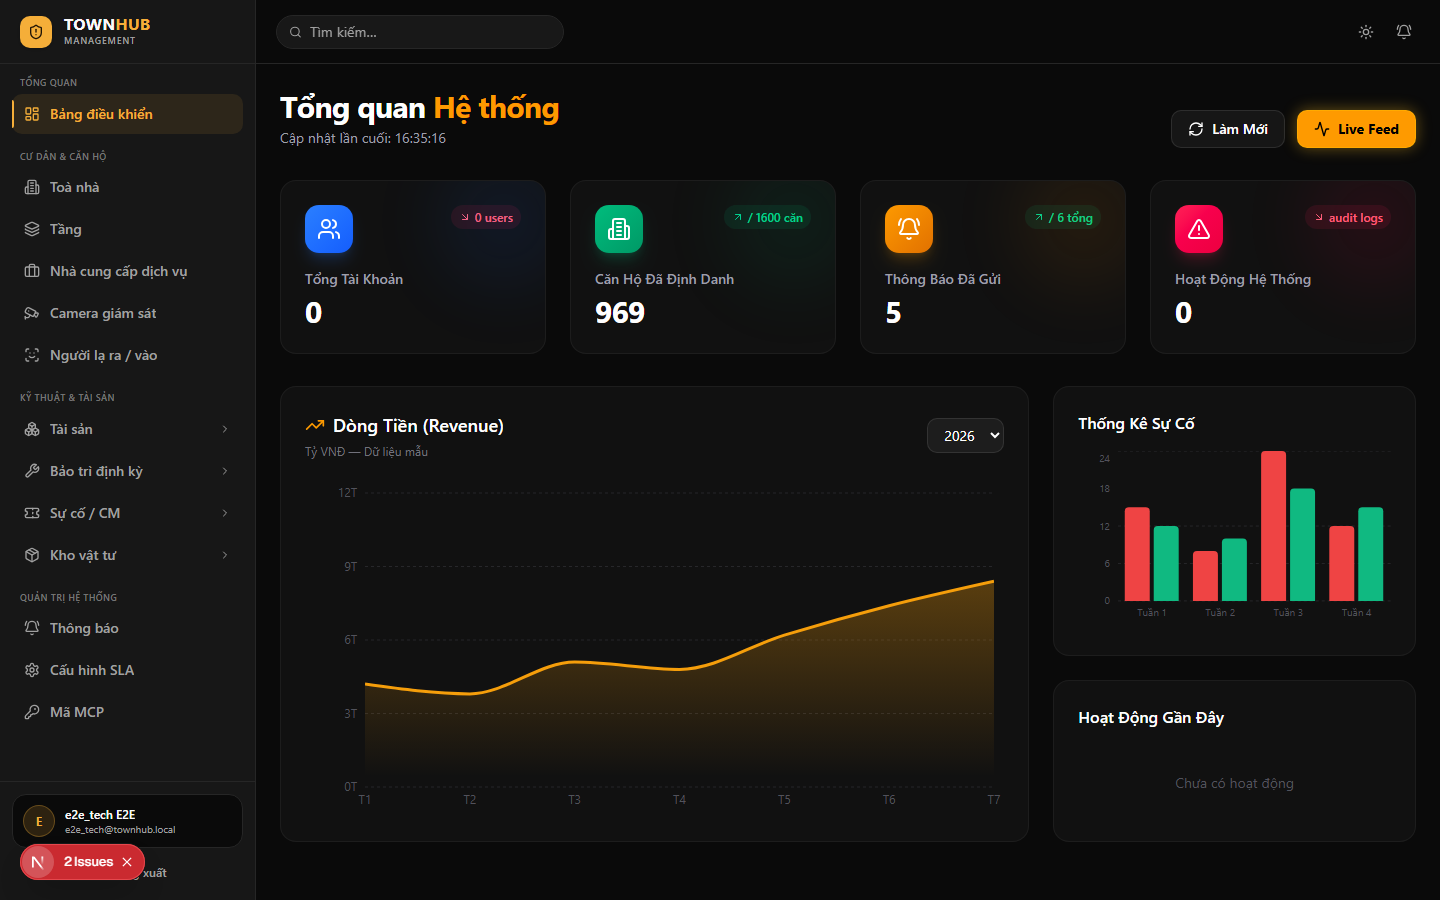
\includegraphics[width=\linewidth,height=0.44\textheight,keepaspectratio]{images/tc_role_technician_dashboard.png}
\caption*{\small Hình PL.3. Giao diện đăng nhập vai trò \textbf{Kỹ thuật viên}.}
\end{figure}
\clearpage
\begin{figure}[H]\centering
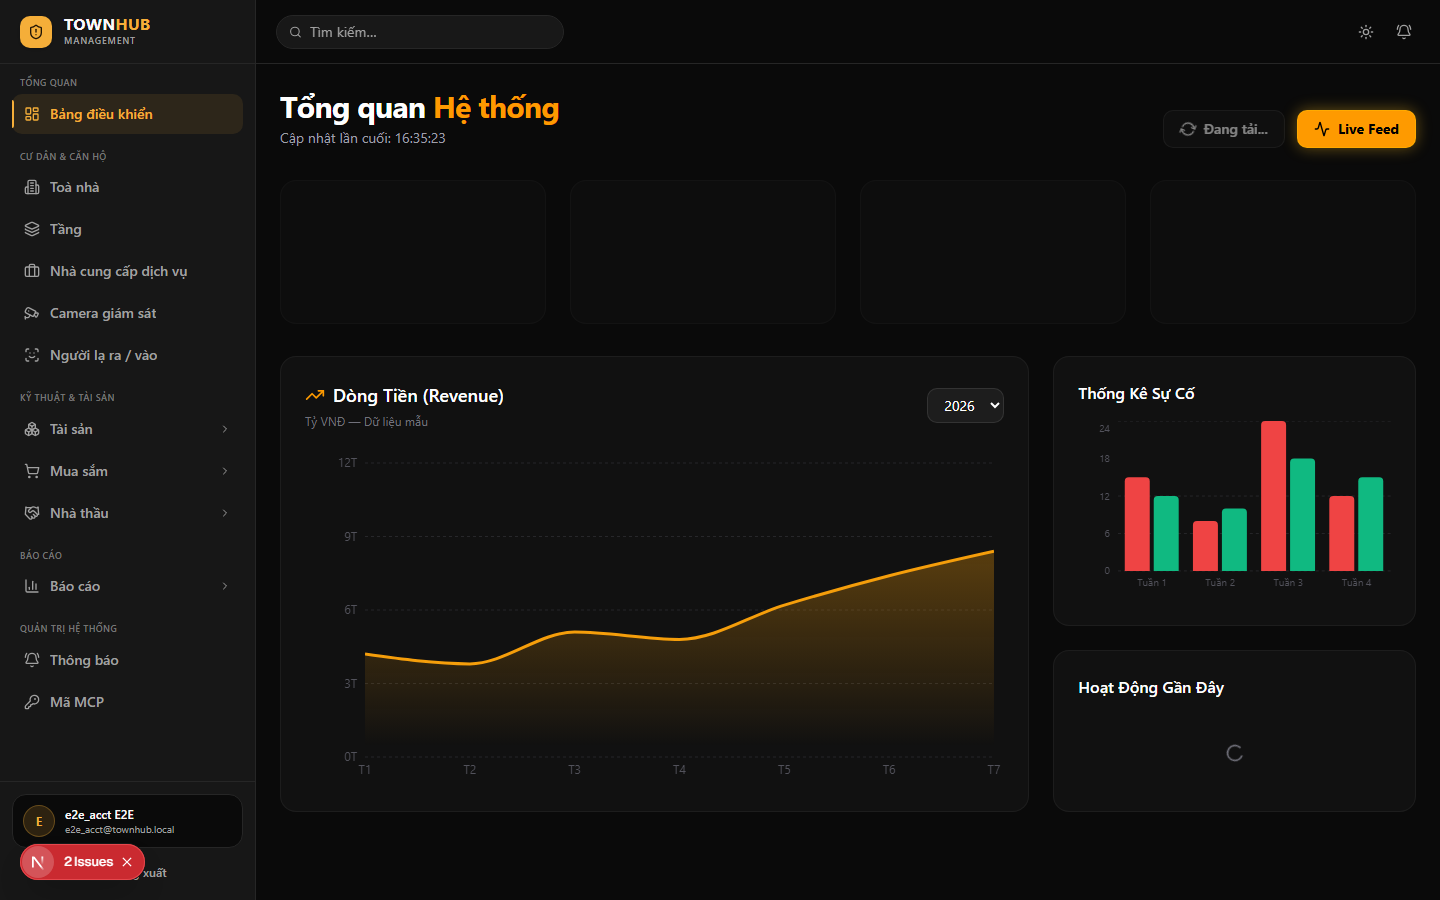
\includegraphics[width=\linewidth,height=0.44\textheight,keepaspectratio]{images/tc_role_accountant_dashboard.png}
\caption*{\small Hình PL.4. Giao diện đăng nhập vai trò \textbf{Kế toán}.}
\end{figure}
\begin{figure}[H]\centering
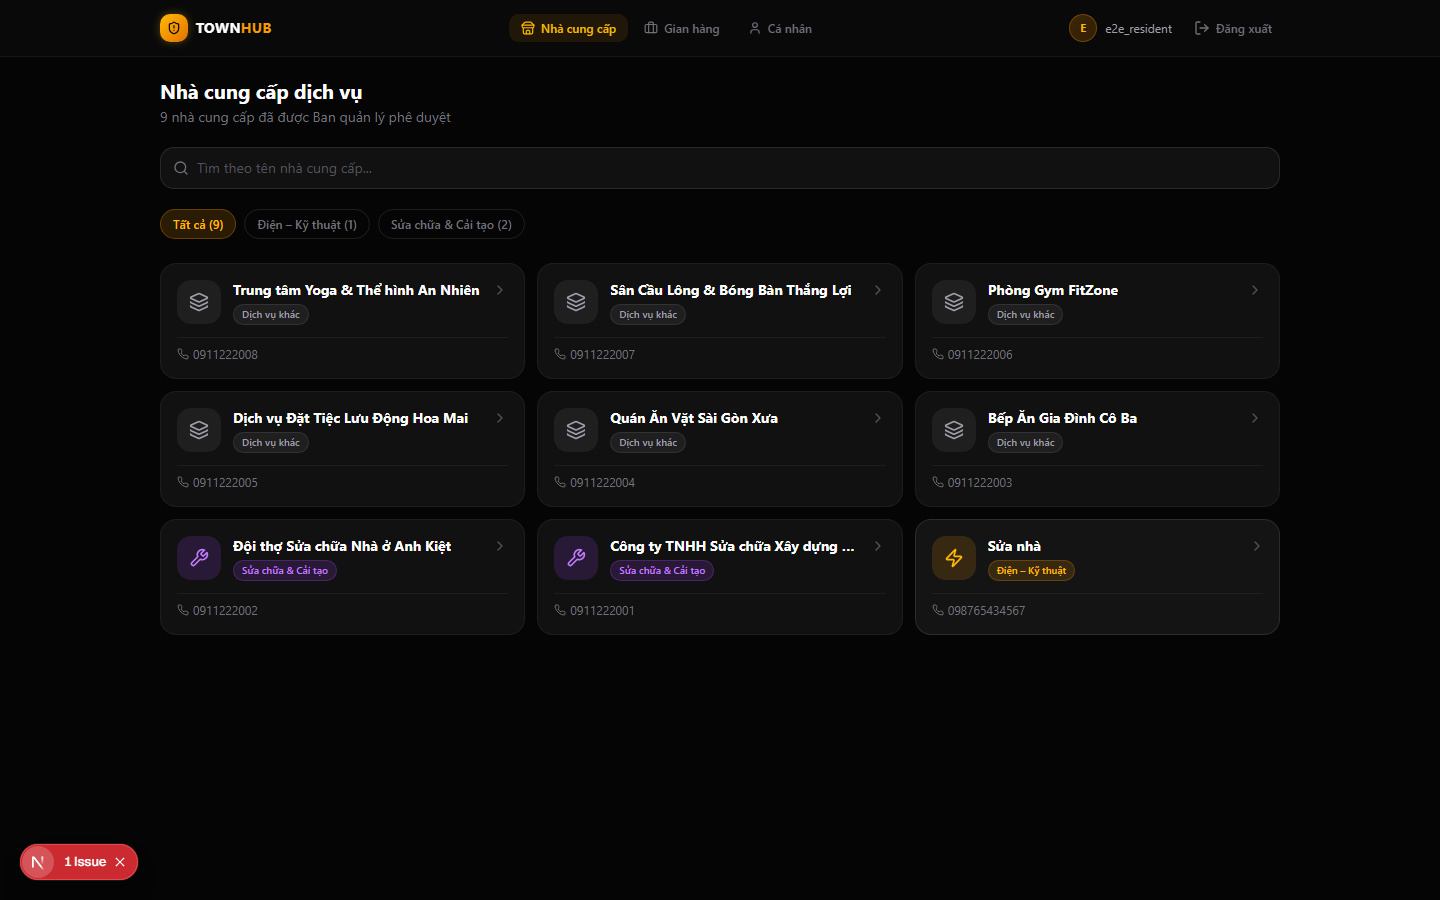
\includegraphics[width=\linewidth,height=0.44\textheight,keepaspectratio]{images/tc_role_resident_dashboard.png}
\caption*{\small Hình PL.5. Giao diện đăng nhập vai trò \textbf{Cư dân}.}
\end{figure}
\begin{figure}[H]\centering
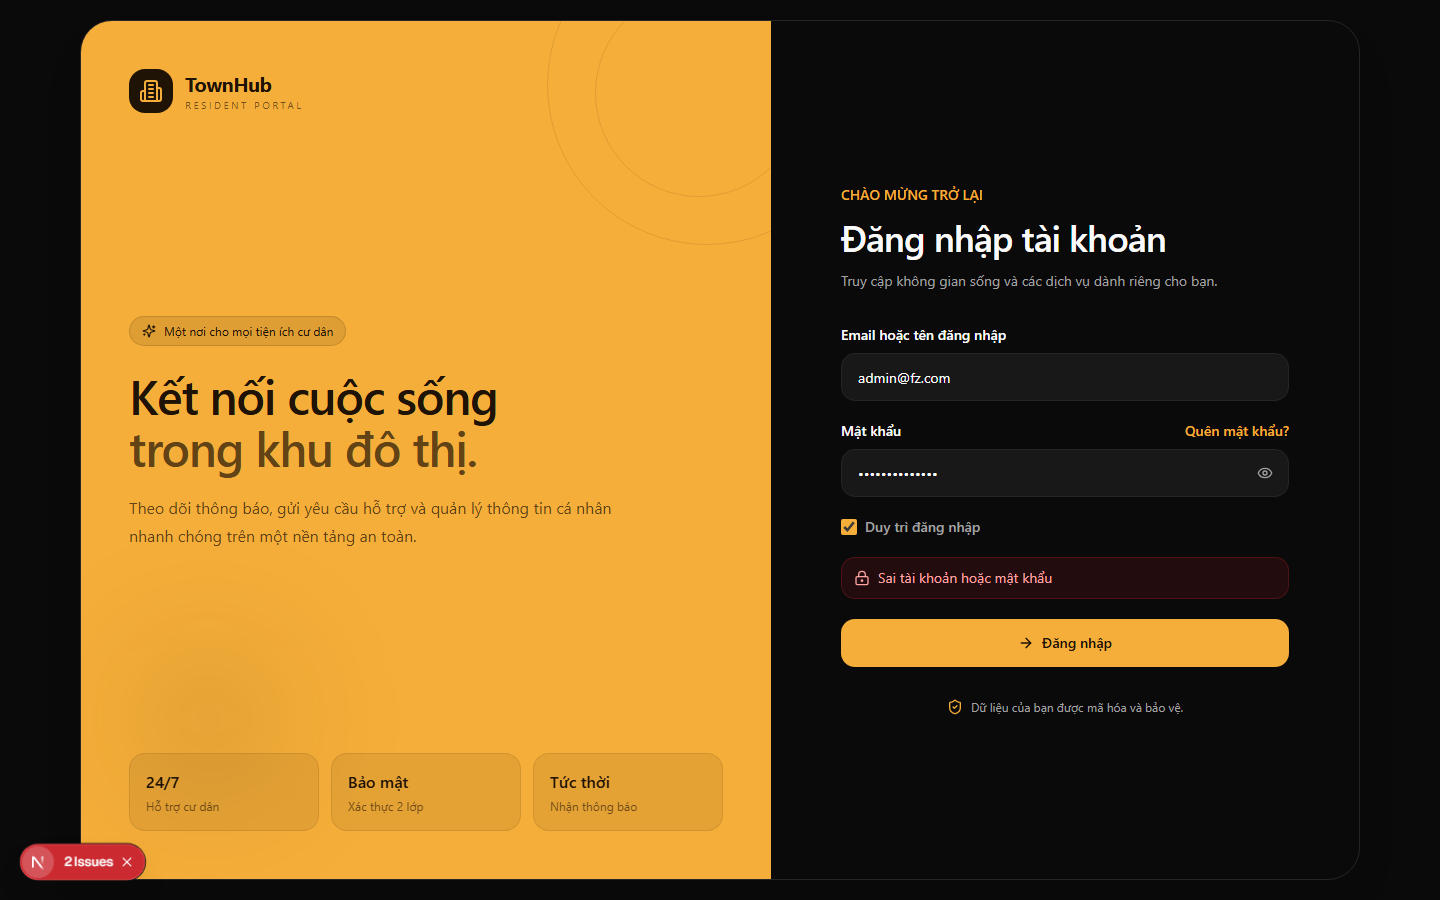
\includegraphics[width=\linewidth,height=0.44\textheight,keepaspectratio]{images/tc_auth_03_wrong_password.png}
\caption*{\small Hình PL.6. Ca side: đăng nhập sai mật khẩu bị báo lỗi.}
\end{figure}

\clearpage
\textbf{Ảnh minh hoạ 2 — Các màn hình nghiệp vụ được kiểm thử.}

\begin{figure}[H]\centering
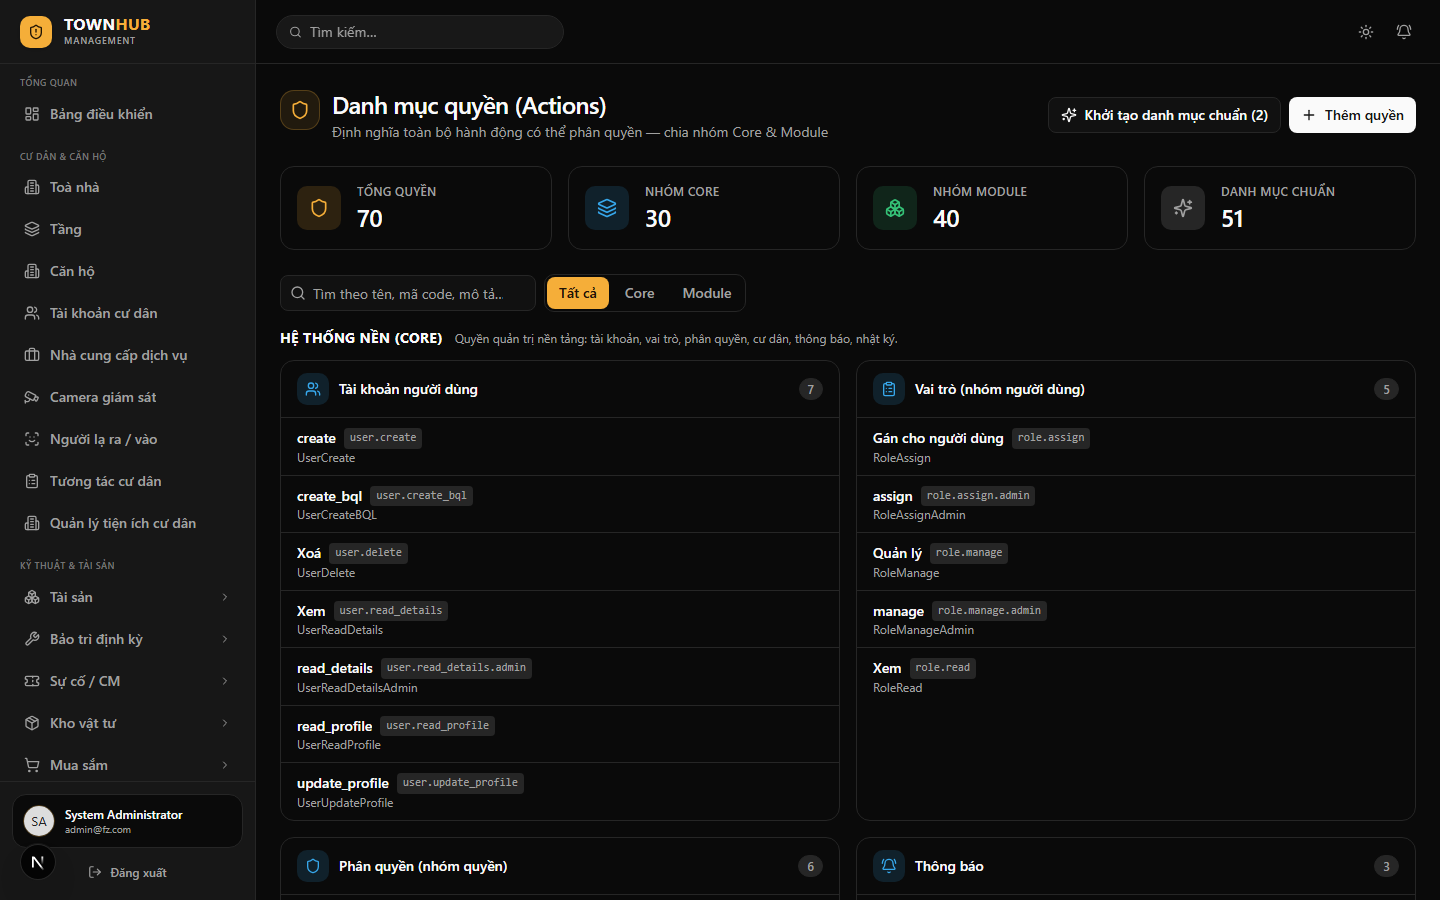
\includegraphics[width=\linewidth,height=0.44\textheight,keepaspectratio]{images/tc_auth_22_permissions.png}
\caption*{\small Hình PL.7. Danh mục quyền \& phân quyền (RBAC).}
\end{figure}
\begin{figure}[H]\centering
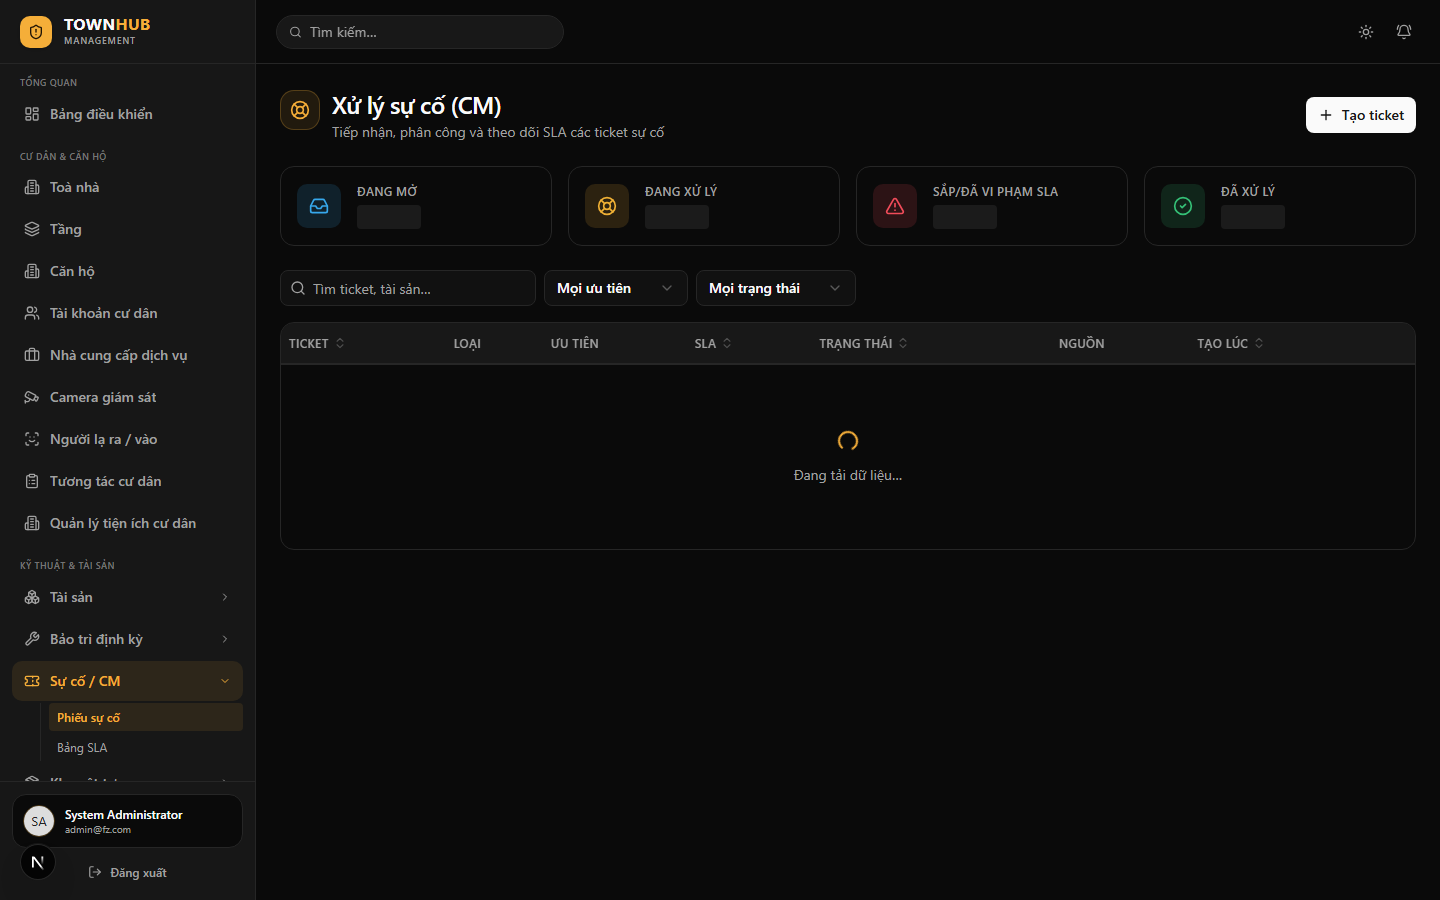
\includegraphics[width=\linewidth,height=0.44\textheight,keepaspectratio]{images/tc_ui_tickets.png}
\caption*{\small Hình PL.8. Danh sách ticket sự cố.}
\end{figure}
\begin{figure}[H]\centering
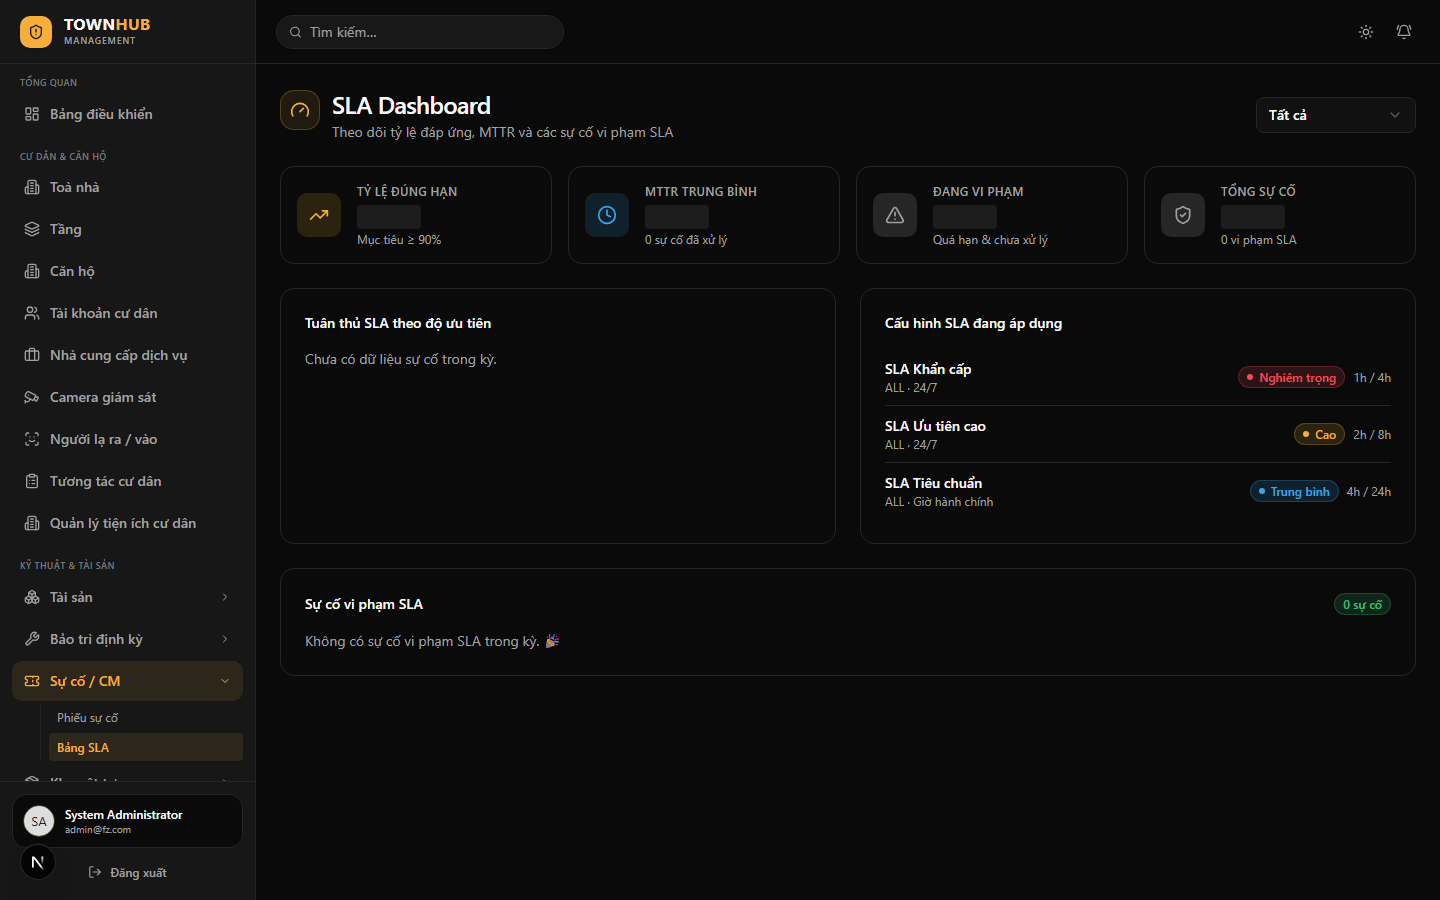
\includegraphics[width=\linewidth,height=0.44\textheight,keepaspectratio]{images/tc_ui_sla_dashboard.png}
\caption*{\small Hình PL.9. Bảng theo dõi SLA.}
\end{figure}
\clearpage
\begin{figure}[H]\centering
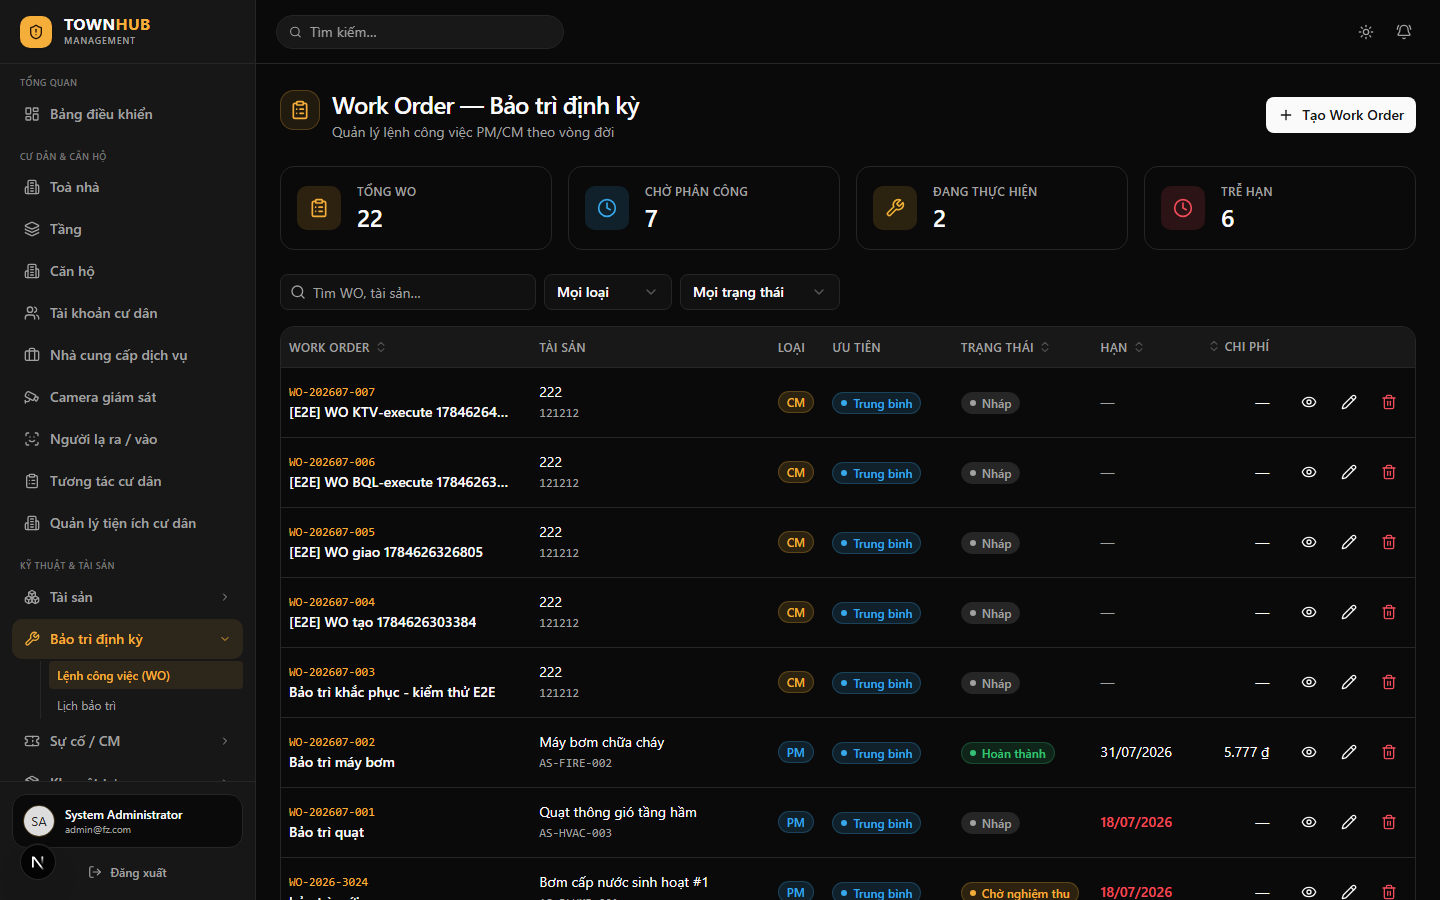
\includegraphics[width=\linewidth,height=0.44\textheight,keepaspectratio]{images/tc_ui_work_orders.png}
\caption*{\small Hình PL.10. Danh sách lệnh công việc (Work Order).}
\end{figure}
\begin{figure}[H]\centering
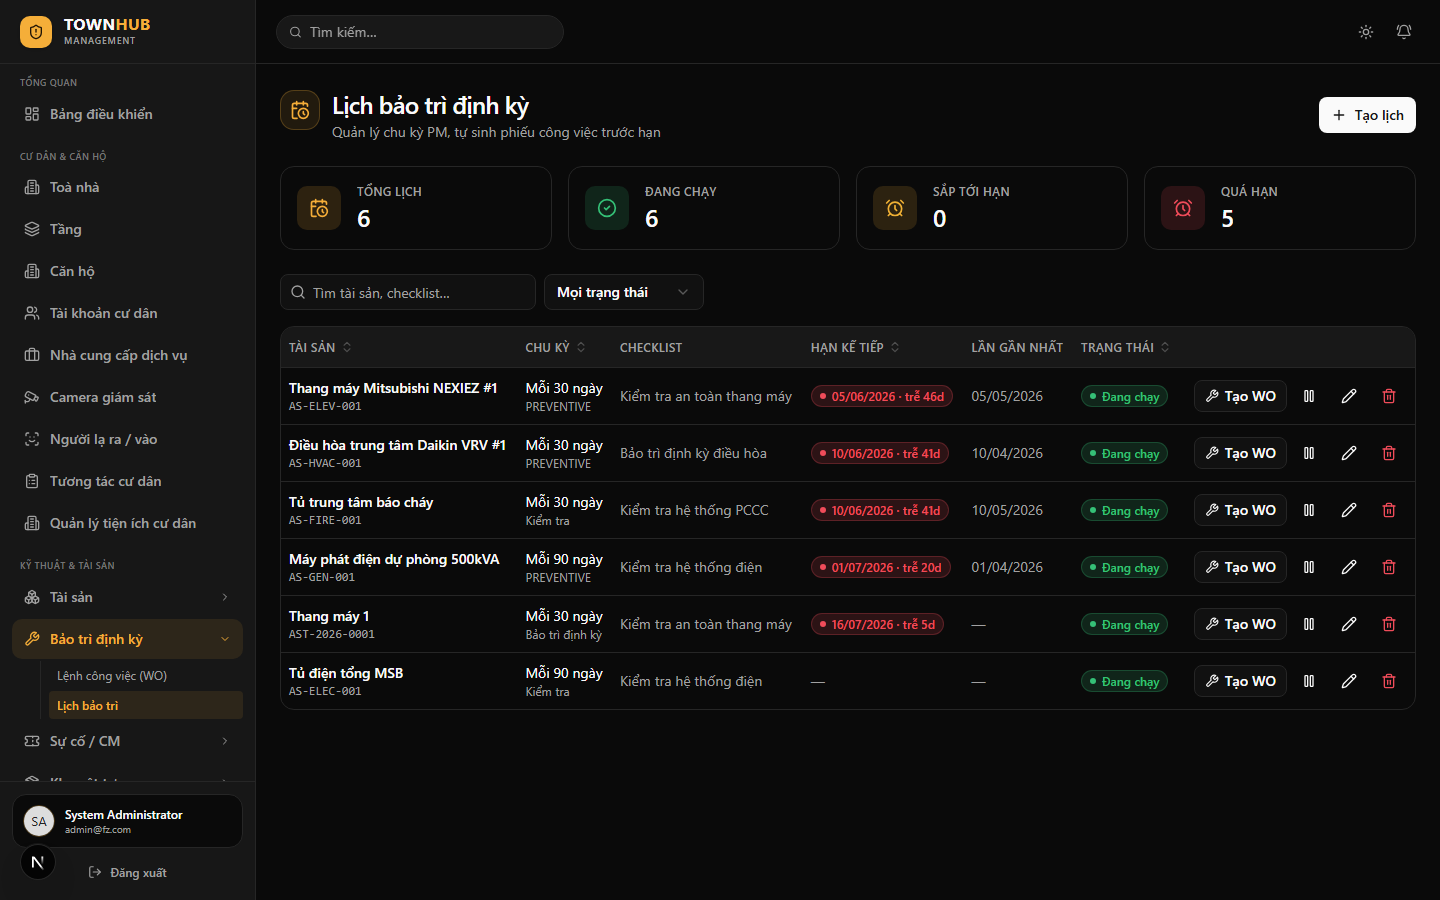
\includegraphics[width=\linewidth,height=0.44\textheight,keepaspectratio]{images/tc_ui_pm_schedules.png}
\caption*{\small Hình PL.11. Lịch bảo trì định kỳ.}
\end{figure}
\begin{figure}[H]\centering
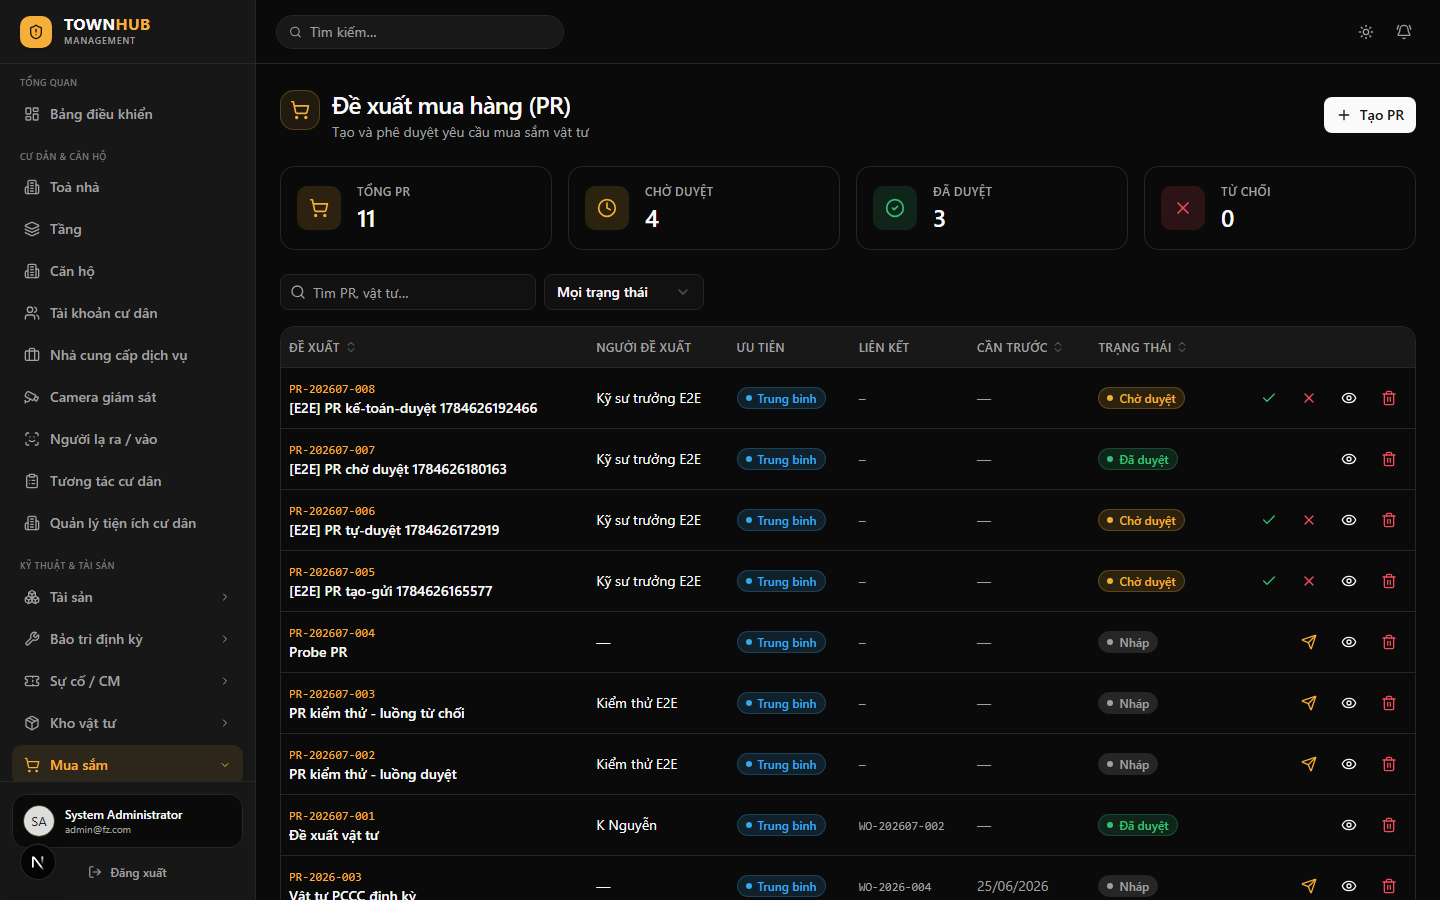
\includegraphics[width=\linewidth,height=0.44\textheight,keepaspectratio]{images/tc_ui_proc_requests.png}
\caption*{\small Hình PL.12. Phiếu yêu cầu mua sắm (PR).}
\end{figure}
\clearpage
\begin{figure}[H]\centering
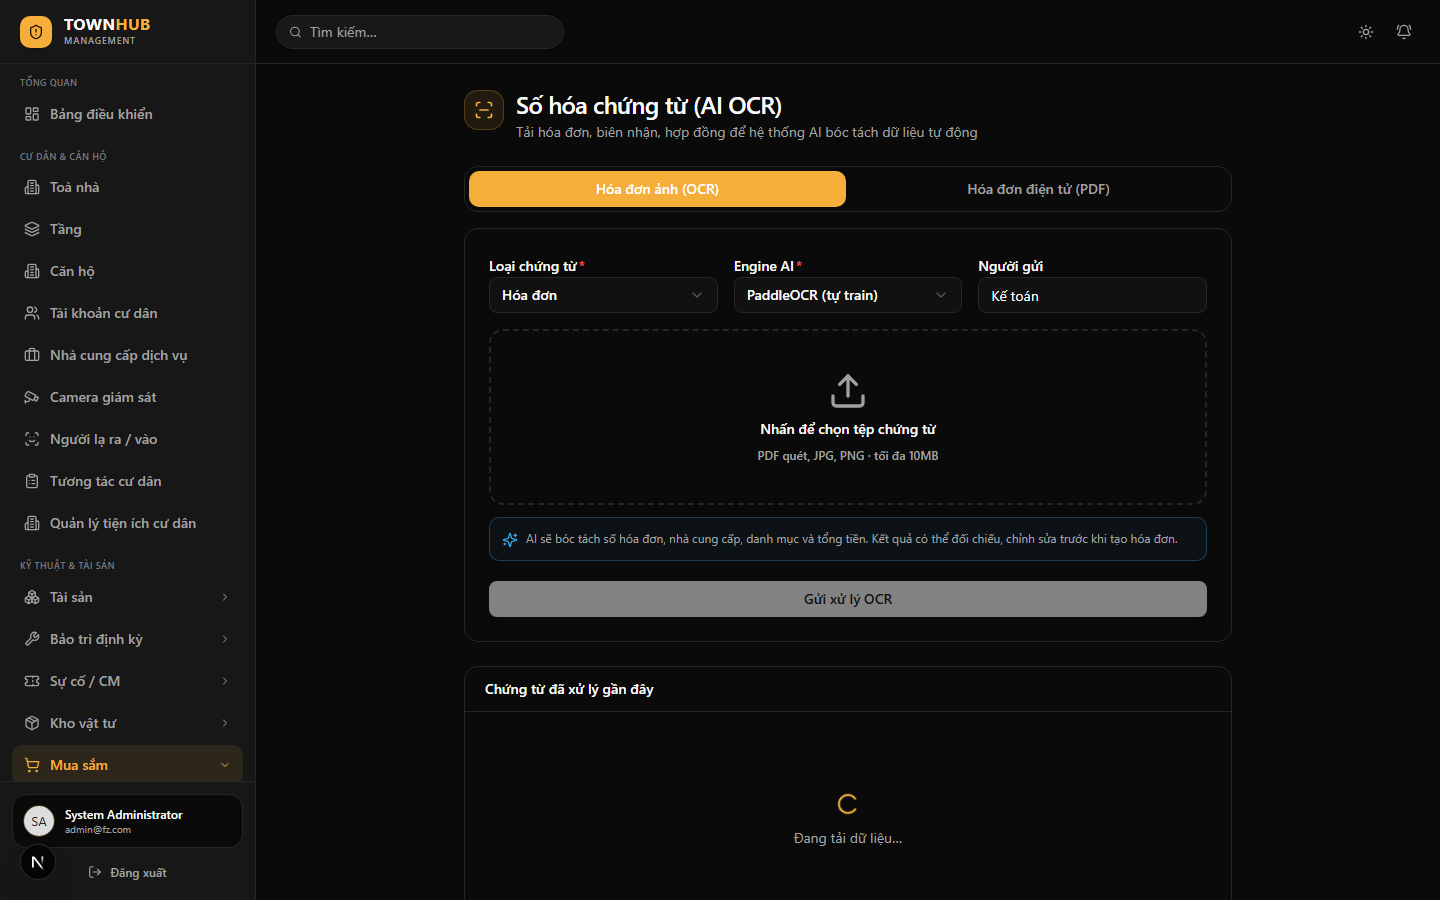
\includegraphics[width=\linewidth,height=0.44\textheight,keepaspectratio]{images/tc_ui_proc_ocr_new.png}
\caption*{\small Hình PL.13. Màn hình tải hoá đơn cho OCR.}
\end{figure}
\begin{figure}[H]\centering
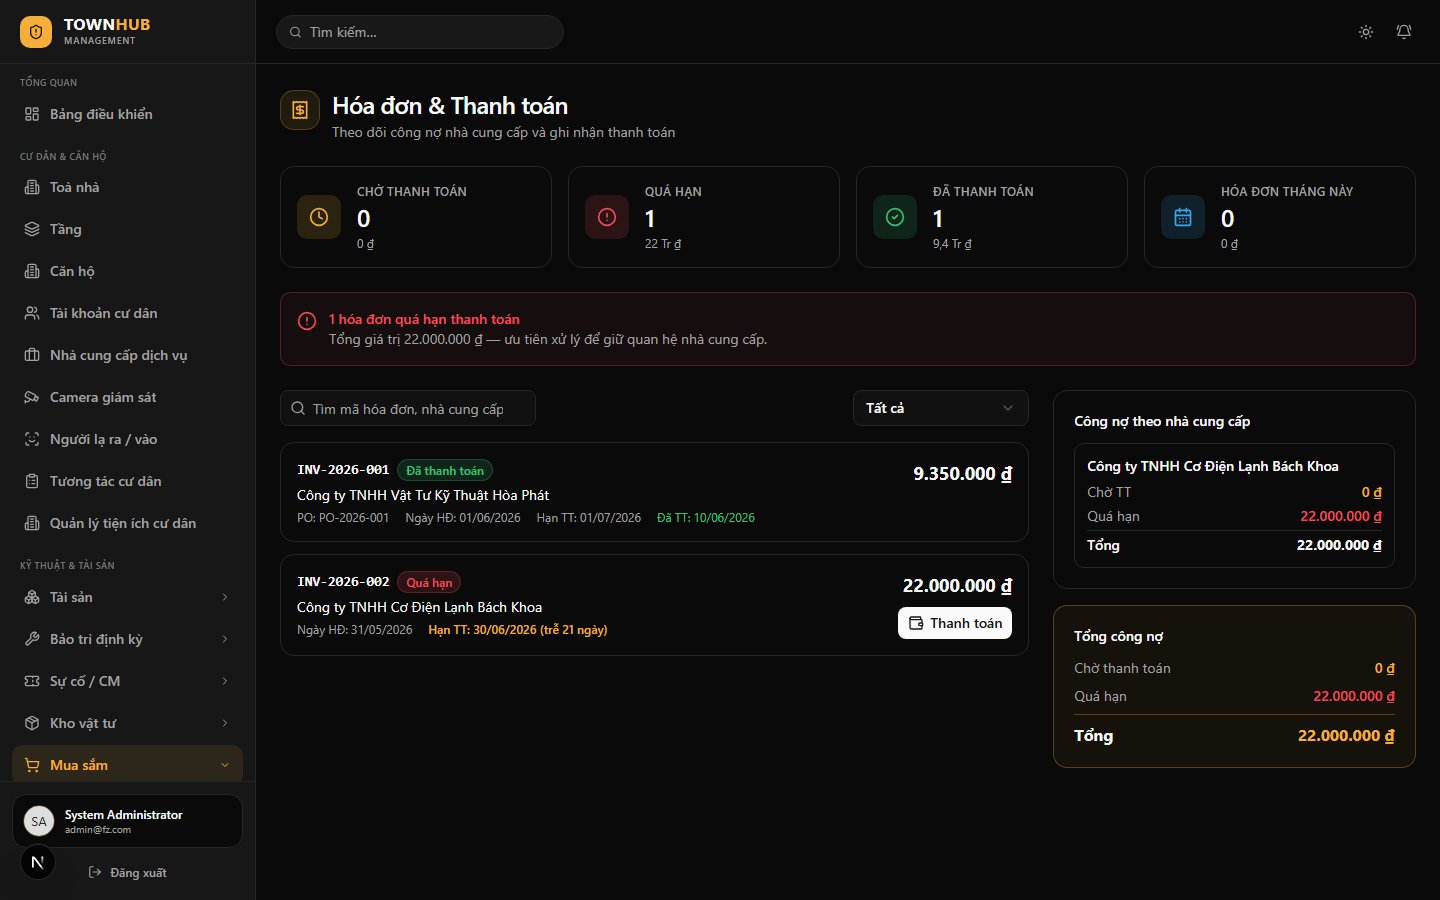
\includegraphics[width=\linewidth,height=0.44\textheight,keepaspectratio]{images/tc_ui_proc_invoices.png}
\caption*{\small Hình PL.14. Danh sách hoá đơn.}
\end{figure}
\begin{figure}[H]\centering
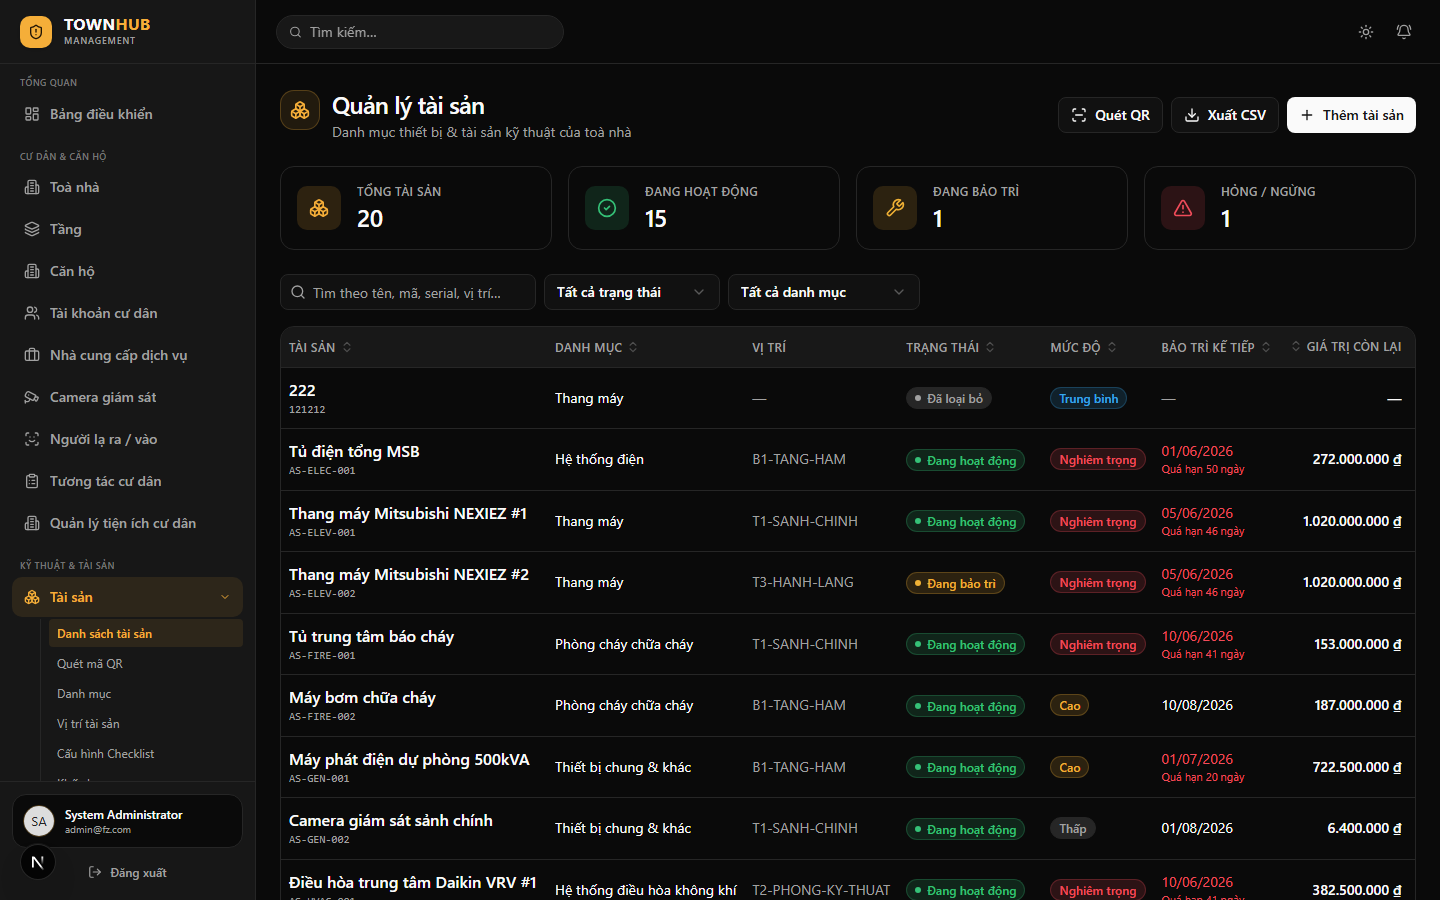
\includegraphics[width=\linewidth,height=0.44\textheight,keepaspectratio]{images/tc_ui_assets_list.png}
\caption*{\small Hình PL.15. Danh sách tài sản.}
\end{figure}
\clearpage
\begin{figure}[H]\centering
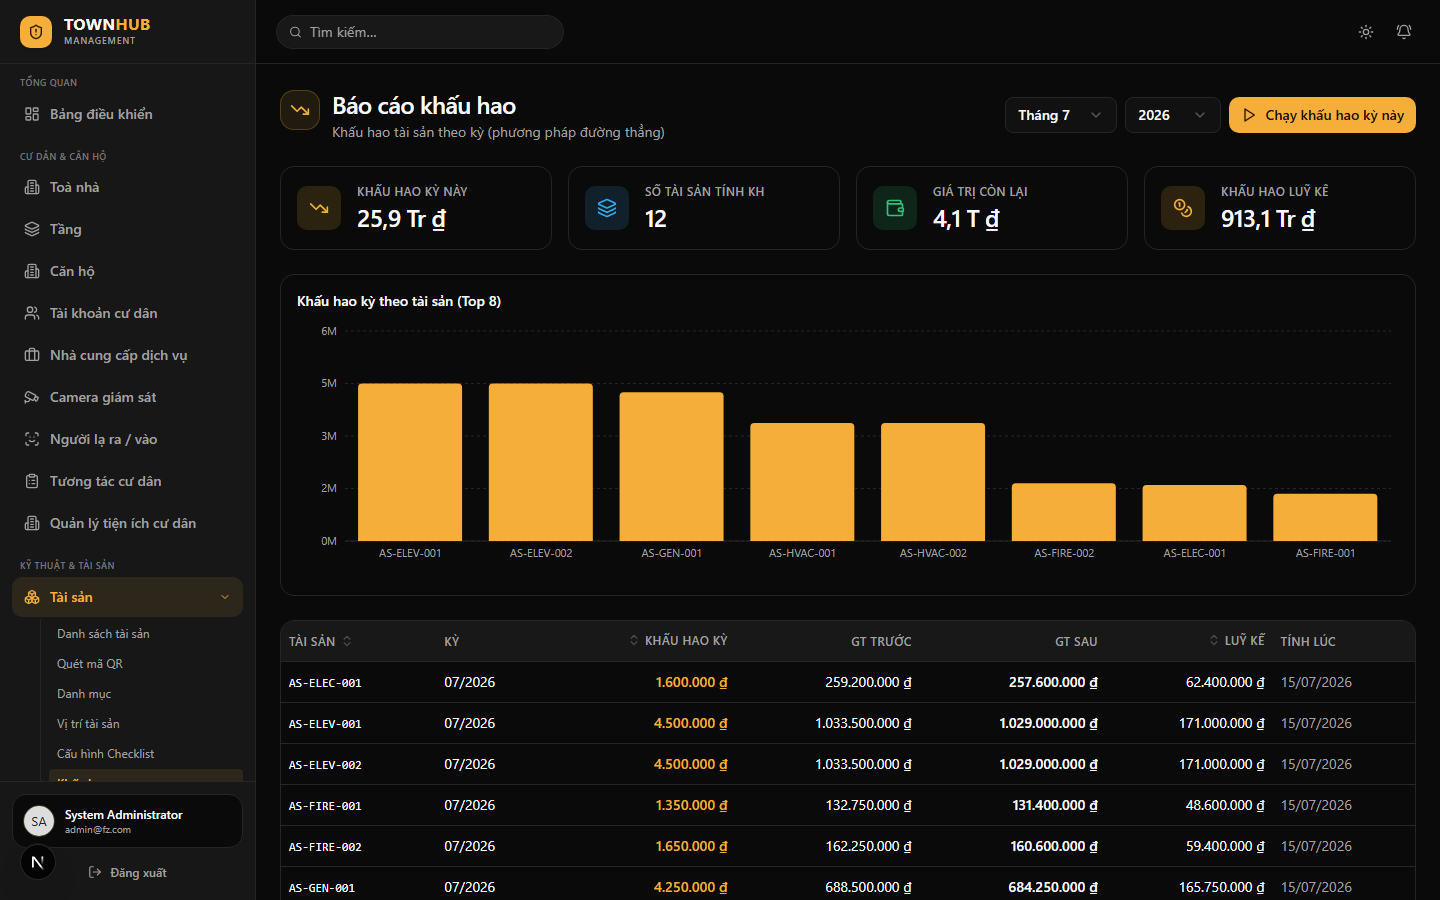
\includegraphics[width=\linewidth,height=0.44\textheight,keepaspectratio]{images/tc_ui_assets_depreciation.png}
\caption*{\small Hình PL.16. Khấu hao tài sản.}
\end{figure}
\begin{figure}[H]\centering
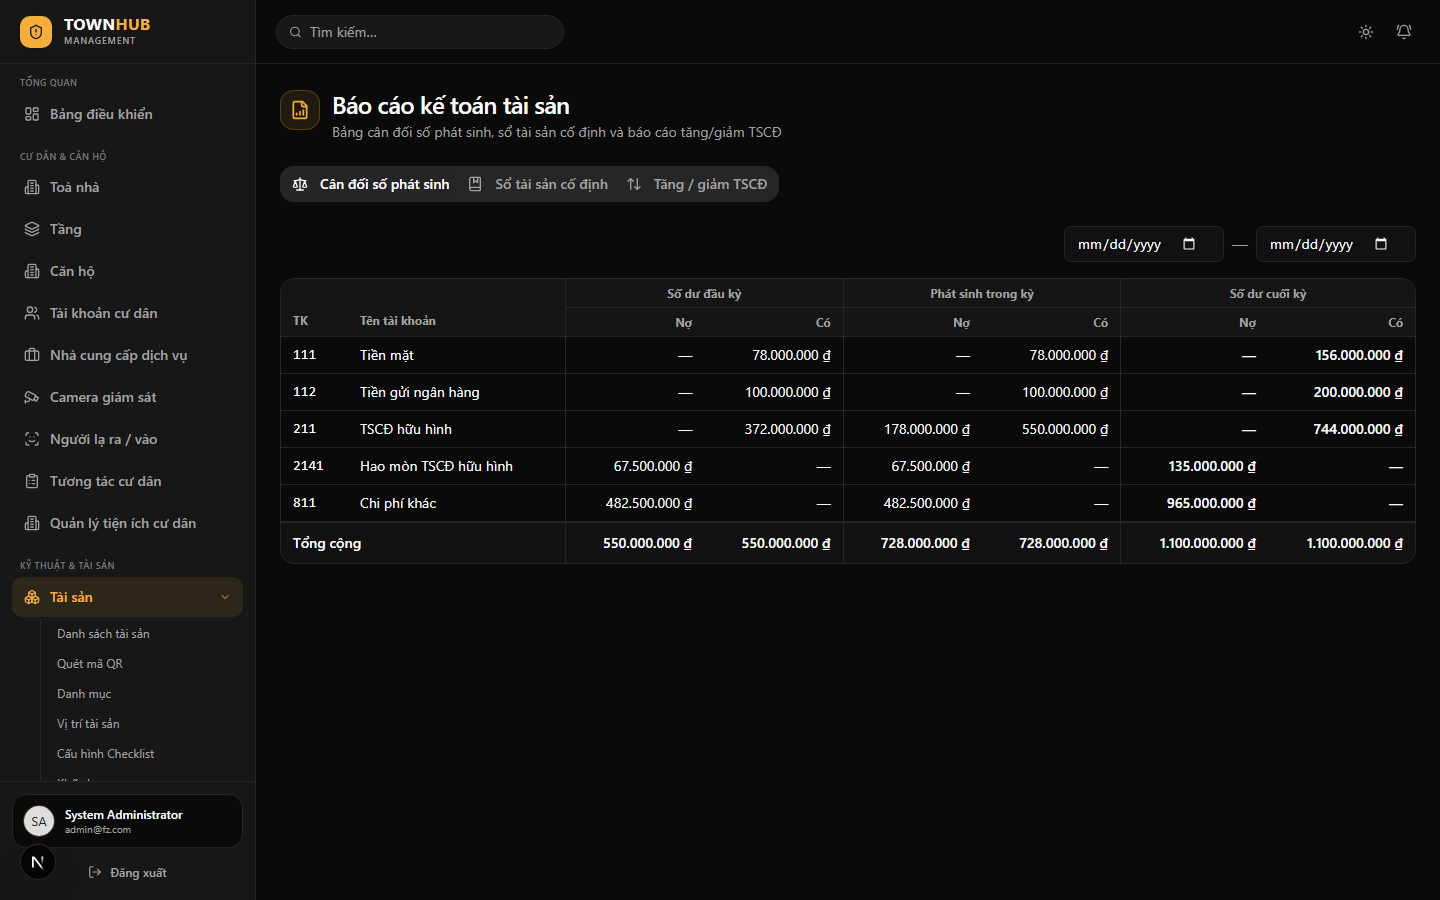
\includegraphics[width=\linewidth,height=0.44\textheight,keepaspectratio]{images/tc_ui_assets_reports.png}
\caption*{\small Hình PL.17. Báo cáo tài sản (kế toán).}
\end{figure}

